\PassOptionsToPackage{unicode=true}{hyperref} % options for packages loaded elsewhere
\PassOptionsToPackage{hyphens}{url}
%
\documentclass[]{book}
\usepackage{lmodern}
\usepackage{amssymb,amsmath}
\usepackage{ifxetex,ifluatex}
\usepackage{fixltx2e} % provides \textsubscript
\ifnum 0\ifxetex 1\fi\ifluatex 1\fi=0 % if pdftex
  \usepackage[T1]{fontenc}
  \usepackage[utf8]{inputenc}
  \usepackage{textcomp} % provides euro and other symbols
\else % if luatex or xelatex
  \usepackage{unicode-math}
  \defaultfontfeatures{Ligatures=TeX,Scale=MatchLowercase}
\fi
% use upquote if available, for straight quotes in verbatim environments
\IfFileExists{upquote.sty}{\usepackage{upquote}}{}
% use microtype if available
\IfFileExists{microtype.sty}{%
\usepackage[]{microtype}
\UseMicrotypeSet[protrusion]{basicmath} % disable protrusion for tt fonts
}{}
\IfFileExists{parskip.sty}{%
\usepackage{parskip}
}{% else
\setlength{\parindent}{0pt}
\setlength{\parskip}{6pt plus 2pt minus 1pt}
}
\usepackage{hyperref}
\hypersetup{
            pdftitle={Learning Statistical Models Through Simulation in R},
            pdfauthor={Dale J. Barr},
            pdfborder={0 0 0},
            breaklinks=true}
\urlstyle{same}  % don't use monospace font for urls
\usepackage{color}
\usepackage{fancyvrb}
\newcommand{\VerbBar}{|}
\newcommand{\VERB}{\Verb[commandchars=\\\{\}]}
\DefineVerbatimEnvironment{Highlighting}{Verbatim}{commandchars=\\\{\}}
% Add ',fontsize=\small' for more characters per line
\usepackage{framed}
\definecolor{shadecolor}{RGB}{248,248,248}
\newenvironment{Shaded}{\begin{snugshade}}{\end{snugshade}}
\newcommand{\AlertTok}[1]{\textcolor[rgb]{0.94,0.16,0.16}{#1}}
\newcommand{\AnnotationTok}[1]{\textcolor[rgb]{0.56,0.35,0.01}{\textbf{\textit{#1}}}}
\newcommand{\AttributeTok}[1]{\textcolor[rgb]{0.77,0.63,0.00}{#1}}
\newcommand{\BaseNTok}[1]{\textcolor[rgb]{0.00,0.00,0.81}{#1}}
\newcommand{\BuiltInTok}[1]{#1}
\newcommand{\CharTok}[1]{\textcolor[rgb]{0.31,0.60,0.02}{#1}}
\newcommand{\CommentTok}[1]{\textcolor[rgb]{0.56,0.35,0.01}{\textit{#1}}}
\newcommand{\CommentVarTok}[1]{\textcolor[rgb]{0.56,0.35,0.01}{\textbf{\textit{#1}}}}
\newcommand{\ConstantTok}[1]{\textcolor[rgb]{0.00,0.00,0.00}{#1}}
\newcommand{\ControlFlowTok}[1]{\textcolor[rgb]{0.13,0.29,0.53}{\textbf{#1}}}
\newcommand{\DataTypeTok}[1]{\textcolor[rgb]{0.13,0.29,0.53}{#1}}
\newcommand{\DecValTok}[1]{\textcolor[rgb]{0.00,0.00,0.81}{#1}}
\newcommand{\DocumentationTok}[1]{\textcolor[rgb]{0.56,0.35,0.01}{\textbf{\textit{#1}}}}
\newcommand{\ErrorTok}[1]{\textcolor[rgb]{0.64,0.00,0.00}{\textbf{#1}}}
\newcommand{\ExtensionTok}[1]{#1}
\newcommand{\FloatTok}[1]{\textcolor[rgb]{0.00,0.00,0.81}{#1}}
\newcommand{\FunctionTok}[1]{\textcolor[rgb]{0.00,0.00,0.00}{#1}}
\newcommand{\ImportTok}[1]{#1}
\newcommand{\InformationTok}[1]{\textcolor[rgb]{0.56,0.35,0.01}{\textbf{\textit{#1}}}}
\newcommand{\KeywordTok}[1]{\textcolor[rgb]{0.13,0.29,0.53}{\textbf{#1}}}
\newcommand{\NormalTok}[1]{#1}
\newcommand{\OperatorTok}[1]{\textcolor[rgb]{0.81,0.36,0.00}{\textbf{#1}}}
\newcommand{\OtherTok}[1]{\textcolor[rgb]{0.56,0.35,0.01}{#1}}
\newcommand{\PreprocessorTok}[1]{\textcolor[rgb]{0.56,0.35,0.01}{\textit{#1}}}
\newcommand{\RegionMarkerTok}[1]{#1}
\newcommand{\SpecialCharTok}[1]{\textcolor[rgb]{0.00,0.00,0.00}{#1}}
\newcommand{\SpecialStringTok}[1]{\textcolor[rgb]{0.31,0.60,0.02}{#1}}
\newcommand{\StringTok}[1]{\textcolor[rgb]{0.31,0.60,0.02}{#1}}
\newcommand{\VariableTok}[1]{\textcolor[rgb]{0.00,0.00,0.00}{#1}}
\newcommand{\VerbatimStringTok}[1]{\textcolor[rgb]{0.31,0.60,0.02}{#1}}
\newcommand{\WarningTok}[1]{\textcolor[rgb]{0.56,0.35,0.01}{\textbf{\textit{#1}}}}
\usepackage{longtable,booktabs}
% Fix footnotes in tables (requires footnote package)
\IfFileExists{footnote.sty}{\usepackage{footnote}\makesavenoteenv{longtable}}{}
\usepackage{graphicx,grffile}
\makeatletter
\def\maxwidth{\ifdim\Gin@nat@width>\linewidth\linewidth\else\Gin@nat@width\fi}
\def\maxheight{\ifdim\Gin@nat@height>\textheight\textheight\else\Gin@nat@height\fi}
\makeatother
% Scale images if necessary, so that they will not overflow the page
% margins by default, and it is still possible to overwrite the defaults
% using explicit options in \includegraphics[width, height, ...]{}
\setkeys{Gin}{width=\maxwidth,height=\maxheight,keepaspectratio}
\setlength{\emergencystretch}{3em}  % prevent overfull lines
\providecommand{\tightlist}{%
  \setlength{\itemsep}{0pt}\setlength{\parskip}{0pt}}
\setcounter{secnumdepth}{5}
% Redefines (sub)paragraphs to behave more like sections
\ifx\paragraph\undefined\else
\let\oldparagraph\paragraph
\renewcommand{\paragraph}[1]{\oldparagraph{#1}\mbox{}}
\fi
\ifx\subparagraph\undefined\else
\let\oldsubparagraph\subparagraph
\renewcommand{\subparagraph}[1]{\oldsubparagraph{#1}\mbox{}}
\fi

% set default figure placement to htbp
\makeatletter
\def\fps@figure{htbp}
\makeatother

\usepackage{booktabs}
\usepackage{multicol}
\usepackage[framemethod=TikZ]{mdframed}
\usepackage{xcolor}

\newmdenv[%
        backgroundcolor=red!8,
        linecolor=red,
        outerlinewidth=1pt,
        roundcorner=5mm,
        skipabove=\baselineskip,
        skipbelow=\baselineskip
]{watchout}

\newmdenv[%
        backgroundcolor=yellow!8,
        linecolor=yellow,
        outerlinewidth=1pt,
        roundcorner=5mm,
        skipabove=\baselineskip,
        skipbelow=\baselineskip
]{warning}

\newmdenv[%
        backgroundcolor=blue!8,
        linecolor=blue,
        outerlinewidth=1pt,
        roundcorner=5mm,
        skipabove=\baselineskip,
        skipbelow=\baselineskip
]{info}

\newmdenv[%
        backgroundcolor=green!8,
        linecolor=green,
        outerlinewidth=1pt,
        roundcorner=5mm,
        skipabove=\baselineskip,
        skipbelow=\baselineskip
]{try}
\usepackage{booktabs}
\usepackage{longtable}
\usepackage{array}
\usepackage{multirow}
\usepackage{wrapfig}
\usepackage{float}
\usepackage{colortbl}
\usepackage{pdflscape}
\usepackage{tabu}
\usepackage{threeparttable}
\usepackage{threeparttablex}
\usepackage[normalem]{ulem}
\usepackage{makecell}
\usepackage{xcolor}
\usepackage[]{natbib}
\bibliographystyle{apalike}

\title{Learning Statistical Models Through Simulation in R}
\author{Dale J. Barr}
\date{2020-12-31}

\begin{document}
\maketitle

{
\setcounter{tocdepth}{1}
\tableofcontents
}
\hypertarget{overview}{%
\chapter*{Overview}\label{overview}}
\addcontentsline{toc}{chapter}{Overview}

This textbook approaches statistical analysis through the General Linear Model, taking a simulation-based approach in the R software environment. The overarching goal is to teach students how to translate a description of the design of a study into a linear model to analyze data from that study. The focus is on the skills needed to analyze data from psychology experiments.

The following topics are covered:

\begin{itemize}
\tightlist
\item
  linear modeling workflow;
\item
  variance-covariance matrices;
\item
  multiple regression;
\item
  interactions (continuous-by-categorical; categorical-by-categorical);
\item
  linear mixed-effects regression;
\item
  generalized linear mixed-effects regression.
\end{itemize}

The material in this course forms the basis for a one-semester course for third-year undergradautes taught by \href{}{Dale Barr} at the \href{}{University of Glasgow School of Psychology}. It is part of the \href{https://psyteachr.github.io}{PsyTeachR series of course materials} developed by University of Glasgow Psychology staff.

Unlike other textbooks you may have encountered, this is an \textbf{interactive textbook}. Each chapter contains embedded exercises as well as web applications to help students better understand the content. The interactive content will only work if you access this material through a web browser. Printing out the material is not recommended. If you want to access the textbook without an internet connection or have a local version to keep in case this site changes or moves, you can \href{offline-textbook.zip}{download a version for offline use}. Just extract the files from the ZIP archive, locate the file \texttt{index.html} in the \texttt{docs} directory, and open this file using a web browser.

\hypertarget{how-to-cite-this-book}{%
\section*{How to cite this book}\label{how-to-cite-this-book}}
\addcontentsline{toc}{section}{How to cite this book}

Barr, Dale J. (2020). \emph{Learning statistical models through simulation in R: An interactive textbook}. Version 0.9-3. Retrieved from \url{https://psyteachr.github.io/book/ug3-stats}.

\hypertarget{information-for-educators}{%
\section*{Information for educators}\label{information-for-educators}}
\addcontentsline{toc}{section}{Information for educators}

You are free to re-use and modify the material in this textbook for your own purposes, with the stipulation that you cite the original work. Please note additional terms of the \href{https://creativecommons.org/licenses/by-sa/4.0/}{Creative Commons CC-BY-SA 4.0 license} governing re-use of this material.

The book was built using the R \href{https://bookdown.org}{\textbf{\texttt{bookdown}}} package. The source files are available at \href{https://github.com/psyteachr/ug3-stats}{github}.

\hypertarget{introduction}{%
\chapter{Introduction}\label{introduction}}

\hypertarget{goal-of-this-course}{%
\section{Goal of this course}\label{goal-of-this-course}}

The goal of this course is to teach you how to simulate and analyze the various types of datasets you are likely to encounter as a psychologist. The focus is on behavioral data---e.g., measures of reaction time, perceptual judgments, choices, decision, ratings on a survey, hours of sleep, etc.---usually collected in the context of a study or experiment.

In its approach to statistical analysis, this course attempts to maximize \textbf{flexibility}, \textbf{generalizability}, and \textbf{reproducibility}. You may have heard talk in the media about psychology being in the throes of various `crises'. There have been some high-profile replication failures that have contributed to the impression that all is not well. There have also been a number of demonstrations that the standard approaches to data analysis in psychology are flawed, in that they allow researchers to present results as clean-cut and confirmatory while hiding various analyses that have been pursued and discarded while seeking to attain the desired result. But it is not just the field of psychology where such problems can be found---the problem is widespread, encompassing other fields of study as well. And the truth is that a certain level of self-criticism and self-reflection can also be seen positively---as a sign of a healthy discipline. Whatever your take, there is room for improvement, and the purpose of this course is to give you tools to ensure that your own analyses are not only statistically sound, but also as generalizable and reproducible as possible.

\hypertarget{flexibility}{%
\subsection{Flexibility}\label{flexibility}}

The approach taken in this course differs from other courses in that it emphasizes learning a flexible regression modeling framework rather than teaching `recipes' for dealing with different types of data, and assumes that the fundamental type of data you will need to analyze will be multilevel and also that you will need to deal not only with continuous measurements but also ordinal measurements (ratings on a Likert scale), counts (number of times particular event types have taken place), and nominal data (what category something falls into).

The most flexible approach available is the General Linear Model approach, in which some response variable is modeled in terms of a weighted linear sum of predictor variables. A simple mathematical example of one such formula is

\[Y_i = \beta_0 + \beta_1 X_i + e_i\]

where \(Y_i\) is the measured response for observation \(i\), modeled in terms of an intercept term plus the effect of predictor \(X_i\) weighted by coefficient \(\beta_1\) and residual error term \(e_i\), which reflects unmodeled variance.

You might recognize the above equation as representing the equation for a line (\(y = mx + b\)), with \(\beta_0\) playing the role of the y-intercept and \(\beta_1\) playing the role of the slope. The \(e_i\) term reflects what is left of observation \(i\) after accounting for the the intercept and the predictor \(X_i\).

A terminological convention in this course is that Greek letters (\(\beta\), \(\rho\), \(\tau\)) represent unobserved population parameters while Latin letters (\(X\), \(Y\)) represent observed values.

This linear formulation is highly general, and we will see how it can be used to model different kinds of relationships between different kinds of variables. One limitation of the current course is that it focuses mainly on univariate data, where a single response variable is the focus of analysis. It is often the case that you will be dealing with multiple response variables on the same subjects, but modeling them all simultaneously is technically very difficult and beyond the scope of this course. A simpler approach (and the one adopted here) is to analyze each response variable in a separate univariate analysis.

\hypertarget{generalizability}{%
\section{Generalizability}\label{generalizability}}

The term generalizability refers to the degree to which findings from a study can be readily applied to situations beyond the particular context (subjects, stimuli, task, etc.) in which the data were collected. At best, our findings would apply to all members of the human species across a wide variety of contexts; at worst, they would apply only to those specific people observed in the specific context of our study. Most studies fall somewhere between these two opposing poles.

The generalizability of a finding depends on several factors: how the study was designed, what materials were used, how subjects were recruited, the nature of the task given to the subjects, \textbf{and the way the data were analyzed}. It is this last point that we will focus on in this course. When analyzing a dataset, if you want to make generalizable claims, you must make decisions about what would count as a replication of your study---about which aspects would remain fixed across replications, and which aspects you would allow to vary. Unfortunately, you will sometimes find that data have been analyzed in a way that does not support generalization in the broadest sense, often because analyses underestimate the influence of ideosyncratic features of stimulus materials or experimental task on the observed result \citep{yarkoni_2019}.

\hypertarget{reproduciblity-and-transparency}{%
\section{Reproduciblity and Transparency}\label{reproduciblity-and-transparency}}

The term reproducibility refers to the degree to which it is possible to reproduce the pattern of findings in a study under various circumstances.

We say a finding is \emph{analytically} or \emph{computationally} reproducible if, given the raw data, we can obtain the same pattern of results. Note that this is different from saying a finding is \textbf{replicable}, which refers to being able to reproduce the finding in \textbf{new samples.} There is not widespread agreement about these terms, but it is convenient to view analytic reproducibility and replicability as two different but related types of reproducibility, with the former capturing reproducibility across analysts (or among the same analysts over time) and the latter reflecting reproducibility across participants.

Ensuring that analyses are reproducible is a hard problem. If you fail to properly document your own analyses, or the software that you used gets modified or goes out of date and becomes unavailable, you may have trouble reproducing your own findings!

Another important property of analyses is transparency: the extent to which all the steps in some research study have been made available. A study may be transparent but not reproducible, and vice versa. It is important to use a workflow that promotes transparency. This makes the `edit-and-execute' workflow of script programming ideal for data analysis, far superior to the `point-and-click' workflow of most commercial statistical programs. By writing code, you make the logic and decision process explicit to others and easy to reconstruct.

\hypertarget{a-simulation-based-approach}{%
\section{A simulation-based approach}\label{a-simulation-based-approach}}

A final characteristic that distinguishes this course is that it uses a \textbf{simulation-based approach} to learning about statistical models. By data simulation we mean specifying a model to characterize a population of interest and then using the computer's random number generator to simulate the process of sampling data from that population. We will look at a simple example of this below.

The typical problem that you will face when you analyze data is that you won't know the `ground truth' about the population you are studying. You take a sample from that population, make some assumptions about how the observed data have been generated, and then use the observed data to estimate unknown population parameters and the uncertainty around these parameters.

Data simulation inverts this process. You to define the parameters of a model representing the ground truth about a (hypothetical) population and then generate data from it. You can then analyze the resulting data in the way that you normally would, and see how well your parameter estimates correspond to the true values.

Let's look at an example. Let's assume you are interested in the question of whether being a parent of a toddler `sharpens' your reflexes. If you've ever taken care of a toddler, you know that physical danger always seems imminent---they could fall of the chair they just climbed on, slam their finger in a door, bang their head on the corner of a table, etc.---so you need to be attentive and ready to act fast. You hypothesize that this vigilance will translate into faster response times in other situations where a toddler is not around, such as in a psychological laboratory. So you recruit a set of parents of toddlers to come into the lab. You give each parent the task of pressing a button as quickly as possible in response to a flashing light, and measure their response time (in milliseconds). For each parent, you calculate their mean response time over all trials. We can simulate the mean response time for each of say, 50 parents using the \texttt{rnorm()} function in R. But before we do that, we will load in the packages that we need (tidyverse) and set the random seed to make sure that you (the reader) get the same random values as me (the author).

\begin{Shaded}
\begin{Highlighting}[]
\KeywordTok{library}\NormalTok{(}\StringTok{"tidyverse"}\NormalTok{)}

\KeywordTok{set.seed}\NormalTok{(}\DecValTok{2020}\NormalTok{)  }\CommentTok{# can be any arbitrary integer}
\end{Highlighting}
\end{Shaded}

\begin{Shaded}
\begin{Highlighting}[]
\NormalTok{parents <-}\StringTok{ }\KeywordTok{rnorm}\NormalTok{(}\DataTypeTok{n =} \DecValTok{50}\NormalTok{, }\DataTypeTok{mean =} \DecValTok{480}\NormalTok{, }\DataTypeTok{sd =} \DecValTok{40}\NormalTok{)}

\NormalTok{parents}
\end{Highlighting}
\end{Shaded}

\begin{verbatim}
##  [1] 495.0789 492.0619 436.0791 434.7838 368.1386 508.8229 517.5648 470.8249
##  [9] 550.3653 484.6947 445.8751 516.3704 527.8549 465.1366 475.0696 552.0017
## [17] 548.1598 358.4494 388.4410 482.3321 566.9746 523.9273 492.7288 477.0741
## [25] 513.3707 487.9500 531.9137 517.4687 474.1027 484.4173 447.4998 450.2519
## [33] 523.8138 577.4149 495.5247 491.6251 468.5761 483.0406 457.5881 497.8875
## [41] 516.3400 459.7976 467.9598 450.9586 432.7969 490.1230 465.1715 480.8872
## [49] 506.4018 499.5517
\end{verbatim}

We chose to generate the data using \texttt{rnorm()}---a function that generates random numbers from a normal distribution---reflecting our assumption that mean response time is normally distributed in the population. A normal distribution is defined by two parameters, a mean (usually notated with the Greek letter \(\mu\), pronounced ``myoo''), and a standard deviation (usually notated with the Greek letter \(\sigma\), pronounced ``sigma''). Since we have generated the data ourselves, both \(\mu\) and \(\sigma\) are known, and in the call to \texttt{rnorm()}, we set them to the values 480 and 40 respectively.

But of course, to test our hypothesis, we need a comparison group, so we define a control group of non-parents. We generate data from this control group in the same way as above, but changing the mean.

\begin{Shaded}
\begin{Highlighting}[]
\NormalTok{control <-}\StringTok{ }\KeywordTok{rnorm}\NormalTok{(}\DataTypeTok{n =} \DecValTok{50}\NormalTok{, }\DataTypeTok{mean =} \DecValTok{500}\NormalTok{, }\DataTypeTok{sd =} \DecValTok{40}\NormalTok{)}
\end{Highlighting}
\end{Shaded}

Let's put them into a tibble to make it easier to plot and analyze the data. Each row from this table represents the mean response time from a particular subject.

\begin{Shaded}
\begin{Highlighting}[]
\NormalTok{dat <-}\StringTok{ }\KeywordTok{tibble}\NormalTok{(}\DataTypeTok{group =} \KeywordTok{rep}\NormalTok{(}\KeywordTok{c}\NormalTok{(}\StringTok{"parent"}\NormalTok{, }\StringTok{"control"}\NormalTok{), }\KeywordTok{c}\NormalTok{(}\KeywordTok{length}\NormalTok{(parents), }\KeywordTok{length}\NormalTok{(control))),}
              \DataTypeTok{rt =} \KeywordTok{c}\NormalTok{(parents, control))}

\NormalTok{dat}
\end{Highlighting}
\end{Shaded}

\begin{verbatim}
## # A tibble: 100 x 2
##    group     rt
##    <chr>  <dbl>
##  1 parent  495.
##  2 parent  492.
##  3 parent  436.
##  4 parent  435.
##  5 parent  368.
##  6 parent  509.
##  7 parent  518.
##  8 parent  471.
##  9 parent  550.
## 10 parent  485.
## # ... with 90 more rows
\end{verbatim}

Here are some things to try with this simulated data.

\begin{enumerate}
\def\labelenumi{\arabic{enumi}.}
\tightlist
\item
  Plot the data in some sensible way.
\item
  Calculate means and standard deviations. How do they compare with the population parameters?
\item
  Run a t-test on these data. Is the effect of group significant?
\end{enumerate}

Once you have done these things, do them again, but changing the sample size, population parameters or both.

\hypertarget{what-you-will-learn}{%
\section{What you will learn}\label{what-you-will-learn}}

By the end of this course, you should be able to:

\begin{itemize}
\tightlist
\item
  simulate bivariate data
\item
  understand the relationship between correlation and regression
\item
  specify regression models to reflect various study designs
\item
  specify and interpret various types of interactions
\item
  simulate data from these models, including multilevel data
\item
  handle continuous, count, or nominal dependent variables.
\end{itemize}

\hypertarget{understanding-correlation-and-regression-through-bivariate-simulation}{%
\chapter{Understanding correlation and regression through bivariate simulation}\label{understanding-correlation-and-regression-through-bivariate-simulation}}

\begin{itemize}
\tightlist
\item
  Packages used:

  \begin{itemize}
  \tightlist
  \item
    \textbf{\texttt{tidyverse}}
  \item
    \textbf{\texttt{corrr}}
  \item
    \textbf{\texttt{MASS}} (built in)
  \end{itemize}
\item
  Functions used:

  \begin{itemize}
  \tightlist
  \item
    \texttt{base::choose()}
  \item
    \texttt{corrr::correlate()}
  \item
    \texttt{base::matrix()}
  \item
    \texttt{base::cor()}
  \item
    \texttt{base::log()} and \texttt{base::exp()} for log transformation (and back)
  \end{itemize}
\item
  Review

  \begin{itemize}
  \tightlist
  \item
    \href{https://psyteachr.github.io/ug2-practical/correlations.html}{L2 lab materials on correlation}.
  \end{itemize}
\end{itemize}

\hypertarget{correlation-matrices}{%
\section{Correlation matrices}\label{correlation-matrices}}

You may be familiar with the concept of a \textbf{correlation matrix} from reading papers in psychology. Correlation matrices are a common way of summarizing relationships between multiple measurements taken from the same individual.

Let's say you've measured psychological well-being using multiple scales. One question is the extent to which these scales are measuring the same thing. Often you will look at a correlation matrix to explore all the pairwise relationships between measures.

Recall that a correlation coefficient quantifies the \textbf{strength} and \textbf{direction} of a relationship between two variables. It is usually represented by the symbol \(r\) (for a \textbf{statistic}) and \(\rho\) (Greek letter ``rho'') (as a \textbf{parameter}). The coefficient ranges between -1 and 1, with 0 corresponding to no relationship, positive values reflecting a positive relationship (as one variable increases, so does the other), and negative values reflecting a negative relationship (as one variable increases, the other decreases).

\begin{figure}

{\centering 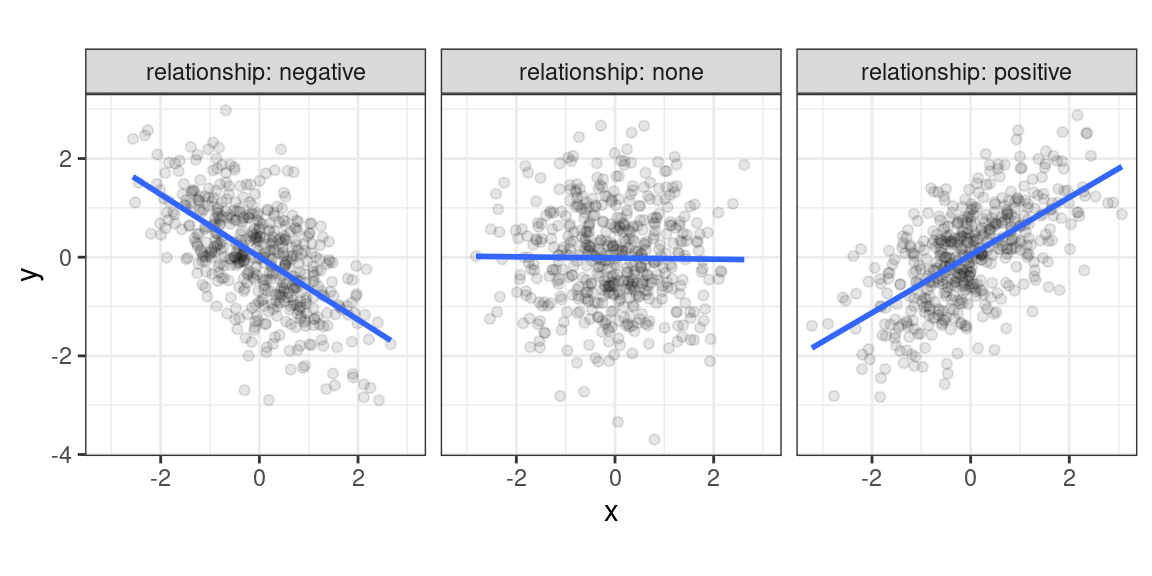
\includegraphics[width=1\linewidth]{02-bivariate-simulation_files/figure-latex/correlation-relationships-1} 

}

\caption{Different types of bivariate relationships.}\label{fig:correlation-relationships}
\end{figure}

If you have \(n\) measures, how many pairwise correlations can you compute? You can figure this out either by the formula in the info box below, or more easily you can computed it directly through the \texttt{choose(n,\ 2)} function in R. For instance, to get the number of possible pairwise correlations between 6 measures, you'd type \texttt{choose(6,\ 2)}, which tells you that you have 15 combinations.

\begin{info}
For any \(n\) measures, you can calculate \(\frac{n!}{2(n - 2)!}\)
pairwise correlations between measures. The \(!\) symbol is called the
\textbf{factorial} operator, defined as the product of all numbers from
1 to \(n\). So, if you have six measurements, you have

\[
\frac{6!}{2(6-2)!} = \frac{1 \times 2 \times 3 \times 4 \times 5 \times 6}{2\left(1 \times 2 \times 3 \times 4\right)} = \frac{720}{2(24)} = 15
\]
\end{info}

You can create a correlation matrix in R using \texttt{base::cor()} or \texttt{corrr::correlate()}. We prefer the latter function because \texttt{cor()} requires that your data is stored in a matrix, whereas most of the data we will be working with is stored in a data frame. The \texttt{corrr::correlate()} function also takes a data frame as the first argument, so it works better with pipes (\texttt{\%\textgreater{}\%}).

Let's create a correlation matrix to see how it works. Start by loading in the packages we will need.

\begin{Shaded}
\begin{Highlighting}[]
\KeywordTok{library}\NormalTok{(}\StringTok{"tidyverse"}\NormalTok{)}
\KeywordTok{library}\NormalTok{(}\StringTok{"corrr"}\NormalTok{)  }\CommentTok{# install.packages("corrr") in console if missing}
\end{Highlighting}
\end{Shaded}

We will use the \texttt{starwars} dataset, which is a built-in dataset that becomes available after you load the tidyverse package. This dataset has information about various characters that have appeared in the Star Wars film series. Let's look at the correlation between

\begin{Shaded}
\begin{Highlighting}[]
\NormalTok{starwars }\OperatorTok
\StringTok{  }\KeywordTok{select}\NormalTok{(height, mass, birth_year) }\OperatorTok
\StringTok{  }\KeywordTok{correlate}\NormalTok{()}
\end{Highlighting}
\end{Shaded}

\begin{verbatim}
## 
## Correlation method: 'pearson'
## Missing treated using: 'pairwise.complete.obs'
\end{verbatim}

\begin{verbatim}
## # A tibble: 3 x 4
##   rowname    height   mass birth_year
##   <chr>       <dbl>  <dbl>      <dbl>
## 1 height     NA      0.134     -0.400
## 2 mass        0.134 NA          0.478
## 3 birth_year -0.400  0.478     NA
\end{verbatim}

You can look up any bivariate correlation at the intersection of any given row or column. So the correlation between \texttt{height} and \texttt{mass} is .134, which you can find in row 1, column 2 or row 2, column 1; the values are the same. Note that there are only \texttt{choose(3,\ 2)} = 3 unique bivariate relationships, but each appears twice in the table. We might want to show only the unique pairs. We can do this by appending \texttt{corrr::shave()} to our pipeline.

\begin{Shaded}
\begin{Highlighting}[]
\NormalTok{starwars }\OperatorTok
\StringTok{  }\KeywordTok{select}\NormalTok{(height, mass, birth_year) }\OperatorTok
\StringTok{  }\KeywordTok{correlate}\NormalTok{() }\OperatorTok
\StringTok{  }\KeywordTok{shave}\NormalTok{()}
\end{Highlighting}
\end{Shaded}

\begin{verbatim}
## 
## Correlation method: 'pearson'
## Missing treated using: 'pairwise.complete.obs'
\end{verbatim}

\begin{verbatim}
## # A tibble: 3 x 4
##   rowname    height   mass birth_year
##   <chr>       <dbl>  <dbl>      <dbl>
## 1 height     NA     NA             NA
## 2 mass        0.134 NA             NA
## 3 birth_year -0.400  0.478         NA
\end{verbatim}

Now we've only got the lower triangle of the correlation matrix, but the \texttt{NA} values are ugly and so are the leading zeroes. The \textbf{\texttt{corrr}} package also provides the \texttt{fashion()} function that cleans things up (see \texttt{?corrr::fashion} for more options).

\begin{Shaded}
\begin{Highlighting}[]
\NormalTok{starwars }\OperatorTok
\StringTok{  }\KeywordTok{select}\NormalTok{(height, mass, birth_year) }\OperatorTok
\StringTok{  }\KeywordTok{correlate}\NormalTok{() }\OperatorTok
\StringTok{  }\KeywordTok{shave}\NormalTok{() }\OperatorTok
\StringTok{  }\KeywordTok{fashion}\NormalTok{()}
\end{Highlighting}
\end{Shaded}

\begin{verbatim}
## 
## Correlation method: 'pearson'
## Missing treated using: 'pairwise.complete.obs'
\end{verbatim}

\begin{verbatim}
##      rowname height mass birth_year
## 1     height                       
## 2       mass    .13                
## 3 birth_year   -.40  .48
\end{verbatim}

Correlations only provide a good description of the relationship if the relationship is (roughly) linear and there aren't severe outliers that are wielding too strong of an influence on the results. So it is always a good idea to visualize the correlations as well as to quantify them. The \texttt{base::pairs()} function does this. The first argument to \texttt{pairs()} is simply of the form \texttt{\textasciitilde{}\ v1\ +\ v2\ +\ v3\ +\ ...\ +\ vn} where \texttt{v1}, \texttt{v2}, etc. are the names of the variables you want to correlate.

\begin{Shaded}
\begin{Highlighting}[]
\KeywordTok{pairs}\NormalTok{(}\OperatorTok{~}\StringTok{ }\NormalTok{height }\OperatorTok{+}\StringTok{ }\NormalTok{mass }\OperatorTok{+}\StringTok{ }\NormalTok{birth_year, starwars)}
\end{Highlighting}
\end{Shaded}

\begin{figure}

{\centering \includegraphics[width=1\linewidth]{02-bivariate-simulation_files/figure-latex/pairs-1} 

}

\caption{Pairwise correlations for the starwars dataset}\label{fig:pairs}
\end{figure}

We can see that there is a big outlier influencing our data; in particular, there is a creature with a mass greater than 1200kg! Let's find out who this is and eliminate them from the dataset.

\begin{Shaded}
\begin{Highlighting}[]
\NormalTok{starwars }\OperatorTok
\StringTok{  }\KeywordTok{filter}\NormalTok{(mass }\OperatorTok{>}\StringTok{ }\DecValTok{1200}\NormalTok{) }\OperatorTok
\StringTok{  }\KeywordTok{select}\NormalTok{(name, mass, height, birth_year)}
\end{Highlighting}
\end{Shaded}

\begin{verbatim}
## # A tibble: 1 x 4
##   name                   mass height birth_year
##   <chr>                 <dbl>  <int>      <dbl>
## 1 Jabba Desilijic Tiure  1358    175        600
\end{verbatim}

OK, let's see how the data look without this massive creature.

\begin{Shaded}
\begin{Highlighting}[]
\NormalTok{starwars2 <-}\StringTok{ }\NormalTok{starwars }\OperatorTok
\StringTok{  }\KeywordTok{filter}\NormalTok{(name }\OperatorTok{!=}\StringTok{ "Jabba Desilijic Tiure"}\NormalTok{)}

\KeywordTok{pairs}\NormalTok{(}\OperatorTok{~}\NormalTok{height }\OperatorTok{+}\StringTok{ }\NormalTok{mass }\OperatorTok{+}\StringTok{ }\NormalTok{birth_year, starwars2)}
\end{Highlighting}
\end{Shaded}

\begin{figure}

{\centering 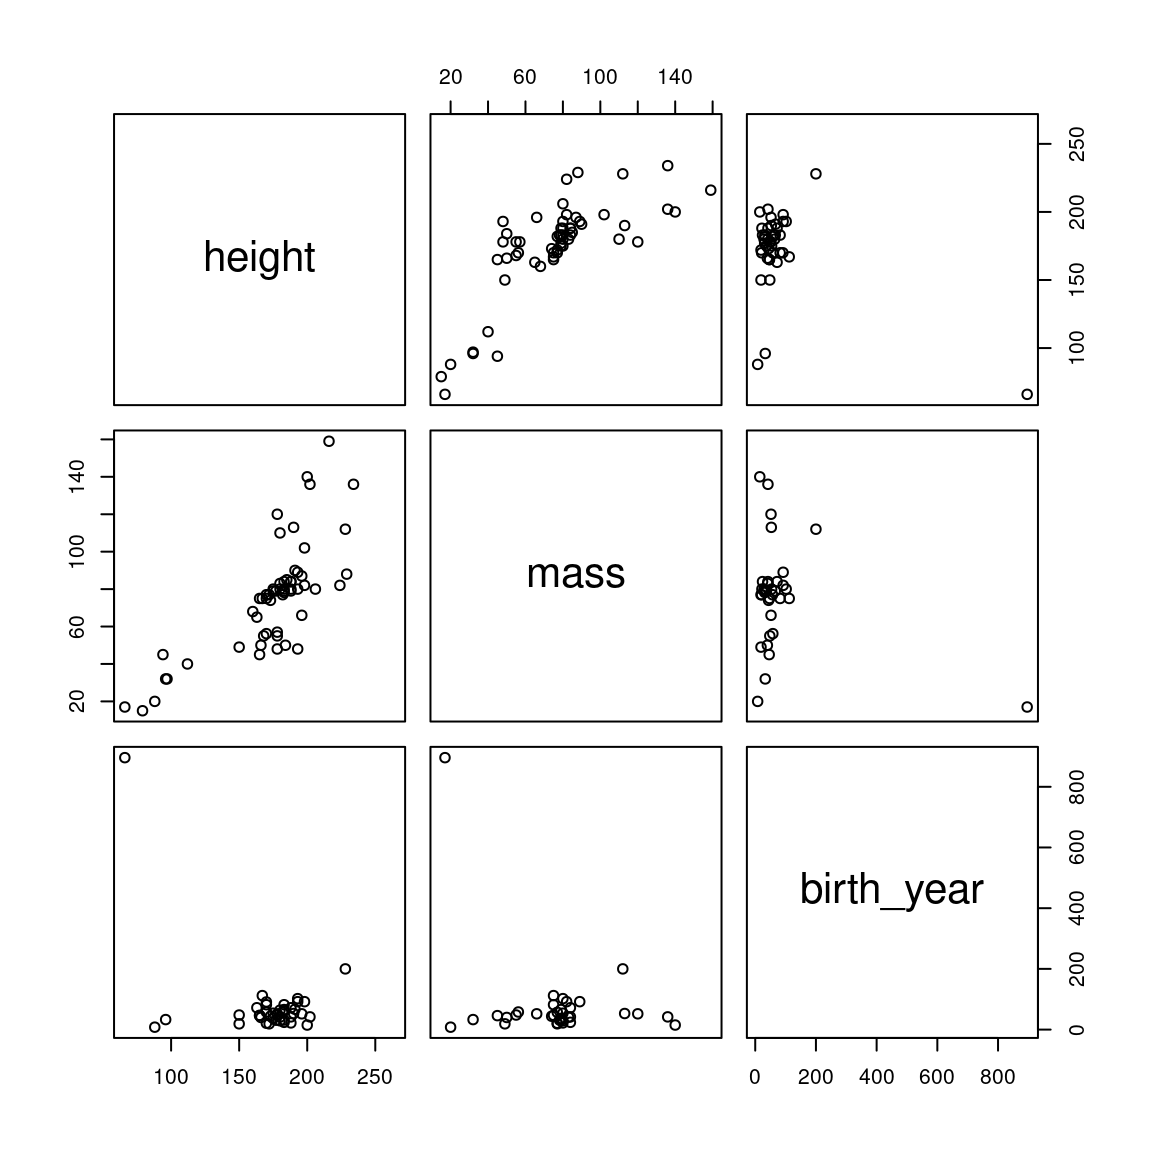
\includegraphics[width=1\linewidth]{02-bivariate-simulation_files/figure-latex/massive-creature-1} 

}

\caption{Pairwise correlations for the starwars dataset after removing outlying mass value.}\label{fig:massive-creature}
\end{figure}

Better, but there's a creature with an outlying birth year that we might want to get rid of.

\begin{Shaded}
\begin{Highlighting}[]
\NormalTok{starwars2 }\OperatorTok
\StringTok{  }\KeywordTok{filter}\NormalTok{(birth_year }\OperatorTok{>}\StringTok{ }\DecValTok{800}\NormalTok{) }\OperatorTok
\StringTok{  }\KeywordTok{select}\NormalTok{(name, height, mass, birth_year)}
\end{Highlighting}
\end{Shaded}

\begin{verbatim}
## # A tibble: 1 x 4
##   name  height  mass birth_year
##   <chr>  <int> <dbl>      <dbl>
## 1 Yoda      66    17        896
\end{verbatim}

It's Yoda. He's as old as the universe. Let's drop him and see how the plots look.

\begin{Shaded}
\begin{Highlighting}[]
\NormalTok{starwars3 <-}\StringTok{ }\NormalTok{starwars2 }\OperatorTok
\StringTok{  }\KeywordTok{filter}\NormalTok{(name }\OperatorTok{!=}\StringTok{ "Yoda"}\NormalTok{)}

\KeywordTok{pairs}\NormalTok{(}\OperatorTok{~}\NormalTok{height }\OperatorTok{+}\StringTok{ }\NormalTok{mass }\OperatorTok{+}\StringTok{ }\NormalTok{birth_year, starwars3)}
\end{Highlighting}
\end{Shaded}

\begin{figure}

{\centering 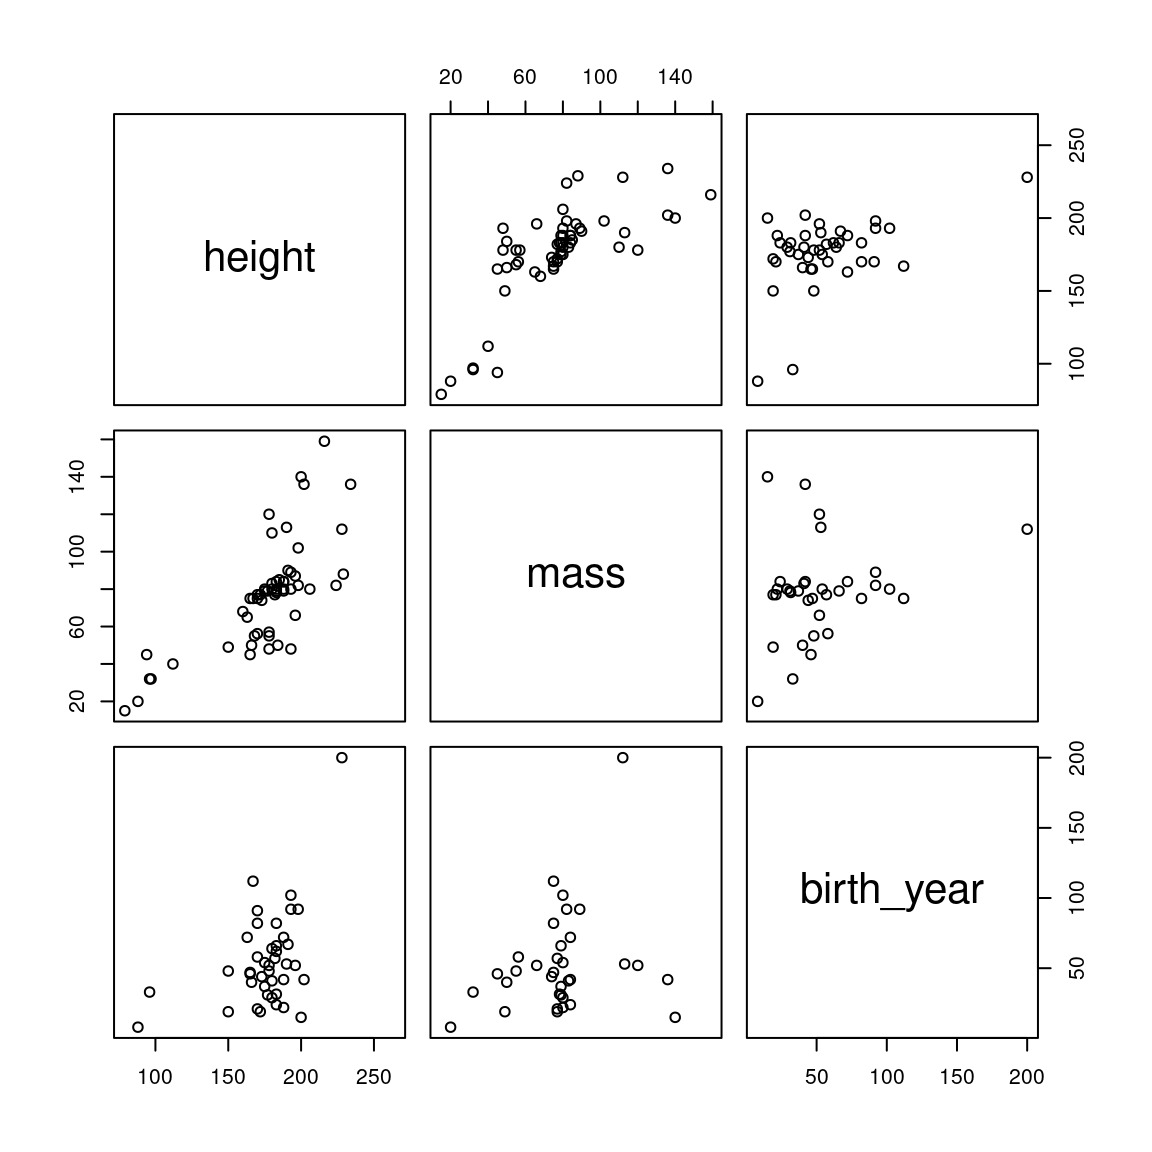
\includegraphics[width=1\linewidth]{02-bivariate-simulation_files/figure-latex/bye-yoda-1} 

}

\caption{Pairwise correlations for the starwars dataset after removing outlying mass and birth\_year values.}\label{fig:bye-yoda}
\end{figure}

That looks much better. Let's see how that changes our correlation matrix.

\begin{Shaded}
\begin{Highlighting}[]
\NormalTok{starwars3 }\OperatorTok
\StringTok{  }\KeywordTok{select}\NormalTok{(height, mass, birth_year) }\OperatorTok
\StringTok{  }\KeywordTok{correlate}\NormalTok{() }\OperatorTok
\StringTok{  }\KeywordTok{shave}\NormalTok{() }\OperatorTok
\StringTok{  }\KeywordTok{fashion}\NormalTok{()}
\end{Highlighting}
\end{Shaded}

\begin{verbatim}
## 
## Correlation method: 'pearson'
## Missing treated using: 'pairwise.complete.obs'
\end{verbatim}

\begin{verbatim}
##      rowname height mass birth_year
## 1     height                       
## 2       mass    .74                
## 3 birth_year    .45  .24
\end{verbatim}

Note that these values are quite different from the ones we started with.

Sometimes it's not a great idea to remove outliers. Another approach to dealing with outliers is to use a robust method. The default correlation coefficient that is computed by \texttt{corrr::correlate()} is the Pearson product-moment correlation coefficient. You can also compute the Spearman correlation coefficient by changing the \texttt{method()} argument to \texttt{correlate()}. This replaces the values with ranks before computing the correlation, so that outliers will still be included, but will have dramatically less influence.

\begin{Shaded}
\begin{Highlighting}[]
\NormalTok{starwars }\OperatorTok
\StringTok{  }\KeywordTok{select}\NormalTok{(height, mass, birth_year) }\OperatorTok
\StringTok{  }\KeywordTok{correlate}\NormalTok{(}\DataTypeTok{method =} \StringTok{"spearman"}\NormalTok{) }\OperatorTok
\StringTok{  }\KeywordTok{shave}\NormalTok{() }\OperatorTok
\StringTok{  }\KeywordTok{fashion}\NormalTok{()}
\end{Highlighting}
\end{Shaded}

\begin{verbatim}
## 
## Correlation method: 'spearman'
## Missing treated using: 'pairwise.complete.obs'
\end{verbatim}

\begin{verbatim}
##      rowname height mass birth_year
## 1     height                       
## 2       mass    .75                
## 3 birth_year    .16  .15
\end{verbatim}

Incidentally, if you are generating a report from R Markdown and want your tables to be nicely formatted you can use \texttt{knitr::kable()}.

\begin{Shaded}
\begin{Highlighting}[]
\NormalTok{starwars }\OperatorTok
\StringTok{  }\KeywordTok{select}\NormalTok{(height, mass, birth_year) }\OperatorTok
\StringTok{  }\KeywordTok{correlate}\NormalTok{(}\DataTypeTok{method =} \StringTok{"spearman"}\NormalTok{) }\OperatorTok
\StringTok{  }\KeywordTok{shave}\NormalTok{() }\OperatorTok
\StringTok{  }\KeywordTok{fashion}\NormalTok{() }\OperatorTok
\StringTok{  }\NormalTok{knitr}\OperatorTok{::}\KeywordTok{kable}\NormalTok{()}
\end{Highlighting}
\end{Shaded}

\begin{tabular}{l|l|l|l}
\hline
rowname & height & mass & birth\_year\\
\hline
height &  &  & \\
\hline
mass & .75 &  & \\
\hline
birth\_year & .16 & .15 & \\
\hline
\end{tabular}

\hypertarget{simulating-bivariate-data}{%
\section{Simulating bivariate data}\label{simulating-bivariate-data}}

You have already learned how to simulate data from the normal distribution using the function \texttt{rnorm()}. Recall that \texttt{rnorm()} allows you to specify the mean and standard deviation of a single variable. How do we simulate correlated variables?

It should be clear that you can't just run \texttt{rnorm()} twice and combine the variables, because then you end up with two variables that are unrelated, i.e., with a correlation of zero.

The package \textbf{\texttt{MASS}} provides a function \texttt{mvrnorm()} which is the `multivariate' version of rnorm (hence the function name, \texttt{mv} + \texttt{rnorm}, which makes it easy to remember.

\begin{watchout}
The \textbf{\texttt{MASS}} package comes pre-installed with R. But the
only function you'll probably ever want to use from
\textbf{\texttt{MASS}} is \texttt{mvrnorm()}, so rather than load in the
package using \texttt{library("MASS")}, it is preferable to use
\texttt{MASS::mvrnorm()}, especially as \textbf{\texttt{MASS}} and the
\textbf{\texttt{dplyr}} package from \textbf{\texttt{tidyverse}}
\href{https://twitter.com/dalejbarr/status/516986671129452544?s=20}{don't
play well together}, due to both packages having the function
\texttt{select()}. So if you load in \textbf{\texttt{MASS}} after you
load in \textbf{\texttt{tidyverse}}, you'll end up getting the
\textbf{\texttt{MASS}} version of \texttt{select()} instead of the
\textbf{\texttt{dplyr}} version. It will do your head in trying to
figure out what is wrong with your code, so always
\texttt{MASS::mvrnorm} and never \texttt{library("MASS")}.
\end{watchout}

Have a look at the documentation for the \texttt{mvrnorm()} function (type \texttt{?MASS::mvrnorm} in the console).

There are three arguments to take note of:

\begin{longtable}[]{@{}ll@{}}
\toprule
\begin{minipage}[b]{0.06\columnwidth}\raggedright
arg\strut
\end{minipage} & \begin{minipage}[b]{0.88\columnwidth}\raggedright
description\strut
\end{minipage}\tabularnewline
\midrule
\endhead
\begin{minipage}[t]{0.06\columnwidth}\raggedright
n\strut
\end{minipage} & \begin{minipage}[t]{0.88\columnwidth}\raggedright
the number of samples required\strut
\end{minipage}\tabularnewline
\begin{minipage}[t]{0.06\columnwidth}\raggedright
mu\strut
\end{minipage} & \begin{minipage}[t]{0.88\columnwidth}\raggedright
a vector giving the means of the variables\strut
\end{minipage}\tabularnewline
\begin{minipage}[t]{0.06\columnwidth}\raggedright
Sigma\strut
\end{minipage} & \begin{minipage}[t]{0.88\columnwidth}\raggedright
a positive-definite symmetric matrix specifying the covariance matrix of the variables.\strut
\end{minipage}\tabularnewline
\bottomrule
\end{longtable}

The descriptions for \texttt{n} and \texttt{mu} are understandable, but what is a ``positive-definite symmetric matrix specifying the covariance''?

When you have multivariate data, the \textbf{covariance matrix} (also known as the \textbf{variance-covariance} matrix) specifies the variances of the individual variables and their interrelationships. It is like a multidimensional version of the \textbf{standard deviation}. To fully describe a univariate normal distribution, you need to know only the mean and standard deviation; to describe a bivariate normal distribution, you need the means of each of the two variables, their standard deviations, and their correlation; for a multivariate distribution with more the two variables you need the means for all of the variables, their standard deviations, and all of the possible pairwise correlations. \textbf{These concepts become very important once we start talking about mixed-effects modelling.}

You can think of a covariance matrix as something like the correlation matrix that you saw above; indeed, with a few calculations you can turn a covariance matrix into a correlation matrix.

\begin{info}
What's all this talk about the Matrix? Wasn't that a sci-fi film series
from the 1990s?

In mathematics, matrices are just generalizations of the concept of a
vector: a vector can be thought of as having one dimension, whereas a
matrix can have any number of dimensions.

So the matrix

\[
\begin{pmatrix}
1 & 4 & 7 \\
2 & 5 & 8 \\
3 & 6 & 9 \\
\end{pmatrix}
\]

is a 3 (row) by 3 (column) matrix containing the column vectors
\(\begin{pmatrix} 1 \\ 2 \\ 3 \\ \end{pmatrix}\),
\(\begin{pmatrix} 4 \\ 5 \\ 6 \\ \end{pmatrix}\), and
\(\begin{pmatrix} 7 \\ 8 \\ 9 \\ \end{pmatrix}\). Conventionally, we
refer to matrices in \(i\) by \(j\) format, with \(i\) being the number
of rows and \(j\) being the number of columns. So a 3x2 matrix has 3
rows and 2 columns, like so.

\[
\begin{pmatrix}
a & d \\
b & e \\
c & f \\
\end{pmatrix}
\]

A \textbf{square matrix} is a matrix where the number of rows is equal
to the number of columns.

You can create the above matrix in R using the \texttt{matrix()}
function (see below) or by binding together vectors column-wise, using
the base R \texttt{cbind()} function. Try
\texttt{cbind(1:3,\ 4:6,\ 7:9)} in your console. You can also bind
vectors together row-wise using \texttt{rbind()}.
\end{info}

Now what is all this about the matrix being ``positive-definite'' and ``symmetric''? These are mathematical requirements about the kinds of matrices that can represent possible multivariate normal distributions. In other words, the covariance matrix you supply must be represent a legal multivariate normal distribution. At this point, you don't really need to know much more about this than that.

Let's start by simulating data representing hypothetical humans and their heights and weights. We know these things are correlated. What we need to be able to simulate data are means and standard deviations for these two variables and their correlation.

I found some data \href{https://www.geogebra.org/m/RRprACv4}{here} which I converted into a CSV file. If you want to follow along, download the file \href{data/heights_and_weights.csv}{heights\_and\_weights.csv}. Here's how the scatterplot looks:

\begin{Shaded}
\begin{Highlighting}[]
\NormalTok{handw <-}\StringTok{ }\KeywordTok{read_csv}\NormalTok{(}\StringTok{"data/heights_and_weights.csv"}\NormalTok{, }\DataTypeTok{col_types =} \StringTok{"dd"}\NormalTok{)}

\KeywordTok{ggplot}\NormalTok{(handw, }\KeywordTok{aes}\NormalTok{(height_in, weight_lbs)) }\OperatorTok{+}\StringTok{ }
\StringTok{  }\KeywordTok{geom_point}\NormalTok{(}\DataTypeTok{alpha =} \FloatTok{.2}\NormalTok{) }\OperatorTok{+}
\StringTok{  }\KeywordTok{labs}\NormalTok{(}\DataTypeTok{x =} \StringTok{"height (inches)"}\NormalTok{, }\DataTypeTok{y =} \StringTok{"weight (pounds)"}\NormalTok{) }
\end{Highlighting}
\end{Shaded}

\begin{figure}

{\centering 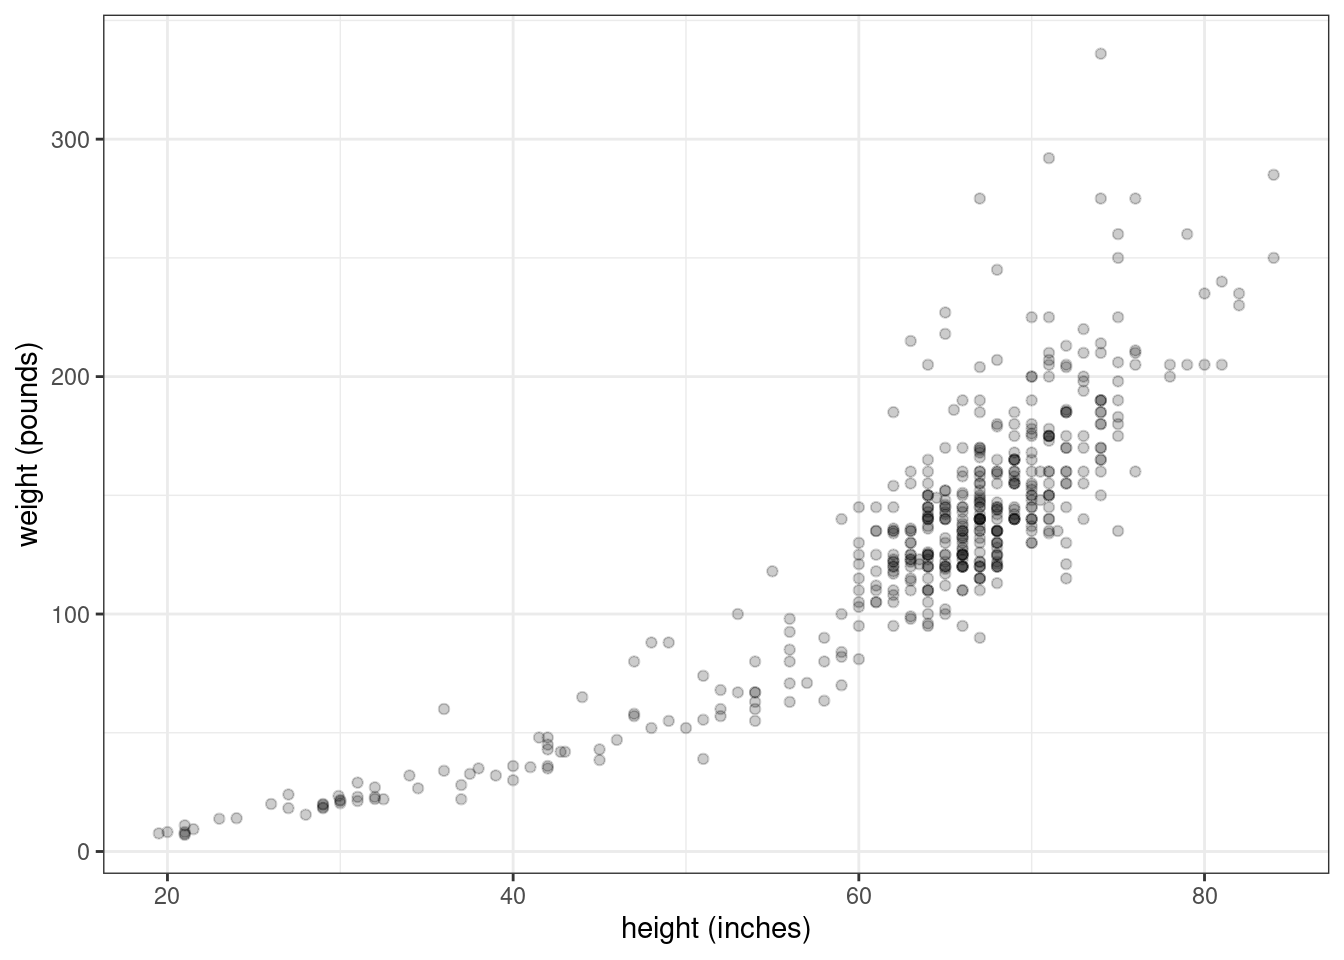
\includegraphics[width=1\linewidth]{02-bivariate-simulation_files/figure-latex/heights-and-weights-1} 

}

\caption{Heights and weights of 475 humans (including infants)}\label{fig:heights-and-weights}
\end{figure}

Now, that's not quite a linear relationship. We can make it into one by log transforming each of the variables first.

\begin{Shaded}
\begin{Highlighting}[]
\NormalTok{handw_log <-}\StringTok{ }\NormalTok{handw }\OperatorTok
\StringTok{  }\KeywordTok{mutate}\NormalTok{(}\DataTypeTok{hlog =} \KeywordTok{log}\NormalTok{(height_in),}
         \DataTypeTok{wlog =} \KeywordTok{log}\NormalTok{(weight_lbs))}
\end{Highlighting}
\end{Shaded}

\begin{figure}

{\centering 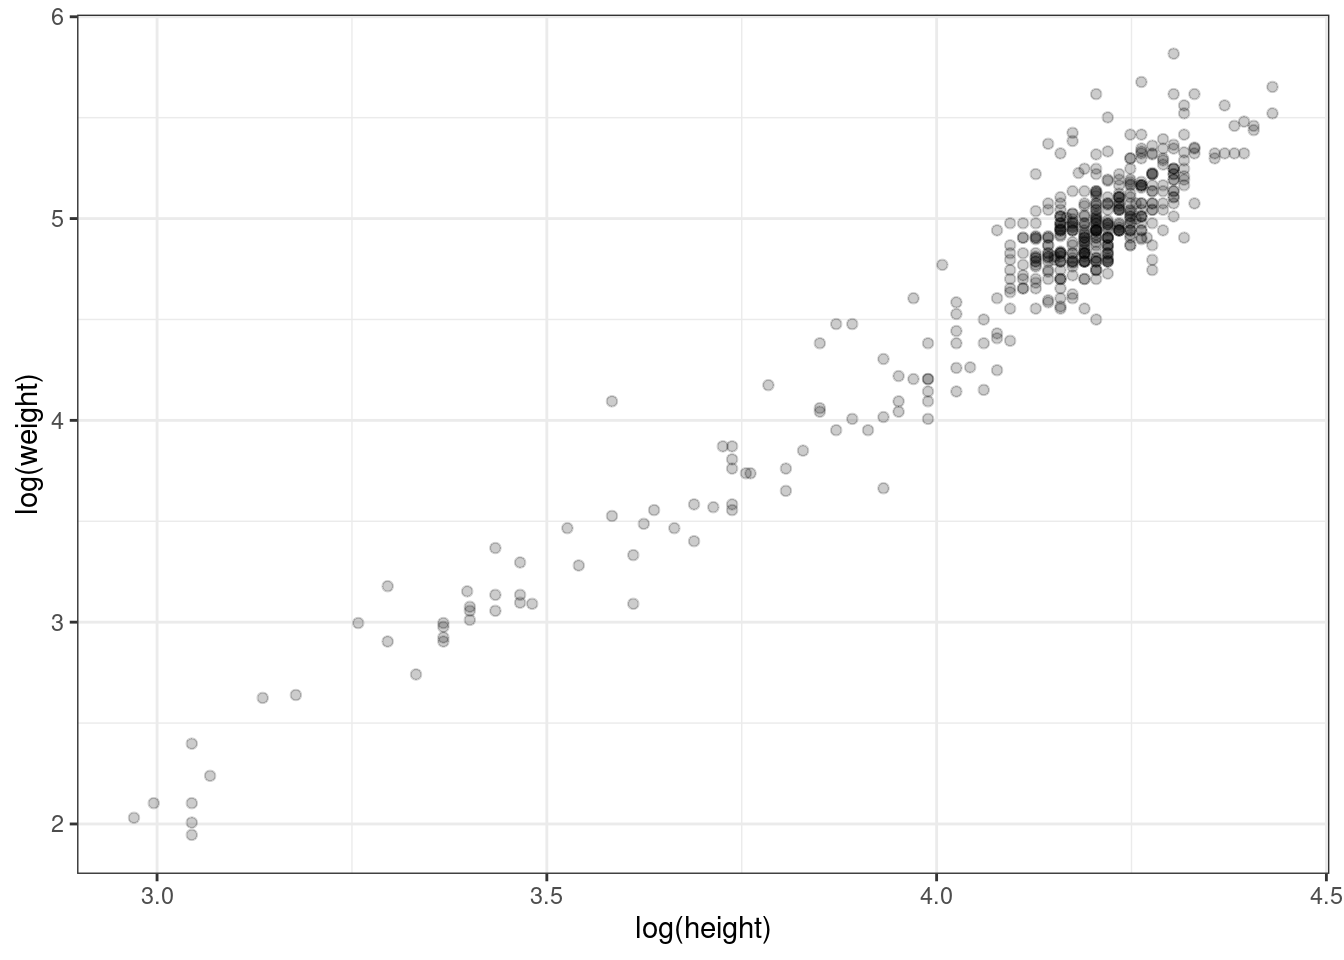
\includegraphics[width=1\linewidth]{02-bivariate-simulation_files/figure-latex/handw-log-1} 

}

\caption{Log transformed heights and weights.}\label{fig:handw-log}
\end{figure}

The fact that there is a big cluster of points in the top right tail of the cloud probably indicates that there were more adults than kids in this sample, since adults are taller and heavier.

The mean log height is 4.11 (SD = 0.26), while the mean log weight is 4.74 (SD = 0.65). The correlation between log height and log weight, which we can get using the \texttt{cor()} function, is very high, 0.96.

We now have all the information we need to simulate the heights and weights of, let's say, 500 humans. But how do we get this information into \texttt{MASS::mvrnorm()}? We know the first part of the function call will be \texttt{MASS::mvrnorm(500,\ c(4.11,\ 4.74),\ ...)}, but what about \texttt{Sigma}, the covariance matrix? We know from above that \(\hat{\sigma}_x = 0.26\) and \(\hat{\sigma}_y = 0.65\), and \(\hat{\rho}_{xy} = 0.96\).

A covariance matrix representating \texttt{Sigma} (\(\mathbf{\Sigma}\)) for bivariate data has the following format:

\[
\mathbf{\Sigma} =
\begin{pmatrix}
{\sigma_x}^2                & \rho_{xy} \sigma_x \sigma_y \\
\rho_{yx} \sigma_y \sigma_x & {\sigma_y}^2 \\
\end{pmatrix}
\]

The variances (squared standard deviations, \({\sigma_x}^2\) and \({\sigma_y}^2\)) are in the diagonal, and the covariances (the correlation times the two standard deviations, \(\rho_{xy} \sigma_x \sigma_y\)) are in the off-diagonal. It is useful to remember that the covariance is just the correlation times the product of the two standard deviations. As we saw above with the correlation matrices, there is redundant information in the table; namely, the covariance appears in the top right cell as well as the bottom left cell of the matrix.

So plugging in the values we got above, our covariance matrix should be

\[
\begin{pmatrix}
.26^2 & (.96)(.26)(.65) \\
(.96)(.65)(.26) & .65^2 \\
\end{pmatrix} =
\begin{pmatrix}
.067 & .162 \\
.162 & .423 \\
\end{pmatrix}
\]

OK, how do we form \texttt{Sigma} in R so that we can pass it to the \texttt{mvrnorm()} function? We will use the \texttt{matrix()} function, as shown below.

First let's define our covariance and store it in the variable \texttt{my\_cov}.

\begin{Shaded}
\begin{Highlighting}[]
\NormalTok{my_cov <-}\StringTok{ }\FloatTok{.96} \OperatorTok{*}\StringTok{ }\FloatTok{.26} \OperatorTok{*}\StringTok{ }\FloatTok{.65}
\end{Highlighting}
\end{Shaded}

Now we'll use \texttt{matrix()} to define our \texttt{Sigma}, \texttt{my\_Sigma}.

\begin{Shaded}
\begin{Highlighting}[]
\NormalTok{my_Sigma <-}\StringTok{ }\KeywordTok{matrix}\NormalTok{(}\KeywordTok{c}\NormalTok{(.}\DecValTok{26}\OperatorTok{^}\DecValTok{2}\NormalTok{, my_cov, my_cov, }\FloatTok{.65}\OperatorTok{^}\DecValTok{2}\NormalTok{), }\DataTypeTok{ncol =} \DecValTok{2}\NormalTok{)}
\NormalTok{my_Sigma}
\end{Highlighting}
\end{Shaded}

\begin{verbatim}
##         [,1]    [,2]
## [1,] 0.06760 0.16224
## [2,] 0.16224 0.42250
\end{verbatim}

\begin{info}
Confused about the \texttt{matrix()} function?

The first argument is a vector of values, which we created above using
\texttt{c()}. The \texttt{ncol} argument specifies how many columns the
matrix should have. There is also an \texttt{nrow} argument that you
could use, but if you give it one of the dimensions, it can infer the
size of the other using the length of the vector supplied as the first
argument.

You can see that \texttt{matrix()} fills in the elements of the matrix
column by column, rather than row by row by running the following code:

\texttt{matrix(c("a",\ "b",\ "c",\ "d"),\ ncol\ =\ 2)}

If you want to change this behavior, set the \texttt{byrow} argument to
\texttt{TRUE}.

\texttt{matrix(c("a",\ "b",\ "c",\ "d"),\ ncol\ =\ 2,\ byrow\ =\ TRUE)}
\end{info}

Great. Now that we've got \texttt{my\_Sigma}, we're ready to use \texttt{MASS::mvrnorm()}. Let's test it out by creating 6 synthetic humans.

\begin{Shaded}
\begin{Highlighting}[]
\KeywordTok{set.seed}\NormalTok{(}\DecValTok{62}\NormalTok{) }\CommentTok{# for reproducibility}

\CommentTok{# passing the *named* vector c(height = 4.11, weight = 4.74)}
\CommentTok{# for mu gives us column names in the output}
\NormalTok{log_ht_wt <-}\StringTok{ }\NormalTok{MASS}\OperatorTok{::}\KeywordTok{mvrnorm}\NormalTok{(}\DecValTok{6}\NormalTok{, }
                           \KeywordTok{c}\NormalTok{(}\DataTypeTok{height =} \FloatTok{4.11}\NormalTok{, }\DataTypeTok{weight =} \FloatTok{4.74}\NormalTok{), }
\NormalTok{                           my_Sigma)}

\NormalTok{log_ht_wt}
\end{Highlighting}
\end{Shaded}

\begin{verbatim}
##        height   weight
## [1,] 4.254209 5.282913
## [2,] 4.257828 4.895222
## [3,] 3.722376 3.759767
## [4,] 4.191287 4.764229
## [5,] 4.739967 6.185191
## [6,] 4.058105 4.806485
\end{verbatim}

So \texttt{MASS::mvrnorm()} returns a matrix with a row for each simulated human, with the first column representing the log height and the second column representing the log weight. But log heights and log weights are not very useful to us, so let's transform them back by using \texttt{exp()}, which is the inverse of the \texttt{log()} transform.

\begin{Shaded}
\begin{Highlighting}[]
\KeywordTok{exp}\NormalTok{(log_ht_wt)}
\end{Highlighting}
\end{Shaded}

\begin{verbatim}
##         height    weight
## [1,]  70.40108 196.94276
## [2,]  70.65632 133.64963
## [3,]  41.36254  42.93844
## [4,]  66.10779 117.24065
## [5,] 114.43045 485.50576
## [6,]  57.86453 122.30092
\end{verbatim}

So our first simulated human is 70.4 inches tall (about 5'5" or X) and weighs 196.94 pounds (89.32 kg). Sounds about right! (Note also that it will generate observations outside of our original data; we'll get super tall humans, like observation 5, but at least the weight/height relationship will be preserved.)

OK, let's randomly generate a bunch of humans, transform them from log to inches and pounds, and plot them against our original data to see how we're doing.

\begin{Shaded}
\begin{Highlighting}[]
\CommentTok{## simulate new humans}
\NormalTok{new_humans <-}\StringTok{ }\NormalTok{MASS}\OperatorTok{::}\KeywordTok{mvrnorm}\NormalTok{(}\DecValTok{500}\NormalTok{, }
                            \KeywordTok{c}\NormalTok{(}\DataTypeTok{height_in =} \FloatTok{4.11}\NormalTok{, }\DataTypeTok{weight_lbs =} \FloatTok{4.74}\NormalTok{),}
\NormalTok{                            my_Sigma) }\OperatorTok
\StringTok{  }\KeywordTok{exp}\NormalTok{() }\OperatorTok\StringTok{ }\CommentTok{# back-transform from log to inches and pounds}
\StringTok{  }\KeywordTok{as_tibble}\NormalTok{() }\OperatorTok\StringTok{ }\CommentTok{# make tibble for plotting}
\StringTok{  }\KeywordTok{mutate}\NormalTok{(}\DataTypeTok{type =} \StringTok{"simulated"}\NormalTok{) }\CommentTok{# tag them as simulated}

\CommentTok{## combine real and simulated datasets}
\CommentTok{## handw is variable containing data from heights_and_weights.csv}
\NormalTok{alldata <-}\StringTok{ }\KeywordTok{bind_rows}\NormalTok{(handw }\OperatorTok\StringTok{ }\KeywordTok{mutate}\NormalTok{(}\DataTypeTok{type =} \StringTok{"real"}\NormalTok{), }
\NormalTok{                     new_humans)}

\KeywordTok{ggplot}\NormalTok{(alldata, }\KeywordTok{aes}\NormalTok{(height_in, weight_lbs)) }\OperatorTok{+}
\StringTok{  }\KeywordTok{geom_point}\NormalTok{(}\KeywordTok{aes}\NormalTok{(}\DataTypeTok{colour =}\NormalTok{ type), }\DataTypeTok{alpha =} \FloatTok{.1}\NormalTok{)}
\end{Highlighting}
\end{Shaded}

\begin{figure}

{\centering 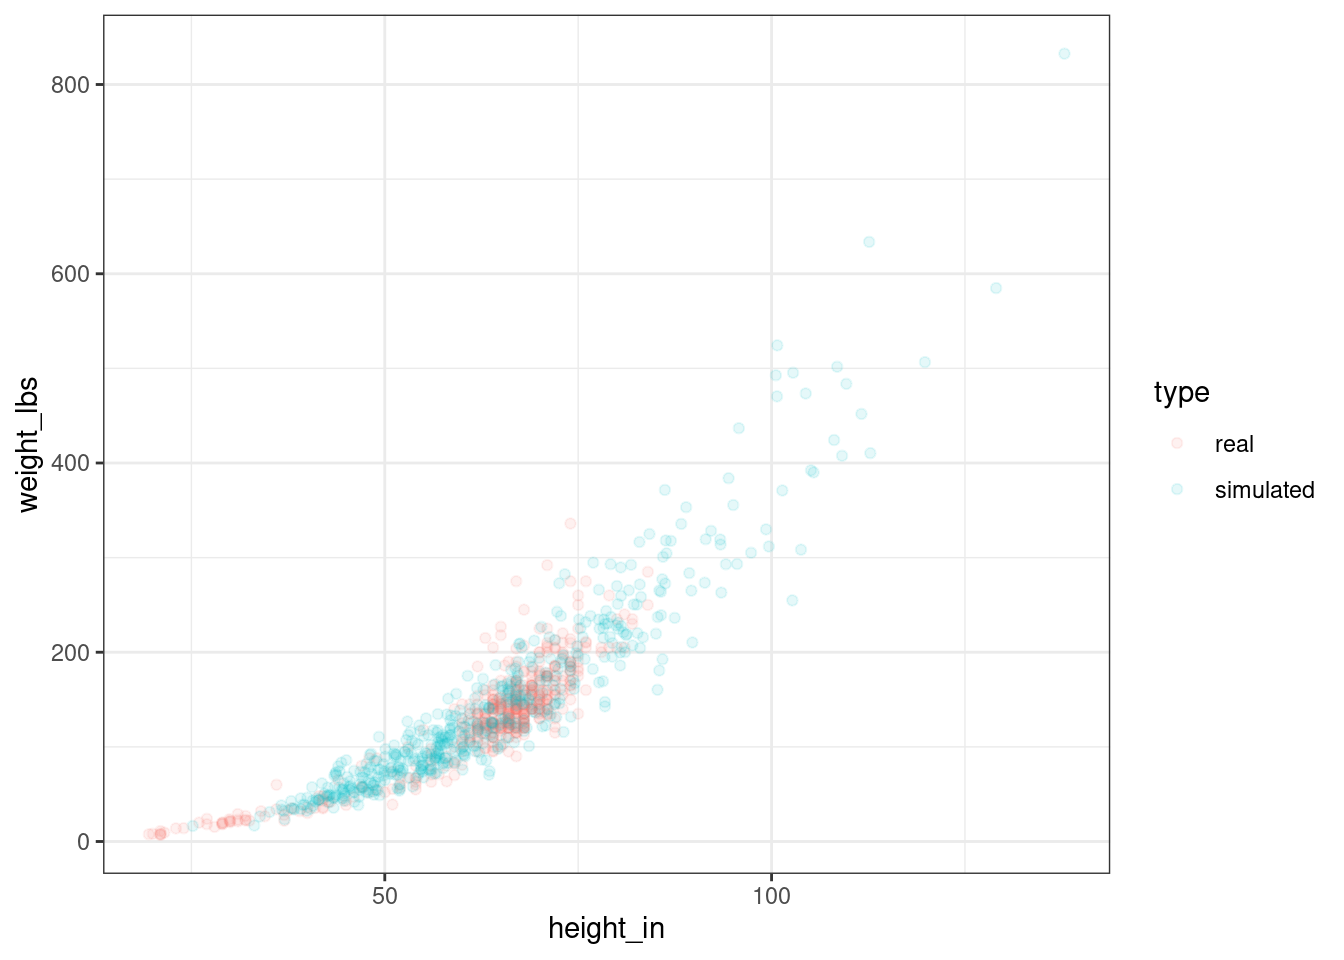
\includegraphics[width=1\linewidth]{02-bivariate-simulation_files/figure-latex/plot-together-1} 

}

\caption{Real and simulated humans.}\label{fig:plot-together}
\end{figure}

You can see that our simulated humans are much like the normal ones, except that we are creating humans outside the normal range of heights and weights.

\hypertarget{bivariate-app}{%
\subsection{Bivariate app}\label{bivariate-app}}

Here is a web app that you should play around with to better understand the relationship between covariance matrices, bivariate normal distributions, and correlation coefficients.

\hypertarget{relationship-between-correlation-and-regression}{%
\section{Relationship between correlation and regression}\label{relationship-between-correlation-and-regression}}

OK, we know how to estimate correlations, but what if we wanted to predict the weight of someone given their height? This might sound like an impractical problem, but in fact, \href{https://link.springer.com/article/10.1186/s12245-018-0212-9}{emergency medical technicians can use this technique to get a quick estimate of people's weights in emergency situations} where they need to administer drugs or procedures whose safety depends on the patient's weight, and don't have time to weigh them.

Recall that the GLM for a simple regression model is

\[Y_i = \beta_0 + \beta_1 X_i + e_i.\]

Here, we are trying to predict the weight (\(Y_i\)) of person \(i\) from their observed height (\(X_i\)). In this equation, \(\beta_0\) and \(\beta_1\) are the y-intercept and slope parameters respectively, and the \(e_i\)s are the residuals. It is conventionally assumed that the \(e_i\) values are from a normal distribution with mean of zero and variance \(\sigma^2\); the math-y way of saying this is \(e_i \sim N(0, \sigma^2)\), where \(\sim\) is read as ``distributed according to'' and \(N(0, \sigma^2)\) means ``Normal distribution (\(N\)) with mean of 0 and variance of \(\sigma^2\)''.

It turns out that if we have estimates of the means of X and Y (denoted by \(\mu_x\) and \(\mu_y\) respectively), of their standard deviations (\(\hat{\sigma}_x\) and \(\hat{\sigma}_y\)), and the correlation between X and Y (\(\hat{\rho}\)), we have all the information we need to estimate the parameters of the regression equation \(\beta_0\) and \(\beta_1\). Here's how.

First, the slope of the regression line \(\beta_1\) equals the correlation coefficient \(\rho\) times the ratio of the standard deviations of \(Y\) and \(X\).

\[\beta_1 = \rho \frac{\sigma_Y}{\sigma_X}\]

Given the estimates above for log height and weight, can you solve for \(\beta_1\)?

\begin{Shaded}
\begin{Highlighting}[]
\NormalTok{b1 <-}\StringTok{ }\FloatTok{.96} \OperatorTok{*}\StringTok{ }\NormalTok{(.}\DecValTok{65} \OperatorTok{/}\StringTok{ }\FloatTok{.26}\NormalTok{)}
\NormalTok{b1}
\end{Highlighting}
\end{Shaded}

\begin{verbatim}
## [1] 2.4
\end{verbatim}

The next thing to note is that for mathematical reasons, the regression line is guaranteed to go through the point corresponding to the mean of \(X\) and the mean of \(Y\), i.e., the point \((\mu_x, \mu_y)\). (You can think of the regression line ``pivoting'' around that point depending on the slope). You also know that \(\beta_0\) is the y-intercept, the point where the line crosses the vertical axis at \(X = 0\). From this information, and the estimates above, can you figure out the value of \(\beta_0\)?

Here is the reasoning by which you can solve for \(\beta_0\).

The \(\beta_1\) value tells you that for each change in \(X\) you have a corresponding change of 2.4 for \(Y\), and you know that the line goes through the points \((\mu_x, \mu_y)\) as well as the y-intercept \((0, \beta_0)\).

Think about stepping back unit-by-unit from \(X = \mu_x\) to \(X = 0\).
At \(X = \mu_x\), \(Y = 4.74\). Each unit step you take backward in the X dimension, \(Y\) will drop by \(\beta_1 = 2.4\) units. When you get to zero, \(Y\) will have dropped from \(\mu_y\) to \(\mu_y - \mu_x\beta_1\).

So the general solution is: \(\beta_0 = \mu_y - \mu_x\beta_1\).

Since \(\beta_1 = 2.4\), \(\mu_x = 4.11\), and \(\mu_y = 4.74\), \(\beta_0 = -5.124\). Thus, our regression equation is:

\[Y_i =  -5.124 + 2.4X_i + e_i.\]

To check our results, let's first run a regression on the log-transformed data using \texttt{lm()}, which estimates parameters using ordinary least squares regression.

\begin{Shaded}
\begin{Highlighting}[]
\KeywordTok{summary}\NormalTok{(}\KeywordTok{lm}\NormalTok{(wlog }\OperatorTok{~}\StringTok{ }\NormalTok{hlog, handw_log))}
\end{Highlighting}
\end{Shaded}

\begin{verbatim}
## 
## Call:
## lm(formula = wlog ~ hlog, data = handw_log)
## 
## Residuals:
##      Min       1Q   Median       3Q      Max 
## -0.63296 -0.09915 -0.01366  0.09285  0.65635 
## 
## Coefficients:
##             Estimate Std. Error t value Pr(>|t|)    
## (Intercept) -5.26977    0.13169  -40.02   <2e-16 ***
## hlog         2.43304    0.03194   76.17   <2e-16 ***
## ---
## Signif. codes:  0 '***' 0.001 '**' 0.01 '*' 0.05 '.' 0.1 ' ' 1
## 
## Residual standard error: 0.1774 on 473 degrees of freedom
## Multiple R-squared:  0.9246,	Adjusted R-squared:  0.9245 
## F-statistic:  5802 on 1 and 473 DF,  p-value: < 2.2e-16
\end{verbatim}

Looks pretty close. The reason that it doesn't match exactly is only because we've rounded off our estimates to two decimal places for convenience.

As another check, let's superimpose the regression line we computed by hand on the scatterplot of the log-transformed data.

\begin{Shaded}
\begin{Highlighting}[]
\KeywordTok{ggplot}\NormalTok{(handw_log, }\KeywordTok{aes}\NormalTok{(hlog, wlog)) }\OperatorTok{+}
\StringTok{  }\KeywordTok{geom_point}\NormalTok{(}\DataTypeTok{alpha =} \FloatTok{.2}\NormalTok{) }\OperatorTok{+}
\StringTok{  }\KeywordTok{labs}\NormalTok{(}\DataTypeTok{x =} \StringTok{"log(height)"}\NormalTok{, }\DataTypeTok{y =} \StringTok{"log(weight)"}\NormalTok{) }\OperatorTok{+}
\StringTok{  }\KeywordTok{geom_abline}\NormalTok{(}\DataTypeTok{intercept =} \FloatTok{-5.124}\NormalTok{, }\DataTypeTok{slope =} \FloatTok{2.4}\NormalTok{, }\DataTypeTok{colour =} \StringTok{'blue'}\NormalTok{)}
\end{Highlighting}
\end{Shaded}

\begin{figure}

{\centering 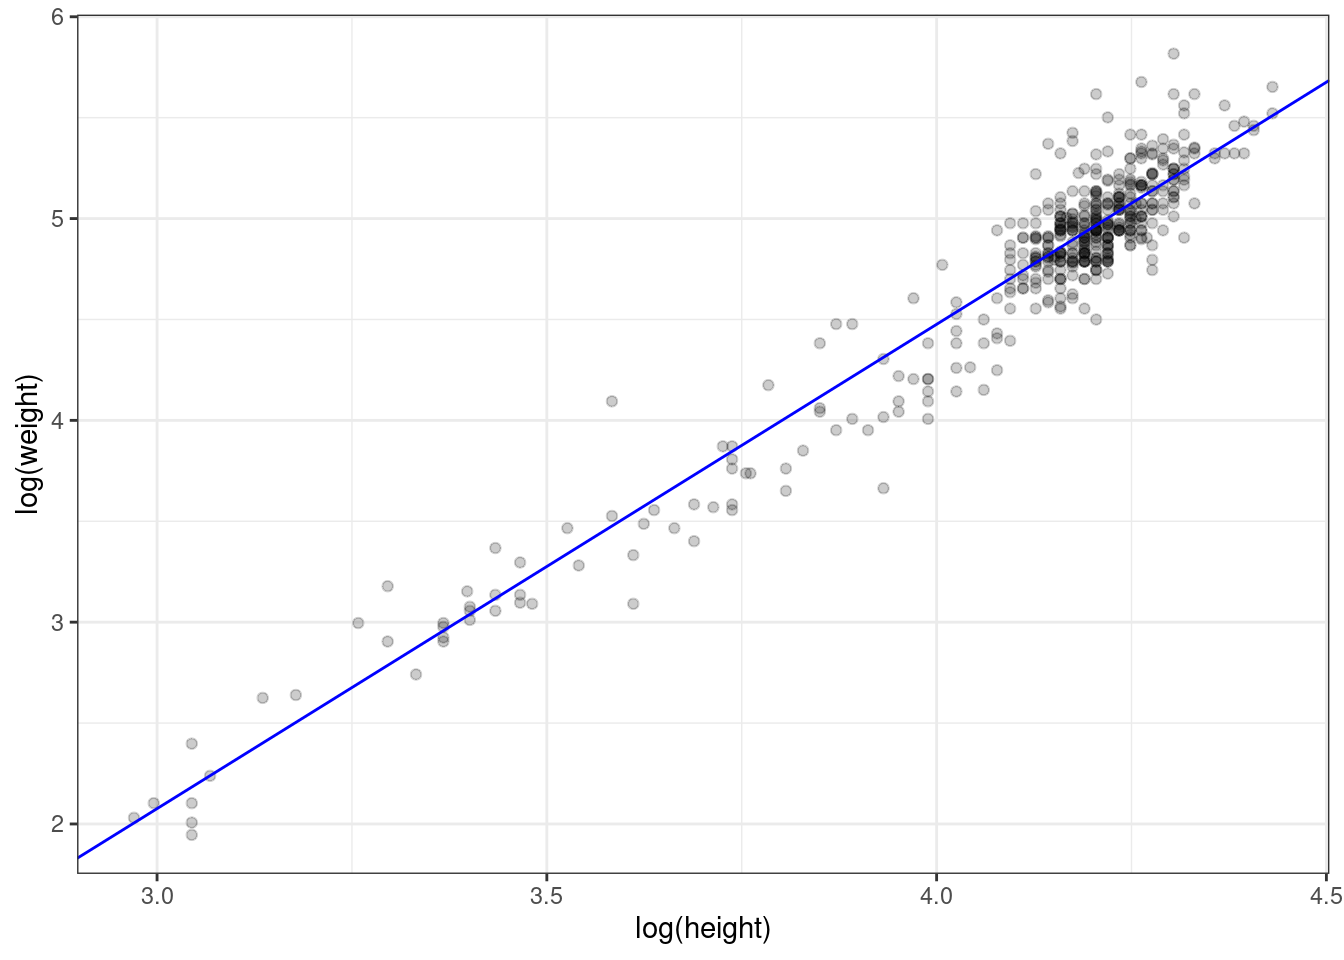
\includegraphics[width=1\linewidth]{02-bivariate-simulation_files/figure-latex/scatter-with-line-1} 

}

\caption{Log transformed values with superimposed regression line.}\label{fig:scatter-with-line}
\end{figure}

Looks right.

To close, here are a few implications from the relationship between correlation and regression.

\begin{itemize}
\tightlist
\item
  \(\beta_1 = 0\) is the same as \(\rho = 0\).
\item
  \(\beta_1 > 0\) implies \(\rho > 0\), since standard deviations can't be negative.
\item
  \(\beta_1 < 0\) implies \(\rho < 0\), for the same reason.
\item
  Rejecting the null hypothesis that \(\beta_1 = 0\) is the same as rejecting the null hypothesis that \(\rho = 0\). The p-values that you get for \(\beta_1\) in \texttt{lm()} will be the same as the one you get for \(\rho\) from \texttt{cor.test()}.
\end{itemize}

\hypertarget{multiple-regression}{%
\chapter{Multiple regression}\label{multiple-regression}}

General model for single-level data with \(m\) predictors:

\[
Y_i = \beta_0 + \beta_1 X_{1i} + \beta_2 X_{2i} + \ldots + \beta_m X_{mi} + e_i
\]

The individual \(X_{hi}\) variables can be any combination of continuous and/or categorical predictors, including interactions among variables.

The \(\beta\) values are referred to as \textbf{regression coefficients}. Each \(\beta_h\) is interpreted as the \textbf{partial effect of \(\beta_h\) holding constant all other predictor variables.} If you have \(m\) predictor variables, you have \(m+1\) regression coefficients: one for the intercept, and one for each predictor.

Although discussions of multiple regression are common in statistical textbooks, you will rarely be able to apply the exact model above. This is because the above model assumes single-level data, whereas most psychological data is multi-level. However, the fundamentals are the same for both types of datasets, so it is worthwhile learning them for the simpler case first.

\hypertarget{an-example-how-to-get-a-good-grade-in-statistics}{%
\section{An example: How to get a good grade in statistics}\label{an-example-how-to-get-a-good-grade-in-statistics}}

Let's look at some (made up, but realistic) data to see how we can use multiple regression to answer various study questions. In this hypothetical study, you have a dataset for 100 statistics students, which includes their final course grade (\texttt{grade}), the number of lectures each student attended (\texttt{lecture}, an integer ranging from 0-10), how many times each student clicked to download online materials (\texttt{nclicks}) and each student's grade point average prior to taking the course, \texttt{GPA}, which ranges from 0 (fail) to 4 (highest possible grade).

\hypertarget{data-import-and-visualization}{%
\subsection{Data import and visualization}\label{data-import-and-visualization}}

Let's load in the data \href{data/grades.csv}{grades.csv} and have a look.

\begin{Shaded}
\begin{Highlighting}[]
\KeywordTok{library}\NormalTok{(}\StringTok{"corrr"}\NormalTok{) }\CommentTok{# correlation matrices}
\KeywordTok{library}\NormalTok{(}\StringTok{"tidyverse"}\NormalTok{)}

\NormalTok{grades <-}\StringTok{ }\KeywordTok{read_csv}\NormalTok{(}\StringTok{"data/grades.csv"}\NormalTok{, }\DataTypeTok{col_types =} \StringTok{"ddii"}\NormalTok{)}

\NormalTok{grades}
\end{Highlighting}
\end{Shaded}

\begin{verbatim}
## # A tibble: 100 x 4
##    grade   GPA lecture nclicks
##    <dbl> <dbl>   <int>   <int>
##  1  2.40 1.13        6      88
##  2  3.67 0.971       6      96
##  3  2.85 3.34        6     123
##  4  1.36 2.76        9      99
##  5  2.31 1.02        4      66
##  6  2.58 0.841       8      99
##  7  2.69 4           5      86
##  8  3.05 2.29        7     118
##  9  3.21 3.39        9      98
## 10  2.24 3.27       10     115
## # ... with 90 more rows
\end{verbatim}

First let's look at all the pairwise correlations.

\begin{Shaded}
\begin{Highlighting}[]
\NormalTok{grades }\OperatorTok
\StringTok{  }\KeywordTok{correlate}\NormalTok{() }\OperatorTok
\StringTok{  }\KeywordTok{shave}\NormalTok{() }\OperatorTok
\StringTok{  }\KeywordTok{fashion}\NormalTok{()}
\end{Highlighting}
\end{Shaded}

\begin{verbatim}
## 
## Correlation method: 'pearson'
## Missing treated using: 'pairwise.complete.obs'
\end{verbatim}

\begin{verbatim}
##   rowname grade  GPA lecture nclicks
## 1   grade                           
## 2     GPA   .25                     
## 3 lecture   .24  .44                
## 4 nclicks   .16  .30     .36
\end{verbatim}

\begin{Shaded}
\begin{Highlighting}[]
\KeywordTok{pairs}\NormalTok{(grades)}
\end{Highlighting}
\end{Shaded}

\begin{figure}

{\centering \includegraphics[width=1\linewidth]{03-multiple-regression_files/figure-latex/pairs-1} 

}

\caption{All pairwise relationships in the `grades` dataset.}\label{fig:pairs}
\end{figure}

\hypertarget{estimation-and-interpretation}{%
\subsection{Estimation and interpretation}\label{estimation-and-interpretation}}

To estimate the regression coefficients (the \(\beta\)s), we will use the \texttt{lm()} function. For a GLM with \(m\) predictors:

\[
Y_i = \beta_0 + \beta_1 X_{1i} + \beta_2 X_{2i} + \ldots + \beta_m X_{mi} + e_i
\]

The call to base R's \texttt{lm()} is

\texttt{lm(Y\ \textasciitilde{}\ X1\ +\ X2\ +\ ...\ +\ Xm,\ data)}

The \texttt{Y} variable is your response variable, and the \texttt{X} variables are the predictor variables. Note that you don't need to explicitly specify the intercept or residual terms; those are included by default.

For the current data, let's predict \texttt{grade} from \texttt{lecture} and \texttt{nclicks}.

\begin{Shaded}
\begin{Highlighting}[]
\NormalTok{my_model <-}\StringTok{ }\KeywordTok{lm}\NormalTok{(grade }\OperatorTok{~}\StringTok{ }\NormalTok{lecture }\OperatorTok{+}\StringTok{ }\NormalTok{nclicks, grades)}

\KeywordTok{summary}\NormalTok{(my_model)}
\end{Highlighting}
\end{Shaded}

\begin{verbatim}
## 
## Call:
## lm(formula = grade ~ lecture + nclicks, data = grades)
## 
## Residuals:
##      Min       1Q   Median       3Q      Max 
## -2.21653 -0.40603  0.02267  0.60720  1.38558 
## 
## Coefficients:
##             Estimate Std. Error t value Pr(>|t|)  
## (Intercept) 1.462037   0.571124   2.560   0.0120 *
## lecture     0.091501   0.045766   1.999   0.0484 *
## nclicks     0.005052   0.006051   0.835   0.4058  
## ---
## Signif. codes:  0 '***' 0.001 '**' 0.01 '*' 0.05 '.' 0.1 ' ' 1
## 
## Residual standard error: 0.8692 on 97 degrees of freedom
## Multiple R-squared:  0.06543,	Adjusted R-squared:  0.04616 
## F-statistic: 3.395 on 2 and 97 DF,  p-value: 0.03756
\end{verbatim}

We'll often write the parameter symbol with a little hat on top to make clear that we are dealing with estimates from the sample rather than the (unknown) true population values. From above:

\begin{itemize}
\tightlist
\item
  \(\hat{\beta}_0\) = 1.46
\item
  \(\hat{\beta}_1\) = 0.09
\item
  \(\hat{\beta}_2\) = 0.01
\end{itemize}

This tells us that a person's predicted grade is related to their lecture attendance and download rate by the following formula:

\texttt{grade} = 1.46 + 0.09 \(\times\) \texttt{lecture} + 0.01 \(\times\) \texttt{nclicks}

Because \(\hat{\beta}_1\) and \(\hat{\beta}_2\) are both positive, we know that higher values of \texttt{lecture} and \texttt{nclicks} are associated with higher grades.

So if you were asked, what grade would you predict for a student who attends 3 lectures and downloaded 70 times, you could easily figure that out by substituting the appropriate values.

\texttt{grade} = 1.46 + 0.09 \(\times\) 3 + 0.01 \(\times\) 70

which equals

\texttt{grade} = 1.46 + 0.27 + 0.7

and reduces to

\texttt{grade} = 2.43

\hypertarget{predictions-from-the-linear-model-using-predict}{%
\subsection{\texorpdfstring{Predictions from the linear model using \texttt{predict()}}{Predictions from the linear model using predict()}}\label{predictions-from-the-linear-model-using-predict}}

If we want to predict response values for new predictor values, we can use the \texttt{predict()} function in base R.

\texttt{predict()} takes two main arguments. The first argument is a fitted model object (i.e., \texttt{my\_model} from above) and the second is a data frame (or tibble) containing new values for the predictors.

\begin{warning}
You need to include \textbf{all} of the predictor variables in the new
table. You'll get an error message if your tibble is missing any
predictors. You also need to make sure that the variable names in the
new table \textbf{exactly} match the variable names in the model.
\end{warning}

\begin{watchout}
this is just a test
\end{watchout}

Let's create a tibble with new values and try it out.

\begin{Shaded}
\begin{Highlighting}[]
\CommentTok{## a 'tribble' is a way to make a tibble by rows,}
\CommentTok{## rather than by columns. This is sometimes useful}
\NormalTok{new_data <-}\StringTok{ }\KeywordTok{tribble}\NormalTok{(}\OperatorTok{~}\NormalTok{lecture, }\OperatorTok{~}\NormalTok{nclicks,}
                    \DecValTok{3}\NormalTok{, }\DecValTok{70}\NormalTok{,}
                    \DecValTok{10}\NormalTok{, }\DecValTok{130}\NormalTok{,}
                    \DecValTok{0}\NormalTok{, }\DecValTok{20}\NormalTok{,}
                    \DecValTok{5}\NormalTok{, }\DecValTok{100}\NormalTok{)}
\end{Highlighting}
\end{Shaded}

The \texttt{tribble()} function provides a way to build a tibble row by row, whereas with \texttt{tibble()} the table is built column by column.

The first row of the \texttt{tribble()} contains the column names, each preceded by a tilde (\texttt{\textasciitilde{}}).

This is sometimes easier to read than doing it row by row, although the result is the same. Consider that we could have made the above table using

\begin{Shaded}
\begin{Highlighting}[]
\NormalTok{new_data <-}\StringTok{ }\KeywordTok{tibble}\NormalTok{(}\DataTypeTok{lecture =} \KeywordTok{c}\NormalTok{(}\DecValTok{3}\NormalTok{, }\DecValTok{10}\NormalTok{, }\DecValTok{0}\NormalTok{, }\DecValTok{5}\NormalTok{),}
                   \DataTypeTok{nclicks =} \KeywordTok{c}\NormalTok{(}\DecValTok{70}\NormalTok{, }\DecValTok{130}\NormalTok{, }\DecValTok{20}\NormalTok{, }\DecValTok{100}\NormalTok{))}
\end{Highlighting}
\end{Shaded}

Now that we've created our table \texttt{new\_data}, we just pass it to \texttt{predict()} and it will return a vector with the predictions for \(Y\) (\texttt{grade}).

\begin{Shaded}
\begin{Highlighting}[]
\KeywordTok{predict}\NormalTok{(my_model, new_data)}
\end{Highlighting}
\end{Shaded}

\begin{verbatim}
##        1        2        3        4 
## 2.090214 3.033869 1.563087 2.424790
\end{verbatim}

That's great, but maybe we want to line it up with the predictor values. We can do this by just adding it as a new column to \texttt{new\_data}.

\begin{Shaded}
\begin{Highlighting}[]
\NormalTok{new_data }\OperatorTok
\StringTok{  }\KeywordTok{mutate}\NormalTok{(}\DataTypeTok{predicted_grade =} \KeywordTok{predict}\NormalTok{(my_model, new_data))}
\end{Highlighting}
\end{Shaded}

\begin{verbatim}
## # A tibble: 4 x 3
##   lecture nclicks predicted_grade
##     <dbl>   <dbl>           <dbl>
## 1       3      70            2.09
## 2      10     130            3.03
## 3       0      20            1.56
## 4       5     100            2.42
\end{verbatim}

Want to see more options for \texttt{predict()}? Check the help at \texttt{?predict.lm}.

\hypertarget{visualizing-partial-effects}{%
\subsection{Visualizing partial effects}\label{visualizing-partial-effects}}

As noted above the parameter estimates for each regression coefficient tell us about the \textbf{partial} effect of that variable; it's effect holding all of the others constant. Is there a way to visualize this partial effect? Yes, you can do this using the \texttt{predict()} function, by making a table with varying values for the focal predictor, while filling in all of the other predictors with their mean values.

For example, let's visualize the partial effect of \texttt{lecture} on \texttt{grade} holding \texttt{nclicks} constant at its mean value.

\begin{Shaded}
\begin{Highlighting}[]
\NormalTok{nclicks_mean <-}\StringTok{ }\NormalTok{grades }\OperatorTok\StringTok{ }\KeywordTok{pull}\NormalTok{(nclicks) }\OperatorTok\StringTok{ }\KeywordTok{mean}\NormalTok{()}

\CommentTok{## new data for prediction}
\NormalTok{new_lecture <-}\StringTok{ }\KeywordTok{tibble}\NormalTok{(}\DataTypeTok{lecture =} \DecValTok{0}\OperatorTok{:}\DecValTok{10}\NormalTok{,}
                      \DataTypeTok{nclicks =}\NormalTok{ nclicks_mean)}

\CommentTok{## add the predicted value to new_lecture}
\NormalTok{new_lecture2 <-}\StringTok{ }\NormalTok{new_lecture }\OperatorTok
\StringTok{  }\KeywordTok{mutate}\NormalTok{(}\DataTypeTok{grade =} \KeywordTok{predict}\NormalTok{(my_model, new_lecture))}

\NormalTok{new_lecture2}
\end{Highlighting}
\end{Shaded}

\begin{verbatim}
## # A tibble: 11 x 3
##    lecture nclicks grade
##      <int>   <dbl> <dbl>
##  1       0    98.3  1.96
##  2       1    98.3  2.05
##  3       2    98.3  2.14
##  4       3    98.3  2.23
##  5       4    98.3  2.32
##  6       5    98.3  2.42
##  7       6    98.3  2.51
##  8       7    98.3  2.60
##  9       8    98.3  2.69
## 10       9    98.3  2.78
## 11      10    98.3  2.87
\end{verbatim}

Now let's plot.

\begin{Shaded}
\begin{Highlighting}[]
\KeywordTok{ggplot}\NormalTok{(grades, }\KeywordTok{aes}\NormalTok{(lecture, grade)) }\OperatorTok{+}\StringTok{ }
\StringTok{  }\KeywordTok{geom_point}\NormalTok{() }\OperatorTok{+}
\StringTok{  }\KeywordTok{geom_line}\NormalTok{(}\DataTypeTok{data =}\NormalTok{ new_lecture2)}
\end{Highlighting}
\end{Shaded}

\begin{figure}

{\centering 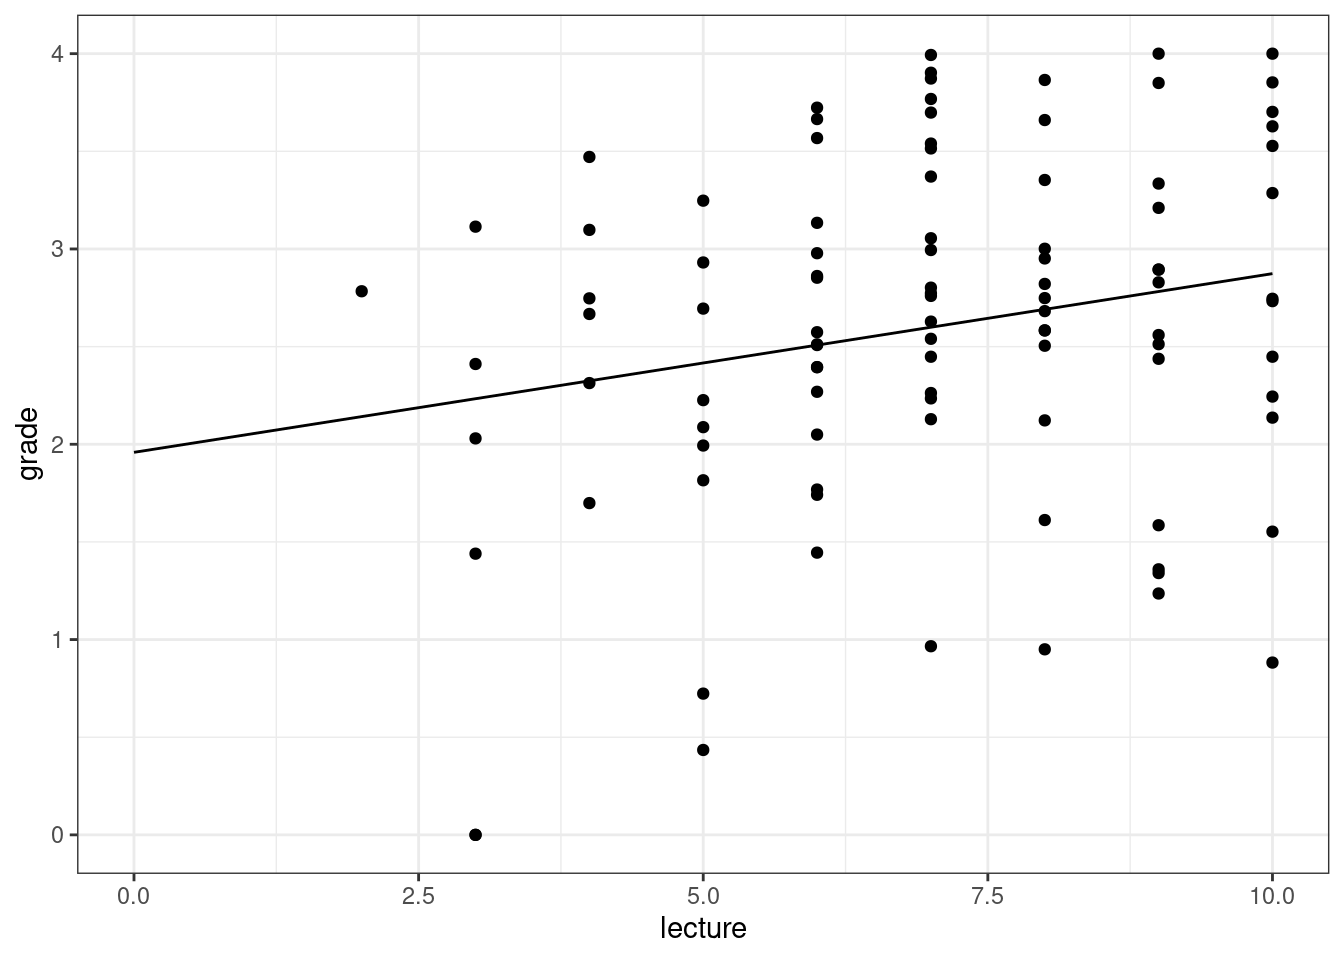
\includegraphics[width=1\linewidth]{03-multiple-regression_files/figure-latex/partial-lecture-plot-1} 

}

\caption{Partial effect of 'lecture' on grade, with nclicks at its mean value.}\label{fig:partial-lecture-plot}
\end{figure}

Partial effect plots only make sense when there are no interactions in the model between the focal predictor and any other predictor.

The reason is that when there are interactions, the partial effect of focal predictor \(X_i\) will differ across the values of the other variables it interacts with.

Now can you visualize the partial effect of \texttt{nclicks} on \texttt{grade}?

See the solution at the bottom of the page.

\hypertarget{standardizing-coefficients}{%
\subsection{Standardizing coefficients}\label{standardizing-coefficients}}

One kind of question that we often use multiple regression to address is, \textbf{Which predictors matter most in predicting Y?}

Now, you can't just read off the \(\hat{\beta}\) values and choose the one with the largest absolute value, because the predictors are all on different scales. To answer this question, you need to \textbf{center} and \textbf{scale} the predictors.

Remember \(z\) scores?

\[
z = \frac{X - \mu_x}{\sigma_x}
\]

A \(z\) score represents the distance of a score \(X\) from the sample mean (\(\mu_x\)) in standard deviation units (\(\sigma_x\)). So a \(z\) score of 1 means that the score is one standard deviation about the mean; a \(z\)-score of -2.5 means 2.5 standard deviations below the mean. \(Z\)-scores give us a way of comparing things that come from different populations by calibrating them to the standard normal distribution (a distribution with a mean of 0 and a standard deviation of 1).

So we re-scale our predictors by converting them to \(z\)-scores. This is easy enough to do.

\begin{Shaded}
\begin{Highlighting}[]
\NormalTok{grades2 <-}\StringTok{ }\NormalTok{grades }\OperatorTok
\StringTok{  }\KeywordTok{mutate}\NormalTok{(}\DataTypeTok{lecture_c =}\NormalTok{ (lecture }\OperatorTok{-}\StringTok{ }\KeywordTok{mean}\NormalTok{(lecture)) }\OperatorTok{/}\StringTok{ }\KeywordTok{sd}\NormalTok{(lecture),}
         \DataTypeTok{nclicks_c =}\NormalTok{ (nclicks }\OperatorTok{-}\StringTok{ }\KeywordTok{mean}\NormalTok{(nclicks)) }\OperatorTok{/}\StringTok{ }\KeywordTok{sd}\NormalTok{(nclicks))}

\NormalTok{grades2}
\end{Highlighting}
\end{Shaded}

\begin{verbatim}
## # A tibble: 100 x 6
##    grade   GPA lecture nclicks lecture_c nclicks_c
##    <dbl> <dbl>   <int>   <int>     <dbl>     <dbl>
##  1  2.40 1.13        6      88  -0.484     -0.666 
##  2  3.67 0.971       6      96  -0.484     -0.150 
##  3  2.85 3.34        6     123  -0.484      1.59  
##  4  1.36 2.76        9      99   0.982      0.0439
##  5  2.31 1.02        4      66  -1.46      -2.09  
##  6  2.58 0.841       8      99   0.493      0.0439
##  7  2.69 4           5      86  -0.972     -0.796 
##  8  3.05 2.29        7     118   0.00488    1.27  
##  9  3.21 3.39        9      98   0.982     -0.0207
## 10  2.24 3.27       10     115   1.47       1.08  
## # ... with 90 more rows
\end{verbatim}

Now let's re-fit the model using the centered and scaled predictors.

\begin{Shaded}
\begin{Highlighting}[]
\NormalTok{my_model_scaled <-}\StringTok{ }\KeywordTok{lm}\NormalTok{(grade }\OperatorTok{~}\StringTok{ }\NormalTok{lecture_c }\OperatorTok{+}\StringTok{ }\NormalTok{nclicks_c, grades2)}

\KeywordTok{summary}\NormalTok{(my_model_scaled)}
\end{Highlighting}
\end{Shaded}

\begin{verbatim}
## 
## Call:
## lm(formula = grade ~ lecture_c + nclicks_c, data = grades2)
## 
## Residuals:
##      Min       1Q   Median       3Q      Max 
## -2.21653 -0.40603  0.02267  0.60720  1.38558 
## 
## Coefficients:
##             Estimate Std. Error t value Pr(>|t|)    
## (Intercept)  2.59839    0.08692  29.895   <2e-16 ***
## lecture_c    0.18734    0.09370   1.999   0.0484 *  
## nclicks_c    0.07823    0.09370   0.835   0.4058    
## ---
## Signif. codes:  0 '***' 0.001 '**' 0.01 '*' 0.05 '.' 0.1 ' ' 1
## 
## Residual standard error: 0.8692 on 97 degrees of freedom
## Multiple R-squared:  0.06543,	Adjusted R-squared:  0.04616 
## F-statistic: 3.395 on 2 and 97 DF,  p-value: 0.03756
\end{verbatim}

This tells us that lecture\_c has a relatively larger influence; for each standard deviation increase in this variable, \texttt{grade} increases by about 0.19.

\hypertarget{model-comparison}{%
\subsection{Model comparison}\label{model-comparison}}

Another common kind of question multiple regression is also used to address is of the form: Does some predictor or set of predictors of interest significantly impact my response variable \textbf{over and above the effects of some control variables}?

For example, we saw above that the model including \texttt{lecture} and \texttt{nclicks} was statistically significant,
\(F(2, 97) = 3.395\),
\(p = 0.038\).

The null hypothesis for a regression model with \(m\) predictors is

\[H_0: \beta_1 = \beta_2 = \ldots = \beta_m = 0;\]

in other words, that all of the coefficients (except the intercept) are zero. If the null hypothesis is true, then the null model

\[Y_i = \beta_0\]

gives just as good of a prediction as the model including all of the predictors and their coefficients. In other words, your best prediction for \(Y\) is just its mean (\(\mu_y\)); the \(X\) variables are irrelevant. We rejected this null hypothesis, which implies that we can do better by including our two predictors, \texttt{lecture} and \texttt{nclicks}.

But you might ask: maybe its the case that better students get better grades, and the relationship between \texttt{lecture}, \texttt{nclicks}, and \texttt{grade} is just mediated by student quality. After all, better students are more likely to go to lecture and download the materials. So we can ask, are attendance and downloads associated with better grades \textbf{above and beyond} student ability, as measured by GPA?

The way we can test this hypothesis is by using \textbf{model comparison}. The logic is as follows. First, estimate a model containing any control predictors but excluding the focal predictors of interest. Second, estimate a model containing the control predictors as well as the focal predictors. Finally, compare the two models, to see if there is any statistically significant gain by including the predictors.

Here is how you do this:

\begin{Shaded}
\begin{Highlighting}[]
\NormalTok{m1 <-}\StringTok{ }\KeywordTok{lm}\NormalTok{(grade }\OperatorTok{~}\StringTok{ }\NormalTok{GPA, grades) }\CommentTok{# control model}
\NormalTok{m2 <-}\StringTok{ }\KeywordTok{lm}\NormalTok{(grade }\OperatorTok{~}\StringTok{ }\NormalTok{GPA }\OperatorTok{+}\StringTok{ }\NormalTok{lecture }\OperatorTok{+}\StringTok{ }\NormalTok{nclicks, grades) }\CommentTok{# bigger model}

\KeywordTok{anova}\NormalTok{(m1, m2)}
\end{Highlighting}
\end{Shaded}

\begin{verbatim}
## Analysis of Variance Table
## 
## Model 1: grade ~ GPA
## Model 2: grade ~ GPA + lecture + nclicks
##   Res.Df    RSS Df Sum of Sq      F Pr(>F)
## 1     98 73.528                           
## 2     96 71.578  2    1.9499 1.3076 0.2752
\end{verbatim}

The null hypothesis is that we are just as good predicting \texttt{grade} from \texttt{GPA} as we are predicting it from \texttt{GPA} plus \texttt{lecture} and \texttt{nclicks}. We will reject the null if adding these two variables leads to a substantial enough reduction in the \textbf{residual sums of squares} (RSS); i.e., if they explain away enough residual variance.

We see that this is not the case:
\(F(2, 96 ) = 1.308\),
\(p = 0.275\). So we don't have evidence that lecture attendance and downloading the online materials is associated with better grades above and beyond student ability, as measured by GPA.

\hypertarget{dealing-with-categorical-predictors}{%
\section{Dealing with categorical predictors}\label{dealing-with-categorical-predictors}}

You can include categorical predictors in a regression model, but first you have to code them as numerical variables. There are a couple of important considerations here.

A \textbf{nominal} variable is a categorical variable for which there is no inherent ordering among the levels of the variable. Pet ownership (cat, dog, ferret) is a nominal variable; cat is not greater than dog and dog is not greater than ferret.

It is common to code nominal variables using numbers. However, you have to be \textbf{very careful} about using numerically-coded nominal variables in your models. If you have a number that is really just a nominal variable, make sure you define it as type \texttt{factor()} before entering it into the model. Otherwise, it will try to treat it as an actual number, and the results of your modeling will be garbage!

It is far too easy to make this mistake, and difficult to catch if authors do not share their data and code. In 2016, \href{https://www.sciencedirect.com/science/article/pii/S0960982216306704}{a paper on religious affiliation and altruism in children that was published in Current Biology had to be retracted for just this kind of mistake}.

\hypertarget{dummy-coding}{%
\subsection{Dummy coding}\label{dummy-coding}}

For a factor with two levels, choose one level as zero and the other as one. The choice is arbitrary, and will affect the sign of the coefficient, but not its standard error or p-value. Here is some code that will do this. Note that if you have a predictor of type character or factor, R will automatically do that for you. We don't want R to do this for reasons that will become apparent in the next lecture, so let's learn how to make our own numeric predictor.

First, we gin up some fake data to use in our analysis.

\begin{Shaded}
\begin{Highlighting}[]
\NormalTok{fake_data <-}\StringTok{ }\KeywordTok{tibble}\NormalTok{(}\DataTypeTok{Y =} \KeywordTok{rnorm}\NormalTok{(}\DecValTok{10}\NormalTok{),}
                    \DataTypeTok{group =} \KeywordTok{rep}\NormalTok{(}\KeywordTok{c}\NormalTok{(}\StringTok{"A"}\NormalTok{, }\StringTok{"B"}\NormalTok{), }\DataTypeTok{each =} \DecValTok{5}\NormalTok{))}

\NormalTok{fake_data}
\end{Highlighting}
\end{Shaded}

\begin{verbatim}
## # A tibble: 10 x 2
##          Y group
##      <dbl> <chr>
##  1  1.32   A    
##  2  0.471  A    
##  3 -1.20   A    
##  4  1.96   A    
##  5 -1.15   A    
##  6 -0.0465 B    
##  7 -0.918  B    
##  8  0.808  B    
##  9  1.38   B    
## 10  0.175  B
\end{verbatim}

Now let's add a new variable, \texttt{group\_d}, which is the dummy coded group variable. We will use the \texttt{dplyr::if\_else()} function to define the new column.

\begin{Shaded}
\begin{Highlighting}[]
\NormalTok{fake_data2 <-}\StringTok{ }\NormalTok{fake_data }\OperatorTok
\StringTok{  }\KeywordTok{mutate}\NormalTok{(}\DataTypeTok{group_d =} \KeywordTok{if_else}\NormalTok{(group }\OperatorTok{==}\StringTok{ "B"}\NormalTok{, }\DecValTok{1}\NormalTok{, }\DecValTok{0}\NormalTok{))}

\NormalTok{fake_data2}
\end{Highlighting}
\end{Shaded}

\begin{verbatim}
## # A tibble: 10 x 3
##          Y group group_d
##      <dbl> <chr>   <dbl>
##  1  1.32   A           0
##  2  0.471  A           0
##  3 -1.20   A           0
##  4  1.96   A           0
##  5 -1.15   A           0
##  6 -0.0465 B           1
##  7 -0.918  B           1
##  8  0.808  B           1
##  9  1.38   B           1
## 10  0.175  B           1
\end{verbatim}

Now we just run it as a regular regression model.

\begin{Shaded}
\begin{Highlighting}[]
\KeywordTok{summary}\NormalTok{(}\KeywordTok{lm}\NormalTok{(Y }\OperatorTok{~}\StringTok{ }\NormalTok{group_d, fake_data2))}
\end{Highlighting}
\end{Shaded}

\begin{verbatim}
## 
## Call:
## lm(formula = Y ~ group_d, data = fake_data2)
## 
## Residuals:
##      Min       1Q   Median       3Q      Max 
## -1.47929 -0.97916  0.04294  0.91025  1.68209 
## 
## Coefficients:
##              Estimate Std. Error t value Pr(>|t|)
## (Intercept)  0.280742   0.529374   0.530    0.610
## group_d     -0.001728   0.748647  -0.002    0.998
## 
## Residual standard error: 1.184 on 8 degrees of freedom
## Multiple R-squared:  6.663e-07,	Adjusted R-squared:  -0.125 
## F-statistic: 5.33e-06 on 1 and 8 DF,  p-value: 0.9982
\end{verbatim}

Note that if we reverse the coding we get the same result, just the sign is different.

\begin{Shaded}
\begin{Highlighting}[]
\NormalTok{fake_data3 <-}\StringTok{ }\NormalTok{fake_data }\OperatorTok
\StringTok{  }\KeywordTok{mutate}\NormalTok{(}\DataTypeTok{group_d =} \KeywordTok{if_else}\NormalTok{(group }\OperatorTok{==}\StringTok{ "A"}\NormalTok{, }\DecValTok{1}\NormalTok{, }\DecValTok{0}\NormalTok{))}

\KeywordTok{summary}\NormalTok{(}\KeywordTok{lm}\NormalTok{(Y }\OperatorTok{~}\StringTok{ }\NormalTok{group_d, fake_data3))}
\end{Highlighting}
\end{Shaded}

\begin{verbatim}
## 
## Call:
## lm(formula = Y ~ group_d, data = fake_data3)
## 
## Residuals:
##      Min       1Q   Median       3Q      Max 
## -1.47929 -0.97916  0.04294  0.91025  1.68209 
## 
## Coefficients:
##             Estimate Std. Error t value Pr(>|t|)
## (Intercept) 0.279013   0.529374   0.527    0.612
## group_d     0.001728   0.748647   0.002    0.998
## 
## Residual standard error: 1.184 on 8 degrees of freedom
## Multiple R-squared:  6.663e-07,	Adjusted R-squared:  -0.125 
## F-statistic: 5.33e-06 on 1 and 8 DF,  p-value: 0.9982
\end{verbatim}

The interpretation of the intercept is the estimated mean for the group coded as zero. You can see by plugging in zero for X in the prediction formula below. Thus, \(\beta_1\) can be interpreted as the difference between the mean for the baseline group and the group coded as 1.

\[\hat{Y_i} = \hat{\beta}_0 + \hat{\beta}_1 X_i \]

\hypertarget{dummy-coding-when-k-2}{%
\subsection{\texorpdfstring{Dummy coding when \(k > 2\)}{Dummy coding when k \textgreater{} 2}}\label{dummy-coding-when-k-2}}

When the predictor variable is a factor with \(k\) levels where \(k>2\), we need \(k-1\) predictors to code that variable. So if the factor has 4 levels, we'll need to define three predictors. Here is code to do that. Try it out and see if you can figure out how it works.

\begin{Shaded}
\begin{Highlighting}[]
\NormalTok{mydata <-}\StringTok{ }\KeywordTok{tibble}\NormalTok{(}\DataTypeTok{season =} \KeywordTok{rep}\NormalTok{(}\KeywordTok{c}\NormalTok{(}\StringTok{"winter"}\NormalTok{, }\StringTok{"spring"}\NormalTok{, }\StringTok{"summer"}\NormalTok{, }\StringTok{"fall"}\NormalTok{), }\DataTypeTok{each =} \DecValTok{5}\NormalTok{),}
                 \DataTypeTok{bodyweight_kg =} \KeywordTok{c}\NormalTok{(}\KeywordTok{rnorm}\NormalTok{(}\DecValTok{5}\NormalTok{, }\DecValTok{105}\NormalTok{, }\DecValTok{3}\NormalTok{),}
                                   \KeywordTok{rnorm}\NormalTok{(}\DecValTok{5}\NormalTok{, }\DecValTok{103}\NormalTok{, }\DecValTok{3}\NormalTok{),}
                                   \KeywordTok{rnorm}\NormalTok{(}\DecValTok{5}\NormalTok{, }\DecValTok{101}\NormalTok{, }\DecValTok{3}\NormalTok{),}
                                   \KeywordTok{rnorm}\NormalTok{(}\DecValTok{5}\NormalTok{, }\FloatTok{102.5}\NormalTok{, }\DecValTok{3}\NormalTok{)))}

\NormalTok{mydata}
\end{Highlighting}
\end{Shaded}

\begin{verbatim}
## # A tibble: 20 x 2
##    season bodyweight_kg
##    <chr>          <dbl>
##  1 winter         107. 
##  2 winter         102. 
##  3 winter         105. 
##  4 winter         105. 
##  5 winter         103. 
##  6 spring         104. 
##  7 spring         101. 
##  8 spring         105. 
##  9 spring         108. 
## 10 spring         102. 
## 11 summer         101. 
## 12 summer         100. 
## 13 summer          98.8
## 14 summer         101. 
## 15 summer         104. 
## 16 fall            99.5
## 17 fall           102. 
## 18 fall           102. 
## 19 fall           101. 
## 20 fall            99.0
\end{verbatim}

Now let's add three predictors to code the variable \texttt{season}.

\begin{Shaded}
\begin{Highlighting}[]
\CommentTok{## baseline value is 'winter'}
\NormalTok{mydata2 <-}\StringTok{ }\NormalTok{mydata }\OperatorTok
\StringTok{  }\KeywordTok{mutate}\NormalTok{(}\DataTypeTok{V1 =} \KeywordTok{if_else}\NormalTok{(season }\OperatorTok{==}\StringTok{ "spring"}\NormalTok{, }\DecValTok{1}\NormalTok{, }\DecValTok{0}\NormalTok{),}
         \DataTypeTok{V2 =} \KeywordTok{if_else}\NormalTok{(season }\OperatorTok{==}\StringTok{ "summer"}\NormalTok{, }\DecValTok{1}\NormalTok{, }\DecValTok{0}\NormalTok{),}
         \DataTypeTok{V3 =} \KeywordTok{if_else}\NormalTok{(season }\OperatorTok{==}\StringTok{ "fall"}\NormalTok{, }\DecValTok{1}\NormalTok{, }\DecValTok{0}\NormalTok{))}

\NormalTok{mydata2}
\end{Highlighting}
\end{Shaded}

\begin{verbatim}
## # A tibble: 20 x 5
##    season bodyweight_kg    V1    V2    V3
##    <chr>          <dbl> <dbl> <dbl> <dbl>
##  1 winter         107.      0     0     0
##  2 winter         102.      0     0     0
##  3 winter         105.      0     0     0
##  4 winter         105.      0     0     0
##  5 winter         103.      0     0     0
##  6 spring         104.      1     0     0
##  7 spring         101.      1     0     0
##  8 spring         105.      1     0     0
##  9 spring         108.      1     0     0
## 10 spring         102.      1     0     0
## 11 summer         101.      0     1     0
## 12 summer         100.      0     1     0
## 13 summer          98.8     0     1     0
## 14 summer         101.      0     1     0
## 15 summer         104.      0     1     0
## 16 fall            99.5     0     0     1
## 17 fall           102.      0     0     1
## 18 fall           102.      0     0     1
## 19 fall           101.      0     0     1
## 20 fall            99.0     0     0     1
\end{verbatim}

\hypertarget{equivalence-between-multiple-regression-and-one-way-anova}{%
\section{Equivalence between multiple regression and one-way ANOVA}\label{equivalence-between-multiple-regression-and-one-way-anova}}

If we wanted to see whether our bodyweight varies over season, we could do a one way ANOVA on \texttt{mydata2} like so.

\begin{Shaded}
\begin{Highlighting}[]
\CommentTok{## make season into a factor with baseline level 'winter'}
\NormalTok{mydata3 <-}\StringTok{ }\NormalTok{mydata2 }\OperatorTok
\StringTok{  }\KeywordTok{mutate}\NormalTok{(}\DataTypeTok{season =} \KeywordTok{factor}\NormalTok{(season, }\DataTypeTok{levels =} \KeywordTok{c}\NormalTok{(}\StringTok{"winter"}\NormalTok{, }\StringTok{"spring"}\NormalTok{, }\StringTok{"summer"}\NormalTok{, }\StringTok{"fall"}\NormalTok{)))}

\NormalTok{my_anova <-}\StringTok{ }\KeywordTok{aov}\NormalTok{(bodyweight_kg }\OperatorTok{~}\StringTok{ }\NormalTok{season, mydata3)}
\KeywordTok{summary}\NormalTok{(my_anova)}
\end{Highlighting}
\end{Shaded}

\begin{verbatim}
##             Df Sum Sq Mean Sq F value Pr(>F)  
## season       3  59.14  19.714   5.155  0.011 *
## Residuals   16  61.19   3.824                 
## ---
## Signif. codes:  0 '***' 0.001 '**' 0.01 '*' 0.05 '.' 0.1 ' ' 1
\end{verbatim}

OK, now can we replicate that result using the regression model below?

\[Y_i = \beta_0 + \beta_1 X_{1i} + \beta_2 X_{2i} + \beta_3 X_{3i} + e_i\]

\begin{Shaded}
\begin{Highlighting}[]
\KeywordTok{summary}\NormalTok{(}\KeywordTok{lm}\NormalTok{(bodyweight_kg }\OperatorTok{~}\StringTok{ }\NormalTok{V1 }\OperatorTok{+}\StringTok{ }\NormalTok{V2 }\OperatorTok{+}\StringTok{ }\NormalTok{V3, mydata3))}
\end{Highlighting}
\end{Shaded}

\begin{verbatim}
## 
## Call:
## lm(formula = bodyweight_kg ~ V1 + V2 + V3, data = mydata3)
## 
## Residuals:
##     Min      1Q  Median      3Q     Max 
## -2.6048 -1.4881  0.0902  0.9071  3.5717 
## 
## Coefficients:
##             Estimate Std. Error t value Pr(>|t|)    
## (Intercept) 104.5803     0.8746 119.582  < 2e-16 ***
## V1           -0.5034     1.2368  -0.407  0.68936    
## V2           -3.4053     1.2368  -2.753  0.01414 *  
## V3           -3.9033     1.2368  -3.156  0.00612 ** 
## ---
## Signif. codes:  0 '***' 0.001 '**' 0.01 '*' 0.05 '.' 0.1 ' ' 1
## 
## Residual standard error: 1.956 on 16 degrees of freedom
## Multiple R-squared:  0.4915,	Adjusted R-squared:  0.3962 
## F-statistic: 5.155 on 3 and 16 DF,  p-value: 0.01104
\end{verbatim}

Note that the \(F\) values and \(p\) values are identical for the two methods!

\hypertarget{solution-to-partial-effect-plot}{%
\section{Solution to partial effect plot}\label{solution-to-partial-effect-plot}}

First create a tibble with new predictors. We might also want to know the range of values that \texttt{nclicks} varies over.

\begin{Shaded}
\begin{Highlighting}[]
\NormalTok{lecture_mean <-}\StringTok{ }\NormalTok{grades }\OperatorTok\StringTok{ }\KeywordTok{pull}\NormalTok{(lecture) }\OperatorTok\StringTok{ }\KeywordTok{mean}\NormalTok{()}
\NormalTok{min_nclicks <-}\StringTok{ }\NormalTok{grades }\OperatorTok\StringTok{ }\KeywordTok{pull}\NormalTok{(nclicks) }\OperatorTok\StringTok{ }\KeywordTok{min}\NormalTok{()}
\NormalTok{max_nclicks <-}\StringTok{ }\NormalTok{grades }\OperatorTok\StringTok{ }\KeywordTok{pull}\NormalTok{(nclicks) }\OperatorTok\StringTok{ }\KeywordTok{max}\NormalTok{()}

\CommentTok{## new data for prediction}
\NormalTok{new_nclicks <-}\StringTok{ }\KeywordTok{tibble}\NormalTok{(}\DataTypeTok{lecture =}\NormalTok{ lecture_mean,}
                      \DataTypeTok{nclicks =}\NormalTok{ min_nclicks}\OperatorTok{:}\NormalTok{max_nclicks)}

\CommentTok{## add the predicted value to new_lecture}
\NormalTok{new_nclicks2 <-}\StringTok{ }\NormalTok{new_nclicks }\OperatorTok
\StringTok{  }\KeywordTok{mutate}\NormalTok{(}\DataTypeTok{grade =} \KeywordTok{predict}\NormalTok{(my_model, new_nclicks))}

\NormalTok{new_nclicks2}
\end{Highlighting}
\end{Shaded}

\begin{verbatim}
## # A tibble: 76 x 3
##    lecture nclicks grade
##      <dbl>   <int> <dbl>
##  1    6.99      54  2.37
##  2    6.99      55  2.38
##  3    6.99      56  2.38
##  4    6.99      57  2.39
##  5    6.99      58  2.39
##  6    6.99      59  2.40
##  7    6.99      60  2.40
##  8    6.99      61  2.41
##  9    6.99      62  2.41
## 10    6.99      63  2.42
## # ... with 66 more rows
\end{verbatim}

Now plot.

\begin{Shaded}
\begin{Highlighting}[]
\KeywordTok{ggplot}\NormalTok{(grades, }\KeywordTok{aes}\NormalTok{(nclicks, grade)) }\OperatorTok{+}
\StringTok{  }\KeywordTok{geom_point}\NormalTok{() }\OperatorTok{+}
\StringTok{  }\KeywordTok{geom_line}\NormalTok{(}\DataTypeTok{data =}\NormalTok{ new_nclicks2)}
\end{Highlighting}
\end{Shaded}

\begin{figure}

{\centering 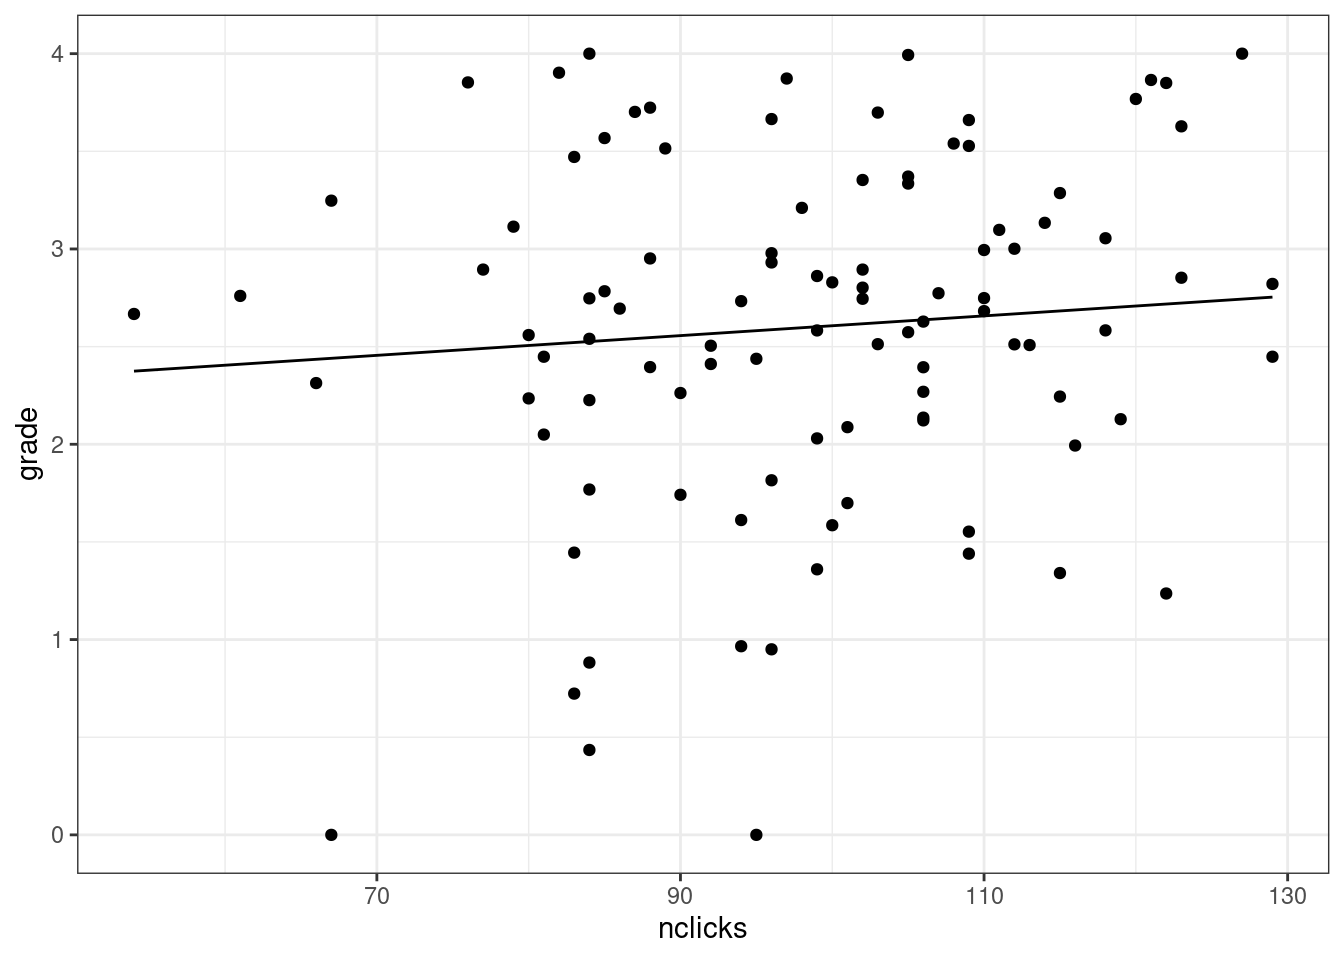
\includegraphics[width=1\linewidth]{03-multiple-regression_files/figure-latex/partial-nclicks-1} 

}

\caption{Partial effect plot of nclicks on grade.}\label{fig:partial-nclicks}
\end{figure}

\hypertarget{interactions}{%
\chapter{Interactions}\label{interactions}}

\hypertarget{learning-objectives}{%
\section{Learning objectives}\label{learning-objectives}}

\begin{itemize}
\tightlist
\item
  model and interpret continuous-by-categorical interactions
\item
  model and interpret categorical-by-categorical interactions in factorial designs
\item
  estimate and test effects in factorial designs using ANOVA or regression
\end{itemize}

\hypertarget{interactions-1}{%
\section{Interactions}\label{interactions-1}}

Up to now, we've been focusing on estimating and interpreting the effect of a variable or linear combination of predictor variables on a response variable. However, there are often situations where the effect of one predictor on the response depends on the value of another predictor variable. We can actually estimate and interpret this dependency as well, by including an \textbf{interaction} term in our model.

\hypertarget{cont-by-cat}{%
\section{Continuous-by-Categorical Interactions}\label{cont-by-cat}}

One common example of this is when you are interested in whether a linear relationship between a continous predictor and a continuous response is different for two groups.

Let's consider a simple fictional example. Say you are interested in the effects of sonic distraction on cognitive performance. Each participant in your study is randomly assigned to receive a particular amount of sonic distraction while they perform a simple reaction time task (respond as quickly as possible to a flashing light). You have a technique that allows you to automatically generate different levels of background noise (e.g., frequency and amplitude of city sounds, such as sirens, jackhammers, people yelling, glass breaking, etc.). Each participant performs the task for a randomly chosen level of distraction (0 to 100). Your hypothesis is that urban living makes people's task performance more immune to sonic distraction. You want to compare the relationship between distraction and performance for city dwellers to the relationship for people from quieter rural environments.

You have three variables:

\begin{itemize}
\tightlist
\item
  A continuous response variable, \texttt{mean\_RT}, with higher levels reflecting slower RTs;
\item
  A continuous predictor variable, level of sonic distraction (\texttt{dist\_level}), with higher levels indicating more distraction;
\item
  A factor with two levels, \texttt{group} (urban vs.~rural).
\end{itemize}

Let's start by simulating some data for the urban group. Let's assume that with zero distraction (silence), the average RT is about 450 milliseconds, and that with each unit increase on the distraction scale, RT increases about 2 ms. This gives us the following linear model:

\[Y_i = 450 + 2 X_i + e_i\]

where \(X_i\) is the amount of sonic distraction.

Let's simulate data for 100 participants as below with \(\sigma = 80\), setting the seed before we begin.

\begin{Shaded}
\begin{Highlighting}[]
\KeywordTok{library}\NormalTok{(}\StringTok{"tidyverse"}\NormalTok{)}
\KeywordTok{set.seed}\NormalTok{(}\DecValTok{1031}\NormalTok{)}

\NormalTok{n_subj <-}\StringTok{ }\NormalTok{100L  }\CommentTok{# simulate data for 100 subjects}
\NormalTok{b0_urban <-}\StringTok{ }\DecValTok{450} \CommentTok{# y-intercept}
\NormalTok{b1_urban <-}\StringTok{ }\DecValTok{2}   \CommentTok{# slope}

\CommentTok{# decomposition table}
\NormalTok{urban <-}\StringTok{ }\KeywordTok{tibble}\NormalTok{(}
  \DataTypeTok{subj_id =} \DecValTok{1}\OperatorTok{:}\NormalTok{n_subj,}
  \DataTypeTok{group =} \StringTok{"urban"}\NormalTok{,}
  \DataTypeTok{b0 =} \DecValTok{450}\NormalTok{,}
  \DataTypeTok{b1 =} \DecValTok{2}\NormalTok{,}
  \DataTypeTok{dist_level =} \KeywordTok{sample}\NormalTok{(}\DecValTok{0}\OperatorTok{:}\NormalTok{n_subj, n_subj, }\DataTypeTok{replace =} \OtherTok{TRUE}\NormalTok{),}
  \DataTypeTok{err =} \KeywordTok{rnorm}\NormalTok{(n_subj, }\DataTypeTok{mean =} \DecValTok{0}\NormalTok{, }\DataTypeTok{sd =} \DecValTok{80}\NormalTok{),}
  \DataTypeTok{simple_rt =}\NormalTok{ b0 }\OperatorTok{+}\StringTok{ }\NormalTok{b1 }\OperatorTok{*}\StringTok{ }\NormalTok{dist_level }\OperatorTok{+}\StringTok{ }\NormalTok{err)}

\NormalTok{urban}
\end{Highlighting}
\end{Shaded}

\begin{verbatim}
## # A tibble: 100 x 7
##    subj_id group    b0    b1 dist_level     err simple_rt
##      <int> <chr> <dbl> <dbl>      <int>   <dbl>     <dbl>
##  1       1 urban   450     2         59  -36.1       532.
##  2       2 urban   450     2         45  128.        668.
##  3       3 urban   450     2         55   23.5       584.
##  4       4 urban   450     2          8    1.04      467.
##  5       5 urban   450     2         47   48.7       593.
##  6       6 urban   450     2         96   88.2       730.
##  7       7 urban   450     2         62  110.        684.
##  8       8 urban   450     2          8  -91.6       374.
##  9       9 urban   450     2         15 -109.        371.
## 10      10 urban   450     2         70   20.7       611.
## # ... with 90 more rows
\end{verbatim}

Let's plot the data we created, along with the line of best fit.

\begin{Shaded}
\begin{Highlighting}[]
\KeywordTok{ggplot}\NormalTok{(urban, }\KeywordTok{aes}\NormalTok{(dist_level, simple_rt)) }\OperatorTok{+}\StringTok{ }
\StringTok{  }\KeywordTok{geom_point}\NormalTok{(}\DataTypeTok{alpha =} \FloatTok{.2}\NormalTok{) }\OperatorTok{+}
\StringTok{  }\KeywordTok{geom_smooth}\NormalTok{(}\DataTypeTok{method =} \StringTok{"lm"}\NormalTok{, }\DataTypeTok{se =} \OtherTok{FALSE}\NormalTok{)}
\end{Highlighting}
\end{Shaded}

\begin{verbatim}
## `geom_smooth()` using formula 'y ~ x'
\end{verbatim}

\begin{figure}

{\centering 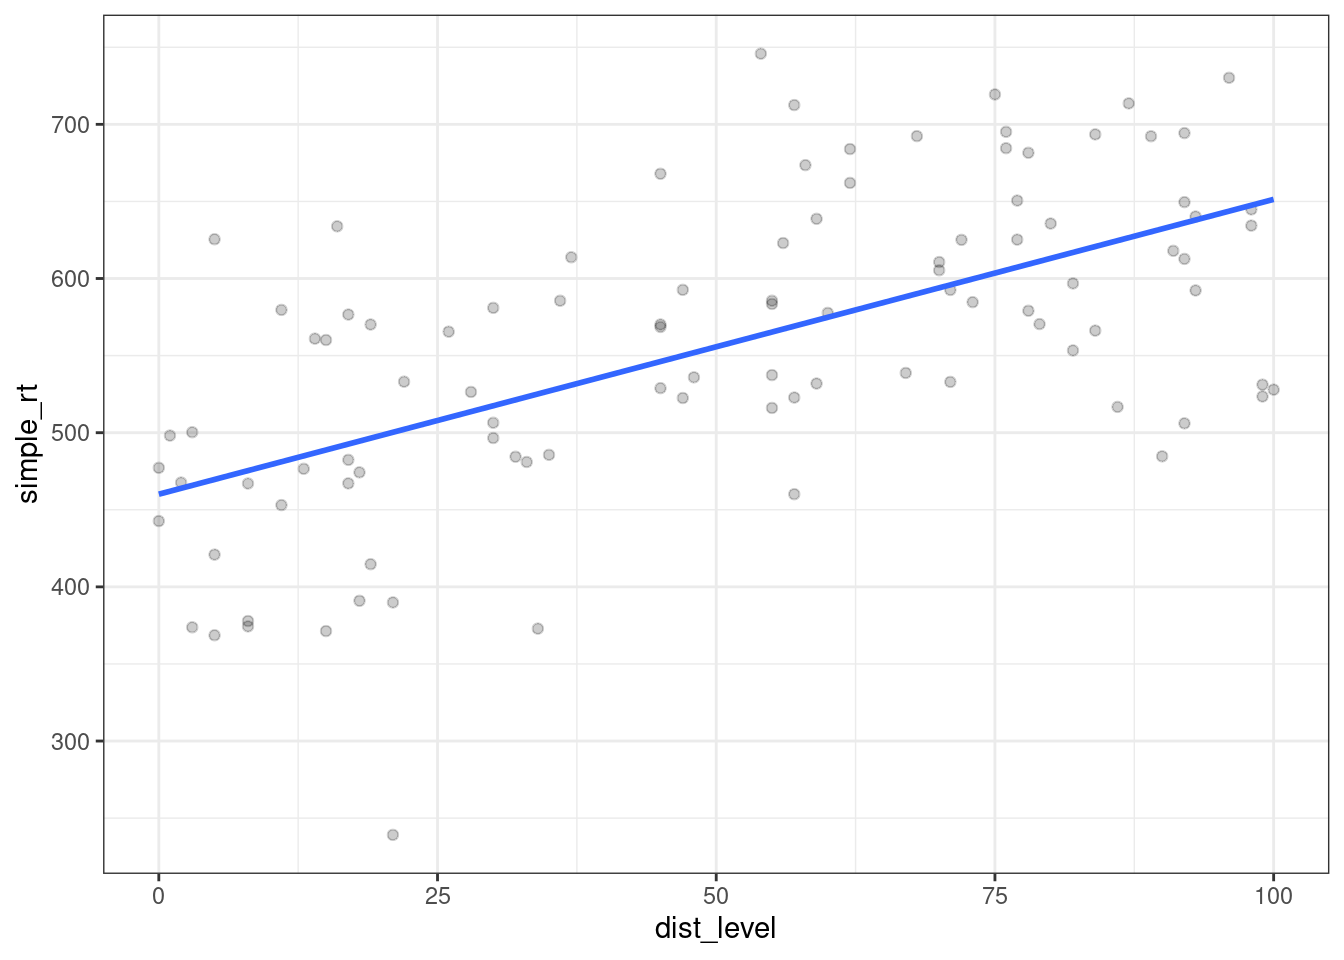
\includegraphics[width=1\linewidth]{04-interactions_files/figure-latex/plot-urban-1} 

}

\caption{*Effect of sonic distraction on simple RT, urban group.*}\label{fig:plot-urban}
\end{figure}

Now let's simulate data for the urban group. We assume that these participants should perhaps have a little higher intercept, maybe because they are less familiar with technology. Most importantly, we assume that they would have a steeper slope because they are more affected by the noise. Something like:

\[Y_i = 500 + 3 X_i + e_i\]

\begin{Shaded}
\begin{Highlighting}[]
\NormalTok{b0_rural <-}\StringTok{ }\DecValTok{500}
\NormalTok{b1_rural <-}\StringTok{ }\DecValTok{3}

\NormalTok{rural <-}\StringTok{ }\KeywordTok{tibble}\NormalTok{(}
  \DataTypeTok{subj_id =} \DecValTok{1}\OperatorTok{:}\NormalTok{n_subj }\OperatorTok{+}\StringTok{ }\NormalTok{n_subj,}
  \DataTypeTok{group =} \StringTok{"rural"}\NormalTok{,}
  \DataTypeTok{b0 =}\NormalTok{ b0_rural,}
  \DataTypeTok{b1 =}\NormalTok{ b1_rural,}
  \DataTypeTok{dist_level =} \KeywordTok{sample}\NormalTok{(}\DecValTok{0}\OperatorTok{:}\NormalTok{n_subj, n_subj, }\DataTypeTok{replace =} \OtherTok{TRUE}\NormalTok{),}
  \DataTypeTok{err =} \KeywordTok{rnorm}\NormalTok{(n_subj, }\DataTypeTok{mean =} \DecValTok{0}\NormalTok{, }\DataTypeTok{sd =} \DecValTok{80}\NormalTok{),}
  \DataTypeTok{simple_rt =}\NormalTok{ b0 }\OperatorTok{+}\StringTok{ }\NormalTok{b1 }\OperatorTok{*}\StringTok{ }\NormalTok{dist_level }\OperatorTok{+}\StringTok{ }\NormalTok{err)}
\end{Highlighting}
\end{Shaded}

Now let's plot the data from the two groups side by side.

\begin{Shaded}
\begin{Highlighting}[]
\NormalTok{all_data <-}\StringTok{ }\KeywordTok{bind_rows}\NormalTok{(urban, rural)}

\KeywordTok{ggplot}\NormalTok{(all_data }\OperatorTok\StringTok{ }\KeywordTok{mutate}\NormalTok{(}\DataTypeTok{group =} \KeywordTok{fct_relevel}\NormalTok{(group, }\StringTok{"urban"}\NormalTok{)), }
       \KeywordTok{aes}\NormalTok{(dist_level, simple_rt, }\DataTypeTok{colour =}\NormalTok{ group)) }\OperatorTok{+}
\StringTok{  }\KeywordTok{geom_point}\NormalTok{() }\OperatorTok{+}
\StringTok{  }\KeywordTok{geom_smooth}\NormalTok{(}\DataTypeTok{method =} \StringTok{"lm"}\NormalTok{, }\DataTypeTok{se =} \OtherTok{FALSE}\NormalTok{) }\OperatorTok{+}
\StringTok{  }\KeywordTok{facet_wrap}\NormalTok{(}\OperatorTok{~}\StringTok{ }\NormalTok{group) }\OperatorTok{+}\StringTok{ }
\StringTok{  }\KeywordTok{theme}\NormalTok{(}\DataTypeTok{legend.position =} \StringTok{"none"}\NormalTok{)}
\end{Highlighting}
\end{Shaded}

\begin{verbatim}
## `geom_smooth()` using formula 'y ~ x'
\end{verbatim}

\begin{figure}

{\centering 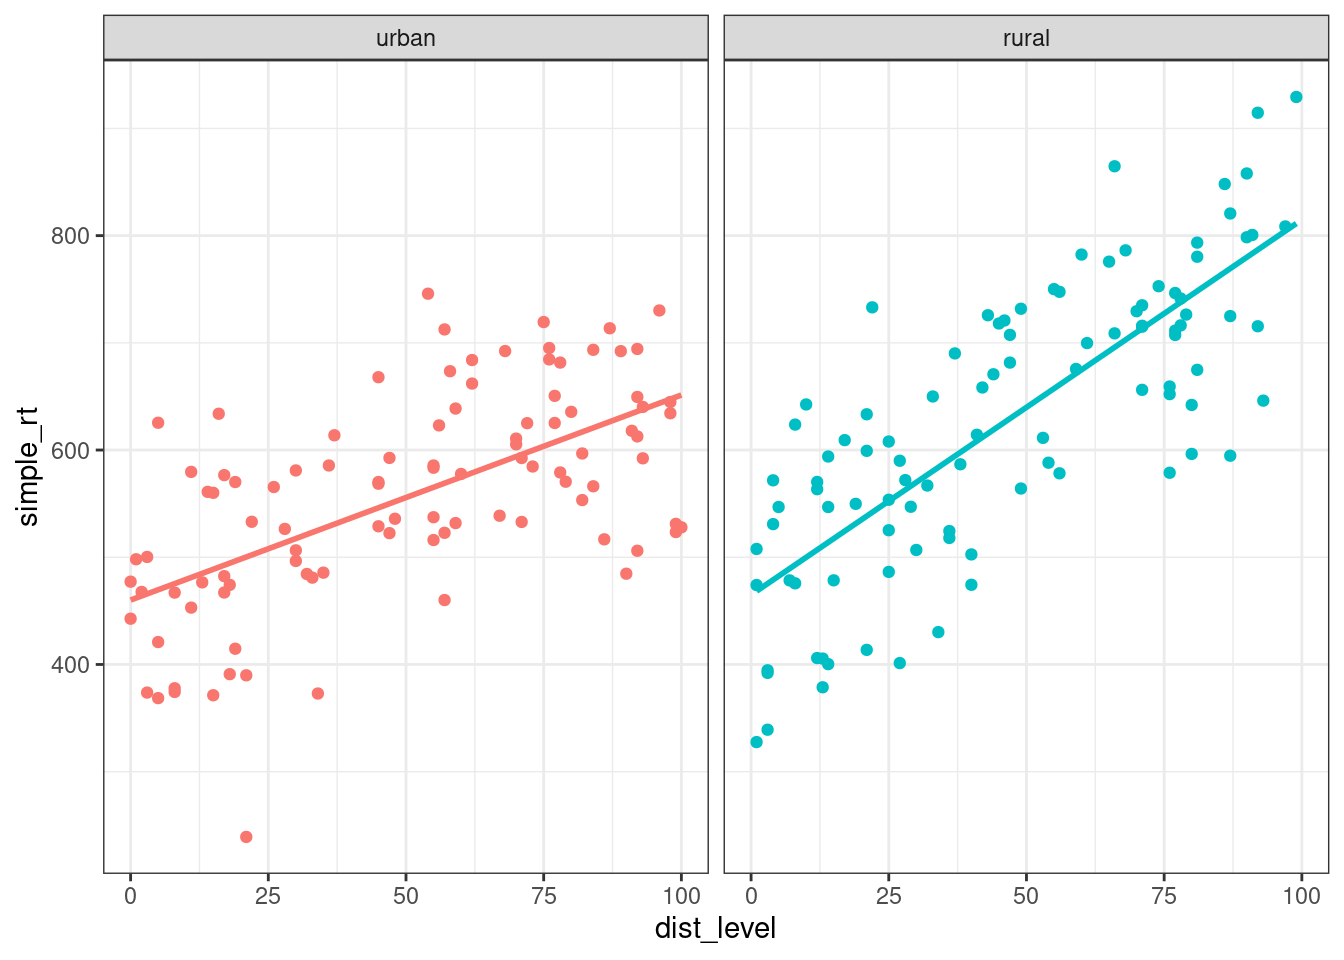
\includegraphics[width=1\linewidth]{04-interactions_files/figure-latex/combined-plot-1} 

}

\caption{*Effect of sonic distraction on simple RT for urban and rural participants.*}\label{fig:combined-plot}
\end{figure}

Here we see very clearly the difference in slope that we built into our data. How do we test whether the two slopes are significantly different? To do this, we can't have two separate regressions. We need to bring the two regression lines into the same model. How do we do this?

Note that we can represent one of the regression lines in terms of `offset' values from the other. We (arbitrarily) choose one group as our `baseline' group, and represent the y-intercept and slope of the other group as offsets from this baseline. So if we choose the urban group as our baseline, we can express the y-intercept and slope for the rural group in terms of two offsets, \(\beta_2\) and \(\beta_3\), for the y-intercept and slope, respectively.

\begin{itemize}
\tightlist
\item
  y-intercept: \(\beta_{0\_rural} = \beta_{0\_urban} + \beta_2\)
\item
  slope: \(\beta_{1\_rural} = \beta_{1\_urban} + \beta_3\)
\end{itemize}

Our urban group had parameters \(\beta_{0\_urban} = 450\) (\texttt{b0\_urban\ \textless{}-\ 450}) and \(\beta_{1\_urban} = 2\) (\texttt{b1\_urban\ \textless{}-\ 2}), whereas the rural broup had \(\beta_{0\_rural} = 500\) (\texttt{b0\_rural\ \textless{}-\ 500}) and \(\beta_{1\_rural} = 3\) (\texttt{b1\_rural\ \textless{}-\ 3}). It directly follows that \(\beta_2 = 50\) and \(\beta_3 = 1\) for our simulated example.

So our two regression models are now:

\[Y_{i\_urban} = \beta_{0\_urban} + \beta_{1\_urban} X_i + e_i\]

and

\[Y_{i\_rural} = (\beta_{0\_urban} + \beta_2) + (\beta_{1\_urban} + \beta_3) X_i + e_i.\]

OK, we feel like we're closer to getting these into a single regression model. Here's the final trick. We define an additional dummy predictor variable that takes on the value 0 for the urban group (which we chose as our `baseline' group) and 1 for the other group. Our final model takes the following form.

\textbf{Regression model with a continuous-by-categorical interaction.}

\[Y_{i} = \beta_0 + \beta_1 X_{1i} + \beta_2 X_{2i} + \beta_3 X_{1i} X_{2i} + e_{i}\]

where

\begin{itemize}
\tightlist
\item
  \(X_{1i}\) is the continous predictor, and
\item
  \(X_{2i}\) is a dummy-coded variable taking on 0 for the baseline, 1 for the alternative group.
\end{itemize}

Interpretation of parameters:

\begin{itemize}
\tightlist
\item
  \(\beta_0\): y-intercept for the baseline group;
\item
  \(\beta_1\): slope for the baseline group;
\item
  \(\beta_2\): offset to y-intercept for the alternative group;
\item
  \(\beta_3\): offset to slope for the alternative group.
\end{itemize}

Estimation in R:

\texttt{lm(Y\ \textasciitilde{}\ X1\ +\ X2\ +\ X1:X2,\ data)} or, as a shortcut:

\texttt{lm(Y\ \textasciitilde{}\ X1\ *\ X2)} where \texttt{*} means ``all possible main effects and interactions of X1 and X2''

The term associated with \(\beta_3\) is an \textbf{interaction term}, where the predictor is the product of predictor values. Let's now show that the above GLM gives us the two regression lines that we want. Plugging in 0 for \(X_{2i}\) and reducing gives us

\[Y_{i} = \beta_0 + \beta_1 X_{1i} + \beta_2 0 + \beta_3 X_{1i} 0 + e_i\]

which is just

\[Y_{i} = \beta_0 + \beta_1 X_{1i} + e_i,\]

the regression equation for our baseline (urban) group. Compare this to \(Y_{i\_urban}\) above.

Plugging in 1 for \(X_{2i}\) should give us the equation for our rural group. We get

\[Y_{i} = \beta_0 + \beta_1 X_{1i} + \beta_2 1 + \beta_3 X_{1i} 1 + e_i\]

which, after reducing and applying a little algebra, can also be expressed as

\[Y_{i} = \beta_0 + \beta_2 + (\beta_1 + \beta_3) X_{1i} + e_i.\]

Compare this to \(Y_{i\_rural}\) above. The dummy-coding trick works!

Now let's see how to estimate the regression in R. Let's say we wanted to test the hypothesis that the slopes for the two lines are different. Note that this just amounts to testing the null hypothesis that \(\beta_3 = 0\), because \(\beta_3\) is our slope offset.

We have already created the dataset \texttt{all\_data} combining the simulated data for our two groups. The way we express our model using R formula syntax is \texttt{Y\ \textasciitilde{}\ X1\ +\ X2\ +\ X1:X2} where \texttt{X1:X2} tells R to create a predictor that is the product of predictors X1 and X2. There is a shortcut \texttt{Y\ \textasciitilde{}\ X1\ *\ X2} which tells R to calculate all possible main effects and interactions. First we'll add a dummy predictor to our model, storing the result in \texttt{all\_data2}.

\begin{Shaded}
\begin{Highlighting}[]
\NormalTok{all_data2 <-}\StringTok{ }\NormalTok{all_data }\OperatorTok
\StringTok{  }\KeywordTok{mutate}\NormalTok{(}\DataTypeTok{grp =} \KeywordTok{if_else}\NormalTok{(group }\OperatorTok{==}\StringTok{ "rural"}\NormalTok{, }\DecValTok{1}\NormalTok{, }\DecValTok{0}\NormalTok{))}
\end{Highlighting}
\end{Shaded}

\begin{Shaded}
\begin{Highlighting}[]
\NormalTok{sonic_mod <-}\StringTok{ }\KeywordTok{lm}\NormalTok{(simple_rt }\OperatorTok{~}\StringTok{ }\NormalTok{dist_level }\OperatorTok{+}\StringTok{ }\NormalTok{grp }\OperatorTok{+}\StringTok{ }\NormalTok{dist_level}\OperatorTok{:}\NormalTok{grp, all_data2)}

\KeywordTok{summary}\NormalTok{(sonic_mod)}
\end{Highlighting}
\end{Shaded}

\begin{verbatim}
## 
## Call:
## lm(formula = simple_rt ~ dist_level + grp + dist_level:grp, data = all_data2)
## 
## Residuals:
##      Min       1Q   Median       3Q      Max 
## -261.130  -50.749    3.617   62.304  191.211 
## 
## Coefficients:
##                Estimate Std. Error t value Pr(>|t|)    
## (Intercept)    460.1098    15.5053  29.674  < 2e-16 ***
## dist_level       1.9123     0.2620   7.299 7.07e-12 ***
## grp              4.8250    21.7184   0.222    0.824    
## dist_level:grp   1.5865     0.3809   4.166 4.65e-05 ***
## ---
## Signif. codes:  0 '***' 0.001 '**' 0.01 '*' 0.05 '.' 0.1 ' ' 1
## 
## Residual standard error: 81.14 on 196 degrees of freedom
## Multiple R-squared:  0.5625,	Adjusted R-squared:  0.5558 
## F-statistic: 83.99 on 3 and 196 DF,  p-value: < 2.2e-16
\end{verbatim}

Can you identify the values of the regression coefficients in the output?

\hypertarget{categorical-by-categorical-interactions}{%
\section{Categorical-by-Categorical Interactions}\label{categorical-by-categorical-interactions}}

\textbf{Factorial designs} are very common in psychology, and are most often analyzed using ANOVA-based techniques, which can obscure that they are also just models.

A factorial design is one in which the predictors (IVs) are all categorical: each is a \textbf{factor} having a fixed number of \textbf{levels}. In a full-factorial design, the factors are fully crossed with each other such that each possible combination of factors is represented. We call each unique combination a \textbf{cell} of the design. You will often hear designs referred to as ``a two-by-two design'' (2x2), which means that there are two factors, each of which has three levels. A ``three-by-three'' (3x3) design is one where there are two factors, each with three levels; a ``two-by-two-by-two'' 2x2x2 design is one in which there are three factors, each with two levels; and so on.

Typically, factorial designs are given a tabular representation, showing all the combinations of factor levels. Below is a tabular representation of a 2x2 design.

\begin{table}[H]
\centering
\begin{tabular}{l|l|l}
\hline
  & \$B\_1\$ & \$B\_2\$\\
\hline
\$A\_1\$ & \$AB\_\{11\}\$ & \$AB\_\{12\}\$\\
\hline
\$A\_2\$ & \$AB\_\{21\}\$ & \$AB\_\{22\}\$\\
\hline
\end{tabular}
\end{table}

A 3x2 design might be shown as follows.

\begin{table}[H]
\centering
\begin{tabular}{l|l|l}
\hline
  & \$B\_1\$ & \$B\_2\$\\
\hline
\$A\_1\$ & \$AB\_\{11\}\$ & \$AB\_\{12\}\$\\
\hline
\$A\_2\$ & \$AB\_\{21\}\$ & \$AB\_\{22\}\$\\
\hline
\$A\_3\$ & \$AB\_\{31\}\$ & \$AB\_\{32\}\$\\
\hline
\end{tabular}
\end{table}

And finally, here's a 2x2x2 design.

\[C_1\]

\begin{table}[H]
\centering
\begin{tabular}{l|l|l}
\hline
  & \$B\_1\$ & \$B\_2\$\\
\hline
\$A\_1\$ & \$ABC\_\{111\}\$ & \$ABC\_\{121\}\$\\
\hline
\$A\_2\$ & \$ABC\_\{211\}\$ & \$ABC\_\{221\}\$\\
\hline
\end{tabular}
\end{table}

\[C_2\]

\begin{table}[H]
\centering
\begin{tabular}{l|l|l}
\hline
  & \$B\_1\$ & \$B\_2\$\\
\hline
\$A\_1\$ & \$ABC\_\{112\}\$ & \$ABC\_\{122\}\$\\
\hline
\$A\_2\$ & \$ABC\_\{212\}\$ & \$ABC\_\{222\}\$\\
\hline
\end{tabular}
\end{table}

Don't confuse \textbf{factors} and \textbf{levels}!

If you hear about a study that has three treatment groups (treatment A, treatment B, and control), that is not a ``three-factor (three-way) design''. That is a one-factor (one-way) design with a single three-level factor (treatment condition).

There is no such thing as a factor that has only one level.

You can find out how many cells a design has by multiplying the number of levels of each factor. So, a 2x3x4 design would have 24 cells in the design.

\hypertarget{effects-of-cognitive-therapy-and-drug-therapy-on-mood}{%
\subsection{Effects of cognitive therapy and drug therapy on mood}\label{effects-of-cognitive-therapy-and-drug-therapy-on-mood}}

Let's consider a simple factorial design and think about the types of patterns our data can show. After we get the concepts down from this concrete example, we'll map them onto the more abstract statistical terminology.

Imagine you've running a study looking at effects of two different types of therapy for depressed patients, cognitive therapy and drug therapy. Half of the participants are randomly assigned to receive Cognitive Behavioral Therapy (CBT) and the other half get some other kind of control activity. Also, you further divide your patients through random assignment into a drug therapy group, whose members receive anti-depressants, and an control group, whose members receive a placebo. After treatment (or control/placebo), you measure their mood on a scale, with higher numbers corresponding to a more positive mood.

Let's imagine that the means we obtain below are the population means, free of measurement or sampling error. We'll take a moment to consider three different possible outcomes and what they imply about how these therapies might work independently or interactively to affect mood.

Keep in mind that you will almost \textbf{never} know the true means of any population that you care about, unless you have measured all members of the population, and done so without measurement error. Below, we're talking about the hypothetical situation where you actually know the population means and can draw conclusions without any statistical tests. Any real sample means you look at will include sampling and measurement error, and any inferences you'd make would depend on the outcome of statistical tests, rather than the observed pattern of means.

\hypertarget{scenario-a}{%
\subsubsection*{Scenario A}\label{scenario-a}}
\addcontentsline{toc}{subsubsection}{Scenario A}

\begin{figure}

{\centering 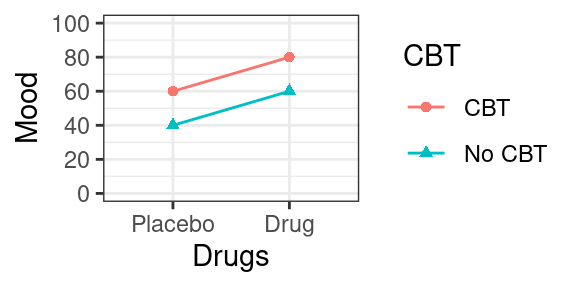
\includegraphics[width=0.5\linewidth]{04-interactions_files/figure-latex/scenario-a-plot-1} 

}

\caption{*Scenario A, plot of cell means.*}\label{fig:scenario-a-plot}
\end{figure}

Below is a table of \textbf{cell means} and \textbf{marginal means}. The cell means are the mean values of the dependent variable (mood) at each cell of the design. The marginal means (in the margins of the table) provide the means for each row and column.

\begin{table}

\caption{\label{tab:scenario-a-means}*Scenario A, Table of Means.*}
\centering
\begin{tabular}[t]{l|r|r|l}
\hline
  & No CBT & CBT &   \\
\hline
Placebo & 40 & 60 & 50\\
\hline
Drug & 60 & 80 & 70\\
\hline
 & 50 & 70 & \\
\hline
\end{tabular}
\end{table}

If this was our outcome, what would you conclude? Is cognitive therapy having an effect on mood? How about drug therapy. The answer to both of these questions is yes: The mean mood for people who got CBT (70; mean of column 2) is 20 points higher than the mean mood for people who didn't (50; mean of column 1).

Likewise, people who got anti-depressants showed enhanced mood (70; mean of row 2) relative to people who got the placebo (50; mean of row 1).

Now we can also ask the following question: \textbf{did the effect of cognitive therapy depend on whether or not the patient was simultaneously receiving drug therapy}? The answer to this, is no. To see why, note that for the Placebo group (Row 1), cognitive therapy increased mood by 20 points (from 40 to 60). But this was the same for the Drug group: there was an increase of 20 points from 60 to 80. So, no evidence that the effect of one factor on mood depends on the other.

\hypertarget{scenario-b}{%
\subsubsection*{Scenario B}\label{scenario-b}}
\addcontentsline{toc}{subsubsection}{Scenario B}

\begin{figure}

{\centering 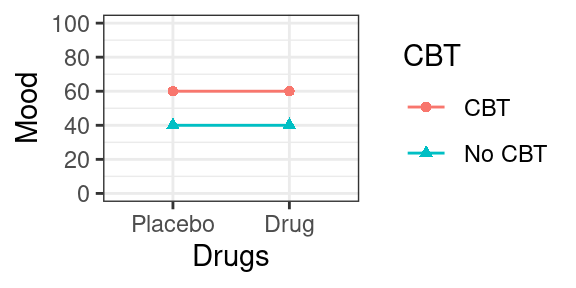
\includegraphics[width=0.5\linewidth]{04-interactions_files/figure-latex/scenario-b-plot-1} 

}

\caption{*Scenario B, plot of cell means.*}\label{fig:scenario-b-plot}
\end{figure}

\begin{table}

\caption{\label{tab:scenario-b-means}*Scenario B, Table of Means.*}
\centering
\begin{tabular}[t]{l|r|r|l}
\hline
  & No CBT & CBT &   \\
\hline
Placebo & 40 & 60 & 50\\
\hline
Drug & 40 & 60 & 50\\
\hline
 & 40 & 60 & \\
\hline
\end{tabular}
\end{table}

In this scenario, we also see that CBT improved mood (again, by 20 points), but there was no effect of Drug Therapy (equal marginal means of 50 for row 1 and row 2). We can also see here that the effect of CBT also didn't depend upon Drug therapy; there is an increase of 20 points in each row.

\hypertarget{scenario-c}{%
\subsubsection*{Scenario C}\label{scenario-c}}
\addcontentsline{toc}{subsubsection}{Scenario C}

\begin{figure}

{\centering 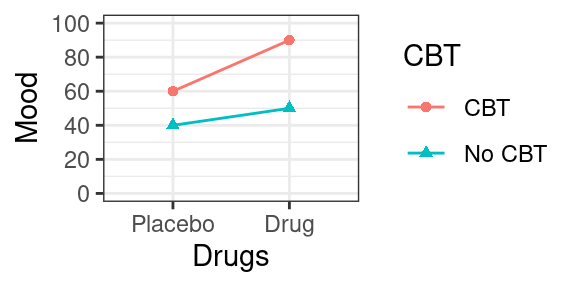
\includegraphics[width=0.5\linewidth]{04-interactions_files/figure-latex/scenario-c-plot-1} 

}

\caption{*Scenario C, plot of cell means.*}\label{fig:scenario-c-plot}
\end{figure}

\begin{table}

\caption{\label{tab:scenario-c-means}*Scenario C, Table of Means.*}
\centering
\begin{tabular}[t]{l|r|r|l}
\hline
  & No CBT & CBT &   \\
\hline
Placebo & 40 & 60 & 50\\
\hline
Drug & 50 & 90 & 70\\
\hline
 & 45 & 75 & \\
\hline
\end{tabular}
\end{table}

Following the logic in previous sections, we see that overall, people who got cognitive therapy showed elevated mood relative to control (75 vs 45), and that people who got drug therapy also showed elevated mood relative to placebo (70 vs 50). But there is something else going on here: it seems that the effect of cognitive therapy on mood was \textbf{more pronounced for patients who were also receiving drug therapy}. For patients on antidepressants, there was a 40 point increase in mood relative to control (from 50 to 90; row 2 of the table). For patients who got the placebo, there was only a 20 point increase in mood, from 40 to 60 (row 1 of the table). So in this hypothetical scenario, \textbf{the effect of cognitive therapy depends on whether or not there is also ongoing drug therapy.}

\hypertarget{effects-in-a-factorial-design}{%
\subsection{Effects in a factorial design}\label{effects-in-a-factorial-design}}

If you understand the basic patterns of effects described in the previous section, you are then ready to map these concepts onto statistical language.

\hypertarget{main-effect}{%
\subsubsection{Main effect}\label{main-effect}}

\textbf{Main effect}: The effect of a factor on the DV \textbf{ignoring} the other factors in the design.

The test of a main effect is a test of the equivalence of marginal means. So in Scenario A above, when you compared the row means for drug therapy, you were assessing the main effect of this factor on mood. The null hypothesis would be that the two marginal means are equal:

\[\bar{Y}_{1..} = \bar{Y}_{2..}\]

where \(Y_{i..}\) is the mean of row \(i\), ignoring the column factor.

If you have a factor with \(k\) levels where \(k > 2\), the null hypothesis for the main effect is

\[\bar{Y}_{1..} = \bar{Y}_{2..} = \ldots = \bar{Y}_{k..},\]

i.e., that all of the row (or column) means are equal.

\hypertarget{simple-effect}{%
\subsubsection{Simple effect}\label{simple-effect}}

A \textbf{Simple effect} is the effect of one factor at a specific level of another factor (i.e., holding that factor constant at a particular value).

So for instance, in Scenario C, we talked about the effect of CBT for participants in the anti-depressant group. In that case, the simple effect of CBT for participants receiving anti-depressants was 40 units.

We could also talk about the simple effect of drug therapy for patients who received cognitive therapy. In Scenario C, this was an increase in mood from 60 to 90 (column 2).

\hypertarget{interaction}{%
\subsubsection{Interaction}\label{interaction}}

We say that an \textbf{interaction} is present when the effect of one variable differs across the levels of another variable.

A more mathematical definition is that an interaction is present when the simple effects of one factor differ across the levels of another factor. We saw this in Scenario C, with a 40 point boost of CBT for the anti-depressant group, compared to a boost of 20 for the placebo group. Perhaps the elevated mood caused by the anti-depressants made patients more susceptable to CBT.

The main point here is that we say there is a simple interaction between A and B when the simple effects of A differ across the levels of B. You could also check whether the simple effects of B differ across A. It is not possible for one of these statements to be true without the other also being true, so it doesn't matter which way you look at the simple effects.

\hypertarget{higher-order-designs}{%
\subsection{Higher-order designs}\label{higher-order-designs}}

Two-factor (also known as ``two-way'') designs are very common in psychology and neuroscience, but sometimes you will also see designs with more than two factors, such as a 2x2x2 design.

To figure out the number of effects we have of different kinds, we use the formula below, which gives us the number of possible combinations for \(n\) elements take \(k\) at a time:

\[\frac{n!}{k!(n - k)!}\]

Rather than actually computing this by hand, we can just use the \texttt{choose(n,\ k)} function in R.

For any design with \(n\) factors, you will have:

\begin{itemize}
\tightlist
\item
  \(n\) main effects;
\item
  \(\frac{n!}{2!(n - 2)!}\) two-way interactions;
\item
  \(\frac{n!}{3!(n - 3)!}\) three-way interactions;
\item
  \(\frac{n!}{4!(n - 4)!}\) four-way interactions\ldots{} and so forth.
\end{itemize}

So if we have a three-way design, e.g., a 2x2x2 with factors \(A\), \(B\), and \(C\), we would have 3 main effects: \(A\), \(B\), and \(C\). We would have \texttt{choose(3,\ 2)} = three two way interactions: \(AB\), \(AC\), and \(BC\), and \texttt{choose(3,\ 3)} = one three-way interaction: \(ABC\).

Three-way interactions are hard to interpret, but what they imply is that the \textbf{simple interaction} between any two given factors varies across the level of the third factor. For example, it would imply that the \(AB\) interaction at \(C_1\) would be different from the \(AB\) interaction at \(C_2\).

If you have a four way design, you have four main effects, \texttt{choose(4,\ 2)\ =}6 two-way interactions, \texttt{choose(4,\ 3)\ =}4 three-way interactions, and one four-way interaction. It is next to impossible to interpret results from a four-way design, so keep your designs simple!

\hypertarget{the-glm-for-a-factorial-design}{%
\section{The GLM for a factorial design}\label{the-glm-for-a-factorial-design}}

Now let's look at the math behind these models. The typically way you'll see the GLM for an ANOVA written for a 2x2 factorial design uses ``ANOVA'' notation, like so:

\[Y_{ijk} = \mu + A_i + B_j + AB_{ij} + S(AB)_{ijk}.\]

In the above formula,

\begin{itemize}
\tightlist
\item
  \(Y_{ijk}\) is the score for observation \(k\) at level \(i\) of \(A\) and level \(j\) of \(B\);
\item
  \(\mu\) is the grand mean;
\item
  \(A_i\) is the main effect of factor \(A\) at level \(i\) of \(A\);
\item
  \(B_j\) is the main effect of factor \(B\) at level \(j\) of \(B\);
\item
  \(AB_{ij}\) is the \(AB\) interaction at level \(i\) of \(A\) and level \(j\) of \(B\);
\item
  \(S(AB)_{ijk}\) is the residual.
\end{itemize}

An important mathematical fact is that the individual main and interaction effects sum to zero, often written as:

\begin{itemize}
\tightlist
\item
  \(\Sigma_i A_i = 0\);
\item
  \(\Sigma_j B_j = 0\);
\item
  \(\Sigma_{ij} AB_{ij} = 0\).
\end{itemize}

The best way to understand these effects is to see them in a decomposition table. Study the decomposition table belo wfor 12 simulated observations from a 2x2 design with factors \(A\) and \(B\). The indexes \(i\), \(j\), and \(k\) are provided just to help you keep track of what observation you are dealing with. Remember that \(i\) indexes the level of factor \(A\), \(j\) indexes the level of factor \(B\), and \(k\) indexes the observation number within the cell \(AB_{ij}\).

\begin{verbatim}
## # A tibble: 12 x 9
##        Y     i     j     k    mu   A_i   B_j AB_ij   err
##    <dbl> <int> <int> <int> <dbl> <dbl> <dbl> <dbl> <int>
##  1    11     1     1     1    10     4    -2    -1     0
##  2    14     1     1     2    10     4    -2    -1     3
##  3     8     1     1     3    10     4    -2    -1    -3
##  4    17     1     2     1    10     4     2     1     0
##  5    15     1     2     2    10     4     2     1    -2
##  6    19     1     2     3    10     4     2     1     2
##  7     8     2     1     1    10    -4    -2     1     3
##  8     4     2     1     2    10    -4    -2     1    -1
##  9     3     2     1     3    10    -4    -2     1    -2
## 10    10     2     2     1    10    -4     2    -1     3
## 11     7     2     2     2    10    -4     2    -1     0
## 12     4     2     2     3    10    -4     2    -1    -3
\end{verbatim}

\hypertarget{estimation-equations}{%
\subsection{Estimation equations}\label{estimation-equations}}

These are the equations you would used to estimate effects in an ANOVA.

\begin{itemize}
\tightlist
\item
  \(\hat{\mu} = Y_{...}\)
\item
  \(\hat{A}_i = Y_{i..} - \hat{\mu}\)
\item
  \(\hat{B}_j = Y_{.j.} - \hat{\mu}\)
\item
  \(\widehat{AB}_{ij} = Y_{ij.} - \hat{\mu} - \hat{A}_i - \hat{B}_j\)
\end{itemize}

Note that the \(Y\) variable with the dots in the subscripts are means of \(Y\), taken while ignoring anything appearing as a dot. So \(Y_{...}\) is mean of \(Y\), \(Y_{i..}\) is the mean of \(Y\) at level \(i\) of \(A\), \(Y_{.j.}\) is the mean of \(Y\) at level \(j\) of \(B\), and \(Y_{ij.}\) is the mean of \(Y\) at level \(i\) of \(A\) and level \(j\) of \(B\), i.e., the cell mean \(ij\).

\hypertarget{factorial-app}{%
\subsection{Factorial App}\label{factorial-app}}

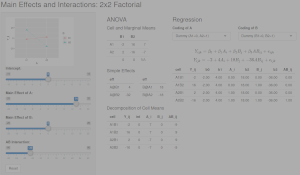
\includegraphics{images/04-interactions_factorial_app.png}

\href{https://shiny.psy.gla.ac.uk/Dale/factorial2}{Launch this web application} and experiment with factorial designs until you understand the key concepts of main effects and interactions in a factorial design.

\hypertarget{code-your-own-categorical-predictors-in-factorial-designs}{%
\section{Code your own categorical predictors in factorial designs}\label{code-your-own-categorical-predictors-in-factorial-designs}}

Many studies in psychology---especially experimental psychology---involve categorical independent variables. Analyzing data from these studies requires care in specifying the predictors, because the defaults in R are not ideal for experimental situations.

Let's say you have 2x2 designed experiment with factors priming condition (priming vs.~no priming) and linguistic structure (noun vs verb). These columns can be represented as type \texttt{character} or \texttt{factor}; in the latter case, they are implicitly converted to type \texttt{factor} before fitting the model, and then R will apply the default numerical coding for factors, which is `treatment' (0, 1) coding.

If you're used to running ANOVAs, the results that you get from fitting a linear model will \emph{not} match ANOVA output, as we'll see below. That is because you need to use a different coding scheme to get ANOVA-like output.

First, let's define our little data set, \texttt{dat}.

\begin{Shaded}
\begin{Highlighting}[]
  \CommentTok{## demo for why you should avoid factors}
\NormalTok{  dat <-}\StringTok{ }\KeywordTok{tibble}\NormalTok{(}
    \DataTypeTok{subject =} \KeywordTok{factor}\NormalTok{(}\DecValTok{1}\OperatorTok{:}\DecValTok{16}\NormalTok{),}
    \DataTypeTok{priming =} \KeywordTok{rep}\NormalTok{(}\KeywordTok{c}\NormalTok{(}\StringTok{"yes"}\NormalTok{, }\StringTok{"no"}\NormalTok{), }\DataTypeTok{each =} \DecValTok{8}\NormalTok{),}
    \DataTypeTok{structure =} \KeywordTok{rep}\NormalTok{(}\KeywordTok{rep}\NormalTok{(}\KeywordTok{c}\NormalTok{(}\StringTok{"noun"}\NormalTok{, }\StringTok{"verb"}\NormalTok{), }\DataTypeTok{each =} \DecValTok{4}\NormalTok{), }\DecValTok{2}\NormalTok{),}
    \DataTypeTok{RT =} \KeywordTok{rnorm}\NormalTok{(}\DecValTok{16}\NormalTok{, }\DecValTok{800}\NormalTok{, }\DecValTok{20}\NormalTok{))}

\NormalTok{  dat}
\end{Highlighting}
\end{Shaded}

\begin{verbatim}
## # A tibble: 16 x 4
##    subject priming structure    RT
##    <fct>   <chr>   <chr>     <dbl>
##  1 1       yes     noun       792.
##  2 2       yes     noun       771.
##  3 3       yes     noun       760.
##  4 4       yes     noun       811.
##  5 5       yes     verb       787.
##  6 6       yes     verb       820.
##  7 7       yes     verb       768.
##  8 8       yes     verb       806.
##  9 9       no      noun       791.
## 10 10      no      noun       824.
## 11 11      no      noun       817.
## 12 12      no      noun       790.
## 13 13      no      verb       790.
## 14 14      no      verb       813.
## 15 15      no      verb       810.
## 16 16      no      verb       763.
\end{verbatim}

This is between subjects data, so we can fit a model using \texttt{lm()}. In the model, we include effects of \texttt{priming} and \texttt{structure} as well as their interaction. Instead of typing \texttt{priming\ +\ structure\ +\ priming:structure} we can simply type the shortcut \texttt{priming\ *\ structure}.

\begin{Shaded}
\begin{Highlighting}[]
\NormalTok{  ps_mod <-}\StringTok{ }\KeywordTok{lm}\NormalTok{(RT }\OperatorTok{~}\StringTok{ }\NormalTok{priming }\OperatorTok{*}\StringTok{ }\NormalTok{structure, dat)}

  \KeywordTok{summary}\NormalTok{(ps_mod)}
\end{Highlighting}
\end{Shaded}

\begin{verbatim}
## 
## Call:
## lm(formula = RT ~ priming * structure, data = dat)
## 
## Residuals:
##     Min      1Q  Median      3Q     Max 
## -30.782 -14.711   2.036  16.466  27.755 
## 
## Coefficients:
##                          Estimate Std. Error t value Pr(>|t|)    
## (Intercept)                805.57      10.83  74.409   <2e-16 ***
## primingyes                 -22.08      15.31  -1.442    0.175    
## structureverb              -11.49      15.31  -0.750    0.468    
## primingyes:structureverb    23.20      21.65   1.071    0.305    
## ---
## Signif. codes:  0 '***' 0.001 '**' 0.01 '*' 0.05 '.' 0.1 ' ' 1
## 
## Residual standard error: 21.65 on 12 degrees of freedom
## Multiple R-squared:  0.1481,	Adjusted R-squared:  -0.06493 
## F-statistic: 0.6951 on 3 and 12 DF,  p-value: 0.5726
\end{verbatim}

Note that in the output the predictors are shown as \texttt{primingyes} and \texttt{structureverb}. The value \texttt{yes} is a level of \texttt{priming}; the level \textbf{not shown} is the one chosen as baseline, and in the default treatment coding scheme, the not-shown level (\texttt{no}) is coded as 0, and the shown level (\texttt{yes}) is coded as 1. Likewise, for \texttt{structure}, \texttt{noun} is coded as 0 and \texttt{verb} is coded as 1.

This is not ideal, for reasons we will discuss further below. But I want to show you a further quirk of using factor variables as predictors.

Let's say we wanted to test the effect of \texttt{priming} by itself using model comparison. To do this, we would fit another model where we exclude this effect while keeping the interaction. Despite what you may have heard to the contrary, in a fully randomized, balanced experiment, all factors are orthogonal, and so it is completely legitimate to drop a main effect while leaving an interaction term in the model.

\begin{Shaded}
\begin{Highlighting}[]
\NormalTok{  ps_mod_nopriming <-}\StringTok{ }\KeywordTok{lm}\NormalTok{(RT }\OperatorTok{~}\StringTok{ }\NormalTok{structure }\OperatorTok{+}\StringTok{ }\NormalTok{priming}\OperatorTok{:}\NormalTok{structure, dat)}
\end{Highlighting}
\end{Shaded}

OK, now that we've dropped \texttt{priming}, we should have 3 parameter estimates instead of 4. Let's check.

\begin{Shaded}
\begin{Highlighting}[]
  \CommentTok{## not right!}
  \KeywordTok{coef}\NormalTok{(ps_mod_nopriming)}
\end{Highlighting}
\end{Shaded}

\begin{verbatim}
##              (Intercept)            structureverb structurenoun:primingyes 
##               805.566187               -11.485457               -22.081224 
## structureverb:primingyes 
##                 1.117333
\end{verbatim}

There are still 4 of them, and we're suddenly getting \texttt{primingyes:structureverb}. This is weird and \emph{not at all} what we intended. If we try to do the model comparison:

\begin{Shaded}
\begin{Highlighting}[]
  \CommentTok{## nonsense result}
  \KeywordTok{anova}\NormalTok{(ps_mod_nopriming, ps_mod)}
\end{Highlighting}
\end{Shaded}

\begin{verbatim}
## Analysis of Variance Table
## 
## Model 1: RT ~ structure + priming:structure
## Model 2: RT ~ priming * structure
##   Res.Df  RSS Df  Sum of Sq F Pr(>F)
## 1     12 5626                       
## 2     12 5626  0 9.0949e-13
\end{verbatim}

we'd get nonsensical results.

Is this a bug? No.~It was a (in my view, heavy handed) design choice by the R creators to try to prevent everyone from doing something that at least some of us should be able to do at least some of the time.

But we can do whatever we please if instead of using factors we define our own numerical predictors. This adds a bit of work but avoids other headaches and mistakes that we might make by using factors. Also, being very explicit about how predictors are defined is probably a good thing.

You'll sometimes need \texttt{factor} variables. I often use them to get things to plot in the right way using \texttt{ggplot2}, or when I need to tabulating observations and there are some combinations with zero counts. But I recommend against using \texttt{factors} in statistical models, especially if your model includes interactions. Use numerical predictors instead.

\hypertarget{coding-schemes-for-categorical-variables}{%
\section{Coding schemes for categorical variables}\label{coding-schemes-for-categorical-variables}}

Many experimentalists who are trying to make the leap from ANOVA to linear mixed-effects models (LMEMs) in R struggle with the coding of categorical predictors. It is unexpectedly complicated, and the defaults provided in R turn out to be wholly inappropriate for factorial experiments. Indeed, using those defaults with factorial experiments can lead researchers to draw erroneous conclusions from their data.

To keep things simple, we'll start with situations where design factors have no more than two levels before moving on to designs with more than three levels.

\hypertarget{simple-versus-main-effects}{%
\subsection{Simple versus main effects}\label{simple-versus-main-effects}}

It is important that you understand the difference between a \textbf{simple effect} and a \textbf{main effect}, and between a \textbf{simple interaction} and a \textbf{main interaction} in a three-way design.

In an \(A{\times}B\) design, the simple effect of \(A\) is the effect of \(A\) \textbf{controlling} for \(B\), while the main effect of \(A\) is the effect of \(A\) \textbf{ignoring} \(B\). Another way of looking at this is to consider the cell means (\(\bar{Y}_{11}\), \(\bar{Y}_{12}\), \(\bar{Y}_{21}\), and \(\bar{Y}_{22}\)) and marginal means (\(\bar{Y}_{1.}\), \(\bar{Y}_{2.}\), \(\bar{Y}_{.1}\), and \(\bar{Y}_{.2}\)) in a factorial design. (The dot subscript tells you to ``ignore'' the dimension containing the dot; e.g., \(\bar{Y}_{.1}\) tells you to take the mean of the first column ignoring the row variable.) To test the main effect of A is to test the null hypothesis that \(\bar{Y}_{1.}=\bar{Y}_{2.}\). To test a simple effect of \(A\)---the effect of \(A\) at a particular level of \(B\)---would be, for instance, to test the null hypothesis that \(\bar{Y}_{11}=\bar{Y}_{21}\).

\begin{table}[H]
\centering
\begin{tabular}{c|c|c|c|c}
\hline
 & \textbackslash{}(B\_1\textbackslash{}) & \textbackslash{}(B\_2\textbackslash{}) &  & \\
\hline
\textbackslash{}(A\_1\textbackslash{}) & \$\textbackslash{}bar\{Y\}\_\{11\}\$ & \$\textbackslash{}bar\{Y\}\_\{12\}\$ &  & \$\textbackslash{}bar\{Y\}\_\{1.\}\$\\
\hline
\textbackslash{}(A\_2\textbackslash{}) & \$\textbackslash{}bar\{Y\}\_\{21\}\$ & \$\textbackslash{}bar\{Y\}\_\{22\}\$ &  & \$\textbackslash{}bar\{Y\}\_\{2.\}\$\\
\hline
 &  &  &  & \\
\hline
 & \$\textbackslash{}bar\{Y\}\_\{.1\}\$ & \$\textbackslash{}bar\{Y\}\_\{.2\}\$ &  & \\
\hline
\end{tabular}
\end{table}

The distinction between \textbf{simple interactions} and \textbf{main interactions} has the same logic: the simple interaction of \(AB\) in an \(ABC\) design is the interaction of \(AB\) at a particular level of \(C\); the main interaction of \(AB\) is the interaction \textbf{ignoring} C. The latter is what we are usually talking about when we talk about lower-order interactions in a three-way design. It is also what we are given in the output from standard ANOVA procedures, e.g., the \texttt{aov()} function in R, SPSS, SAS, etc.

\hypertarget{the-key-coding-schemes}{%
\subsection{The key coding schemes}\label{the-key-coding-schemes}}

Generally, the choice of a coding scheme impacts the interpretation of:

\begin{enumerate}
\def\labelenumi{\arabic{enumi}.}
\tightlist
\item
  the intercept term; and
\item
  the interpretation of the tests for all but the highest-order effects and interactions in a factorial design.
\end{enumerate}

It also can influence the interpretation/estimation of random effects in a mixed-effects model (see \href{https://talklab.psy.gla.ac.uk/simgen/rsonly.html}{this blog post} for further discussion). If you have a design with only a single two-level factor, and are using a \href{https://www.sciencedirect.com/science/article/pii/S0749596X12001180}{maximal random-effects structure}, the choice of coding scheme doesn't really matter.

There are many possible coding schemes (see \texttt{?contr.treatment} for more information). The most relevant ones are \textbf{treatment}, \textbf{sum}, and \textbf{deviation}. Sum and deviation coding can be seen as special cases of \textbf{effect} coding; by effect coding, people generally mean codes that sum to zero.

For a two-level factor, you would use the following codes:

\begin{table}[H]
\centering
\begin{tabular}{l|r|r}
\hline
Scheme & \textbackslash{}(A\_1\textbackslash{}) & \textbackslash{}(A\_2\textbackslash{})\\
\hline
Treatment (dummy) & \textbackslash{}(0\textbackslash{}) & \textbackslash{}(1\textbackslash{})\\
\hline
Sum & \textbackslash{}(-1\textbackslash{}) & \textbackslash{}(1\textbackslash{})\\
\hline
Deviation & \textbackslash{}(-\textbackslash{}frac\{1\}\{2\}\textbackslash{}) & \textbackslash{}(\textbackslash{}frac\{1\}\{2\}\textbackslash{})\\
\hline
\end{tabular}
\end{table}

\begin{description}
\item[The default in R is to use treatment coding for any variable defined as a =factor= in the model (see \texttt{?factor} and \texttt{?contrasts} for information). To see why this is not ideal for factorial designs, consider a 2x2x2 factorial design with factors \(A\), \(B\) and \(C\). We will just consider a fully between-subjects design with only one observation per subject as this allows us to use the simplest possible error structure. We would fit such a model using \texttt{lm()}:]
lm(Y \textasciitilde{} A * B * C)
\end{description}

The figure below spells out the notation for the various cell and marginal means for a 2x2x2 design.

\[C_1\]

\begin{table}[H]
\centering
\begin{tabular}{c|c|c|c|c}
\hline
 & \textbackslash{}(B\_1\textbackslash{}) & \textbackslash{}(B\_2\textbackslash{}) &  & \\
\hline
\textbackslash{}(A\_1\textbackslash{}) & \$\textbackslash{}bar\{Y\}\_\{111\}\$ & \$\textbackslash{}bar\{Y\}\_\{121\}\$ &  & \$\textbackslash{}bar\{Y\}\_\{1.1\}\$\\
\hline
\textbackslash{}(A\_2\textbackslash{}) & \$\textbackslash{}bar\{Y\}\_\{211\}\$ & \$\textbackslash{}bar\{Y\}\_\{221\}\$ &  & \$\textbackslash{}bar\{Y\}\_\{2.1\}\$\\
\hline
 &  &  &  & \\
\hline
 & \$\textbackslash{}bar\{Y\}\_\{.11\}\$ & \$\textbackslash{}bar\{Y\}\_\{.21\}\$ &  & \\
\hline
\end{tabular}
\end{table}

\[C_2\]

\begin{table}[H]
\centering
\begin{tabular}{c|c|c|c|c}
\hline
 & \textbackslash{}(B\_1\textbackslash{}) & \textbackslash{}(B\_2\textbackslash{}) &  & \\
\hline
\textbackslash{}(A\_1\textbackslash{}) & \$\textbackslash{}bar\{Y\}\_\{112\}\$ & \$\textbackslash{}bar\{Y\}\_\{122\}\$ &  & \$\textbackslash{}bar\{Y\}\_\{1.2\}\$\\
\hline
\textbackslash{}(A\_2\textbackslash{}) & \$\textbackslash{}bar\{Y\}\_\{212\}\$ & \$\textbackslash{}bar\{Y\}\_\{222\}\$ &  & \$\textbackslash{}bar\{Y\}\_\{2.2\}\$\\
\hline
 &  &  &  & \\
\hline
 & \$\textbackslash{}bar\{Y\}\_\{.12\}\$ & \$\textbackslash{}bar\{Y\}\_\{.22\}\$ &  & \\
\hline
\end{tabular}
\end{table}

The table below provides the interpretation for various effects in the model under the three different coding schemes. Note that \(Y\) is the dependent variable, and the dots in the subscript mean to ``ignore'' the corresponding dimension. Thus, \(\bar{Y}_{.1.}\) is the mean of B\_1 (ignoring factors \(A\) and \(C\)) and \(\bar{Y}_{...}\) is the ``grand mean'' (ignoring all factors).

\begin{table}[H]
\centering
\begin{tabular}{c|c|c|c}
\hline
term & treatment & sum & deviation\\
\hline
\textbackslash{}(\textbackslash{}mu\textbackslash{}) & \$\textbackslash{}bar\{Y\}\_\{111\}\$ & \$\textbackslash{}bar\{Y\}\_\{...\}\$ & \$\textbackslash{}bar\{Y\}\_\{...\}\$\\
\hline
\textbackslash{}(A\textbackslash{}) & \textbackslash{}(\textbackslash{}bar\{Y\}\_\{211\} - \textbackslash{}bar\{Y\}\_\{111\}\textbackslash{}) & \textbackslash{}(\textbackslash{}frac\{(\textbackslash{}bar\{Y\}\_\{2..\} - \textbackslash{}bar\{Y\}\_\{1..\})\}\{2\}\textbackslash{}) & \textbackslash{}(\textbackslash{}bar\{Y\}\_\{2..\} - \textbackslash{}bar\{Y\}\_\{1..\}\textbackslash{})\\
\hline
\textbackslash{}(B\textbackslash{}) & \textbackslash{}(\textbackslash{}bar\{Y\}\_\{121\} - \textbackslash{}bar\{Y\}\_\{111\}\textbackslash{}) & \textbackslash{}(\textbackslash{}frac\{(\textbackslash{}bar\{Y\}\_\{.2.\} - \textbackslash{}bar\{Y\}\_\{.1.\})\}\{2\}\textbackslash{}) & \textbackslash{}(\textbackslash{}bar\{Y\}\_\{.2.\} - \textbackslash{}bar\{Y\}\_\{.1.\}\textbackslash{})\\
\hline
\textbackslash{}(C\textbackslash{}) & \textbackslash{}(\textbackslash{}bar\{Y\}\_\{112\} - \textbackslash{}bar\{Y\}\_\{111\}\textbackslash{}) & \textbackslash{}(\textbackslash{}frac\{(\textbackslash{}bar\{Y\}\_\{..2\} - \textbackslash{}bar\{Y\}\_\{..1\})\}\{2\}\textbackslash{}) & \textbackslash{}(\textbackslash{}bar\{Y\}\_\{..2\} - \textbackslash{}bar\{Y\}\_\{..1\}\textbackslash{})\\
\hline
\textbackslash{}(AB\textbackslash{}) & \textbackslash{}((\textbackslash{}bar\{Y\}\_\{221\} - \textbackslash{}bar\{Y\}\_\{121\}) - (\textbackslash{}bar\{Y\}\_\{211\} - \textbackslash{}bar\{Y\}\_\{111\})\textbackslash{}) & \textbackslash{}(\textbackslash{}frac\{(\textbackslash{}bar\{Y\}\_\{22.\} - \textbackslash{}bar\{Y\}\_\{12.\}) - (\textbackslash{}bar\{Y\}\_\{21.\} - \textbackslash{}bar\{Y\}\_\{11.\})\}\{4\}\textbackslash{}) & \textbackslash{}((\textbackslash{}bar\{Y\}\_\{22.\} - \textbackslash{}bar\{Y\}\_\{12.\}) - (\textbackslash{}bar\{Y\}\_\{21.\} - \textbackslash{}bar\{Y\}\_\{11.\})\textbackslash{})\\
\hline
\textbackslash{}(AC\textbackslash{}) & \textbackslash{}((\textbackslash{}bar\{Y\}\_\{212\} - \textbackslash{}bar\{Y\}\_\{211\}) - (\textbackslash{}bar\{Y\}\_\{112\} - \textbackslash{}bar\{Y\}\_\{111\})\textbackslash{}) & \textbackslash{}(\textbackslash{}frac\{(\textbackslash{}bar\{Y\}\_\{2.2\} - \textbackslash{}bar\{Y\}\_\{1.2\}) - (\textbackslash{}bar\{Y\}\_\{2.1\} - \textbackslash{}bar\{Y\}\_\{1.1\})\}\{4\}\textbackslash{}) & \textbackslash{}((\textbackslash{}bar\{Y\}\_\{2.2\} - \textbackslash{}bar\{Y\}\_\{1.2\}) - (\textbackslash{}bar\{Y\}\_\{2.1\} - \textbackslash{}bar\{Y\}\_\{1.1\})\textbackslash{})\\
\hline
\textbackslash{}(BC\textbackslash{}) & \textbackslash{}((\textbackslash{}bar\{Y\}\_\{122\} - \textbackslash{}bar\{Y\}\_\{112\}) - (\textbackslash{}bar\{Y\}\_\{121\} - \textbackslash{}bar\{Y\}\_\{111\})\textbackslash{}) & \textbackslash{}(\textbackslash{}frac\{(\textbackslash{}bar\{Y\}\_\{.22\} - \textbackslash{}bar\{Y\}\_\{.12\}) - (\textbackslash{}bar\{Y\}\_\{.21\} - \textbackslash{}bar\{Y\}\_\{.11\})\}\{4\}\textbackslash{}) & \textbackslash{}((\textbackslash{}bar\{Y\}\_\{.22\} - \textbackslash{}bar\{Y\}\_\{.12\}) - (\textbackslash{}bar\{Y\}\_\{.21\} - \textbackslash{}bar\{Y\}\_\{.11\})\textbackslash{})\\
\hline
\end{tabular}
\end{table}

For the three way \(A \times B \times C\) interaction:

\begin{table}[H]
\centering
\begin{tabular}{c|c}
\hline
scheme & interpretation\\
\hline
treatment & \textbackslash{}(\textbackslash{}displaystyle\textbackslash{}left[\textbackslash{}displaystyle\textbackslash{}left(\textbackslash{}bar\{Y\}\_\{221\} - \textbackslash{}bar\{Y\}\_\{121\}\textbackslash{}right) - \textbackslash{}displaystyle\textbackslash{}left(\textbackslash{}bar\{Y\}\_\{211\} - \textbackslash{}bar\{Y\}\_\{111\}\textbackslash{}right)\textbackslash{}right] - \textbackslash{}displaystyle\textbackslash{}left[\textbackslash{}displaystyle\textbackslash{}left(\textbackslash{}bar\{Y\}\_\{222\} - \textbackslash{}bar\{Y\}\_\{122\}\textbackslash{}right) - \textbackslash{}displaystyle\textbackslash{}left(\textbackslash{}bar\{Y\}\_\{212\} - \textbackslash{}bar\{Y\}\_\{112\}\textbackslash{}right)\textbackslash{}right]\textbackslash{})\\
\hline
sum & \textbackslash{}(\textbackslash{}frac\{\textbackslash{}displaystyle\textbackslash{}left[\textbackslash{}displaystyle\textbackslash{}left(\textbackslash{}bar\{Y\}\_\{221\} - \textbackslash{}bar\{Y\}\_\{121\}\textbackslash{}right) - \textbackslash{}displaystyle\textbackslash{}left(\textbackslash{}bar\{Y\}\_\{211\} - \textbackslash{}bar\{Y\}\_\{111\}\textbackslash{}right)\textbackslash{}right] - \textbackslash{}displaystyle\textbackslash{}left[\textbackslash{}displaystyle\textbackslash{}left(\textbackslash{}bar\{Y\}\_\{222\} - \textbackslash{}bar\{Y\}\_\{122\}\textbackslash{}right) - \textbackslash{}displaystyle\textbackslash{}left(\textbackslash{}bar\{Y\}\_\{212\} - \textbackslash{}bar\{Y\}\_\{112\}\textbackslash{}right)\textbackslash{}right]\}\{8\}\textbackslash{})\\
\hline
deviation & \textbackslash{}(\textbackslash{}displaystyle\textbackslash{}left[\textbackslash{}displaystyle\textbackslash{}left(\textbackslash{}bar\{Y\}\_\{221\} - \textbackslash{}bar\{Y\}\_\{121\}\textbackslash{}right) - \textbackslash{}displaystyle\textbackslash{}left(\textbackslash{}bar\{Y\}\_\{211\} - \textbackslash{}bar\{Y\}\_\{111\}\textbackslash{}right)\textbackslash{}right] - \textbackslash{}displaystyle\textbackslash{}left[\textbackslash{}displaystyle\textbackslash{}left(\textbackslash{}bar\{Y\}\_\{222\} - \textbackslash{}bar\{Y\}\_\{122\}\textbackslash{}right) - \textbackslash{}displaystyle\textbackslash{}left(\textbackslash{}bar\{Y\}\_\{212\} - \textbackslash{}bar\{Y\}\_\{112\}\textbackslash{}right)\textbackslash{}right]\textbackslash{})\\
\hline
\end{tabular}
\end{table}

Note that the inferential tests of \(A \times B \times C\) will all have the same outcome, despite the parameter estimate for sum coding being one-eighth of that for the other schemes. For all lower-order effects, sum and deviation coding will give different parameter estimates but identical inferential outcomes. Both of these schemes provide identical tests of the canonical main effects and main interactions for a three-way ANOVA. In contrast, treatment (dummy) coding will provide inferential tests of simple effects and simple interactions. So, if what you are interested in getting are the ``canonical'' tests from ANOVA, use sum or deviation coding.

\hypertarget{what-about-factors-with-more-than-two-levels}{%
\subsection{What about factors with more than two levels?}\label{what-about-factors-with-more-than-two-levels}}

A factor with \(k\) levels requires \(k-1\) variables. Each predictor contrasts a particular ``target'' level of the factor with a level that you (arbitrarily) choose as the ``baseline'' level. For instance, for a three-level factor \(A\) with \(A1\) chosen as the baseline, you'd have two predictor variables, one of which compares \(A2\) to \(A1\) and the other of which compares \(A3\) to \(A1\).

For treatment (dummy) coding, the target level is set to 1, otherwise 0.

For sum coding, the levels must sum to zero, so for a given predictor, the target level is given the value 1, the baseline level is given the value -1, and any other level is given the value 0.

For deviation coding, the values must also sum to 0. Deviation coding is recommended whenever you are trying to draw ANOVA-style inferences. Under this scheme, the target level gets the value \(\frac{k-1}{k}\) while any non-target level gets the value \(-\frac{1}{k}\).

\textbf{Fun fact}: Mean-centering treatment codes (on balanced data) will give you deviation codes.

\hypertarget{example-three-level-factor}{%
\subsection{Example: Three-level factor}\label{example-three-level-factor}}

\hypertarget{treatment-dummy}{%
\subsubsection{Treatment (Dummy)}\label{treatment-dummy}}

\begin{table}[H]
\centering
\begin{tabular}{l|r|r}
\hline
level & A2v1 & A3v1\\
\hline
A1 & 0 & 0\\
\hline
A2 & 1 & 0\\
\hline
A3 & 0 & 1\\
\hline
\end{tabular}
\end{table}

\hypertarget{sum}{%
\subsubsection{Sum}\label{sum}}

\begin{table}[H]
\centering
\begin{tabular}{l|r|r}
\hline
level & A2v1 & A3v1\\
\hline
A1 & -1 & -1\\
\hline
A2 & 1 & 0\\
\hline
A3 & 0 & 1\\
\hline
\end{tabular}
\end{table}

\hypertarget{deviation}{%
\subsubsection{Deviation}\label{deviation}}

\begin{table}[H]
\centering
\begin{tabular}{l|r|r}
\hline
level & A2v1 & A3v1\\
\hline
A1 & \textbackslash{}(-\textbackslash{}frac\{1\}\{3\}\textbackslash{}) & \textbackslash{}(-\textbackslash{}frac\{1\}\{3\}\textbackslash{})\\
\hline
A2 & \textbackslash{}(\textbackslash{}frac\{2\}\{3\}\textbackslash{}) & \textbackslash{}(-\textbackslash{}frac\{1\}\{3\}\textbackslash{})\\
\hline
A3 & \textbackslash{}(-\textbackslash{}frac\{1\}\{3\}\textbackslash{}) & \textbackslash{}(\textbackslash{}frac\{2\}\{3\}\textbackslash{})\\
\hline
\end{tabular}
\end{table}

\hypertarget{example-five-level-factor}{%
\subsubsection{Example: Five-level factor}\label{example-five-level-factor}}

\hypertarget{treatment-dummy-1}{%
\subsubsection{Treatment (Dummy)}\label{treatment-dummy-1}}

\begin{table}[H]
\centering
\begin{tabular}{l|r|r|r|r}
\hline
level & A2v1 & A3v1 & A4v1 & A5v1\\
\hline
A1 & 0 & 0 & 0 & 0\\
\hline
A2 & 1 & 0 & 0 & 0\\
\hline
A3 & 0 & 1 & 0 & 0\\
\hline
A4 & 0 & 0 & 1 & 0\\
\hline
A5 & 0 & 0 & 0 & 1\\
\hline
\end{tabular}
\end{table}

\hypertarget{sum-1}{%
\subsubsection{Sum}\label{sum-1}}

\begin{table}[H]
\centering
\begin{tabular}{l|r|r|r|r}
\hline
level & A2v1 & A3v1 & A4v1 & A5v1\\
\hline
A1 & -1 & -1 & -1 & -1\\
\hline
A2 & 1 & 0 & 0 & 0\\
\hline
A3 & 0 & 1 & 0 & 0\\
\hline
A4 & 0 & 0 & 1 & 0\\
\hline
A5 & 0 & 0 & 0 & 1\\
\hline
\end{tabular}
\end{table}

\hypertarget{deviation-1}{%
\subsubsection{Deviation}\label{deviation-1}}

\begin{table}[H]
\centering
\begin{tabular}{l|r|r|r|r}
\hline
level & A2v1 & A3v1 & A4v1 & A5v1\\
\hline
A1 & \textbackslash{}(-\textbackslash{}frac\{1\}\{5\}\textbackslash{}) & \textbackslash{}(-\textbackslash{}frac\{1\}\{5\}\textbackslash{}) & \textbackslash{}(-\textbackslash{}frac\{1\}\{5\}\textbackslash{}) & \textbackslash{}(-\textbackslash{}frac\{1\}\{5\}\textbackslash{})\\
\hline
A2 & \textbackslash{}(\textbackslash{}frac\{4\}\{5\}\textbackslash{}) & \textbackslash{}(-\textbackslash{}frac\{1\}\{5\}\textbackslash{}) & \textbackslash{}(-\textbackslash{}frac\{1\}\{5\}\textbackslash{}) & \textbackslash{}(-\textbackslash{}frac\{1\}\{5\}\textbackslash{})\\
\hline
A3 & \textbackslash{}(-\textbackslash{}frac\{1\}\{5\}\textbackslash{}) & \textbackslash{}(\textbackslash{}frac\{4\}\{5\}\textbackslash{}) & \textbackslash{}(-\textbackslash{}frac\{1\}\{5\}\textbackslash{}) & \textbackslash{}(-\textbackslash{}frac\{1\}\{5\}\textbackslash{})\\
\hline
A4 & \textbackslash{}(-\textbackslash{}frac\{1\}\{5\}\textbackslash{}) & \textbackslash{}(-\textbackslash{}frac\{1\}\{5\}\textbackslash{}) & \textbackslash{}(\textbackslash{}frac\{4\}\{5\}\textbackslash{}) & \textbackslash{}(-\textbackslash{}frac\{1\}\{5\}\textbackslash{})\\
\hline
A5 & \textbackslash{}(-\textbackslash{}frac\{1\}\{5\}\textbackslash{}) & \textbackslash{}(-\textbackslash{}frac\{1\}\{5\}\textbackslash{}) & \textbackslash{}(-\textbackslash{}frac\{1\}\{5\}\textbackslash{}) & \textbackslash{}(\textbackslash{}frac\{4\}\{5\}\textbackslash{})\\
\hline
\end{tabular}
\end{table}

\hypertarget{how-to-create-your-own-numeric-predictors}{%
\subsection{How to create your own numeric predictors}\label{how-to-create-your-own-numeric-predictors}}

Let's assume that your data is contained in a table \texttt{dat} like the one below.

\begin{Shaded}
\begin{Highlighting}[]
 \CommentTok{## create your own numeric predictors}
 \CommentTok{## make an example table}
\NormalTok{ dat <-}\StringTok{ }\KeywordTok{tibble}\NormalTok{(}\DataTypeTok{Y =} \KeywordTok{rnorm}\NormalTok{(}\DecValTok{12}\NormalTok{),}
               \DataTypeTok{A =} \KeywordTok{rep}\NormalTok{(}\KeywordTok{paste0}\NormalTok{(}\StringTok{"A"}\NormalTok{, }\DecValTok{1}\OperatorTok{:}\DecValTok{3}\NormalTok{), }\DataTypeTok{each =} \DecValTok{4}\NormalTok{))}
\end{Highlighting}
\end{Shaded}

Click to view example data

\begin{table}[H]
\centering
\begin{tabular}{r|l}
\hline
Y & A\\
\hline
-0.75 & A1\\
\hline
0.03 & A1\\
\hline
-0.22 & A1\\
\hline
1.09 & A1\\
\hline
-0.42 & A2\\
\hline
-0.68 & A2\\
\hline
2.09 & A2\\
\hline
-1.37 & A2\\
\hline
0.27 & A3\\
\hline
0.47 & A3\\
\hline
-0.95 & A3\\
\hline
0.16 & A3\\
\hline
\end{tabular}
\end{table}

\hypertarget{the-mutate-if_else-case_when-approach-for-a-three-level-factor}{%
\subsubsection{\texorpdfstring{The \texttt{mutate()} / \texttt{if\_else()} / \texttt{case\_when()} approach for a three-level factor}{The mutate() / if\_else() / case\_when() approach for a three-level factor}}\label{the-mutate-if_else-case_when-approach-for-a-three-level-factor}}

\hypertarget{treatment}{%
\subsubsection{Treatment}\label{treatment}}

\begin{Shaded}
\begin{Highlighting}[]
  \CommentTok{## examples of three level factors}
  \CommentTok{## treatment coding}
\NormalTok{  dat_treat <-}\StringTok{ }\NormalTok{dat }\OperatorTok
\StringTok{    }\KeywordTok{mutate}\NormalTok{(}\DataTypeTok{A2v1 =} \KeywordTok{if_else}\NormalTok{(A }\OperatorTok{==}\StringTok{ "A2"}\NormalTok{, 1L, 0L),}
	   \DataTypeTok{A3v1 =} \KeywordTok{if_else}\NormalTok{(A }\OperatorTok{==}\StringTok{ "A3"}\NormalTok{, 1L, 0L))}
\end{Highlighting}
\end{Shaded}

Click to view resulting table

\begin{verbatim}
## # A tibble: 12 x 4
##          Y A      A2v1  A3v1
##      <dbl> <chr> <int> <int>
##  1 -0.752  A1        0     0
##  2  0.0251 A1        0     0
##  3 -0.218  A1        0     0
##  4  1.09   A1        0     0
##  5 -0.417  A2        1     0
##  6 -0.683  A2        1     0
##  7  2.09   A2        1     0
##  8 -1.37   A2        1     0
##  9  0.268  A3        0     1
## 10  0.472  A3        0     1
## 11 -0.946  A3        0     1
## 12  0.155  A3        0     1
\end{verbatim}

\hypertarget{sum-2}{%
\subsubsection{Sum}\label{sum-2}}

\begin{Shaded}
\begin{Highlighting}[]
\CommentTok{## sum coding}
\NormalTok{dat_sum <-}\StringTok{ }\NormalTok{dat }\OperatorTok
\StringTok{  }\KeywordTok{mutate}\NormalTok{(}\DataTypeTok{A2v1 =} \KeywordTok{case_when}\NormalTok{(A }\OperatorTok{==}\StringTok{ "A1"} \OperatorTok{~}\StringTok{ }\OperatorTok{-}\NormalTok{1L, }\CommentTok{# baseline}
\NormalTok{                          A }\OperatorTok{==}\StringTok{ "A2"} \OperatorTok{~}\StringTok{ }\NormalTok{1L,  }\CommentTok{# target}
                          \OtherTok{TRUE}      \OperatorTok{~}\StringTok{ }\NormalTok{0L), }\CommentTok{# anything else}
         \DataTypeTok{A3v1 =} \KeywordTok{case_when}\NormalTok{(A }\OperatorTok{==}\StringTok{ "A1"} \OperatorTok{~}\StringTok{ }\OperatorTok{-}\NormalTok{1L, }\CommentTok{# baseline}
\NormalTok{                          A }\OperatorTok{==}\StringTok{ "A3"} \OperatorTok{~}\StringTok{  }\NormalTok{1L, }\CommentTok{# target}
                          \OtherTok{TRUE}      \OperatorTok{~}\StringTok{ }\NormalTok{0L)) }\CommentTok{# anything else}
\end{Highlighting}
\end{Shaded}

Click to view resulting table

\begin{verbatim}
## # A tibble: 12 x 4
##          Y A      A2v1  A3v1
##      <dbl> <chr> <int> <int>
##  1 -0.752  A1       -1    -1
##  2  0.0251 A1       -1    -1
##  3 -0.218  A1       -1    -1
##  4  1.09   A1       -1    -1
##  5 -0.417  A2        1     0
##  6 -0.683  A2        1     0
##  7  2.09   A2        1     0
##  8 -1.37   A2        1     0
##  9  0.268  A3        0     1
## 10  0.472  A3        0     1
## 11 -0.946  A3        0     1
## 12  0.155  A3        0     1
\end{verbatim}

\hypertarget{deviation-2}{%
\subsubsection{Deviation}\label{deviation-2}}

\begin{Shaded}
\begin{Highlighting}[]
\CommentTok{## deviation coding}
\CommentTok{## baseline A1}
\NormalTok{dat_dev <-}\StringTok{ }\NormalTok{dat }\OperatorTok
\StringTok{  }\KeywordTok{mutate}\NormalTok{(}\DataTypeTok{A2v1 =} \KeywordTok{if_else}\NormalTok{(A }\OperatorTok{==}\StringTok{ "A2"}\NormalTok{, }\DecValTok{2}\OperatorTok{/}\DecValTok{3}\NormalTok{, }\DecValTok{-1}\OperatorTok{/}\DecValTok{3}\NormalTok{), }\CommentTok{# target A2}
         \DataTypeTok{A3v1 =} \KeywordTok{if_else}\NormalTok{(A }\OperatorTok{==}\StringTok{ "A3"}\NormalTok{, }\DecValTok{2}\OperatorTok{/}\DecValTok{3}\NormalTok{, }\DecValTok{-1}\OperatorTok{/}\DecValTok{3}\NormalTok{)) }\CommentTok{# target A3}
\end{Highlighting}
\end{Shaded}

Click to view resulting table

\begin{Shaded}
\begin{Highlighting}[]
\NormalTok{dat_dev}
\end{Highlighting}
\end{Shaded}

\begin{verbatim}
## # A tibble: 12 x 4
##          Y A       A2v1   A3v1
##      <dbl> <chr>  <dbl>  <dbl>
##  1 -0.752  A1    -0.333 -0.333
##  2  0.0251 A1    -0.333 -0.333
##  3 -0.218  A1    -0.333 -0.333
##  4  1.09   A1    -0.333 -0.333
##  5 -0.417  A2     0.667 -0.333
##  6 -0.683  A2     0.667 -0.333
##  7  2.09   A2     0.667 -0.333
##  8 -1.37   A2     0.667 -0.333
##  9  0.268  A3    -0.333  0.667
## 10  0.472  A3    -0.333  0.667
## 11 -0.946  A3    -0.333  0.667
## 12  0.155  A3    -0.333  0.667
\end{verbatim}

\hypertarget{conclusion}{%
\subsection{Conclusion}\label{conclusion}}

\textbf{The interpretation of all but the highest order effect depends on the coding scheme.}

With treatment coding, you are looking at \textbf{simple} effects and \textbf{simple} interactions, not \textbf{main} effects and \textbf{main} interactions.

\textbf{The parameter estimates for sum coding differs from deviation coding only in the magnitude of the parameter estimates, but have identical interpretations.}

Because it is not subject to the scaling effects seen under sum coding, deviation should be used by default for ANOVA-style designs.

\textbf{The default coding scheme for factors is R is ``treatment'' coding.}

So, anytime you declare a variable as type \texttt{factor} and use this variable as a predictor in your regression model, R will automatically create treatment-coded variables.

\textbf{Take-home message: when analyzing factorial designs in R using regression, to obtain the canonical ANOVA-style interpretations of main effects and interactions use deviation coding and NOT the default treatment coding.}

\hypertarget{introducing-linear-mixed-effects-models}{%
\chapter{Introducing Linear Mixed-Effects Models}\label{introducing-linear-mixed-effects-models}}

\hypertarget{learning-objectives}{%
\section{Learning objectives}\label{learning-objectives}}

\begin{itemize}
\tightlist
\item
  express multi-level designs in mathematical format (DGP)
\item
  analyze and interpret parameter estimates using \texttt{lme4::lmer()}
\item
  simulate data from a multi-level design with a single predictor
\end{itemize}

In the exercises below, we'll be working with the \texttt{sleepstudy} data, a built in dataset from the lme4 package. To get information about the data, after loading in the lme4 package, type \texttt{?sleepstudy} at the prompt.

\hypertarget{modeling-multi-level-data}{%
\section{Modeling multi-level data}\label{modeling-multi-level-data}}

The \texttt{sleepstudy} data is included as a built-in dataset in the \texttt{lme4} package for R \citep{Bates_et_al_2015}. Some of the ideas presented in this section come from \citet{McElreath_2020} \href{https://xcelab.net/rm/statistical-rethinking/}{Statistical Rethinking} textbook as well as from Tristan Mahr's \href{https://www.tjmahr.com/plotting-partial-pooling-in-mixed-effects-models/}{blog post on partial pooling}.

Let's start by looking at the documentation for the \texttt{sleepstudy} dataset. After loading the \textbf{\texttt{lme4}} package, you can access the documentation by typing \texttt{?sleepstudy} in the console.

\begin{verbatim}
sleepstudy                package:lme4                 R Documentation

Reaction times in a sleep deprivation study

Description:

     The average reaction time per day for subjects in a sleep
     deprivation study. On day 0 the subjects had their normal amount
     of sleep.  Starting that night they were restricted to 3 hours of
     sleep per night.  The observations represent the average reaction
     time on a series of tests given each day to each subject.

Format:

     A data frame with 180 observations on the following 3 variables.

     ‘Reaction’ Average reaction time (ms)

     ‘Days’ Number of days of sleep deprivation

     ‘Subject’ Subject number on which the observation was made.

Details:

     These data are from the study described in Belenky et al.  (2003),
     for the sleep-deprived group and for the first 10 days of the
     study, up to the recovery period.

References:

     Gregory Belenky, Nancy J. Wesensten, David R. Thorne, Maria L.
     Thomas, Helen C. Sing, Daniel P. Redmond, Michael B. Russo and
     Thomas J. Balkin (2003) Patterns of performance degradation and
     restoration during sleep restriction and subsequent recovery: a
     sleep dose-response study. _Journal of Sleep Research_ *12*, 1-12.
\end{verbatim}

Note that these data meet our definition of multilevel data due to multistage sampling: Participants are sampled from a population, and then their mean reaction times are measured on each of the 10 days in the study. Even though we don't have the trial-by-trial information used to calculate the means, this is still multilevel data, because of the multiple observations on the response variable (reaction time) for each subject.

Multi-level data of this type is extremely common in psychology. However, if you open up most introductory statistics textbooks and read through to the end, you'll learn about t-tests, repeated-measures and mixed-model ANOVA, and multiple regression, but none of the techniques that you learn would be applicable to multi-level data of this sort. It suggests a serious gap in training, one which should be filled by teaching multi-level modeling. All of the other techniques---t-test, ANOVA, multiple regression---can be seen as special cases of the more general multi-level modeling approach. My view is that multi-level modeling should be taught as the \textbf{default}, not as an advanced approach that is too far beyond the reach of undergraduates.

Let's consider the \texttt{sleepstudy} data. The dataset contains eighteen participants from the three-hour sleep condition. Each day, over 10 days, participants performed a ten-minute ``psychomotor vigilance test'' where they had to monitor a display and press a button as quickly as possible each time a stimulus appeared. The dependent measure in the dataset is the participant's average response time (RT) on the task for that day.

It is always good to start by looking at the data. Here is data for a single subject.

\begin{Shaded}
\begin{Highlighting}[]
\KeywordTok{library}\NormalTok{(}\StringTok{"lme4"}\NormalTok{)}
\KeywordTok{library}\NormalTok{(}\StringTok{"tidyverse"}\NormalTok{)}

\NormalTok{just_}\DecValTok{308}\NormalTok{ <-}\StringTok{ }\NormalTok{sleepstudy }\OperatorTok
\StringTok{  }\KeywordTok{filter}\NormalTok{(Subject }\OperatorTok{==}\StringTok{ "308"}\NormalTok{)}

\KeywordTok{ggplot}\NormalTok{(just_}\DecValTok{308}\NormalTok{, }\KeywordTok{aes}\NormalTok{(}\DataTypeTok{x =}\NormalTok{ Days, }\DataTypeTok{y =}\NormalTok{ Reaction)) }\OperatorTok{+}
\StringTok{  }\KeywordTok{geom_point}\NormalTok{() }\OperatorTok{+}
\StringTok{  }\KeywordTok{scale_x_continuous}\NormalTok{(}\DataTypeTok{breaks =} \DecValTok{0}\OperatorTok{:}\DecValTok{9}\NormalTok{)}
\end{Highlighting}
\end{Shaded}

\begin{figure}

{\centering 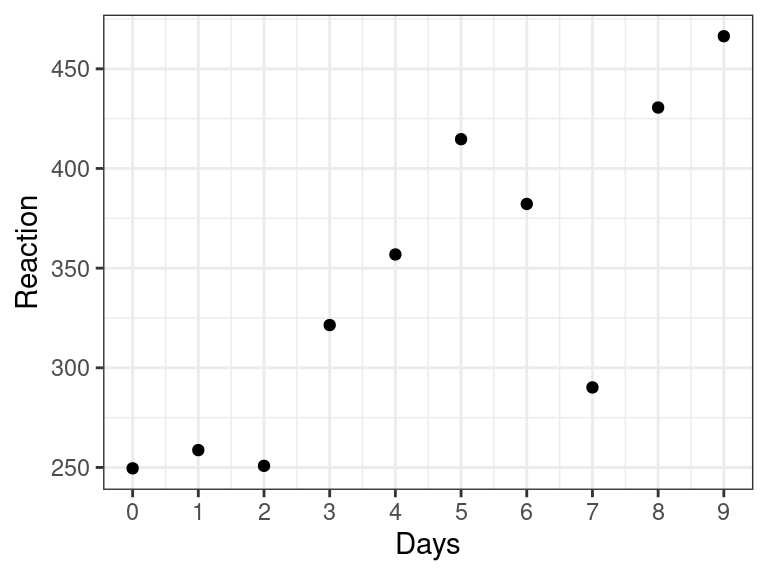
\includegraphics[width=0.5\linewidth]{05-linear-mixed-effects-intro_files/figure-latex/one-subject-1} 

}

\caption{*Data from a single subject in Belenky et al. (2003)*}\label{fig:one-subject}
\end{figure}

It looks like RT is increasing with each additional day of sleep deprivation, at least from day 2 to day 10.

\hypertarget{exercise}{%
\subsection*{Exercise}\label{exercise}}
\addcontentsline{toc}{subsection}{Exercise}

Use ggplot to recreate the plot below, which shows data for all 18 subjects.

\begin{figure}

{\centering 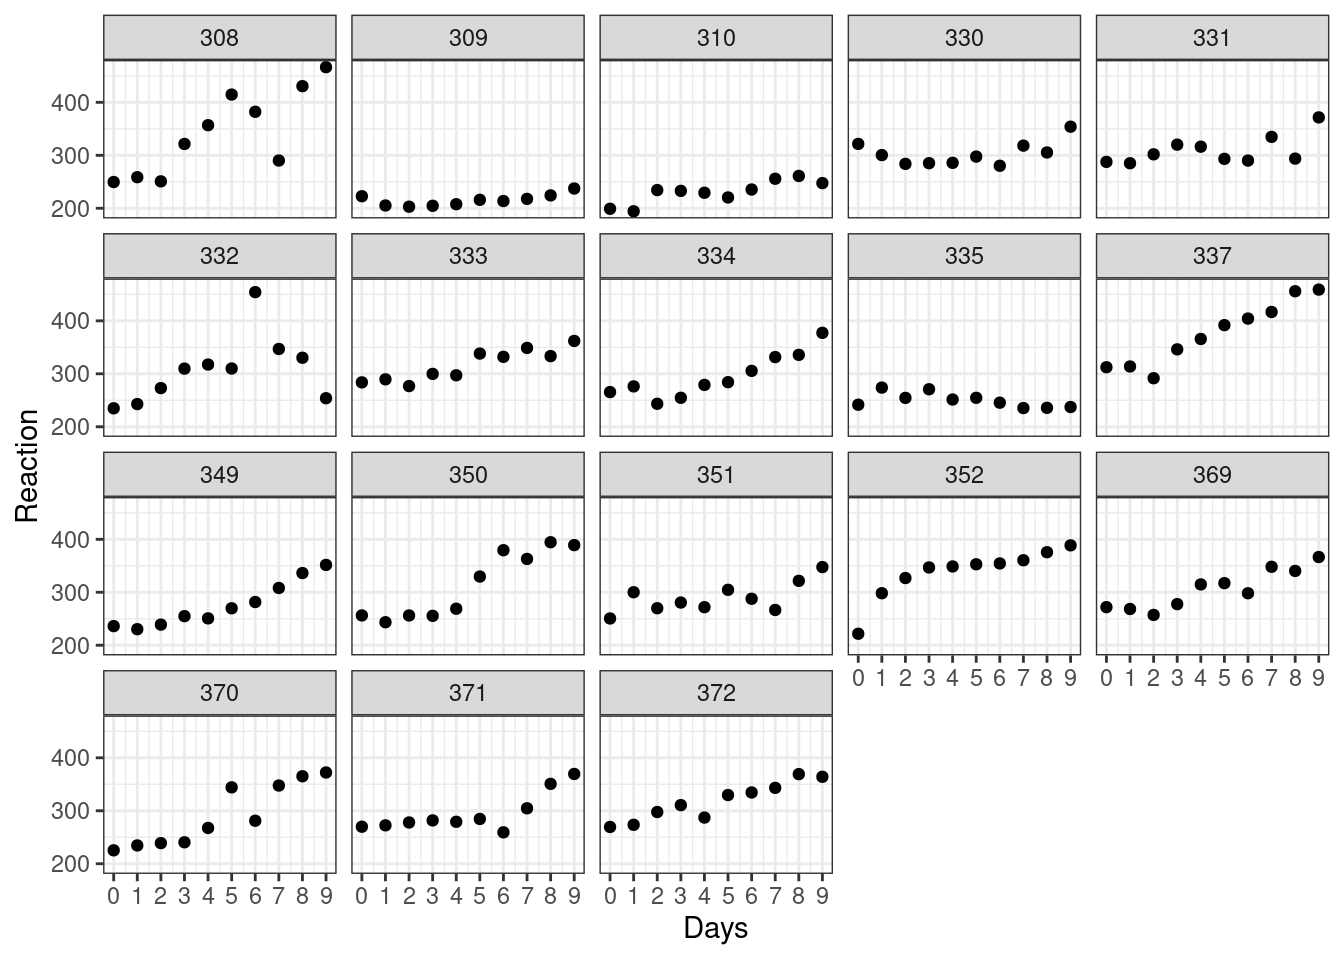
\includegraphics[width=1\linewidth]{05-linear-mixed-effects-intro_files/figure-latex/plot-solution0-1} 

}

\caption{*Data from Belenky et al. (2003)*}\label{fig:plot-solution0}
\end{figure}

Hint, please

Just above, you were given the code to make a plot for a single participant. Adapt this code to show all of the participants by getting rid of the \texttt{filter()} statement and adding a \emph{\texttt{ggplot2}} function that starts with \texttt{facet\_}.

Show me

Same as above, except you just add one line: \texttt{facet\_wrap(\textasciitilde{}Subject)}

\begin{Shaded}
\begin{Highlighting}[]
\KeywordTok{ggplot}\NormalTok{(sleepstudy, }\KeywordTok{aes}\NormalTok{(}\DataTypeTok{x =}\NormalTok{ Days, }\DataTypeTok{y =}\NormalTok{ Reaction)) }\OperatorTok{+}
\StringTok{  }\KeywordTok{geom_point}\NormalTok{() }\OperatorTok{+}
\StringTok{  }\KeywordTok{scale_x_continuous}\NormalTok{(}\DataTypeTok{breaks =} \DecValTok{0}\OperatorTok{:}\DecValTok{9}\NormalTok{) }\OperatorTok{+}
\StringTok{  }\KeywordTok{facet_wrap}\NormalTok{(}\OperatorTok{~}\NormalTok{Subject)}
\end{Highlighting}
\end{Shaded}

\hypertarget{how-to-model-this-data}{%
\section{How to model this data?}\label{how-to-model-this-data}}

Before proceeding, there is one important thing to note. Unfortunately, the description of the \texttt{sleepstudy} data in the \texttt{lme4} package is inaccurate. The documentation states:

\begin{quote}
On day 0 the subjects had their normal amount of sleep. Starting that night they were restricted to 3 hours of sleep per night.
\end{quote}

However, this is what \citet{Belenky_et_al_2003} actually say (p.~2 of the PDF):

\begin{quote}
The first 3 days (T1, T2 and B) were adaptation and training (T1 and T2) and baseline (B) and subjects were required to be in bed from 23:00 to 07:00 h {[}8 h required time in bed (TIB){]}. On the third day (B), baseline measures were taken. Beginning on the fourth day and continuing for a total of 7 days (E1--E7) subjects were in one of four sleep conditions {[}9 h required TIB (22:00--07:00 h), 7 h required TIB (24:00--07:00 h), 5 h required TIB (02:00--07:00 h), or 3 h required TIB (04:00--07:00 h){]}, effectively one sleep augmentation condition, and three sleep restriction conditions.
\end{quote}

One thing to note is that the dataset includes data from only one of the three conditions (the 3h TIB condition). But the more important thing is that the documentation of \texttt{sleepstudy} is wrong: there were seven nights of sleep restriction, not nine, with the first night of restriction occurring after the third day. The first two days, coded as \texttt{0}, \texttt{1}, were adaptation and training. The day coded as \texttt{2}, where the baseline measurement was taken should be the place where we start our analysis. If we include the days \texttt{0} and \texttt{1} in our analysis, this might bias our results, since any changes in performance during the first two days have to do with training, not sleep restriction.

\hypertarget{exercise-1}{%
\subsection*{Exercise}\label{exercise-1}}
\addcontentsline{toc}{subsection}{Exercise}

Remove from the dataset observations where \texttt{Days} is coded \texttt{0} or \texttt{1}, and then make a new variable \texttt{days\_deprived} from the \texttt{Days} variable so that the sequence starts at day 2, with day 2 being re-coded as day 0, day 3 as day 1, day 4 as day 2, etc. This new variable now tracks the number of days of sleep deprivation. Store the new table as \texttt{sleep2}.

Solution

\begin{Shaded}
\begin{Highlighting}[]
\NormalTok{sleep2 <-}\StringTok{ }\NormalTok{sleepstudy }\OperatorTok
\StringTok{  }\KeywordTok{filter}\NormalTok{(Days }\OperatorTok{>=}\StringTok{ }\NormalTok{2L) }\OperatorTok
\StringTok{  }\KeywordTok{mutate}\NormalTok{(}\DataTypeTok{days_deprived =}\NormalTok{ Days }\OperatorTok{-}\StringTok{ }\NormalTok{2L)}
\end{Highlighting}
\end{Shaded}

It is always a good idea to double check that the code works as intended. First, look at it:

\begin{Shaded}
\begin{Highlighting}[]
\KeywordTok{head}\NormalTok{(sleep2)}
\end{Highlighting}
\end{Shaded}

\begin{verbatim}
##   Reaction Days Subject days_deprived
## 1 250.8006    2     308             0
## 2 321.4398    3     308             1
## 3 356.8519    4     308             2
## 4 414.6901    5     308             3
## 5 382.2038    6     308             4
## 6 290.1486    7     308             5
\end{verbatim}

And check that \texttt{Days} and \texttt{days\_deprived} match up.

\begin{Shaded}
\begin{Highlighting}[]
\NormalTok{sleep2 }\OperatorTok
\StringTok{  }\KeywordTok{count}\NormalTok{(days_deprived, Days)}
\end{Highlighting}
\end{Shaded}

\begin{verbatim}
##   days_deprived Days  n
## 1             0    2 18
## 2             1    3 18
## 3             2    4 18
## 4             3    5 18
## 5             4    6 18
## 6             5    7 18
## 7             6    8 18
## 8             7    9 18
\end{verbatim}

Looks good. Note that the variable \texttt{n} in generated by \texttt{count()} and tells you how many rows there are for each unique combination of \texttt{Days} and \texttt{days\_deprived}. In this case, there were 18, one row for each participant.

Now let's re-plot the data looking at just these eight data points from Day 0 to Day 7. We've just copied the code from above, substituting \texttt{sleep2} for \texttt{sleepstudy} and using \texttt{days\_deprived} for our \texttt{x} variable.

\begin{Shaded}
\begin{Highlighting}[]
\KeywordTok{ggplot}\NormalTok{(sleep2, }\KeywordTok{aes}\NormalTok{(}\DataTypeTok{x =}\NormalTok{ days_deprived, }\DataTypeTok{y =}\NormalTok{ Reaction)) }\OperatorTok{+}
\StringTok{  }\KeywordTok{geom_point}\NormalTok{() }\OperatorTok{+}
\StringTok{  }\KeywordTok{scale_x_continuous}\NormalTok{(}\DataTypeTok{breaks =} \DecValTok{0}\OperatorTok{:}\DecValTok{7}\NormalTok{) }\OperatorTok{+}
\StringTok{  }\KeywordTok{facet_wrap}\NormalTok{(}\OperatorTok{~}\NormalTok{Subject) }\OperatorTok{+}
\StringTok{  }\KeywordTok{labs}\NormalTok{(}\DataTypeTok{y =} \StringTok{"Reaction Time"}\NormalTok{, }\DataTypeTok{x =} \StringTok{"Days deprived of sleep (0 = baseline)"}\NormalTok{)}
\end{Highlighting}
\end{Shaded}

\begin{figure}

{\centering 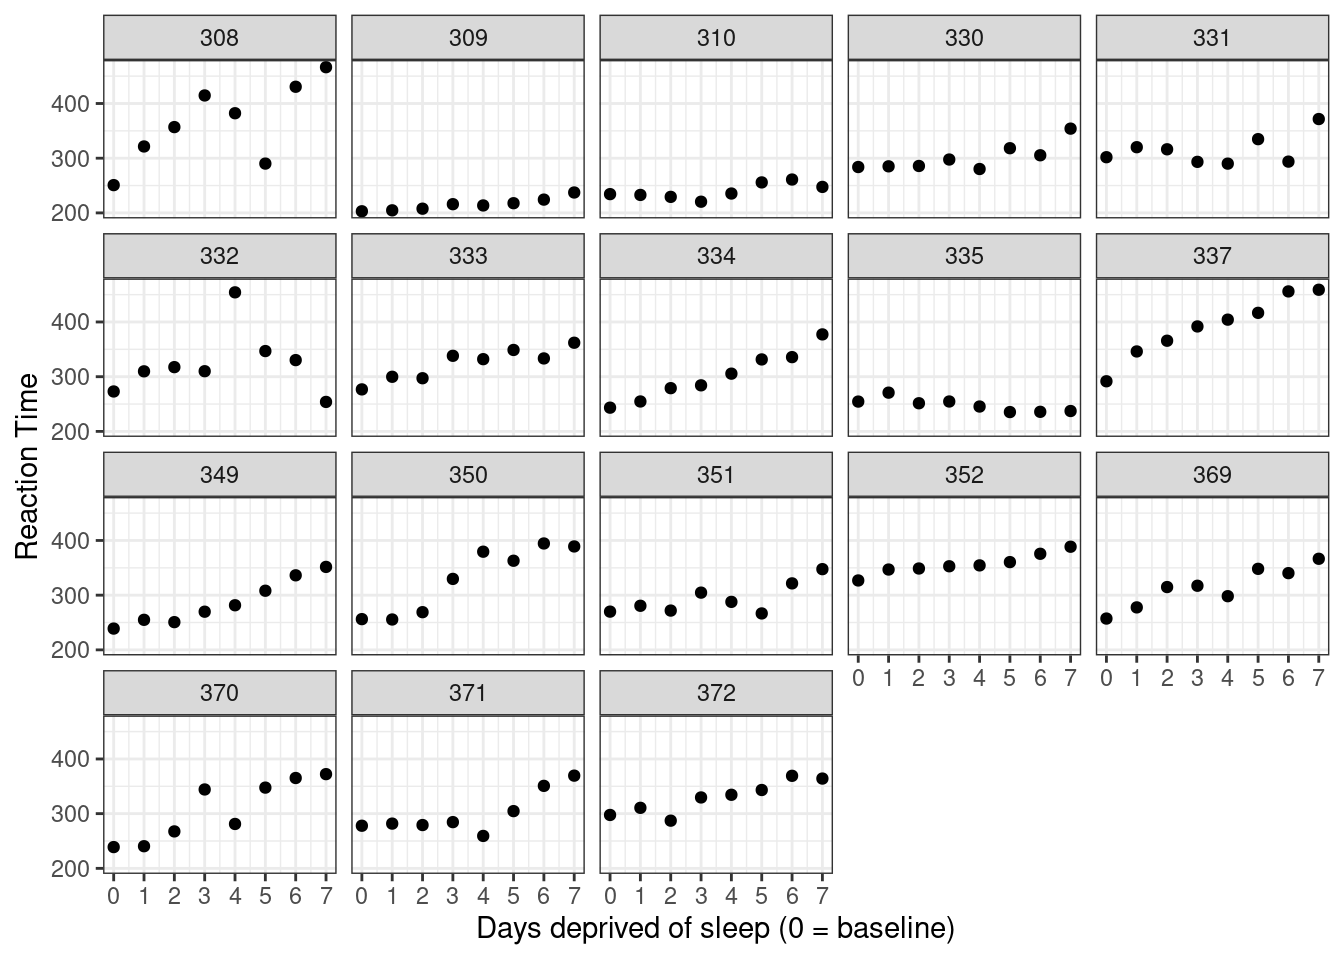
\includegraphics[width=1\linewidth]{05-linear-mixed-effects-intro_files/figure-latex/plot-solution2-1} 

}

\caption{*Data from Belenky et al. (2003), showing reaction time at baseline (0) and after each day of sleep deprivation.*}\label{fig:plot-solution2}
\end{figure}

Take a moment to think about how me might model the relationship between \texttt{days\_deprived} and \texttt{Reaction}. Does reaction time increase or decrease with increasing sleep deprivation? Is the relationship roughly stable or does it change with time?

With only one exception (subject 335) it looks like reaction time increases with each additional day of sleep deprivation. It looks like we could fit a line to each participant's data. Recall the general equation for a line is of the form \textbf{y = y-intercept + slope \(\times\) x}. In regression, the we usually express a linear relationship with the formula

\[Y = \beta_0 + \beta_1 X\]

where \(\beta_0\) is the y-intercept and \(\beta_1\) is the slope, parameters whose values we estimate from the data.

The lines will all differ in intercept (mean RT at day zero, before the sleep deprivation began) and slope (the change in RT with each additional day of sleep deprivation). But should we fit the same line to everyone? Or a totally different line for each subject? Or something somewhere in between?

Let's start by considering three different approaches we might take. Following McElreath, we will distinguish these approaches by calling them \textbf{complete pooling}, \textbf{no pooling}, and \textbf{partial pooling}.

\hypertarget{complete-pooling-one-size-fits-all}{%
\subsection{Complete pooling: One size fits all}\label{complete-pooling-one-size-fits-all}}

The \textbf{complete pooling} approach is a ``one-size-fits-all'' model: it estimates a single intercept and slope for the entire dataset, ignoring the fact that different subjects might vary in their intercepts or slopes. If that sounds like a bad approach, it is; but you know this because you've already visualized the data and noted that the pattern for each participant would seem to require different y-intercept and slope values.

Fitting one line is called the ``complete pooling'' approach because we pool together data from all subjects to get single estimates for an overall intercept and slope. The GLM for this approach is simply

\[Y_{sd} = \beta_0 + \beta_1 X_{sd} + e_{sd}\]

\[e_{sd} \sim N\left(0, \sigma^2\right)\]

where \(Y_{sd}\) is the mean RT for subject \(s\) on day \(d\), \(X_{sd}\) is the value of \texttt{Day} associated with that case (0-7), and \(e_{sd}\) is the error.

We would fit such a model in R using the \texttt{lm()} function, e.g.:

\begin{Shaded}
\begin{Highlighting}[]
\NormalTok{cp_model <-}\StringTok{ }\KeywordTok{lm}\NormalTok{(Reaction }\OperatorTok{~}\StringTok{ }\NormalTok{days_deprived, sleep2)}

\KeywordTok{summary}\NormalTok{(cp_model)}
\end{Highlighting}
\end{Shaded}

\begin{verbatim}
## 
## Call:
## lm(formula = Reaction ~ days_deprived, data = sleep2)
## 
## Residuals:
##      Min       1Q   Median       3Q      Max 
## -112.284  -26.732    2.143   27.734  140.453 
## 
## Coefficients:
##               Estimate Std. Error t value Pr(>|t|)    
## (Intercept)    267.967      7.737  34.633  < 2e-16 ***
## days_deprived   11.435      1.850   6.183 6.32e-09 ***
## ---
## Signif. codes:  0 '***' 0.001 '**' 0.01 '*' 0.05 '.' 0.1 ' ' 1
## 
## Residual standard error: 50.85 on 142 degrees of freedom
## Multiple R-squared:  0.2121,	Adjusted R-squared:  0.2066 
## F-statistic: 38.23 on 1 and 142 DF,  p-value: 6.316e-09
\end{verbatim}

According to this model, the predicted mean response time on Day 0 is about 268 milliseconds, with an increase of about 11 milliseconds per day of deprivation, on average. We can't trust the standard errors for our regression coefficients, however, because we are assuming that all of the observations are independent (technically, that the residuals are). However, we can be pretty sure this is a bad assumption.

Let's add the model predictions to the graph that we created above. We can use \texttt{geom\_abline()} to do so, specifying the intercept and slope for the line using the regression coefficients from the model fit, \texttt{coef(cp\_model)}, which returns a two-element vector with intercept and slope, respectively.

\begin{Shaded}
\begin{Highlighting}[]
\KeywordTok{coef}\NormalTok{(cp_model)}
\end{Highlighting}
\end{Shaded}

\begin{verbatim}
##   (Intercept) days_deprived 
##     267.96742      11.43543
\end{verbatim}

\begin{Shaded}
\begin{Highlighting}[]
\KeywordTok{ggplot}\NormalTok{(sleep2, }\KeywordTok{aes}\NormalTok{(}\DataTypeTok{x =}\NormalTok{ days_deprived, }\DataTypeTok{y =}\NormalTok{ Reaction)) }\OperatorTok{+}
\StringTok{  }\KeywordTok{geom_abline}\NormalTok{(}\DataTypeTok{intercept =} \KeywordTok{coef}\NormalTok{(cp_model)[}\DecValTok{1}\NormalTok{],}
              \DataTypeTok{slope =} \KeywordTok{coef}\NormalTok{(cp_model)[}\DecValTok{2}\NormalTok{],}
              \DataTypeTok{color =} \StringTok{'blue'}\NormalTok{) }\OperatorTok{+}
\StringTok{  }\KeywordTok{geom_point}\NormalTok{() }\OperatorTok{+}
\StringTok{  }\KeywordTok{scale_x_continuous}\NormalTok{(}\DataTypeTok{breaks =} \DecValTok{0}\OperatorTok{:}\DecValTok{7}\NormalTok{) }\OperatorTok{+}
\StringTok{  }\KeywordTok{facet_wrap}\NormalTok{(}\OperatorTok{~}\NormalTok{Subject) }\OperatorTok{+}
\StringTok{  }\KeywordTok{labs}\NormalTok{(}\DataTypeTok{y =} \StringTok{"Reaction Time"}\NormalTok{, }\DataTypeTok{x =} \StringTok{"Days deprived of sleep (0 = baseline)"}\NormalTok{)}
\end{Highlighting}
\end{Shaded}

\begin{figure}

{\centering 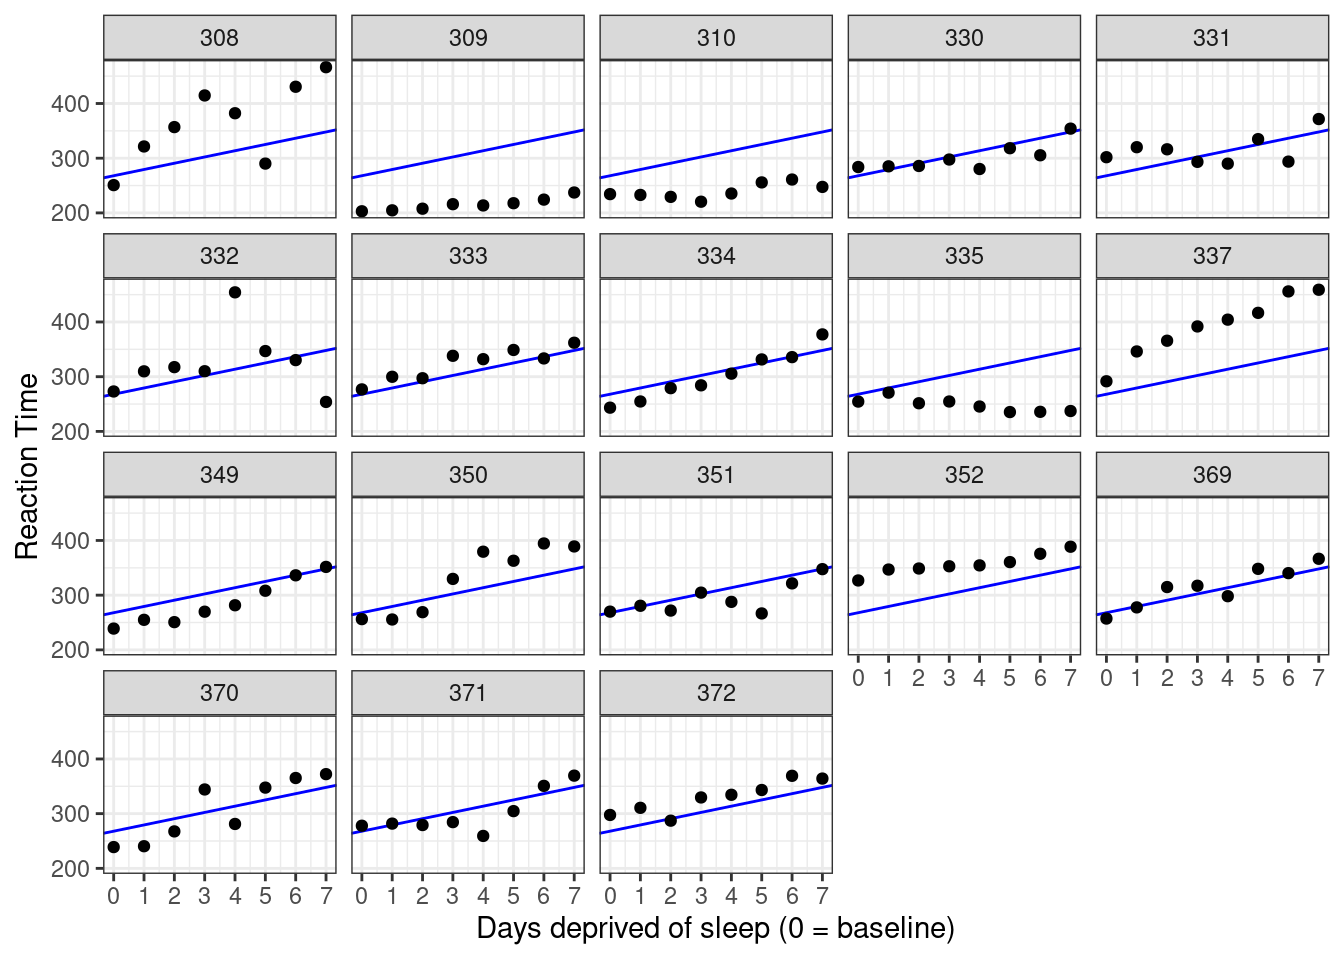
\includegraphics[width=1\linewidth]{05-linear-mixed-effects-intro_files/figure-latex/cp-model-plot-1} 

}

\caption{Data plotted against predictions from the complete pooling model.}\label{fig:cp-model-plot}
\end{figure}

The model fits the data badly. We need a different approach.

\hypertarget{no-pooling}{%
\subsection{No pooling}\label{no-pooling}}

Pooling all the information to get just one intercept and one slope estimate is inappropriate. Another approach would be to fit separate lines for each participant. This means that the estimates for each participant will be completely uninformed by the estimates for the other participants. In other words, we can separately estimate 18 individual intercept/slope pairs.

This model could be implemented in two ways: (1) by running separate regressions for each participant or (2) by running fixed-effects regression. We'll do the latter, so that everything is in one big model. We know how to do this already: we add in dummy codes for the \texttt{Subject} factor. We have 18 levels of this factor, so we'd need 17 dummy codes. Fortunately, R saves us from the trouble of creating the 17 variables we would need by hand. All we need to do is include \texttt{Subject} as a predictor in the model, and interact this categorical predictor with \texttt{days\_deprived} to allow intercepts and slopes to vary.

The variable \texttt{Subject} in the \texttt{sleep2} dataset is nominal. We just use numbers as labels to preserve anonymity, without intending to imply that Subject 310 is one point better than Subject 309 and two points better than 308. Make sure that you define it as a factor so that it is not included as a continuous variable!

We can test whether something is a factor in various ways. One is to use \texttt{summary()} on the table.

\begin{Shaded}
\begin{Highlighting}[]
\NormalTok{sleep2 }\OperatorTok\StringTok{ }\KeywordTok{summary}\NormalTok{()}
\end{Highlighting}
\end{Shaded}

\begin{verbatim}
##     Reaction          Days         Subject   days_deprived 
##  Min.   :203.0   Min.   :2.00   308    : 8   Min.   :0.00  
##  1st Qu.:265.2   1st Qu.:3.75   309    : 8   1st Qu.:1.75  
##  Median :303.2   Median :5.50   310    : 8   Median :3.50  
##  Mean   :308.0   Mean   :5.50   330    : 8   Mean   :3.50  
##  3rd Qu.:347.7   3rd Qu.:7.25   331    : 8   3rd Qu.:5.25  
##  Max.   :466.4   Max.   :9.00   332    : 8   Max.   :7.00  
##                                 (Other):96
\end{verbatim}

Here you can see that it is not treated as a number because rather than giving you distributional information (means, etc.) it tells you how many observations there are at each level.

You can also test it directly:

\begin{Shaded}
\begin{Highlighting}[]
\NormalTok{sleep2 }\OperatorTok\StringTok{ }\KeywordTok{pull}\NormalTok{(Subject) }\OperatorTok\StringTok{ }\KeywordTok{is.factor}\NormalTok{()}
\end{Highlighting}
\end{Shaded}

\begin{verbatim}
## [1] TRUE
\end{verbatim}

If something is not a factor, you can make it one be re-defining it using the \texttt{factor()} function.

\begin{Shaded}
\begin{Highlighting}[]
\NormalTok{np_model <-}\StringTok{ }\KeywordTok{lm}\NormalTok{(Reaction }\OperatorTok{~}\StringTok{ }\NormalTok{days_deprived }\OperatorTok{+}\StringTok{ }\NormalTok{Subject }\OperatorTok{+}\StringTok{ }\NormalTok{days_deprived}\OperatorTok{:}\NormalTok{Subject,}
               \DataTypeTok{data =}\NormalTok{ sleep2)}

\KeywordTok{summary}\NormalTok{(np_model)}
\end{Highlighting}
\end{Shaded}

\begin{verbatim}
## 
## Call:
## lm(formula = Reaction ~ days_deprived + Subject + days_deprived:Subject, 
##     data = sleep2)
## 
## Residuals:
##      Min       1Q   Median       3Q      Max 
## -106.521   -8.541    1.143    8.889  128.545 
## 
## Coefficients:
##                          Estimate Std. Error t value Pr(>|t|)    
## (Intercept)              288.2175    16.4772  17.492  < 2e-16 ***
## days_deprived             21.6905     3.9388   5.507 2.49e-07 ***
## Subject309               -87.9262    23.3023  -3.773 0.000264 ***
## Subject310               -62.2856    23.3023  -2.673 0.008685 ** 
## Subject330               -14.9533    23.3023  -0.642 0.522422    
## Subject331                 9.9658    23.3023   0.428 0.669740    
## Subject332                27.8157    23.3023   1.194 0.235215    
## Subject333                -2.7581    23.3023  -0.118 0.906000    
## Subject334               -50.2051    23.3023  -2.155 0.033422 *  
## Subject335               -25.3429    23.3023  -1.088 0.279207    
## Subject337                24.6143    23.3023   1.056 0.293187    
## Subject349               -59.2183    23.3023  -2.541 0.012464 *  
## Subject350               -40.2023    23.3023  -1.725 0.087343 .  
## Subject351               -24.2467    23.3023  -1.041 0.300419    
## Subject352                43.0655    23.3023   1.848 0.067321 .  
## Subject369               -21.5040    23.3023  -0.923 0.358154    
## Subject370               -53.3072    23.3023  -2.288 0.024107 *  
## Subject371               -30.4896    23.3023  -1.308 0.193504    
## Subject372                 2.4772    23.3023   0.106 0.915535    
## days_deprived:Subject309 -17.3334     5.5703  -3.112 0.002380 ** 
## days_deprived:Subject310 -17.7915     5.5703  -3.194 0.001839 ** 
## days_deprived:Subject330 -13.6849     5.5703  -2.457 0.015613 *  
## days_deprived:Subject331 -16.8231     5.5703  -3.020 0.003154 ** 
## days_deprived:Subject332 -19.2947     5.5703  -3.464 0.000765 ***
## days_deprived:Subject333 -10.8151     5.5703  -1.942 0.054796 .  
## days_deprived:Subject334  -3.5745     5.5703  -0.642 0.522423    
## days_deprived:Subject335 -25.8995     5.5703  -4.650 9.47e-06 ***
## days_deprived:Subject337   0.7518     5.5703   0.135 0.892895    
## days_deprived:Subject349  -5.2644     5.5703  -0.945 0.346731    
## days_deprived:Subject350   1.6007     5.5703   0.287 0.774382    
## days_deprived:Subject351 -13.1681     5.5703  -2.364 0.019867 *  
## days_deprived:Subject352 -14.4019     5.5703  -2.585 0.011057 *  
## days_deprived:Subject369  -7.8948     5.5703  -1.417 0.159273    
## days_deprived:Subject370  -1.0495     5.5703  -0.188 0.850912    
## days_deprived:Subject371  -9.3443     5.5703  -1.678 0.096334 .  
## days_deprived:Subject372 -10.6041     5.5703  -1.904 0.059613 .  
## ---
## Signif. codes:  0 '***' 0.001 '**' 0.01 '*' 0.05 '.' 0.1 ' ' 1
## 
## Residual standard error: 25.53 on 108 degrees of freedom
## Multiple R-squared:  0.849,	Adjusted R-squared:  0.8001 
## F-statistic: 17.35 on 35 and 108 DF,  p-value: < 2.2e-16
\end{verbatim}

What this model has done is take one subject to be the baseline (specifically, subject 308), and represent each subject in terms of offsets from that baseline. You saw this already when we talked about \href{05-interactions-course-notes.html\#cont-by-cat}{continuous-by-categorical interactions}.

Answer these questions (to three decimal places):

\begin{itemize}
\tightlist
\item
  What is the intercept for subject 308? 
\item
  What is the slope for subject 308? 
\item
  What is the intercept for subject 335? 
\item
  What is the slope for subject 335? 
\end{itemize}

Answers and Explanation

The baseline subject is 308; the default in R is to sort the levels of the factor alphabetically and chooses the first one as the baseline. This means that the intercept and slope for 308 are given by \texttt{(Intercept)} and \texttt{days\_deprived} respectively, because all of the other 17 dummy variables will be zero for subject 308.

All of the regression coefficients for the other subjects are represented as \emph{offsets} from this baseline subject. If we want to calculate the intercept and slope for a given subject, we just add in the corresponding offsets. So, the answers are

\begin{itemize}
\item
  intercept for 308: 288.217
\item
  slope for 308: 21.69
\item
  intercept for 335: \texttt{(Intercept)} + \texttt{Subject335} = 288.217 + -25.343 = 262.874
\item
  slope for 335: \texttt{days\_deprived} + \texttt{days\_deprived:Subject335} = 21.69 + -25.899 = -4.209
\end{itemize}

In the ``no pooling'' model, there is no \emph{overall} population intercept and slope that is being estimated; in this case, \texttt{(Intercept)} and \texttt{days\_deprived} are estimates of the intercept and slope for subject 308, which was (arbitrarily) chosen as the baseline subject. To get population estimates, we could introduce a second stage of analysis where we calculate means of the individual intercepts and slopes. Let's use the model estimates to calculate the intercepts and slopes for each subject.

\begin{Shaded}
\begin{Highlighting}[]
\NormalTok{all_intercepts <-}\StringTok{ }\KeywordTok{c}\NormalTok{(}\KeywordTok{coef}\NormalTok{(np_model)[}\StringTok{"(Intercept)"}\NormalTok{],}
                    \KeywordTok{coef}\NormalTok{(np_model)[}\DecValTok{3}\OperatorTok{:}\DecValTok{19}\NormalTok{] }\OperatorTok{+}\StringTok{ }\KeywordTok{coef}\NormalTok{(np_model)[}\StringTok{"(Intercept)"}\NormalTok{])}

\NormalTok{all_slopes  <-}\StringTok{ }\KeywordTok{c}\NormalTok{(}\KeywordTok{coef}\NormalTok{(np_model)[}\StringTok{"days_deprived"}\NormalTok{],}
                 \KeywordTok{coef}\NormalTok{(np_model)[}\DecValTok{20}\OperatorTok{:}\DecValTok{36}\NormalTok{] }\OperatorTok{+}\StringTok{ }\KeywordTok{coef}\NormalTok{(np_model)[}\StringTok{"days_deprived"}\NormalTok{])}

\NormalTok{ids <-}\StringTok{ }\NormalTok{sleep2 }\OperatorTok\StringTok{ }\KeywordTok{pull}\NormalTok{(Subject) }\OperatorTok\StringTok{ }\KeywordTok{levels}\NormalTok{() }\OperatorTok\StringTok{ }\KeywordTok{factor}\NormalTok{()}

\CommentTok{# make a tibble with the data extracted above}
\NormalTok{np_coef <-}\StringTok{ }\KeywordTok{tibble}\NormalTok{(}\DataTypeTok{Subject =}\NormalTok{ ids,}
                  \DataTypeTok{intercept =}\NormalTok{ all_intercepts,}
                  \DataTypeTok{slope =}\NormalTok{ all_slopes)}

\NormalTok{np_coef}
\end{Highlighting}
\end{Shaded}

\begin{verbatim}
## # A tibble: 18 x 3
##    Subject intercept slope
##    <fct>       <dbl> <dbl>
##  1 308          288. 21.7 
##  2 309          200.  4.36
##  3 310          226.  3.90
##  4 330          273.  8.01
##  5 331          298.  4.87
##  6 332          316.  2.40
##  7 333          285. 10.9 
##  8 334          238. 18.1 
##  9 335          263. -4.21
## 10 337          313. 22.4 
## 11 349          229. 16.4 
## 12 350          248. 23.3 
## 13 351          264.  8.52
## 14 352          331.  7.29
## 15 369          267. 13.8 
## 16 370          235. 20.6 
## 17 371          258. 12.3 
## 18 372          291. 11.1
\end{verbatim}

Let's see how well this model fits our data.

\begin{Shaded}
\begin{Highlighting}[]
\KeywordTok{ggplot}\NormalTok{(sleep2, }\KeywordTok{aes}\NormalTok{(}\DataTypeTok{x =}\NormalTok{ days_deprived, }\DataTypeTok{y =}\NormalTok{ Reaction)) }\OperatorTok{+}
\StringTok{  }\KeywordTok{geom_abline}\NormalTok{(}\DataTypeTok{data =}\NormalTok{ np_coef,}
              \DataTypeTok{mapping =} \KeywordTok{aes}\NormalTok{(}\DataTypeTok{intercept =}\NormalTok{ intercept,}
                            \DataTypeTok{slope =}\NormalTok{ slope),}
              \DataTypeTok{color =} \StringTok{'blue'}\NormalTok{) }\OperatorTok{+}
\StringTok{  }\KeywordTok{geom_point}\NormalTok{() }\OperatorTok{+}
\StringTok{  }\KeywordTok{scale_x_continuous}\NormalTok{(}\DataTypeTok{breaks =} \DecValTok{0}\OperatorTok{:}\DecValTok{7}\NormalTok{) }\OperatorTok{+}
\StringTok{  }\KeywordTok{facet_wrap}\NormalTok{(}\OperatorTok{~}\NormalTok{Subject) }\OperatorTok{+}
\StringTok{  }\KeywordTok{labs}\NormalTok{(}\DataTypeTok{y =} \StringTok{"Reaction Time"}\NormalTok{, }\DataTypeTok{x =} \StringTok{"Days deprived of sleep (0 = baseline)"}\NormalTok{)}
\end{Highlighting}
\end{Shaded}

\begin{figure}

{\centering 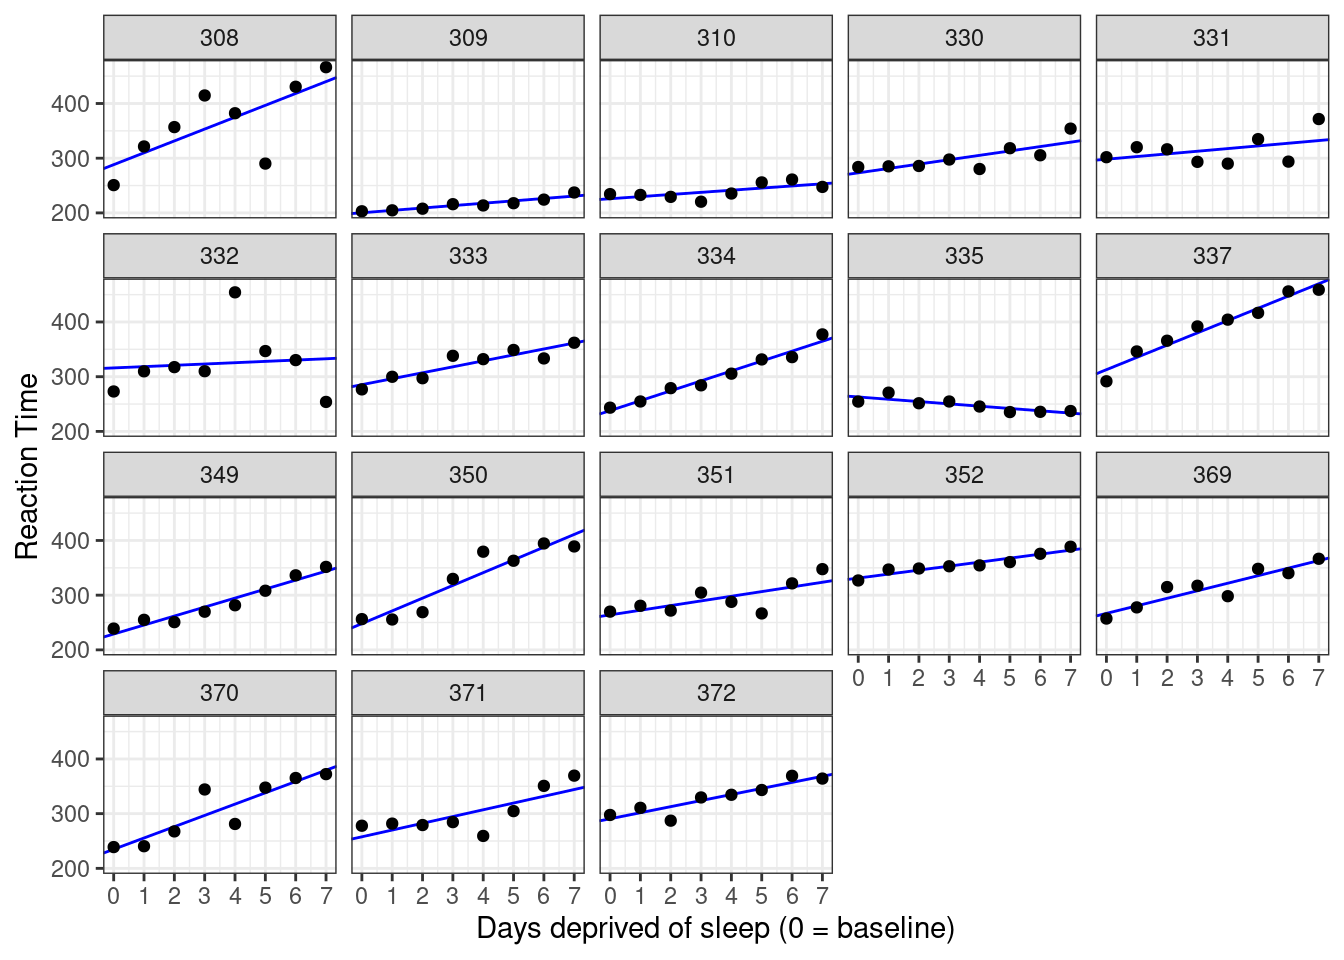
\includegraphics[width=1\linewidth]{05-linear-mixed-effects-intro_files/figure-latex/np-model-fits-1} 

}

\caption{Data plotted against fits from the no-pooling approach.}\label{fig:np-model-fits}
\end{figure}

This is much better than the complete pooling model. If we want to test the null hypothesis that the fixed slope is zero, we could do using a one-sample test.

\begin{Shaded}
\begin{Highlighting}[]
\NormalTok{np_coef }\OperatorTok\StringTok{ }\KeywordTok{pull}\NormalTok{(slope) }\OperatorTok\StringTok{ }\KeywordTok{t.test}\NormalTok{()}
\end{Highlighting}
\end{Shaded}

\begin{verbatim}
## 
## 	One Sample t-test
## 
## data:  .
## t = 6.1971, df = 17, p-value = 9.749e-06
## alternative hypothesis: true mean is not equal to 0
## 95 percent confidence interval:
##   7.542244 15.328613
## sample estimates:
## mean of x 
##  11.43543
\end{verbatim}

This tells us that the mean slope of
11.435
is significantly different from zero,
t(17) = 6.197, \(p < .001\).

\hypertarget{partial-pooling-using-mixed-effects-models}{%
\subsection{Partial pooling using mixed-effects models}\label{partial-pooling-using-mixed-effects-models}}

Neither the complete or no-pooling approach is satisfactory. It would be desirable to improve our estimates for individual participants by taking advantage of what we know about the other participants. This will help us better distinguish signal from error for each participant and improve generalization to the population. As the web app below will show, this becomes particularly important when we have unbalanced or missing data.

In the no-pooling model, we treated \texttt{Subject} as a \textbf{fixed factor}. Each pair of intercept and slope estimates is determined by that subject's data alone. However, we are not interested in these 18 subjects in and of themselves; rather, we are interested in them as examples drawn from a larger population of potential subjects. This subjects-as-fixed-effects approach is suboptimal if your goal is to generalize to new participants in the population of interest.

Partial pooling happens when you treat a factor as a random instead of fixed in your analysis. A \textbf{random factor} is a factor whose levels are considered to represent a proper subset of all the levels in the population. Usually, you treat a factor as random when the levels you have in the data are the result of sampling, and you want to generalize beyond those levels. In this case, we have eighteen unique subjects and thus, eighteen levels of the \texttt{Subject} factor, and would like to say something general about effects of sleep deprivation on the population of potential subjects.

Just as there are two types of factors---fixed and random---there are

A way to include random factors in your analysis is to use a linear mixed-effects model.

estimates at each level of the factor (i.e., for each subject) become informed by information from other levels (i.e., other subjects). Rather than estimating the intercept and slope for each participant without considering the estimates for other subjects, the model estimates values for the population, and pulls the estimates for individual subjects toward those values, a statistical phenomenon known as \texttt{shrinkage}.

The population estimates are informed by the individual estimates, but each individual estimate is ``pulled'' toward the population value.

The multilevel model is below. It is important that you understand the math and what it means. It looks complicated at first, but there's really nothing below that you haven't seen before. We'll explain everything step by step.

\emph{Level 1:}

\begin{equation}
Y_{sd} = \beta_{0s} + \beta_{1s} X_{sd} + e_{sd}
\end{equation}

\emph{Level 2:}

\begin{equation}
\beta_{0s} = \gamma_{0} + S_{0s}
\end{equation}

\begin{equation}
\beta_{1s} = \gamma_{1} + S_{1s}
\end{equation}

\emph{Variance Components:}

\begin{equation}
 \langle S_{0s}, S_{1s} \rangle \sim N\left(\langle 0, 0 \rangle, \mathbf{\Sigma}\right) 
\end{equation}

\begin{equation}
\mathbf{\Sigma} = \left(\begin{array}{cc}{\tau_{00}}^2 & \rho\tau_{00}\tau_{11} \\
         \rho\tau_{00}\tau_{11} & {\tau_{11}}^2 \\
         \end{array}\right) 
\end{equation}

\begin{equation}
e_{sd} \sim N\left(0, \sigma^2\right)
\end{equation}

In case you get lost, here's a table with an explanation for all of the variables in the set of equations above.

\begin{longtable}[]{@{}lll@{}}
\toprule
Variable & Type & Description\tabularnewline
\midrule
\endhead
\(Y_{sd}\) & observed & Value of \texttt{Reaction} for subject \(s\) on day \(d\)\tabularnewline
\(X_{sd}\) & observed & Value of \texttt{Day} (0-9) for subject \(s\) on day \(d\)\tabularnewline
\(\beta_{0s}\) & derived & level 1 intercept parameter\tabularnewline
\(\beta_{1s}\) & derived & level 1 slope parameter\tabularnewline
\(e_{sd}\) & derived & Residual (\(Y_{sd}\) - \(\hat{Y}_{sd}\)) for subject \(s\), day \(d\)\tabularnewline
\(\gamma_0\) & fixed & Grand intercept (``gamma'')\tabularnewline
\(\gamma_1\) & fixed & Grand slope (``gamma'')\tabularnewline
\(S_{0s}\) & derived & Random intercept (offset) for subject \(s\)\tabularnewline
\(S_{1s}\) & derived & Random slope (offset) for subject \(s\)\tabularnewline
\(\mathbf{\Sigma}\) & random & Variance-covariance matrix\tabularnewline
\({\tau_{00}}^2\) & random & Variance of random intercepts\tabularnewline
\(\rho\) & random & Random correlation between intercepts and slopes\tabularnewline
\({\tau_{11}}^2\) & random & Variance of random slopes\tabularnewline
\(\sigma^2\) & random & Error variance\tabularnewline
\bottomrule
\end{longtable}

Note the ``Status'' column of the table contains values \emph{fixed}, \emph{random}, and \emph{derived}. Although \emph{fixed} and \emph{random} are standard terms, \emph{derived} is not; I have introduced it to help you think about what these different variables mean in the context of the model and to help you distinguish variables that are directly estimated from variables that are not.

Let's begin with the Level 1 equation of our model, which represents the general relationship between the predictors and response variable. It captures the functional form of the main relationship between reaction time \(Y_{sd}\) and sleep deprivation \(X_{sd}\): a straight line with intercept \(\beta_{0s}\) and slope \(\beta_{1s}\). Now \(\beta_{0s}\) and \(\beta_{1s}\) makes it look like the complete pooling model, where we estimated a single intercept and single slope for the entire dataset; however, we're not actually estimating these directly. Instead, we're going to think of \(\beta_{0s}\) and \(\beta_{1s}\) as derived: they are wholly defined by variables at Level 2 of the model.

Level 2 of the model, defined by two equations, represents relationships at the participant level. Here, we define the intercept \(\beta_{0s}\) in terms of a fixed effect \(\gamma_0\) and a \emph{random intercept} \(S_{0s}\); likewise, we define the slope \(\beta_{1s}\) in terms of a fixed slope \(\gamma_1\) and a \emph{random slope} \(S_{1s}\).

The final equations represent the \emph{Variance Components} of the model. We'll get into this more in detail below.

Let's substitute the Level 2 equations into Level 1 to see the advantages of representing things in the multilevel way.

\begin{equation}
Y_{sd} = \gamma_{0} + S_{0s} + \left(\gamma_{1} + S_{1s}\right) X_{sd} + e_{sd}
\end{equation}

While this ``combined'' formula syntax is easy enough to understand in this particular case, the multilevel form more clearly allows us to see the functional form of the model: a straight line. We could easily change the functional form to, for instance, capture non-linear trends:

\[Y_{sd} = \beta_{0s} + \beta_{1s} X_{sd} + \beta_{2s} X_{sd}^2 + e_{sd}\]

This functional form gets obscured in the combined syntax. The multilevel syntax also makes it easy to see which terms go with the intercept and which terms go with the slope. Also, as designs get more compilicated---for example, if we were to assign participants to different experimental conditions, thus introducing a further predictors at Level 2---the combined equations get harder and harder to parse and reason about.

Fixed effect parameters like \(\gamma_0\) and \(\gamma_1\) are estimated from the data, and reflect stable properties of the population. In this example, \(\gamma_0\) is the population intercept and \(\gamma_1\) is the population slope. You can think of these \textbf{fixed-effects parameters} as representing the \textbf{average intercept and slope} in the population. These are ``fixed'' in the sense that we assume that they reflect the true underlying values in the population; they are not assumed to vary from sample to sample. These fixed effects parameters are often of prime theoretical interest; we want to measure them and their standard errors in a manner that is as unbiased and precise as the data allow. In experimental settings they are often the targets of hypothesis tests.

Random effects like \(S_{0i}\) and \(S_{1i}\) allow intercepts and slopes (respectively) to vary over subjects. These random effects are \emph{offsets}: deviations from the population `grand mean' values. Some subjects will just be slower responders than others, such that they will have a higher intercept (mean RT) on day 0 than the population's estimated value of \(\hat{\gamma_0}\). These slower-than-average subjects will have positive \(S_{0i}\) values; faster-than-average subjects will have negative \(S_{0i}\) values. Likewise, some subjects will show stronger effects of sleep deprivation (steeper slope) than the estimated population effect, \(\hat{\gamma_1}\), which implies a positive offset \(S_{1s}\), while others may show weaker effects or close to none at all (negative offset).

Each participant can be represented as a vector pair \(\langle S_{0i}, S_{1i} \rangle\). If the subjects in our sample comprised the entire population, we would be justified in treating them as fixed and estimating their values, as in the ``no-pooling'' approach above. This is not the case here. In recognition of the fact they are sampled, we are going to treat subjects as a random factor rather than a fixed factor. Instead of estimate the values for the subjects we happened to pick, we will estimate \textbf{the covariance matrix that represents the bivariate distribution from which these pairs of values are drawn}. By doing this, we allow the subjects in the sample to inform us about characteristics of the population.

\hypertarget{the-variance-covariance-matrix}{%
\subsection{The variance-covariance matrix}\label{the-variance-covariance-matrix}}

\begin{equation}
 \langle S_{0s}, S_{1s} \rangle \sim N\left(\langle 0, 0 \rangle, \mathbf{\Sigma}\right) 
\end{equation}

\begin{equation}
\mathbf{\Sigma} = \left(\begin{array}{cc}{\tau_{00}}^2 & \rho\tau_{00}\tau_{11} \\
         \rho\tau_{00}\tau_{11} & {\tau_{11}}^2 \\
         \end{array}\right) 
\end{equation}

Equations in the \emph{Variance Components} characterize our estimates of variability. The first equation states our assumption that the random intercept / random slope pairs \(\langle S_{0s}, S_{1s} \rangle\) are drawn from a bivariate normal distribution centered at the origin \(\langle 0, 0 \rangle\) with variance-covariance matrix \(\mathbf{\Sigma}\).

The variance-covariance matrix is key: it determines the probability of drawing random effect pairs \(\langle S_{0s}, S_{1s} \rangle\) from the population. You have seen these before, in the \href{03-bivariate-simulation.html}{chapter on correlation and regression}. The covariance matrix is always a square matrix (equal numbers of columns and rows). On the main diagonal (upper left and bottom right cells) it has random effect variances \({\tau_{00}}^2\) and \({\tau_{11}}^2\). \({\tau_{00}}^2\) is the random intercept variance, which captures how much subjects vary in their mean response time on Day 0, before any sleep deprivation. \({\tau_{11}}^2\) is the random slope variance, which captures how much subjects vary in their susceptibility to the effects of sleep deprivation.

The cells in the off-diagonal contain covariances, but this information is represented redundantly in the matrix; the lower left element is identical to the upper right element; both capture the covariance between random intercepts and slopes, as expressed by \(\rho\tau_{00}\tau_{11}\). In this equation \(\rho\) is the correlation between the intercept and slope. So, all the information in the matrix can be captured by just three parameters: \(\tau_{00}\), \(\tau_{11}\), and \(\rho\).

\hypertarget{estimating-the-model-parameters}{%
\section{Estimating the model parameters}\label{estimating-the-model-parameters}}

To estimate parameters, we are going to use the \texttt{lmer()} function of the lme4 package (Bates, Mächler, Bolker, \& Walker, 2015). The basic syntax of \texttt{lmer()} is

\begin{verbatim}
lmer(formula, data, ...)
\end{verbatim}

where \texttt{formula} expresses the structure of the underlying model in a compact format and \texttt{data} is the data frame where the variables mentioned in the formula can be found.

The general format of the model formula for N fixed effects (\texttt{fix}) and K random effects (\texttt{ran}) is

\texttt{DV\ \textasciitilde{}\ fix1\ +\ fix2\ +\ ...\ +\ fixN\ +\ (ran1\ +\ ran2\ +\ ...\ +\ ranK\ \textbar{}\ random\_factor1)}

Interactions between factors A and B can be specified using either \texttt{A\ *\ B} (interaction and main effects) or \texttt{A:B} (just the interaction).

A key difference from standard R model syntax is the presence of a random effect term, which is enclosed in parentheses, e.g., \texttt{(ran1\ +\ ran2\ +\ ...\ +\ ranK\ \textbar{}\ random\_factor)}. Each bracketed expression represents random effects associated with a single random factor. You can have more than one random effects term in a single formula, as we will see when we talk about crossed random factors. You should think of the random effects terms as providing \texttt{lmer()} with \textbf{instructions on how to construct variance-covariance matrices}.

On the left side of the bar \texttt{\textbar{}} you put the effects you want to allow to vary over the levels of the random factor named on the right side. Usually, the right-side variable is one whose values uniquely identify individual subjects (e.g., \texttt{subject\_id}).

Consider the following possible model formulas for the \texttt{sleep2} data and the variance-covariance matrices they construct.

\begin{longtable}[]{@{}lll@{}}
\toprule
\begin{minipage}[b]{0.04\columnwidth}\raggedright
\strut
\end{minipage} & \begin{minipage}[b]{0.35\columnwidth}\raggedright
model\strut
\end{minipage} & \begin{minipage}[b]{0.53\columnwidth}\raggedright
syntax\strut
\end{minipage}\tabularnewline
\midrule
\endhead
\begin{minipage}[t]{0.04\columnwidth}\raggedright
1\strut
\end{minipage} & \begin{minipage}[t]{0.35\columnwidth}\raggedright
random intercepts only\strut
\end{minipage} & \begin{minipage}[t]{0.53\columnwidth}\raggedright
\texttt{Reaction\ \textasciitilde{}\ days\_deprived\ +\ (1\ \textbar{}\ Subject)}\strut
\end{minipage}\tabularnewline
\begin{minipage}[t]{0.04\columnwidth}\raggedright
2\strut
\end{minipage} & \begin{minipage}[t]{0.35\columnwidth}\raggedright
random intercepts and slopes\strut
\end{minipage} & \begin{minipage}[t]{0.53\columnwidth}\raggedright
\texttt{Reaction\ \textasciitilde{}\ days\_deprived\ +\ (1\ +\ days\_deprived\ \textbar{}\ Subject)}\strut
\end{minipage}\tabularnewline
\begin{minipage}[t]{0.04\columnwidth}\raggedright
3\strut
\end{minipage} & \begin{minipage}[t]{0.35\columnwidth}\raggedright
model 2 alternate syntax\strut
\end{minipage} & \begin{minipage}[t]{0.53\columnwidth}\raggedright
\texttt{Reaction\ \textasciitilde{}\ days\_deprived\ +\ (days\_deprived\ \textbar{}\ Subject)}\strut
\end{minipage}\tabularnewline
\begin{minipage}[t]{0.04\columnwidth}\raggedright
4\strut
\end{minipage} & \begin{minipage}[t]{0.35\columnwidth}\raggedright
random slopes only\strut
\end{minipage} & \begin{minipage}[t]{0.53\columnwidth}\raggedright
\texttt{Reaction\ \textasciitilde{}\ days\_deprived\ +\ (0\ +\ days\_deprived\ \textbar{}\ Subject)}\strut
\end{minipage}\tabularnewline
\begin{minipage}[t]{0.04\columnwidth}\raggedright
5\strut
\end{minipage} & \begin{minipage}[t]{0.35\columnwidth}\raggedright
model 2 + zero-covariances\strut
\end{minipage} & \begin{minipage}[t]{0.53\columnwidth}\raggedright
\texttt{Reaction\ \textasciitilde{}\ days\_deprived\ +\ (days\_deprived\ \textbar{}\textbar{}\ Subject)}\strut
\end{minipage}\tabularnewline
\bottomrule
\end{longtable}

\emph{Model 1:}

\begin{equation*}
  \mathbf{\Sigma} = \left(
  \begin{array}{cc}
    {\tau_{00}}^2 & 0 \\
                0 & 0 \\
  \end{array}\right) 
\end{equation*}

\emph{Models 2 and 3:}

\begin{equation*}
  \mathbf{\Sigma} = \left(
  \begin{array}{cc}
             {\tau_{00}}^2 & \rho\tau_{00}\tau_{11} \\
    \rho\tau_{00}\tau_{11} &          {\tau_{11}}^2 \\
  \end{array}\right) 
\end{equation*}

\emph{Model 4:}

\begin{equation*}
  \mathbf{\Sigma} = \left(
  \begin{array}{cc}
    0 &             0 \\
    0 & {\tau_{11}}^2 \\
  \end{array}\right) 
\end{equation*}

\emph{Model 5:}

\begin{equation*}
  \mathbf{\Sigma} = \left(
  \begin{array}{cc}
    {\tau_{00}}^2 &             0 \\
                0 & {\tau_{11}}^2 \\
  \end{array}\right) 
\end{equation*}

The most reasonable model for these data is Model 2, so we'll stick with that.

Let's fit the model, storing the result in object \texttt{pp\_mod}.

\begin{Shaded}
\begin{Highlighting}[]
\NormalTok{pp_mod <-}\StringTok{ }\KeywordTok{lmer}\NormalTok{(Reaction }\OperatorTok{~}\StringTok{ }\NormalTok{days_deprived }\OperatorTok{+}\StringTok{ }\NormalTok{(days_deprived }\OperatorTok{|}\StringTok{ }\NormalTok{Subject), sleep2)}

\KeywordTok{summary}\NormalTok{(pp_mod)}
\end{Highlighting}
\end{Shaded}

\begin{verbatim}
## Linear mixed model fit by REML ['lmerMod']
## Formula: Reaction ~ days_deprived + (days_deprived | Subject)
##    Data: sleep2
## 
## REML criterion at convergence: 1404.1
## 
## Scaled residuals: 
##     Min      1Q  Median      3Q     Max 
## -4.0157 -0.3541  0.0069  0.4681  5.0732 
## 
## Random effects:
##  Groups   Name          Variance Std.Dev. Corr
##  Subject  (Intercept)   958.35   30.957       
##           days_deprived  45.78    6.766   0.18
##  Residual               651.60   25.526       
## Number of obs: 144, groups:  Subject, 18
## 
## Fixed effects:
##               Estimate Std. Error t value
## (Intercept)    267.967      8.266  32.418
## days_deprived   11.435      1.845   6.197
## 
## Correlation of Fixed Effects:
##             (Intr)
## days_deprvd -0.062
\end{verbatim}

Before discussing how to interpret the output, let's first plot the data against our model predictions. We can get model predictions using the \texttt{predict()} function (see \texttt{?predict.merMod} for information about use with mixed-effects models).

First, create a new data frame with predictor values for \texttt{Subject} and \texttt{days\_deprived}.

\begin{Shaded}
\begin{Highlighting}[]
\NormalTok{newdata <-}\StringTok{ }\KeywordTok{crossing}\NormalTok{(}
  \DataTypeTok{Subject =}\NormalTok{ sleep2 }\OperatorTok\StringTok{ }\KeywordTok{pull}\NormalTok{(Subject) }\OperatorTok\StringTok{ }\KeywordTok{levels}\NormalTok{() }\OperatorTok\StringTok{ }\KeywordTok{factor}\NormalTok{(),}
  \DataTypeTok{days_deprived =} \DecValTok{0}\OperatorTok{:}\DecValTok{7}\NormalTok{)}

\NormalTok{newdata}
\end{Highlighting}
\end{Shaded}

\begin{verbatim}
## # A tibble: 144 x 2
##    Subject days_deprived
##    <fct>           <int>
##  1 308                 0
##  2 308                 1
##  3 308                 2
##  4 308                 3
##  5 308                 4
##  6 308                 5
##  7 308                 6
##  8 308                 7
##  9 309                 0
## 10 309                 1
## # ... with 134 more rows
\end{verbatim}

Then, run this through \texttt{predict()}. Typically we will add the prediction in as a new variable in the data frame of new data, giving it the same name as our DV (\texttt{Reaction}).

\begin{Shaded}
\begin{Highlighting}[]
\NormalTok{newdata2 <-}\StringTok{ }\NormalTok{newdata }\OperatorTok
\StringTok{  }\KeywordTok{mutate}\NormalTok{(}\DataTypeTok{Reaction =} \KeywordTok{predict}\NormalTok{(pp_mod, newdata))}
\end{Highlighting}
\end{Shaded}

Now we are ready to plot.

\begin{Shaded}
\begin{Highlighting}[]
\KeywordTok{ggplot}\NormalTok{(sleep2, }\KeywordTok{aes}\NormalTok{(}\DataTypeTok{x =}\NormalTok{ days_deprived, }\DataTypeTok{y =}\NormalTok{ Reaction)) }\OperatorTok{+}
\StringTok{  }\KeywordTok{geom_line}\NormalTok{(}\DataTypeTok{data =}\NormalTok{ newdata2,}
            \DataTypeTok{color =} \StringTok{'blue'}\NormalTok{) }\OperatorTok{+}
\StringTok{  }\KeywordTok{geom_point}\NormalTok{() }\OperatorTok{+}
\StringTok{  }\KeywordTok{scale_x_continuous}\NormalTok{(}\DataTypeTok{breaks =} \DecValTok{0}\OperatorTok{:}\DecValTok{7}\NormalTok{) }\OperatorTok{+}
\StringTok{  }\KeywordTok{facet_wrap}\NormalTok{(}\OperatorTok{~}\NormalTok{Subject) }\OperatorTok{+}
\StringTok{  }\KeywordTok{labs}\NormalTok{(}\DataTypeTok{y =} \StringTok{"Reaction Time"}\NormalTok{, }\DataTypeTok{x =} \StringTok{"Days deprived of sleep (0 = baseline)"}\NormalTok{)}
\end{Highlighting}
\end{Shaded}

\begin{figure}

{\centering 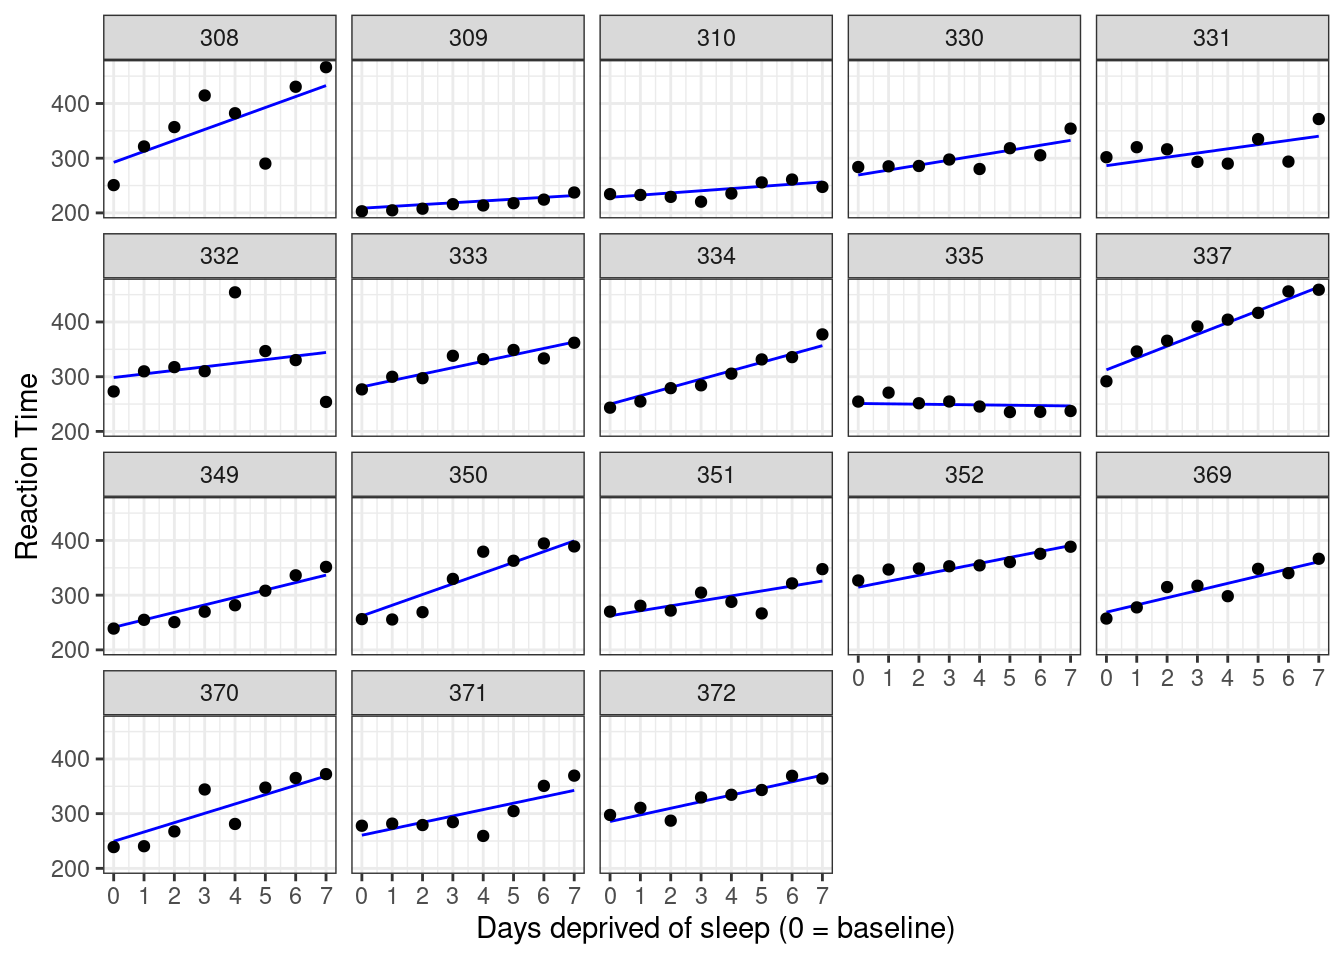
\includegraphics[width=1\linewidth]{05-linear-mixed-effects-intro_files/figure-latex/pp-plot-1} 

}

\caption{Data plotted against predictions from a partial pooling approach.}\label{fig:pp-plot}
\end{figure}

\hypertarget{interpreting-lmer-output-and-extracting-estimates}{%
\section{\texorpdfstring{Interpreting \texttt{lmer()} output and extracting estimates}{Interpreting lmer() output and extracting estimates}}\label{interpreting-lmer-output-and-extracting-estimates}}

The call to \texttt{lmer()} returns a fitted model object of class ``lmerMod''. To find out more about the \texttt{lmerMod} class, which is in turn a specialized version of the \texttt{merMod} class, see \texttt{?lmerMod-class}.

\hypertarget{fixed-effects}{%
\subsection{Fixed effects}\label{fixed-effects}}

The section of the output called \texttt{Fixed\ effects:} should look familiar; it is similar to what you would see in the output for a simple linear model fit by \texttt{lm()}.

\begin{verbatim}
## Fixed effects:
##               Estimate Std. Error t value
## (Intercept)    267.967      8.266  32.418
## days_deprived   11.435      1.845   6.197
\end{verbatim}

This indicates that the estimated mean reaction time for participants at Day 0 was about
268 milliseconds,
with each day of sleep deprivation adding an additional
11 milliseconds
to the response time, on average.

If we need to get the fixed effects from the model, we can extract them using \texttt{fixef()}.

\begin{Shaded}
\begin{Highlighting}[]
\KeywordTok{fixef}\NormalTok{(pp_mod)}
\end{Highlighting}
\end{Shaded}

\begin{verbatim}
##   (Intercept) days_deprived 
##     267.96742      11.43543
\end{verbatim}

The standard errors give us estimates of the variability for these parameters due to sampling error. You could use these to calculate the \(t\)-values or derive confidence intervals. Extract them using \texttt{vcov(pp\_mod)} which gives a variance-covariance matrix (\emph{not} the one associated with the random effects), pull out the diagonal using \texttt{diag()} and then take the square root using \texttt{sqrt()}.

\begin{Shaded}
\begin{Highlighting}[]
\KeywordTok{sqrt}\NormalTok{(}\KeywordTok{diag}\NormalTok{(}\KeywordTok{vcov}\NormalTok{(pp_mod)))}

\CommentTok{# OR, equivalently using pipes:}
\CommentTok{# vcov(pp_mod) %>% diag() %>% sqrt()}
\end{Highlighting}
\end{Shaded}

\begin{verbatim}
## [1] 8.265896 1.845293
\end{verbatim}

Note that these \(t\) values do not appear with \(p\) values, as is customary in simpler modeling frameworks. There are multiple approaches for getting \(p\) values from mixed-effects models, with advantages and disadvantages to each; see \citet{Luke_2017} for a survey of options. The \(t\) values do not appear with degrees of freedom, because the degrees of freedom in a mixed-effects model are not well-defined. Often people will treat them as Wald \(z\) values, i.e., as observations from the standard normal distribution. Because the \(t\) distribution asymptotes the standard normal distribution as the number of observations goes to infinity, this ``t-as-z'' practice is legitimate if you have a large enough set of observations.

To calculate the Wald \(z\) values, just divide the fixed effect estimate by its standard error:

\begin{Shaded}
\begin{Highlighting}[]
\NormalTok{tvals <-}\StringTok{ }\KeywordTok{fixef}\NormalTok{(pp_mod) }\OperatorTok{/}\StringTok{ }\KeywordTok{sqrt}\NormalTok{(}\KeywordTok{diag}\NormalTok{(}\KeywordTok{vcov}\NormalTok{(pp_mod)))}

\NormalTok{tvals}
\end{Highlighting}
\end{Shaded}

\begin{verbatim}
##   (Intercept) days_deprived 
##     32.418437      6.197082
\end{verbatim}

You can get the associated \(p\)-values using the following formula:

\begin{Shaded}
\begin{Highlighting}[]
\DecValTok{2} \OperatorTok{*}\StringTok{ }\NormalTok{(}\DecValTok{1} \OperatorTok{-}\StringTok{ }\KeywordTok{pnorm}\NormalTok{(}\KeywordTok{abs}\NormalTok{(tvals)))}
\end{Highlighting}
\end{Shaded}

\begin{verbatim}
##   (Intercept) days_deprived 
##   0.00000e+00   5.75197e-10
\end{verbatim}

This gives us strong evidence against the null hypothesis \(H_0: \gamma_1 = 0\). Sleep deprivation does appear to increase response time.

You can get confidence intervals for the estimates using \texttt{confint()} (this technique uses the \emph{parametric bootstrap}). \texttt{confint()} is a generic function, so to get help on this function, use \texttt{?confint.merMod}.

\begin{Shaded}
\begin{Highlighting}[]
\KeywordTok{confint}\NormalTok{(pp_mod)}
\end{Highlighting}
\end{Shaded}

\begin{verbatim}
## Computing profile confidence intervals ...
\end{verbatim}

\begin{verbatim}
##                     2.5 %      97.5 %
## .sig01         19.0979934  46.3366599
## .sig02         -0.4051073   0.8058951
## .sig03          4.0079284  10.2487351
## .sigma         22.4666029  29.3494509
## (Intercept)   251.3443396 284.5904989
## days_deprived   7.7245247  15.1463328
\end{verbatim}

\hypertarget{random-effects}{%
\subsection{Random effects}\label{random-effects}}

\begin{verbatim}
## Random effects:
##  Groups   Name          Variance Std.Dev. Corr
##  Subject  (Intercept)   958.35   30.957       
##           days_deprived  45.78    6.766   0.18
##  Residual               651.60   25.526       
## Number of obs: 144, groups:  Subject, 18
\end{verbatim}

The random effects part of the \texttt{summary()} output is less familiar. What you find here is a table with information about the variance components: the variance-covariance matrix (or matrices, if you have multiple random factors) and the residual variance.

Let's start with the \texttt{Residual} line. This tells us that the residual variance, \(\sigma^2\), was estimated at about
651.6. The value in the next column,
25.526, is just the standard deviation, \(\sigma\), which is the square root of the variance.

We extract the residual standard deviation using the \texttt{sigma()} function.

\begin{Shaded}
\begin{Highlighting}[]
\KeywordTok{sigma}\NormalTok{(pp_mod) }\CommentTok{# residual}
\end{Highlighting}
\end{Shaded}

\begin{verbatim}
## [1] 25.5264
\end{verbatim}

The two lines above the \texttt{Residual} line give us information about the variance-covariance matrix for the \texttt{Subject} random factor.

\begin{verbatim}
##  Groups   Name          Variance Std.Dev. Corr
##  Subject  (Intercept)   958.35   30.957       
##           days_deprived  45.78    6.766   0.18
\end{verbatim}

The values in the \texttt{Variance} column gives us the main diagonal of the matrix, and the \texttt{Std.Dev.} values are just the square roots of these values. The \texttt{Corr} column tells us the correlation between the intercept and slope.

We can extract these values from the fitted object \texttt{pp\_mod} using the \texttt{VarCorr()} function. This returns a named list, with one element for each random factor. We have \texttt{Subject} as our only random factor, so the list will just be of length 1.

\begin{Shaded}
\begin{Highlighting}[]
\CommentTok{# variance-covariance matrix for random factor Subject}
\KeywordTok{VarCorr}\NormalTok{(pp_mod)[[}\StringTok{"Subject"}\NormalTok{]] }\CommentTok{# equivalently: VarCorr(pp_mod)[[1]]}
\end{Highlighting}
\end{Shaded}

\begin{verbatim}
##               (Intercept) days_deprived
## (Intercept)      958.3517      37.20460
## days_deprived     37.2046      45.77766
## attr(,"stddev")
##   (Intercept) days_deprived 
##     30.957255      6.765919 
## attr(,"correlation")
##               (Intercept) days_deprived
## (Intercept)     1.0000000     0.1776263
## days_deprived   0.1776263     1.0000000
\end{verbatim}

The first few lines are a printout of the variance covariance matrix. You can see the variances in the main diagonal. We can get these with:

\begin{Shaded}
\begin{Highlighting}[]
\KeywordTok{diag}\NormalTok{(}\KeywordTok{VarCorr}\NormalTok{(pp_mod)[[}\StringTok{"Subject"}\NormalTok{]]) }\CommentTok{# just the variances}
\end{Highlighting}
\end{Shaded}

\begin{verbatim}
##   (Intercept) days_deprived 
##     958.35165      45.77766
\end{verbatim}

We can get the correlation between the intecepts and slopes in two ways. First, by extracting the \texttt{"correlation"} attribute and then pulling out the element in row 1 column 2 (\texttt{{[}1,\ 2{]}}):

\begin{Shaded}
\begin{Highlighting}[]
\KeywordTok{attr}\NormalTok{(}\KeywordTok{VarCorr}\NormalTok{(pp_mod)[[}\StringTok{"Subject"}\NormalTok{]], }\StringTok{"correlation"}\NormalTok{)[}\DecValTok{1}\NormalTok{, }\DecValTok{2}\NormalTok{] }\CommentTok{# the correlation}
\end{Highlighting}
\end{Shaded}

\begin{verbatim}
## [1] 0.1776263
\end{verbatim}

Or we can directly compute the value from the variance-covariance matrix itself.

\begin{Shaded}
\begin{Highlighting}[]
\CommentTok{# directly compute correlation from variance-covariance matrix}
\NormalTok{mx <-}\StringTok{ }\KeywordTok{VarCorr}\NormalTok{(pp_mod)[[}\StringTok{"Subject"}\NormalTok{]]}

\CommentTok{## if cov = rho * t00 * t11, then}
\CommentTok{## rho = cov / (t00 * t11).}
\NormalTok{mx[}\DecValTok{1}\NormalTok{, }\DecValTok{2}\NormalTok{] }\OperatorTok{/}\StringTok{ }\NormalTok{(}\KeywordTok{sqrt}\NormalTok{(mx[}\DecValTok{1}\NormalTok{, }\DecValTok{1}\NormalTok{]) }\OperatorTok{*}\StringTok{ }\KeywordTok{sqrt}\NormalTok{(mx[}\DecValTok{2}\NormalTok{, }\DecValTok{2}\NormalTok{]))}
\end{Highlighting}
\end{Shaded}

\begin{verbatim}
## [1] 0.1776263
\end{verbatim}

We can pull out the estimated random effects (BLUPS) using \texttt{ranef()}. Like \texttt{VarCorr()} , the result is a named list, with each element corresponding to a single random factor.

\begin{Shaded}
\begin{Highlighting}[]
\KeywordTok{ranef}\NormalTok{(pp_mod)[[}\StringTok{"Subject"}\NormalTok{]]}
\end{Highlighting}
\end{Shaded}

\begin{verbatim}
##     (Intercept) days_deprived
## 308  24.4992891     8.6020000
## 309 -59.3723102    -8.1277534
## 310 -39.4762764    -7.4292365
## 330   1.3500428    -2.3845976
## 331  18.4576169    -3.7477340
## 332  30.5270040    -4.8936899
## 333  13.3682027     0.2888639
## 334 -18.1583020     3.8436686
## 335 -16.9737887   -12.0702333
## 337  44.5850842    10.1760837
## 349 -26.6839022     2.1946699
## 350  -5.9657957     8.1758613
## 351  -5.5710355    -2.3718494
## 352  46.6347253    -0.5616377
## 369   0.9616395     1.7385130
## 370 -18.5216778     5.6317534
## 371  -7.3431320     0.2729282
## 372  17.6826159     0.6623897
\end{verbatim}

There are other extractor functions that are useful. See \texttt{?merMod-class} for details.

We can get fitted values from the model using \texttt{fitted()} and residuals using \texttt{residuals()}. (These functions take into account ``the conditional modes of the random effects'', i.e., the BLUPS).

\begin{Shaded}
\begin{Highlighting}[]
\KeywordTok{mutate}\NormalTok{(sleep2,}
       \DataTypeTok{fit =} \KeywordTok{fitted}\NormalTok{(pp_mod),}
       \DataTypeTok{resid =} \KeywordTok{residuals}\NormalTok{(pp_mod)) }\OperatorTok
\StringTok{  }\KeywordTok{group_by}\NormalTok{(Subject) }\OperatorTok
\StringTok{  }\KeywordTok{slice}\NormalTok{(}\KeywordTok{c}\NormalTok{(}\DecValTok{1}\NormalTok{,}\DecValTok{10}\NormalTok{)) }\OperatorTok
\StringTok{  }\KeywordTok{print}\NormalTok{(}\DataTypeTok{n =} \OperatorTok{+}\OtherTok{Inf}\NormalTok{)}
\end{Highlighting}
\end{Shaded}

\begin{verbatim}
## # A tibble: 18 x 6
## # Groups:   Subject [18]
##    Reaction  Days Subject days_deprived   fit  resid
##       <dbl> <dbl> <fct>           <dbl> <dbl>  <dbl>
##  1     251.     2 308                 0  292. -41.7 
##  2     203.     2 309                 0  209.  -5.62
##  3     234.     2 310                 0  228.   5.83
##  4     284.     2 330                 0  269.  14.5 
##  5     302.     2 331                 0  286.  15.4 
##  6     273.     2 332                 0  298. -25.5 
##  7     277.     2 333                 0  281.  -4.57
##  8     243.     2 334                 0  250.  -6.44
##  9     254.     2 335                 0  251.   3.50
## 10     292.     2 337                 0  313. -20.9 
## 11     239.     2 349                 0  241.  -2.36
## 12     256.     2 350                 0  262.  -5.80
## 13     270.     2 351                 0  262.   7.50
## 14     327.     2 352                 0  315.  12.3 
## 15     257.     2 369                 0  269. -11.7 
## 16     239.     2 370                 0  249. -10.5 
## 17     278.     2 371                 0  261.  17.3 
## 18     298.     2 372                 0  286.  11.9
\end{verbatim}

Finally, we can get predictions for new data using \texttt{predict()}, as we did above. Below we use \texttt{predict()} to imagine what might have happened had we continued our study for three extra days.

\begin{Shaded}
\begin{Highlighting}[]
\CommentTok{## create the table with new predictor values}
\NormalTok{ndat <-}\StringTok{ }\KeywordTok{crossing}\NormalTok{(}\DataTypeTok{Subject =}\NormalTok{ sleep2 }\OperatorTok\StringTok{ }\KeywordTok{pull}\NormalTok{(Subject) }\OperatorTok\StringTok{ }\KeywordTok{levels}\NormalTok{() }\OperatorTok\StringTok{ }\KeywordTok{factor}\NormalTok{(),}
                 \DataTypeTok{days_deprived =} \DecValTok{8}\OperatorTok{:}\DecValTok{10}\NormalTok{) }\OperatorTok
\StringTok{  }\KeywordTok{mutate}\NormalTok{(}\DataTypeTok{Reaction =} \KeywordTok{predict}\NormalTok{(pp_mod, }\DataTypeTok{newdata =}\NormalTok{ .))}
\end{Highlighting}
\end{Shaded}

\begin{Shaded}
\begin{Highlighting}[]
\KeywordTok{ggplot}\NormalTok{(sleep2, }\KeywordTok{aes}\NormalTok{(}\DataTypeTok{x =}\NormalTok{ days_deprived, }\DataTypeTok{y =}\NormalTok{ Reaction)) }\OperatorTok{+}
\StringTok{  }\KeywordTok{geom_line}\NormalTok{(}\DataTypeTok{data =} \KeywordTok{bind_rows}\NormalTok{(newdata2, ndat),}
            \DataTypeTok{color =} \StringTok{'blue'}\NormalTok{) }\OperatorTok{+}
\StringTok{  }\KeywordTok{geom_point}\NormalTok{() }\OperatorTok{+}
\StringTok{  }\KeywordTok{scale_x_continuous}\NormalTok{(}\DataTypeTok{breaks =} \DecValTok{0}\OperatorTok{:}\DecValTok{10}\NormalTok{) }\OperatorTok{+}
\StringTok{  }\KeywordTok{facet_wrap}\NormalTok{(}\OperatorTok{~}\NormalTok{Subject) }\OperatorTok{+}
\StringTok{  }\KeywordTok{labs}\NormalTok{(}\DataTypeTok{y =} \StringTok{"Reaction Time"}\NormalTok{, }\DataTypeTok{x =} \StringTok{"Days deprived of sleep (0 = baseline)"}\NormalTok{)}
\end{Highlighting}
\end{Shaded}

\begin{figure}

{\centering 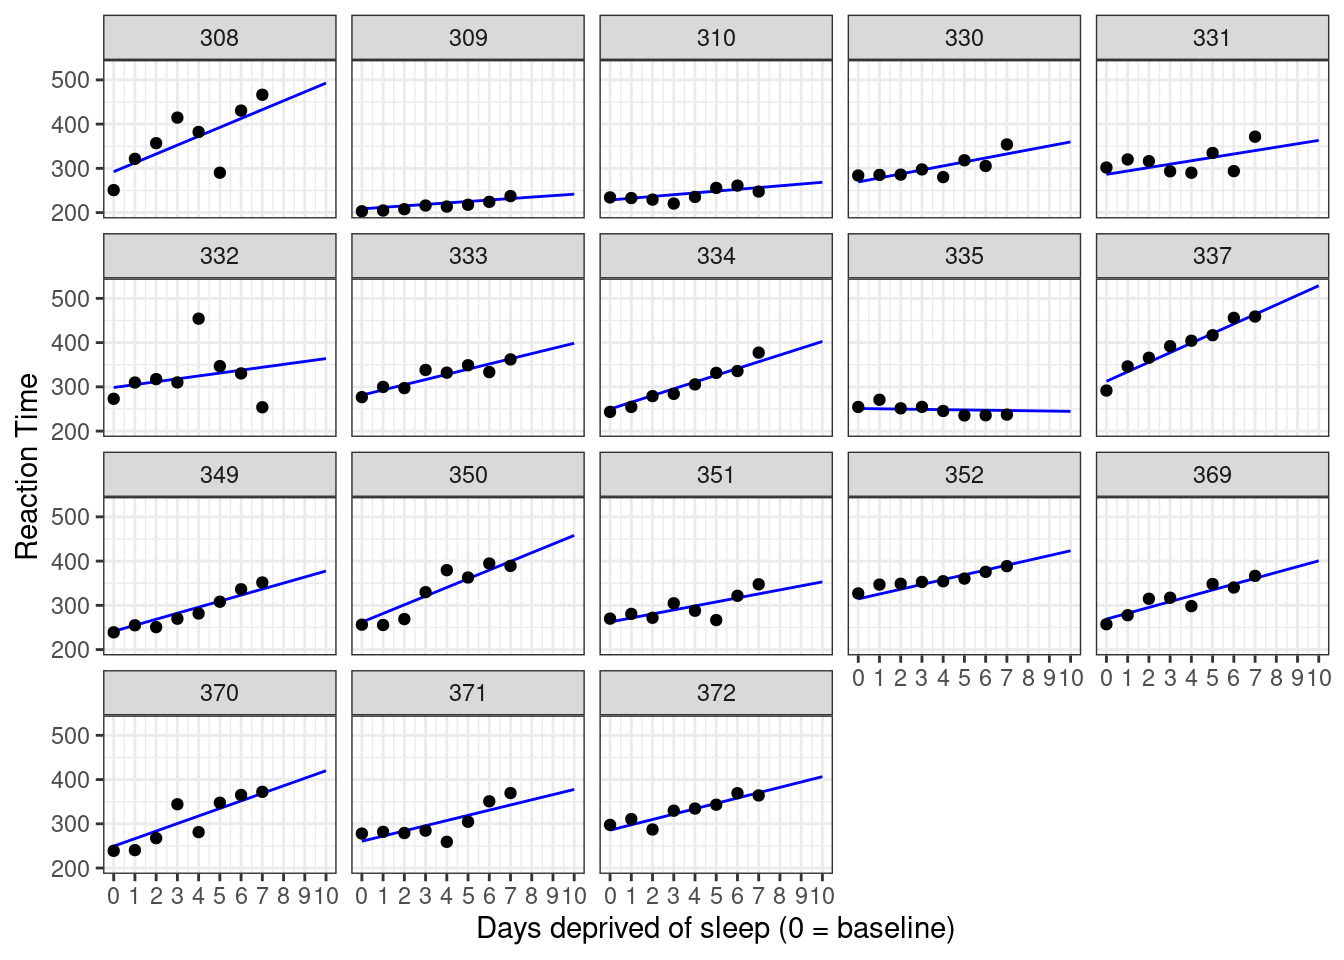
\includegraphics[width=1\linewidth]{05-linear-mixed-effects-intro_files/figure-latex/extrap-plot-1} 

}

\caption{Data against model with extrapolation.}\label{fig:extrap-plot}
\end{figure}

\hypertarget{multi-level-app}{%
\section{Multi-level app}\label{multi-level-app}}

\href{https://shiny.psy.gla.ac.uk/Dale/multilevel}{Try out the multi-level web app} to sharpen your understanding of the three different approaches to multi-level modeling.

\hypertarget{linear-mixed-effects-models-with-one-random-factor}{%
\chapter{Linear mixed-effects models with one random factor}\label{linear-mixed-effects-models-with-one-random-factor}}

\hypertarget{learning-objectives}{%
\section{Learning objectives}\label{learning-objectives}}

\begin{itemize}
\tightlist
\item
  understand how linear mixed-effects models can replace conventional analyses, and when they are appropriate
\item
  express various types of common designs in a regression framework
\item
  use model comparison (\texttt{anova()}) for testing effects
\item
  express various study designs using the R regression formula syntax
\end{itemize}

\hypertarget{when-and-why-would-you-want-to-replace-conventional-analyses-with-linear-mixed-effects-modeling}{%
\section{When, and why, would you want to replace conventional analyses with linear mixed-effects modeling?}\label{when-and-why-would-you-want-to-replace-conventional-analyses-with-linear-mixed-effects-modeling}}

We have repeatedly emphasized how many common techniques in psychology can be seen as special cases of the general linear model. This implies that it would be possible to replace these techniques with regression. In fact, you could analyze almost any conceivable dataset in psychology using one of the four functions below:

\begin{tabular}{l|l|l|l}
\hline
sampling design & type of data & function & description\\
\hline
single level & continuous, normally distributed & `base::lm()` & simple linear model\\
\hline
single level & count or categorical & `base::glm()` & generalized linear model\\
\hline
multilevel & continuous, normally distributed & `lme4::lmer()` & linear mixed-effects model\\
\hline
multilevel & count or categorical & `lme4::glmer()` & generalized linear mixed-effects model\\
\hline
\end{tabular}

To decide which function to use, you need to know the type of data you're working with (continuous and normally distributed, or not) and how the data have been sampled (single-level or multilevel). Arguments to these functions are highly similar across all four versions. We will learn about analyzing count and categorical data later in this course. For now, we will focus on continuous data, but many of the principles are identical.

Here is a comparison chart for single-level data (data where you don't have repeated-measures):

\begin{tabular}{l|l|l}
\hline
test & conventional approach & regression approach\\
\hline
one-sample t-test & `t.test(y, mu = c)` & `lm(y \textasciitilde{} 1, offset = c)`\\
\hline
independent samples t-test & `t.test(x, y)` & `lm(y \textasciitilde{} x)`\\
\hline
one factor ANOVA & `aov(y \textasciitilde{} x)` & `lm(y \textasciitilde{} x)`\\
\hline
factorial ANOVA & `aov(y \textasciitilde{} a * b)` & `lm(y \textasciitilde{} a * b)`\\
\hline
\end{tabular}

All of above designs are \emph{between-subjects} designs without repeated measures. (Note that in the factorial case, we would probably replace \texttt{a} and \texttt{b} with our own deviation-coded numerical predictors, for reasons already discussed in \href{interactions.html}{the chapter on interactions}).

Where mixed-effects models come into play is with multilevel data. Data is usually multilevel for one of the three reasons below (multiple reasons could simultaneously apply):

\begin{enumerate}
\def\labelenumi{\arabic{enumi}.}
\tightlist
\item
  you have a within-subject factor, and/or
\item
  you have \textbf{pseudoreplications}, and/or
\item
  you have multiple stimulus items (which we will discuss in the \href{linear-mixed-effects-models-with-crossed-random-factors.html}{next chapter}).
\end{enumerate}

(At this point, it would be a good idea to refresh your memory on the meaning of between- versus within- subject factors). In the \texttt{sleepstudy} data, you had the within-subject factor of \texttt{Day} (which is more a numeric variable, actually, than a factor; but it has multiple values varying within each participant).

\textbf{Pseudoreplications} occur when you take multiple measurements within the same condition. For instance, imagine a study where you randomly assign participants to consume one of two beverages---alcohol or water---before administering a simple response time task where they press a button as fast as possible when a light flashes. You would probably take more than one measurement of response time for each participant; let's assume that you measured it over 100 trials. You'd have one between-subject factor (beverage) and 100 observations per subject, for say, 20 subjects in each group. One common mistake novices make when analyzing such data is to try to run a t-test. \textbf{You can't directly use the conventional a t-test when you have pseudoreplications (or multiple stimuli).} You must first calculate means for each subject, and then run your analysis \textbf{on the means, not on the raw data.} There are versions of ANOVA that can deal with pseudoreplications, but you are probably better off using a linear-mixed effects model, which can better handle the complex dependency structure.

Here is a comparison chart for multi-level data:

\begin{tabular}{l|l|l}
\hline
test & conventional approach & regression approach\\
\hline
one-sample t-test with pseudoreplications & calculate means and use `t.test(x\_mean)` & <code>lmer(y \textasciitilde{} (1 | subject), offset = c)</code>\\
\hline
paired samples t-test, no pseudoreplications & `t.test(x, y, paired = TRUE)` & <code>lmer(y \textasciitilde{} x + (1 | subject))</code>\\
\hline
paired samples t-test with pseudoreplications & calculate means and use `t.test(x\_mean, y\_mean)` & <code>lmer(y \textasciitilde{} x + (1 + x | subject))</code>\\
\hline
repeated-measures ANOVA no pseudoreplications & `aov(y \textasciitilde{} x + Error(subject))` & <code>lmer(y \textasciitilde{} x + (1 | subject))</code>\\
\hline
repeated-measures ANOVA with pseudoreplications & `aov(y \textasciitilde{} x + Error(subject/x))` & <code>lmer(y \textasciitilde{} x + (1 + x | subject))</code>\\
\hline
factorial ANOVA, a \& b within, no pseudoreplications & `aov(y \textasciitilde{} a * b + Error(subject))` & <code>lmer(y \textasciitilde{} a * b + (1 | subject))</code>\\
\hline
factorial ANOVA with pseudoreplications & `aov(y \textasciitilde{} a * b + Error(subject/(a * b))` & <code>lmer(y \textasciitilde{} a * b + (1 + a * b | subject)</code>\\
\hline
\end{tabular}

One of the main selling points of the general linear models / regression framework over t-test and ANOVA is its flexibility. We saw this in the last chapter with the \texttt{sleepstudy} data, which could only be properly handled within a linear mixed-effects modelling framework. Despite the many advantages of regression, if you are in a situation where you have balanced data and can reasonably apply t-test or ANOVA without violating any of the assumptions behind the test, it makes sense to do so; these approaches have a long history in psychology and are more widely understood.

\hypertarget{example-independent-samples-t-test-on-multi-level-data}{%
\section{\texorpdfstring{Example: Independent-samples \(t\)-test on multi-level data}{Example: Independent-samples t-test on multi-level data}}\label{example-independent-samples-t-test-on-multi-level-data}}

Let's consider a situation where you are testing the effect of alcohol consumption on simple reaction time (e.g., press a button as fast as you can after a light appears). To keep it simple, let's assume that you have collected data from 14 participants randomly assigned to perform a set of 10 simple RT trials after one of two interventions: drinking a pint of alcohol (treatment condition) or a placebo drink (placebo condition). You have 7 participants in each of the two groups. Note that you would need more than this for a real study.

This \href{https://shiny.psy.gla.ac.uk/Dale/icc}{web app} presents simulated data from such a study. Subjects P01-P07 are from the placebo condition, while subjects T01-T07 are from the treatment condition. Please stop and have a look!

If we were going to run a t-test on these data, we would first need to calculate subject means, because otherwise the observations are not independent. You could do this as follows. (If you want to run the code below, you can download sample data from the web app above and save it as \texttt{independent\_samples.csv}).

\begin{Shaded}
\begin{Highlighting}[]
\KeywordTok{library}\NormalTok{(}\StringTok{"tidyverse"}\NormalTok{)}

\NormalTok{dat <-}\StringTok{ }\KeywordTok{read_csv}\NormalTok{(}\StringTok{"data/independent_samples.csv"}\NormalTok{, }\DataTypeTok{col_types =} \StringTok{"cci"}\NormalTok{)}

\NormalTok{subj_means <-}\StringTok{ }\NormalTok{dat }\OperatorTok
\StringTok{  }\KeywordTok{group_by}\NormalTok{(subject, cond) }\OperatorTok
\StringTok{  }\KeywordTok{summarise}\NormalTok{(}\DataTypeTok{mean_rt =} \KeywordTok{mean}\NormalTok{(RT)) }\OperatorTok
\StringTok{  }\KeywordTok{ungroup}\NormalTok{()}

\NormalTok{subj_means}
\end{Highlighting}
\end{Shaded}

\begin{verbatim}
## # A tibble: 14 x 3
##    subject cond  mean_rt
##    <chr>   <chr>   <dbl>
##  1 P01     P        354 
##  2 P02     P        384.
##  3 P03     P        391.
##  4 P04     P        404.
##  5 P05     P        421.
##  6 P06     P        392 
##  7 P07     P        400.
##  8 T08     T        430.
##  9 T09     T        432.
## 10 T10     T        410.
## 11 T11     T        455.
## 12 T12     T        450.
## 13 T13     T        418.
## 14 T14     T        489.
\end{verbatim}

Then, the \(t\)-test can be run using the ``formula'' version of \texttt{t.test()}.

\begin{Shaded}
\begin{Highlighting}[]
\KeywordTok{t.test}\NormalTok{(mean_rt }\OperatorTok{~}\StringTok{ }\NormalTok{cond, subj_means)}
\end{Highlighting}
\end{Shaded}

\begin{verbatim}
## 
## 	Welch Two Sample t-test
## 
## data:  mean_rt by cond
## t = -3.7985, df = 11.32, p-value = 0.002807
## alternative hypothesis: true difference in means is not equal to 0
## 95 percent confidence interval:
##  -76.32580 -20.44563
## sample estimates:
## mean in group P mean in group T 
##        392.3143        440.7000
\end{verbatim}

While there is nothing wrong with this analysis, aggregating the data throws away information. we can see in the above web app that there are actually two different sources of variability: trial-by-trial variability in simple RT (represented by \(\sigma\)) and variability across subjects in terms of their how slow or fast they are relative to the population mean (\(\gamma_{00}\)). The Data Generating Process for response time (\(Y_{st}\)) for subject \(s\) on trial \(t\) is shown below.

\emph{Level 1:}

\begin{equation}
Y_{st} = \beta_{0s} + \beta_{1} X_{s} + e_{st}
\end{equation}

\emph{Level 2:}

\begin{equation}
\beta_{0s} = \gamma_{00} + S_{0s}
\end{equation}

\begin{equation}
\beta_{1} = \gamma_{10}
\end{equation}

\emph{Variance Components:}

\begin{equation}
S_{0s} \sim N\left(0, {\tau_{00}}^2\right) 
\end{equation}

\begin{equation}
e_{st} \sim N\left(0, \sigma^2\right)
\end{equation}

In the above equation, \(X_s\) is a numerical predictor coding which condition the subject \(s\) is in; e.g., 0 for placebo, 1 for treatment.

The multi-level equations are somewhat cumbersome for such a simple model; we could just reduce levels 1 and 2 to

\begin{equation}
Y_{st} = \gamma_{00} + S_{0s} + \gamma_{10} X_s + e_{st},
\end{equation}

but it is worth becoming familiar with the multi-level format for when we encounter more complex designs.

Unlike the \texttt{sleepstudy} data seen in the last chapter, we only have one random effect for each subject, \(S_{0s}\). There is no random slope. Each subject appears in only one of the two treatment conditions, so it would not be possible to estimate how the effect of placebo versus alcohol varies over subjects. The mixed-effects model that we would fit to these data, with random intercepts but no random slopes, is known as a \textbf{random intercepts model}.

A random-intercepts model would adequately capture the two sources of variability mentioned above: the inter-subject variability in overall mean RT in the parameter \({\tau_{00}}^2\), and the trial-by-trial variability in the parameter \(\sigma^2\). We can calculate the proportion of the total variability attributable to individual differences among subjects using the formula below.

\[ICC = \frac{{\tau_{00}}^2}{{\tau_{00}}^2 + \sigma^2}\]

This quantity, known as the \textbf{intra-class correlation coefficient}, and tells you how much clustering there is in your data. It ranges from 0 to 1, with 0 indicating that all the variability is due to residual variance, and 1 indicating that all the variability is due to individual differences among subjects.

The lmer syntax for fitting a random intercepts model to the data is \texttt{lmer(RT\ \textasciitilde{}\ cond\ +\ (1\ \textbar{}\ subject),\ dat,\ REML=FALSE)}. Let's create our own numerical predictor first, to make it explicit that we are using dummy coding.

\begin{Shaded}
\begin{Highlighting}[]
\NormalTok{dat2 <-}\StringTok{ }\NormalTok{dat }\OperatorTok
\StringTok{  }\KeywordTok{mutate}\NormalTok{(}\DataTypeTok{cond_d =} \KeywordTok{if_else}\NormalTok{(cond }\OperatorTok{==}\StringTok{ "T"}\NormalTok{, 1L, 0L))}

\KeywordTok{distinct}\NormalTok{(dat2, cond, cond_d)  }\CommentTok{## double check}
\end{Highlighting}
\end{Shaded}

\begin{verbatim}
## # A tibble: 2 x 2
##   cond  cond_d
##   <chr>  <int>
## 1 P          0
## 2 T          1
\end{verbatim}

And now, estimate the model.

\begin{Shaded}
\begin{Highlighting}[]
\KeywordTok{library}\NormalTok{(}\StringTok{"lme4"}\NormalTok{)}

\NormalTok{mod <-}\StringTok{ }\KeywordTok{lmer}\NormalTok{(RT }\OperatorTok{~}\StringTok{ }\NormalTok{cond_d }\OperatorTok{+}\StringTok{ }\NormalTok{(}\DecValTok{1} \OperatorTok{|}\StringTok{ }\NormalTok{subject), dat2, }\DataTypeTok{REML =} \OtherTok{FALSE}\NormalTok{)}

\KeywordTok{summary}\NormalTok{(mod)}
\end{Highlighting}
\end{Shaded}

\begin{verbatim}
## Linear mixed model fit by maximum likelihood  ['lmerMod']
## Formula: RT ~ cond_d + (1 | subject)
##    Data: dat2
## 
##      AIC      BIC   logLik deviance df.resid 
##   1451.8   1463.5   -721.9   1443.8      136 
## 
## Scaled residuals: 
##      Min       1Q   Median       3Q      Max 
## -2.67117 -0.66677  0.01656  0.75361  2.58447 
## 
## Random effects:
##  Groups   Name        Variance Std.Dev.
##  subject  (Intercept)  329.3   18.15   
##  Residual             1574.7   39.68   
## Number of obs: 140, groups:  subject, 14
## 
## Fixed effects:
##             Estimate Std. Error t value
## (Intercept)  392.314      8.339  47.045
## cond_d        48.386     11.793   4.103
## 
## Correlation of Fixed Effects:
##        (Intr)
## cond_d -0.707
\end{verbatim}

Play around with the sliders in the app above and check the lmer output panel until you understand how the output maps onto the model parameters.

\hypertarget{when-is-a-random-intercepts-model-appropriate}{%
\subsection{When is a random-intercepts model appropriate?}\label{when-is-a-random-intercepts-model-appropriate}}

Of course, a mixed-effects model is only appropriate when you have multilevel data. The random-intercepts model is appropriate for any one-sample or between-subjects data with pseudoreplications (if you don't have pseudoreplications in this situation, you don't have multilevel data, and you can just use vanilla regression, e.g., \texttt{lm()}).

The ``random-intercepts-only'' model is also appropriate when you have within-subject factors in your design, but \textbf{only if you don't also have pseudoreplications}; that is, it is \textbf{only} appropriate when you have a single observation per subject per level of the within-subject factor. If you have more than one observation per subject per level/cell, you need to enrich your random effects structure with random slopes, as described in the next section. If the reason you have multiple observations per subject per level is because you have each subject reacting to the same set of stimuli, then you might want to consider a mixed-effects model with crossed random effects for subjects and stimuli, as described in the \href{linear-mixed-effects-models-with-crossed-random-factors.html}{next chapter}.

The same logic goes for factorial designs in which there is more than one within-subjects factor. In factorial designs, the random-intercepts model is appropriate if you have one observation per subject per \textbf{cell} formed by each combination of the within-subjects factors. For instance, if \(A\) and \(B\) are two two-level within-subject factors, you need to check that you have only one observation for each subject in \(A_1B_1\), \(A_1B_2\), \(A_2B_1\), and \(A_2B_2\). If you have more than one observation, you will need to consider including a random slope in your model.

\hypertarget{expressing-the-study-design-and-performing-tests-in-regression}{%
\section{Expressing the study design and performing tests in regression}\label{expressing-the-study-design-and-performing-tests-in-regression}}

In order to reproduce all of the t-test/ANOVA-style analyses in linear mixed-effects models, you'll need to better understand two things: (1) how to express your study design in a regression formula, and (2) how to get p-values for any tests you perform. The latter part is not obvious within the linear mixed-effects approach, since in many circumstances, the output of \texttt{lme4::lmer()} does not give you p-values by default, reflecting the fact that there are multiple options for deriving them \citep{Luke_2017}. Or, you might get p-values for individual regression coefficients, but the test you want to perform is a composite one where you need to test multiple parameters simultaneously.

First, let's take a closer look at the regression formula syntax in R and \textbf{\texttt{lme4}}. For the regression model \(y = \beta_0 + \beta_1 x_1 + \beta_2 x_2 + \ldots + \beta_m x_m + e\) with by-subject random effects you'd have:

\texttt{y\ \textasciitilde{}\ 1\ +\ x1\ +\ x2\ +\ ...\ +\ xm\ +\ (1\ +\ x1\ +\ ...\ \textbar{}\ subject)}

The residual term is implied and so not mentioned; only the predictors. The left side (before the tilde \texttt{\textasciitilde{}}) specifies the response variable, the right side has the predictor variables. The term in brackets, \texttt{(...\ \textbar{}\ ...)}, is specific to \textbf{\texttt{lme4}}. The right side of the vertical bar \texttt{\textbar{}} specifies the name of a variable (in this case, \texttt{subject}) that codes the levels of the random factor. The left side specifies what regression coefficients you want to allow to vary over those levels. The \texttt{1} at the start of the formula specifies that you want an intercept, which is included by default anyway, and so can be omitted. The \texttt{1} within the bracket specifies a \textbf{random intercept}, which is also included by default; the predictor variables mentioned inside the brackets specify \textbf{random slopes}. So you could write the above formula equivalently as:

\texttt{y\ \textasciitilde{}\ x1\ +\ x2\ +\ ...\ +\ xm\ +\ (x1\ +\ ...\ \textbar{}\ subject)}.

There is another important type of shortcut in R formulas, which we already saw in the \href{interactions.html}{chapter on interactions}; namely the ``star syntax'' \texttt{a\ *\ b} for specifying interactions. If you have two factors, \texttt{a} and \texttt{b} in your design, and you want all main effects and interactions in the model, you can use:

\texttt{y\ \textasciitilde{}\ a\ *\ b}

which is equivalent to \texttt{y\ \textasciitilde{}\ a\ +\ b\ +\ a:b} where \texttt{a} and \texttt{b} are the predictors coding main effects of A and B respectively, and \texttt{a:b} codes the AB interaction. It saves a lot of typing (and mistakes) to use the star syntax for interactions rather than spelling them out. This can be seen more easily in the example below, which codes a 2x2x2 factorial design including factors A, B, and C:

\texttt{y\ \textasciitilde{}\ a\ *\ b\ *\ c}

which is equivalent to

\texttt{y\ \textasciitilde{}\ a\ +\ b\ +\ c\ +\ a:b\ +\ a:c\ +\ b:c\ +\ a:b:c}

where \texttt{a:b}, \texttt{a:c}, and \texttt{b:c} are two-way interactions and \texttt{a:b:c} is the three-way interaction. You can use the star syntax inside the brackets for the random effects term as well, e.g.,

\texttt{y\ \textasciitilde{}\ a\ *\ b\ *\ c\ +\ (a\ *\ b\ *\ c\ \textbar{}\ subject)}

is equivalent to

\texttt{y\ \textasciitilde{}\ a\ +\ b\ +\ c\ +\ a:b\ +\ a:c\ +\ b:c\ +\ a:b:c\ +\ (a\ +\ b\ +\ c\ +\ a:b\ +\ a:c\ +\ b:c\ +\ a:b:c\ \textbar{}\ subject)}

which, despite its complexity, is a design that is not that uncommon in psychology (e.g., if you have all factors within and multiple stimuli per condition)!

\hypertarget{factors-with-more-than-two-levels}{%
\subsection{Factors with more than two levels}\label{factors-with-more-than-two-levels}}

As noted above, you could conduct a one-factor ANOVA in regression using the formula \texttt{lm(y\ \textasciitilde{}\ x)} for single-level or \texttt{lmer(y\ \textasciitilde{}\ x\ +\ (1\ \textbar{}\ subject))} for the multilevel version without pseudoreplications. In the formula, the \texttt{x} predictor would be of type \texttt{factor()}, which R would (by default) convert to \(k-1\) dummy-coded numerical predictors (one for each level; see the \href{interactions.html}{interaction chapter} for information).

It is often sensible to code your own numerical predictors, particularly if your goal is to do ANOVA-style tests of main effects and interactions, which can be difficult if any of your variables are of type \texttt{factor}. So for a design with one three-level factor called \texttt{meal} (\texttt{breakfast}, \texttt{lunch}, \texttt{dinner}) you could create two variables, \texttt{lunch\_v\_breakfast} and \texttt{dinner\_v\_breakfast} following the scheme below.

\begin{tabular}{l|r|r}
\hline
factor level & lunch\_v\_breakfast & dinner\_v\_breakfast\\
\hline
breakfast & -1/3 & -1/3\\
\hline
lunch & +2/3 & -1/3\\
\hline
dinner & -1/3 & +2/3\\
\hline
\end{tabular}

If your dependent variable is \texttt{calories}, your model would be:

\texttt{calories\ \textasciitilde{}\ lunch\_v\_breakfast\ +\ dinner\_v\_breakfast}.

But what if you wanted to interact \texttt{meal} with another two-level factor---say, \texttt{time\_of\_week} (\texttt{weekday} versus \texttt{weekend}, coded as -.5 and +.5 respectively), because you think the calories consumed per meal would differ across the levels of this variable? Then your model would be:

\texttt{calories\ \textasciitilde{}\ (lunch\_v\_breakfast\ +\ dinner\_v\_breakfast)\ *\ time\_of\_week}.

\href{interactions.html\#coding-schemes-for-categorical-variables}{(The inclusion of an interaction is the reason we chose the ``deviation'' coding scheme.)}. We put brackets around the predictors associated with the two-level variable so that each one interacts with \texttt{time\_of\_week}. The above star syntax is shorthand for:

\texttt{calories\ \textasciitilde{}\ lunch\_v\_breakfast\ +\ dinner\_v\_breakfast\ +\ time\_of\_week\ +\ lunch\_v\_breakfast:time\_of\_week\ +\ dinner\_v\_breakfast:time\_of\_week}.

This is the ``regression way'' of estimating parameters for a 3x2 factorial design.

\hypertarget{multiparameter-tests}{%
\subsection{Multiparameter tests}\label{multiparameter-tests}}

Whenever you are dealing with designs where all categorical factors have no more than two levels, the test of the regression coefficient associated with a given factor will be equivalent to the test for the effect in the ANOVA framework, provided you use \href{multiple-regression.html\#dealing-with-categorical-predictors}{sum or deviation coding}. But in the above example, we have a 3x2 design, with two predictor variables coding the main effect of \texttt{meal} (\texttt{lunch\_v\_breakfast} and \texttt{dinner\_v\_breakfast}). Let's simulate some data and run a one-factor ANOVA with \texttt{aov()}, and then we'll replicate the analysis using the regression function \texttt{lm()} (note that the same procedure works for mixed-effects models on multilevel data, just using \texttt{lme4::lmer()} instead of \texttt{base::lm()}).

\begin{Shaded}
\begin{Highlighting}[]
\CommentTok{## make up some data}
\KeywordTok{set.seed}\NormalTok{(}\DecValTok{62}\NormalTok{)}
\NormalTok{meals <-}\StringTok{ }\KeywordTok{tibble}\NormalTok{(}\DataTypeTok{meal =} \KeywordTok{factor}\NormalTok{(}\KeywordTok{rep}\NormalTok{(}\KeywordTok{c}\NormalTok{(}\StringTok{"breakfast"}\NormalTok{, }\StringTok{"lunch"}\NormalTok{, }\StringTok{"dinner"}\NormalTok{),}
                                  \DataTypeTok{each =} \DecValTok{6}\NormalTok{)),}
                \DataTypeTok{time_of_week =} \KeywordTok{factor}\NormalTok{(}\KeywordTok{rep}\NormalTok{(}\KeywordTok{rep}\NormalTok{(}\KeywordTok{c}\NormalTok{(}\StringTok{"weekday"}\NormalTok{, }\StringTok{"weekend"}\NormalTok{),}
                                              \DataTypeTok{each =} \DecValTok{3}\NormalTok{), }\DecValTok{3}\NormalTok{)),}
                \DataTypeTok{calories =} \KeywordTok{rnorm}\NormalTok{(}\DecValTok{18}\NormalTok{, }\DecValTok{450}\NormalTok{, }\DecValTok{50}\NormalTok{))}

\CommentTok{## use sum coding instead of default 'dummy' (treatment) coding}
\KeywordTok{options}\NormalTok{(}\DataTypeTok{contrasts =} \KeywordTok{c}\NormalTok{(}\DataTypeTok{unordered =} \StringTok{"contr.sum"}\NormalTok{, }\DataTypeTok{ordered =} \StringTok{"contr.poly"}\NormalTok{))}

\KeywordTok{aov}\NormalTok{(calories }\OperatorTok{~}\StringTok{ }\NormalTok{meal }\OperatorTok{*}\StringTok{ }\NormalTok{time_of_week, }\DataTypeTok{data =}\NormalTok{ meals) }\OperatorTok
\StringTok{  }\KeywordTok{summary}\NormalTok{()}
\end{Highlighting}
\end{Shaded}

\begin{verbatim}
##                   Df Sum Sq Mean Sq F value Pr(>F)
## meal               2   2164    1082   0.380  0.692
## time_of_week       1   5084    5084   1.783  0.207
## meal:time_of_week  2   4767    2384   0.836  0.457
## Residuals         12  34209    2851
\end{verbatim}

We get three \(F\)-tests, one for each main effect (\texttt{meal} and \texttt{time\_of\_week}) one for the interaction. What happens if we fit a model using \texttt{lm()}?

\begin{Shaded}
\begin{Highlighting}[]
\CommentTok{## add our own numeric predictors}
\NormalTok{meals2 <-}\StringTok{ }\NormalTok{meals }\OperatorTok
\StringTok{  }\KeywordTok{mutate}\NormalTok{(}\DataTypeTok{lunch_v_breakfast =} \KeywordTok{if_else}\NormalTok{(meal }\OperatorTok{==}\StringTok{ "lunch"}\NormalTok{, }\DecValTok{2}\OperatorTok{/}\DecValTok{3}\NormalTok{, }\DecValTok{-1}\OperatorTok{/}\DecValTok{3}\NormalTok{),}
         \DataTypeTok{dinner_v_breakfast =} \KeywordTok{if_else}\NormalTok{(meal }\OperatorTok{==}\StringTok{ "dinner"}\NormalTok{, }\DecValTok{2}\OperatorTok{/}\DecValTok{3}\NormalTok{, }\DecValTok{-1}\OperatorTok{/}\DecValTok{3}\NormalTok{),}
         \DataTypeTok{time_week =} \KeywordTok{if_else}\NormalTok{(time_of_week }\OperatorTok{==}\StringTok{ "weekend"}\NormalTok{, }\DecValTok{1}\OperatorTok{/}\DecValTok{2}\NormalTok{, }\DecValTok{-1}\OperatorTok{/}\DecValTok{2}\NormalTok{))}

\CommentTok{## double check our coding}
\KeywordTok{distinct}\NormalTok{(meals2, meal, time_of_week,}
\NormalTok{         lunch_v_breakfast, dinner_v_breakfast, time_week)}

\CommentTok{## fit regression model}
\NormalTok{mod <-}\StringTok{ }\KeywordTok{lm}\NormalTok{(calories }\OperatorTok{~}\StringTok{ }\NormalTok{(lunch_v_breakfast }\OperatorTok{+}\StringTok{ }\NormalTok{dinner_v_breakfast) }\OperatorTok{*}
\StringTok{            }\NormalTok{time_week, }\DataTypeTok{data =}\NormalTok{ meals2)}

\KeywordTok{summary}\NormalTok{(mod)}
\end{Highlighting}
\end{Shaded}

\begin{verbatim}
## # A tibble: 6 x 5
##   meal      time_of_week lunch_v_breakfast dinner_v_breakfast time_week
##   <fct>     <fct>                    <dbl>              <dbl>     <dbl>
## 1 breakfast weekday                 -0.333             -0.333      -0.5
## 2 breakfast weekend                 -0.333             -0.333       0.5
## 3 lunch     weekday                  0.667             -0.333      -0.5
## 4 lunch     weekend                  0.667             -0.333       0.5
## 5 dinner    weekday                 -0.333              0.667      -0.5
## 6 dinner    weekend                 -0.333              0.667       0.5
## 
## Call:
## lm(formula = calories ~ (lunch_v_breakfast + dinner_v_breakfast) * 
##     time_week, data = meals2)
## 
## Residuals:
##     Min      1Q  Median      3Q     Max 
## -68.522 -35.895  -4.063  42.061  73.081 
## 
## Coefficients:
##                              Estimate Std. Error t value Pr(>|t|)    
## (Intercept)                    451.15      12.58  35.848 1.42e-13 ***
## lunch_v_breakfast              -25.23      30.83  -0.818    0.429    
## dinner_v_breakfast             -20.59      30.83  -0.668    0.517    
## time_week                       33.61      25.17   1.335    0.207    
## lunch_v_breakfast:time_week    -58.31      61.65  -0.946    0.363    
## dinner_v_breakfast:time_week    17.93      61.65   0.291    0.776    
## ---
## Signif. codes:  0 '***' 0.001 '**' 0.01 '*' 0.05 '.' 0.1 ' ' 1
## 
## Residual standard error: 53.39 on 12 degrees of freedom
## Multiple R-squared:  0.2599,	Adjusted R-squared:  -0.04843 
## F-statistic: 0.843 on 5 and 12 DF,  p-value: 0.5447
\end{verbatim}

OK, this output looks very different! How do you perform ANOVA-like tests in those situations? You have estimates for \texttt{lunch\_v\_breakfast} and \texttt{dinner\_v\_breakfast} but how would you convert this into a single test for the main effect of \texttt{meal}? Likewise, you have two interaction terms, \texttt{lunch\_v\_breakfast:tow} and \texttt{dinner\_v\_breakfast:tow}; how do you convert this into a single test for the interaction?

The solution is to perform \textbf{multiparameter tests} using model comparison, implemented by the \texttt{anova()} function in R. To test for the main effect of \texttt{meal}, you'd compare a model containing the two predictor variables coding that factor (\texttt{lunch\_v\_breakfast} and \texttt{dinner\_v\_breakfast}) to a model excluding these two predictors but that is otherwise identical. You can either re-fit the model by writing it out and excluding the terms, or by using the \texttt{update()} function and removing the terms (which is a shortcut). Let's write it out first.

\begin{Shaded}
\begin{Highlighting}[]
\CommentTok{## fit the model}
\NormalTok{mod_main_eff <-}\StringTok{ }\KeywordTok{lm}\NormalTok{(calories }\OperatorTok{~}\StringTok{ }\NormalTok{time_week }\OperatorTok{+}
\StringTok{                     }\NormalTok{lunch_v_breakfast}\OperatorTok{:}\NormalTok{time_week }\OperatorTok{+}\StringTok{ }\NormalTok{dinner_v_breakfast}\OperatorTok{:}\NormalTok{time_week,}
\NormalTok{                   meals2)}

\CommentTok{## compare models}
\KeywordTok{anova}\NormalTok{(mod, mod_main_eff)}
\end{Highlighting}
\end{Shaded}

\begin{verbatim}
## Analysis of Variance Table
## 
## Model 1: calories ~ (lunch_v_breakfast + dinner_v_breakfast) * time_week
## Model 2: calories ~ time_week + lunch_v_breakfast:time_week + dinner_v_breakfast:time_week
##   Res.Df   RSS Df Sum of Sq      F Pr(>F)
## 1     12 34209                           
## 2     14 36373 -2   -2163.9 0.3795 0.6921
\end{verbatim}

OK, now here is an equivalent version using the shortcut \texttt{update()} function, which takes the model you want to update as the first argument and then a special syntax for the formula including your changes. For the formula, we use \texttt{.\ \textasciitilde{}\ .\ -lunch\_v\_breakfast\ -dinner\_v\_breakfast\textasciitilde{}} Although this formula seems weird, the dot \texttt{.} says ``keep everything on this side of the model formula (left of \texttt{\textasciitilde{}}) as it is in the original model.'' So the formula \texttt{.\ \textasciitilde{}\ .} would use the same formula as the original model; that is, \texttt{update(mod,\ .\ \textasciitilde{}\ .)} would fit the exact same model as above. In contrast, \texttt{.\ \textasciitilde{}\ .\ -x\ -y} means "everything the same on the left side (same DV), but remove variables \texttt{x} and \texttt{y} from the right side.

\begin{Shaded}
\begin{Highlighting}[]
\NormalTok{mod_main_eff2 <-}\StringTok{ }\KeywordTok{update}\NormalTok{(mod, . }\OperatorTok{~}\StringTok{ }\NormalTok{. }\OperatorTok{-}\NormalTok{lunch_v_breakfast }\OperatorTok{-}\NormalTok{dinner_v_breakfast)}

\KeywordTok{anova}\NormalTok{(mod, mod_main_eff2)}
\end{Highlighting}
\end{Shaded}

\begin{verbatim}
## Analysis of Variance Table
## 
## Model 1: calories ~ (lunch_v_breakfast + dinner_v_breakfast) * time_week
## Model 2: calories ~ time_week + lunch_v_breakfast:time_week + dinner_v_breakfast:time_week
##   Res.Df   RSS Df Sum of Sq      F Pr(>F)
## 1     12 34209                           
## 2     14 36373 -2   -2163.9 0.3795 0.6921
\end{verbatim}

As you can see, this gives us the same result as above.

If we want to test the main effect of \texttt{time\_of\_week}, we remove that predictor.

\begin{Shaded}
\begin{Highlighting}[]
\NormalTok{mod_tow <-}\StringTok{ }\KeywordTok{update}\NormalTok{(mod, . }\OperatorTok{~}\StringTok{ }\NormalTok{. }\OperatorTok{-}\NormalTok{time_week)}

\KeywordTok{anova}\NormalTok{(mod, mod_tow)}
\end{Highlighting}
\end{Shaded}

\begin{verbatim}
## Analysis of Variance Table
## 
## Model 1: calories ~ (lunch_v_breakfast + dinner_v_breakfast) * time_week
## Model 2: calories ~ lunch_v_breakfast + dinner_v_breakfast + lunch_v_breakfast:time_week + 
##     dinner_v_breakfast:time_week
##   Res.Df   RSS Df Sum of Sq      F Pr(>F)
## 1     12 34209                           
## 2     13 39294 -1   -5084.1 1.7834 0.2065
\end{verbatim}

Try to figure out how to test the interaction on your own.

Click to see solution

\begin{Shaded}
\begin{Highlighting}[]
\NormalTok{mod_interact <-}\StringTok{ }\KeywordTok{update}\NormalTok{(mod, . }\OperatorTok{~}\StringTok{ }\NormalTok{. }\OperatorTok{-}\NormalTok{lunch_v_breakfast}\OperatorTok{:}\NormalTok{time_week}
                       \OperatorTok{-}\NormalTok{dinner_v_breakfast}\OperatorTok{:}\NormalTok{time_week)}

\KeywordTok{anova}\NormalTok{(mod, mod_interact)}
\end{Highlighting}
\end{Shaded}

\begin{verbatim}
## Analysis of Variance Table
## 
## Model 1: calories ~ (lunch_v_breakfast + dinner_v_breakfast) * time_week
## Model 2: calories ~ lunch_v_breakfast + dinner_v_breakfast + time_week
##   Res.Df   RSS Df Sum of Sq      F Pr(>F)
## 1     12 34209                           
## 2     14 38977 -2   -4767.4 0.8362 0.4571
\end{verbatim}

We got the exact same results doing model comparison with \texttt{lm()} as we did using \texttt{aov()}. Although this involved more steps, it is worth learning this approach as it will ultimately give you much more flexibility.

\hypertarget{linear-mixed-effects-models-with-crossed-random-factors}{%
\chapter{Linear mixed-effects models with crossed random factors}\label{linear-mixed-effects-models-with-crossed-random-factors}}

\hypertarget{learning-objectives}{%
\section{Learning objectives}\label{learning-objectives}}

\begin{itemize}
\tightlist
\item
  analyze data from a design with crossed random factors of subjects and stimuli
\item
  appropriately specify random effects to enable proper generalization
\item
  simulate data for a design with crossed random factors
\end{itemize}

\hypertarget{web-app}{%
\section{Web app}\label{web-app}}

\begin{itemize}
\tightlist
\item
  \href{https://shiny.psy.gla.ac.uk/Dale/crossed}{Demo of crossed random effects}
\end{itemize}

\hypertarget{generalizing-over-encounters-between-subjects-and-stimuli}{%
\section{Generalizing over encounters between subjects and stimuli}\label{generalizing-over-encounters-between-subjects-and-stimuli}}

A common goal of experiments in psychology is to test claims about behavior that arises in response to certain types of stimuli (or sometimes, the neural underpinning of that behavior). The stimuli might be, for instance, words, images, sounds, videos, or stories. Some examples of claims you might want to test are:

\begin{itemize}
\tightlist
\item
  when listening to words in a second language, do bilinguals experience interference from words in their native language?
\item
  do people rate the attractiveness of faces differently when they are in a good mood than when they are in a bad mood?
\item
  does viewing soothing images help reduce stress relative to more neutral images?
\item
  when reading a scenario ambiguously describing a target individual, are people more likely to make assumptions about what social group the target belongs to after being subliminally primed?
\end{itemize}

One thing to note about all these claims is that the are of the type, ``what happens to our measurements when an individual of type X encounters a stimulus of type Y'', where X is drawn from a target population of subjects and Y is drawn from a target population of stimuli. In other words, we are attempt to make generalizable claims about a particular class of \textbf{events} involving \textbf{encounters} between sampling units of subjects and stimuli \citep{Barr_2017}. But just like we can't sample all possible subjects from the target population of subjects, we also cannot sample all possible stimuli from the target population of stimuli. Thus, when drawing inferences, we need to account for the uncertainty introduced in our estimates by \emph{both} sampling processes \citep{Coleman_1964, Clark_1973, Judd_Westfall_Kenny_2012, yarkoni_2019}. Linear mixed-effects models make it particularly easy to do this by allowing more than one random factor in our model formula \citep{Baayen_Davidson_Bates_2008}.

Here is a simple example of a study where you are interested in testing whether people rate pictures of cats, dogs, or sunsets as more soothing images to look at. You want to say something general about the category of cats, dogs, and sunsets and not something about the specific pictures that you happened to sample. Let's say you randomly select four images from each of the three categories from Google Images (you would absolutely need to have more to be able to say something generalizable, but we chose a small number to keep the example simple). So your table of stimuli might look like the following:

\begin{tabular}{r|l|l}
\hline
stimulus\_id & category & file\\
\hline
1 & cat & cat1.jpg\\
\hline
2 & cat & cat2.jpg\\
\hline
3 & cat & cat3.jpg\\
\hline
4 & cat & cat4.jpg\\
\hline
5 & dog & dog1.jpg\\
\hline
6 & dog & dog2.jpg\\
\hline
7 & dog & dog3.jpg\\
\hline
8 & dog & dog4.jpg\\
\hline
9 & sunset & sunset1.jpg\\
\hline
10 & sunset & sunset2.jpg\\
\hline
11 & sunset & sunset3.jpg\\
\hline
12 & sunset & sunset4.jpg\\
\hline
\end{tabular}

Then you sample a set of four participants to perform the soothing ratings. Again, four would be too few for a real study, but we're keeping it small just for expository purposes.

\begin{tabular}{r|r|l}
\hline
subject\_id & age & date\\
\hline
1 & 67 & 2020-05-01\\
\hline
2 & 68 & 2020-05-13\\
\hline
3 & 55 & 2020-05-17\\
\hline
4 & 24 & 2020-05-26\\
\hline
\end{tabular}

Now, because each subject has given a ``soothingness'' rating for each picture, you'd have a full dataset consisting of all of the levels of \texttt{subject\_id} crossed with all of the levels of \texttt{stimulus\_id}. This is what we mean when we talk about ``crossed random factors.'' You can create the table containing all these combinations with the \texttt{crossing()} function from \texttt{tidyr} (which is loaded when you load in \texttt{tidyverse}).

\begin{Shaded}
\begin{Highlighting}[]
\KeywordTok{crossing}\NormalTok{(subjects }\OperatorTok\StringTok{ }\KeywordTok{select}\NormalTok{(subject_id),}
\NormalTok{         stimuli }\OperatorTok\StringTok{ }\KeywordTok{select}\NormalTok{(}\OperatorTok{-}\NormalTok{category)) }
\end{Highlighting}
\end{Shaded}

\begin{tabular}{r|r|l}
\hline
subject\_id & stimulus\_id & file\\
\hline
1 & 1 & cat1.jpg\\
\hline
1 & 2 & cat2.jpg\\
\hline
1 & 3 & cat3.jpg\\
\hline
1 & 4 & cat4.jpg\\
\hline
1 & 5 & dog1.jpg\\
\hline
1 & 6 & dog2.jpg\\
\hline
1 & 7 & dog3.jpg\\
\hline
1 & 8 & dog4.jpg\\
\hline
1 & 9 & sunset1.jpg\\
\hline
1 & 10 & sunset2.jpg\\
\hline
1 & 11 & sunset3.jpg\\
\hline
1 & 12 & sunset4.jpg\\
\hline
2 & 1 & cat1.jpg\\
\hline
2 & 2 & cat2.jpg\\
\hline
2 & 3 & cat3.jpg\\
\hline
2 & 4 & cat4.jpg\\
\hline
2 & 5 & dog1.jpg\\
\hline
2 & 6 & dog2.jpg\\
\hline
2 & 7 & dog3.jpg\\
\hline
2 & 8 & dog4.jpg\\
\hline
2 & 9 & sunset1.jpg\\
\hline
2 & 10 & sunset2.jpg\\
\hline
2 & 11 & sunset3.jpg\\
\hline
2 & 12 & sunset4.jpg\\
\hline
3 & 1 & cat1.jpg\\
\hline
3 & 2 & cat2.jpg\\
\hline
3 & 3 & cat3.jpg\\
\hline
3 & 4 & cat4.jpg\\
\hline
3 & 5 & dog1.jpg\\
\hline
3 & 6 & dog2.jpg\\
\hline
3 & 7 & dog3.jpg\\
\hline
3 & 8 & dog4.jpg\\
\hline
3 & 9 & sunset1.jpg\\
\hline
3 & 10 & sunset2.jpg\\
\hline
3 & 11 & sunset3.jpg\\
\hline
3 & 12 & sunset4.jpg\\
\hline
4 & 1 & cat1.jpg\\
\hline
4 & 2 & cat2.jpg\\
\hline
4 & 3 & cat3.jpg\\
\hline
4 & 4 & cat4.jpg\\
\hline
4 & 5 & dog1.jpg\\
\hline
4 & 6 & dog2.jpg\\
\hline
4 & 7 & dog3.jpg\\
\hline
4 & 8 & dog4.jpg\\
\hline
4 & 9 & sunset1.jpg\\
\hline
4 & 10 & sunset2.jpg\\
\hline
4 & 11 & sunset3.jpg\\
\hline
4 & 12 & sunset4.jpg\\
\hline
\end{tabular}

Because you have 4 subjects responding to 12 stimuli, the resulting table will have 48 rows.

\hypertarget{lme4-syntax-for-crossed-random-factors}{%
\section{lme4 syntax for crossed random factors}\label{lme4-syntax-for-crossed-random-factors}}

How should we analyze such data? Recall from the last chapter that the lme4 formula syntax for a model with by-subject random intercepts and slopes for predictor \texttt{x} would be given by \texttt{y\ \textasciitilde{}\ x\ +\ (1\ +\ x\ \textbar{}\ subject\_id)} where the term in brackets with the vertical bar \texttt{\textbar{}} provides the random effects specification. The variable to the right of the bar, \texttt{subject\_id}, specifies the variable that identifies the levels of the random factor. The formula to the left of the bar within the brackets, \texttt{1\ +\ x}, specifies the random effects associated with this factor, which in this case is a random intercept and random slope for \texttt{x}. The best way to think about this bracketed part of the formula \texttt{(1\ +\ x\ \textbar{}\ subject\_id)} is \textbf{as an instruction to \texttt{lme4::lmer()} about how to build a covariance matrix capturing the variance introduced by the random factor of subjects.} By now you should realize that this instruction would result in the estimation of a two-dimensional covariance matrix, with one dimension for intercept variance and one for slope variance.

But we are not limited to the estimation of random effects for subjects; we can also specify the estimation of random effects for stimuli by simply adding another term to the formula. For example,

\texttt{y\ \textasciitilde{}\ x\ +\ (1\ +\ x\ \textbar{}\ subject\_id)\ +\ (1\ +\ x\ \textbar{}\ stimulus\_id)}

regresses \texttt{y} on \texttt{x} with by-subject random intercepts and slopes and by-stimulus random intercepts. In this way, the fitted model will capture two sources of uncertainty about our estimates---the uncertainty introduced by sampling subjects as well as the uncertainty introduced by sampling items. Now we are estimating \textbf{two independent covariance matrices}, one for subjects and one for items. In the above example, both of these matrices will have the same 2x2 structure, but this need not be the case. We can flexibly change the random effects structure by changing the formula specification on the left side of each bar \texttt{\textbar{}} symbol. For instance, if we have another predictor \texttt{w}, we might have:

\texttt{y\ \textasciitilde{}\ x\ +\ (x\ \textbar{}\ subject\_id)\ +\ (x\ +\ w\ \textbar{}\ stimulus\_id)}

which would estimate the same 2x2 matrix for subjects, but the covariance matrix for stimuli would now be a 3x3 matrix (intercepts, slope of x, and slope of w). Although this enables great flexibility, as the random effects structure becomes more complex, the estimation process becomes more difficult and less likely to converge upon a result.

\hypertarget{specifying-random-effects}{%
\section{Specifying random effects}\label{specifying-random-effects}}

The choice of random effects structure is not a new problem that appeared with linear mixed-effects models. In traditional approaches using t-test and ANOVA, you choose the random effects structure implicitly when you choose what procedure to use. As discussed in the last chapter, if you choose a paired samples t-test over an independent samples t-test, that is analogous to choosing to fit \texttt{lme4::lmer(y\ \textasciitilde{}\ x\ +\ (1\ \textbar{}\ subject))} over \texttt{lm(y\ \textasciitilde{}\ x)}. Likewise, you can run a mixed model ANOVA as either \texttt{aov(y\ \textasciitilde{}\ x\ +\ Error(subject\_id))}, which is equivalent to a random intercepts model, or \texttt{aov(y\ \textasciitilde{}\ x\ +\ Error(x\ /\ subject\_id))}, which is equivalent to a random slopes model. The tradition in psychology when performing confirmatory analyses is to use the \emph{maximal random effects structure justified by the design of your study}. So, if you have one-factor data with pseudoreplications, you would use \texttt{aov(y\ \textasciitilde{}\ x\ +\ Error(x\ /\ subject\_id))} rather than \texttt{aov(y\ \textasciitilde{}\ x\ +\ Error(subject\_id))}. Analogously, if you were to analyze the same data with pseudoreplications using a linear mixed effects model, you should use \texttt{lme4::lmer(y\ \textasciitilde{}\ x\ +\ (1\ +\ x\ \textbar{}\ subject\_id))} rather than \texttt{lme4::lmer(y\ \textasciitilde{}\ x\ +\ (1\ \textbar{}\ subject\_id))}. In other words, you should account for all sources of non-independence introduced by repeated sampling from the same subjects or stimuli. This approach is known as the \textbf{maximal random effects} approach or the \textbf{design-driven approach} to specifying random effects structure \citep{Barr_et_al_2013}. Failing to account for dependencies introduced by the design is likely to lead to standard errors that are too small, which in turn, lead to p-values that are smaller than they should be, and thus, higher false positive (Type I error) rates. In some cases, it can lead to lower power, and thus a higher false negative (Type II error) rate. It is thus of critical importance to pay close attention to the random effects structure when performing analyses.

Linear mixed-effects models almost inevitably include random intercepts for any random factor included in the design. So if your random factors are subjects and stimuli identified by \texttt{subject\_id} and \texttt{stimulus\_id} respectively, then at the very least, your model syntax will include \texttt{(1\ \textbar{}\ subject\_id)\ +\ (1\ \textbar{}\ stimulus\_id)}. But you will have various predictors in the model, so key question becomes: what predictors should I allow to vary over what sampling units? For instance, if the fixed-effects part of your model is a 2x2 factorial design with factors A and B, \texttt{y\ \textasciitilde{}\ a\ *\ b\ +\ ...}, you could have a large variety of random effects structures, including (but not limited to):

\begin{enumerate}
\def\labelenumi{\arabic{enumi}.}
\tightlist
\item
  random intercepts only: \texttt{y\ \textasciitilde{}\ a\ *\ b\ +\ (1\ \textbar{}\ subject\_id)\ +\ (1\ \textbar{}\ stimulus\_id)}
\item
  by-subjects random intercepts for a and by-stimulus random intercepts: \texttt{y\ \textasciitilde{}\ a\ *\ b\ +\ (a\ \textbar{}\ subject\_id)\ +\ (1\ \textbar{}\ stimulus\_id)}
\item
  by-subjects random intercepts and slopes for a and b and the ab interaction, with by-stimulus random intercepts: \texttt{y\ \textasciitilde{}\ a\ *\ b\ +\ (a\ *\ b\ \textbar{}\ subject\_id)\ +\ (1\ \textbar{}\ stimulus\_id)}
\item
  by-subjects random intercepts and slopes for a and b and the ab interaction, by-stimulus random intercepts and slopes for a and b and the ab interaction, \texttt{y\ \textasciitilde{}\ a\ *\ b\ +\ (a\ *\ b\ \textbar{}\ subject\_id)\ +\ (a\ *\ b\ \textbar{}\ stimulus\_id)}.
\end{enumerate}

It is important to be clear about one thing.

The ``maximal random effects structure justified by the design'' is not the same as the ``maximum possible random effects structure''; that is, it does not entail automatically putting in all random slopes for all random factors for all predictors in your model. You have to follow the guidelines for random effects in the next section to decide whether inclusion of a particular random slope is, in fact, ``justified by the design.''

Some authors suggest a ``data-driven'' alternative to design-driven random effects, suggesting that researchers should only include random slopes justified by the design if they are further justified by the data \citep{Matuschek_et_al_2017}. For example, you might use a null-hypothesis test to determine whether including a by-subject random slope for \texttt{x} significantly improves the model fit, and only include that effect if it does. Although this could potentially improve power for the test of theoretical interest when random slopes are very small, it also exposes you to additional unknown risk of false positives, so it is questionable whether this the right approach in a confirmatory context. Thus, we do not recommend a data-driven approach.

\hypertarget{rules-for-choosing-random-effects-for-categorical-factors}{%
\subsection{Rules for choosing random effects for categorical factors}\label{rules-for-choosing-random-effects-for-categorical-factors}}

The random effects structure for a linear mixed-effects model---in other words, your assumptions about what effects vary over what sampling units---is absolutely critical for ensuring that your parameters reflect the uncertainty introduced by sampling \citep{Barr_et_al_2013}. First off, note that we are focused on predictors representing \textbf{design variables} that are of theoretical interest and on which you will perform inferential tests. If you have predictors that represent \textbf{control variables}, over which you do not intend to perform statistical tests, it is unlikely that random slopes are needed.

The following rules are derived from \citet{Barr_et_al_2013} and \citet{Barr_2013}. Consult these papers if you wish to find out more about these guidelines. Keep in mind that you can only use a mixed effects model if you have repeated measures data, either because of pseudoreplications and/or the presence of within-subject (or within-stimulus) factors. With crossed random factors, you inevitably have pseudoreplications---multiple observations per subject due to multiple stimuli, multiple observations per stimulus due to multiple subjects. The key to determining random effects structure is figuring out which factors are within-subjects or within-stimuli, and where any pseudoreplications are located in the design. You apply the rules once for subjects to determine the form of the \texttt{(1\ +\ ...\ \textbar{}\ subject\_id)} part of the formula, and once for stimuli to determine the form of the \texttt{(1\ +\ ...\ \textbar{}\ stimulus\_id)} part of the formula. Where you see the word ``unit'' or ``sampling unit'' below, substitute ``subject'' or ``stimuli'' as needed.

Here are the rules:

\begin{enumerate}
\def\labelenumi{\arabic{enumi}.}
\tightlist
\item
  If there are repeated measures on sampling units, you need a random intercept for that random factor: \texttt{(1\ \textbar{}\ unit\_id)};
\item
  If a factor \texttt{x} is between-unit, you do not need a random slope for that factor;
\item
  Determine the highest order interaction of within-subject factors for the unit under consideration. If you have pseudoreplications within each cell defined by those combinations (i.e., multiple observations per cell), then for that unit you will need a slope for that interaction as well as for all lower order effects. If there are no pseudoreplications, then you do not need any random slopes.
\end{enumerate}

The first two rules are straightforward, but the third requires some explanation. Let's first ask: how do we know whether some factor is between or within unit?

A simple way to determine whether a factor is between or within is to use the \texttt{dplyr::count()} function, which gives frequency counts, and which is loaded when you load tidyverse. Let's say you are interested in whether factor \(A\) is within or between subjects, for the imaginary 2x2x2 factorial data \texttt{abc\_data} below where \(A\), \(B\), and \(C\) name the factors of your design.

\begin{Shaded}
\begin{Highlighting}[]
\KeywordTok{library}\NormalTok{(}\StringTok{"tidyverse"}\NormalTok{)}

\CommentTok{## run this code to create the table "abc_data"}
\NormalTok{abc_subj <-}\StringTok{ }\KeywordTok{tibble}\NormalTok{(}\DataTypeTok{subject_id =} \DecValTok{1}\OperatorTok{:}\DecValTok{4}\NormalTok{,}
                   \DataTypeTok{B =} \KeywordTok{rep}\NormalTok{(}\KeywordTok{c}\NormalTok{(}\StringTok{"B1"}\NormalTok{, }\StringTok{"B2"}\NormalTok{), }\DataTypeTok{times =} \DecValTok{2}\NormalTok{))}

\NormalTok{abc_item  <-}\StringTok{ }\KeywordTok{tibble}\NormalTok{(}\DataTypeTok{stimulus_id =} \DecValTok{1}\OperatorTok{:}\DecValTok{4}\NormalTok{,}
                    \DataTypeTok{A =} \KeywordTok{rep}\NormalTok{(}\KeywordTok{c}\NormalTok{(}\StringTok{"A1"}\NormalTok{, }\StringTok{"A2"}\NormalTok{), }\DataTypeTok{each =} \DecValTok{2}\NormalTok{),}
                    \DataTypeTok{C =} \KeywordTok{rep}\NormalTok{(}\KeywordTok{c}\NormalTok{(}\StringTok{"C1"}\NormalTok{, }\StringTok{"C2"}\NormalTok{), }\DataTypeTok{times =} \DecValTok{2}\NormalTok{))}

\NormalTok{abc_data <-}\StringTok{ }\KeywordTok{crossing}\NormalTok{(abc_subj, abc_item) }\OperatorTok
\StringTok{  }\KeywordTok{select}\NormalTok{(subject_id, stimulus_id, }\KeywordTok{everything}\NormalTok{())}
\end{Highlighting}
\end{Shaded}

To see whether \(A\) is within or between subjects, use:

\begin{Shaded}
\begin{Highlighting}[]
\NormalTok{abc_data }\OperatorTok
\StringTok{  }\KeywordTok{count}\NormalTok{(subject_id, A)}
\end{Highlighting}
\end{Shaded}

\begin{verbatim}
## # A tibble: 8 x 3
##   subject_id A         n
##        <int> <chr> <int>
## 1          1 A1        2
## 2          1 A2        2
## 3          2 A1        2
## 4          2 A2        2
## 5          3 A1        2
## 6          3 A2        2
## 7          4 A1        2
## 8          4 A2        2
\end{verbatim}

In the resulting table, you can see that each subject gets both levels of \(A\), making it a within-subject factor. What about \(B\) and \(C\)?

\begin{Shaded}
\begin{Highlighting}[]
\NormalTok{abc_data }\OperatorTok
\StringTok{  }\KeywordTok{count}\NormalTok{(subject_id, B)}
\end{Highlighting}
\end{Shaded}

\begin{verbatim}
## # A tibble: 4 x 3
##   subject_id B         n
##        <int> <chr> <int>
## 1          1 B1        4
## 2          2 B2        4
## 3          3 B1        4
## 4          4 B2        4
\end{verbatim}

\begin{Shaded}
\begin{Highlighting}[]
\NormalTok{abc_data }\OperatorTok
\StringTok{  }\KeywordTok{count}\NormalTok{(subject_id, C)}
\end{Highlighting}
\end{Shaded}

\begin{verbatim}
## # A tibble: 8 x 3
##   subject_id C         n
##        <int> <chr> <int>
## 1          1 C1        2
## 2          1 C2        2
## 3          2 C1        2
## 4          2 C2        2
## 5          3 C1        2
## 6          3 C2        2
## 7          4 C1        2
## 8          4 C2        2
\end{verbatim}

OK \(B\) is between subjects (each subject gets only one level), and \(C\) is within (each subject gets all levels).

\emph{Exercise}

Answer these question about \texttt{abc\_data}.

\begin{itemize}
\tightlist
\item
  Are the levels of factor \(A\) administered between or within stimuli? between within
\end{itemize}

Solution

\begin{Shaded}
\begin{Highlighting}[]
\NormalTok{abc_data }\OperatorTok
\StringTok{  }\KeywordTok{count}\NormalTok{(stimulus_id, A)}
\end{Highlighting}
\end{Shaded}

\begin{verbatim}
## # A tibble: 4 x 3
##   stimulus_id A         n
##         <int> <chr> <int>
## 1           1 A1        4
## 2           2 A1        4
## 3           3 A2        4
## 4           4 A2        4
\end{verbatim}

\begin{itemize}
\tightlist
\item
  Are the levels of factor \(B\) administered between or within stimuli? between within
\end{itemize}

Solution

\begin{Shaded}
\begin{Highlighting}[]
\NormalTok{abc_data }\OperatorTok
\StringTok{  }\KeywordTok{count}\NormalTok{(stimulus_id, B)}
\end{Highlighting}
\end{Shaded}

\begin{verbatim}
## # A tibble: 8 x 3
##   stimulus_id B         n
##         <int> <chr> <int>
## 1           1 B1        2
## 2           1 B2        2
## 3           2 B1        2
## 4           2 B2        2
## 5           3 B1        2
## 6           3 B2        2
## 7           4 B1        2
## 8           4 B2        2
\end{verbatim}

\begin{itemize}
\tightlist
\item
  Are the levels of factor \(C\) administered between or within stimuli? between within
\end{itemize}

Solution

\begin{Shaded}
\begin{Highlighting}[]
\NormalTok{abc_data }\OperatorTok
\StringTok{  }\KeywordTok{count}\NormalTok{(stimulus_id, C)}
\end{Highlighting}
\end{Shaded}

\begin{verbatim}
## # A tibble: 4 x 3
##   stimulus_id C         n
##         <int> <chr> <int>
## 1           1 C1        4
## 2           2 C2        4
## 3           3 C1        4
## 4           4 C2        4
\end{verbatim}

OK, we've identified which factors are within and between subject, and which factors are within and between stimulus.

The second rule tells us that if a factor is between-unit, you do not need a random slope for that factor. Indeed, it is not possible to estimate a random slope for a between unit factor. If you think about the fact that random slopes capture variation in the effect over units, then it makes sense that you have to measure your response variable across all levels of that factor to be able to estimate that variation. For instance, if you have a two-level factor called treatment group (experimental, control), you cannot estimate the effect of ``treatment'' for a particular subject unless the subject has experienced both levels of the factor (i.e., it would have to be within-subject).

How do we now apply the third rule above to determine what random slopes are needed for our within-unit factors?

Consider that \(A\) and \(C\) were within-subjects, and \(B\) was between. So the highest-order interaction of within-subject factors is \(AC\). We will need random slopes for the \(AC\) interaction as well as for the main effects \(A\) and \(C\) if we have pseudoreplications for each subject in each combination of \(AC\). How can we find out?

\begin{Shaded}
\begin{Highlighting}[]
\NormalTok{abc_data }\OperatorTok
\StringTok{  }\KeywordTok{count}\NormalTok{(subject_id, A, C)}
\end{Highlighting}
\end{Shaded}

\begin{verbatim}
## # A tibble: 16 x 4
##    subject_id A     C         n
##         <int> <chr> <chr> <int>
##  1          1 A1    C1        1
##  2          1 A1    C2        1
##  3          1 A2    C1        1
##  4          1 A2    C2        1
##  5          2 A1    C1        1
##  6          2 A1    C2        1
##  7          2 A2    C1        1
##  8          2 A2    C2        1
##  9          3 A1    C1        1
## 10          3 A1    C2        1
## 11          3 A2    C1        1
## 12          3 A2    C2        1
## 13          4 A1    C1        1
## 14          4 A1    C2        1
## 15          4 A2    C1        1
## 16          4 A2    C2        1
\end{verbatim}

This shows us that we have \emph{one} observation per combination of \(AC\), so we do not need random slopes for \(AC\), nor for \(A\) or \(C\). The random effects part of the formula for subjects would just be \texttt{(1\ \textbar{}\ subject\_id)}.

What random slopes do you need for the random factor of stimulus?

Solution

You have one within-stimulus factor, \(B\), which has pseudoreplications.

\begin{Shaded}
\begin{Highlighting}[]
\NormalTok{abc_data }\OperatorTok
\StringTok{  }\KeywordTok{count}\NormalTok{(stimulus_id, B)}
\end{Highlighting}
\end{Shaded}

\begin{verbatim}
## # A tibble: 8 x 3
##   stimulus_id B         n
##         <int> <chr> <int>
## 1           1 B1        2
## 2           1 B2        2
## 3           2 B1        2
## 4           2 B2        2
## 5           3 B1        2
## 6           3 B2        2
## 7           4 B1        2
## 8           4 B2        2
\end{verbatim}

Therefore the formula you need for stimuli is \texttt{(B\ \textbar{}\ stimulus\_id)}, making the full \texttt{lme4} formula:

\texttt{y\ \textasciitilde{}\ A\ *\ B\ *\ C\ +\ (1\ \textbar{}\ subject\_id)\ +\ (B\ \textbar{}\ stimulus\_id)}.

\hypertarget{simulating-data-with-crossed-random-factors}{%
\section{Simulating data with crossed random factors}\label{simulating-data-with-crossed-random-factors}}

For these exercises, we will generate simulated data corresponding to an experiment with a single, two-level factor (independent variable) that is within-subjects and between-items. Let's imagine that the experiment involves lexical decisions to a set of words (e.g., is ``PINT'' a word or nonword?), and the dependent variable is response time (in milliseconds), and the independent variable is word type (noun vs verb). We want to treat both subjects and words as random factors (so that we can generalize to the population of events where subjects encounter words). You can play around with the web app (or \href{https://shiny.psy.gla.ac.uk/Dale/crossed}{click here to open it in a new window}), which allows you to manipulate the data-generating parameters and see their effect on the data.

By now, you should have all the pieces of the puzzle that you need to simulate data from a study with crossed random effects. \citet{Debruine_Barr_2020} provides a more detailed, step-by-step walkthrough of the exercise below.

Here is the DGP for response time \(Y_{si}\) for subject \(s\) and item \(i\):

\emph{Level 1:}

\begin{equation}
Y_{si} = \beta_{0s} + \beta_{1} X_{i} + e_{si}
\end{equation}

\emph{Level 2:}

\begin{equation}
\beta_{0s} = \gamma_{00} + S_{0s} + I_{0i}
\end{equation}

\begin{equation}
\beta_{1} = \gamma_{10} + S_{1s}
\end{equation}

\emph{Variance Components:}

\begin{equation}
\langle S_{0s}, S_{1s} \rangle \sim N\left(\langle 0, 0 \rangle, \mathbf{\Sigma}\right) 
\end{equation}

\begin{equation}
\mathbf{\Sigma} = \left(\begin{array}{cc}{\tau_{00}}^2 & \rho\tau_{00}\tau_{11} \\
         \rho\tau_{00}\tau_{11} & {\tau_{11}}^2 \\
         \end{array}\right) 
\end{equation}

\begin{equation}
I_{0s} \sim N\left(0, {\omega_{00}}^2\right) 
\end{equation}

\begin{equation}
e_{si} \sim N\left(0, \sigma^2\right)
\end{equation}

In the above equation, \(X_i\) is a numerical predictor coding which condition the item \(i\) is in; e.g., -.5 for noun, .5 for verb.

We could just reduce levels 1 and 2 to

\[Y_{si} = \beta_0 + S_{0s} + I_{0i} + (\beta_1 + S_{1s})X_{i} + e_{si}\]

where:

\begin{longtable}[]{@{}lll@{}}
\toprule
Parameter & Symbol & Description\tabularnewline
\midrule
\endhead
\(Y_{si}\) & \texttt{Y} & RT for subject \(s\) responding to item \(i\);\tabularnewline
\(\beta_0\) & \texttt{b0} & grand mean;\tabularnewline
\(S_{0s}\) & \texttt{S\_0s} & random intercept for subject \(s\) \(s\);\tabularnewline
\(I_{0i}\) & \texttt{I\_0i} & random intercept for item \(i\) \(i\);\tabularnewline
\(\beta_1\) & \texttt{b1} & fixed effect of word type (slope);\tabularnewline
\(S_{1s}\) & \texttt{S\_1s} & by-subject random slope;\tabularnewline
\(X_{i}\) & \texttt{cond} & deviation-coded predictor variable for word type;\tabularnewline
\(\tau_{00}\) & \texttt{tau\_00} & by-subject random intercept standard deviation\tabularnewline
\(\tau_{11}\) & \texttt{tau\_11} & by-subject random slope standard deviation\tabularnewline
\(\rho\) & \texttt{rho} & correlation between random intercept and slope\tabularnewline
\(\omega_{00}\) & \texttt{omega\_00} & by-item random intercept standard deviation\tabularnewline
\(e_{si}\) & \texttt{err} & residual for subject \(s\) item \(i\) error\tabularnewline
\(\sigma\) & \texttt{sig} & residual error standard deviation\tabularnewline
\bottomrule
\end{longtable}

\hypertarget{set-up-the-environment-and-define-the-parameters-for-the-dgp}{%
\subsection{Set up the environment and define the parameters for the DGP}\label{set-up-the-environment-and-define-the-parameters-for-the-dgp}}

If you want to get the same results as everyone else for this exercise, then we all should seed the random number generator with the same value. While we're at it, let's load in the packages we need.

\begin{Shaded}
\begin{Highlighting}[]
\KeywordTok{library}\NormalTok{(}\StringTok{"lme4"}\NormalTok{)}
\KeywordTok{library}\NormalTok{(}\StringTok{"tidyverse"}\NormalTok{)}

\KeywordTok{set.seed}\NormalTok{(}\DecValTok{11709}\NormalTok{)  }
\end{Highlighting}
\end{Shaded}

Now let's define the parameters for the DGP (data generating process).

\begin{Shaded}
\begin{Highlighting}[]
\NormalTok{nsubj <-}\StringTok{ }\DecValTok{100} \CommentTok{# number of subjects}
\NormalTok{nitem <-}\StringTok{ }\DecValTok{50}  \CommentTok{# must be an even number}

\NormalTok{b0 <-}\StringTok{ }\DecValTok{800} \CommentTok{# grand mean}
\NormalTok{b1 <-}\StringTok{ }\DecValTok{80} \CommentTok{# 80 ms difference}
\NormalTok{effc <-}\StringTok{ }\KeywordTok{c}\NormalTok{(}\OperatorTok{-}\NormalTok{.}\DecValTok{5}\NormalTok{, }\FloatTok{.5}\NormalTok{) }\CommentTok{# deviation codes}

\NormalTok{omega_}\DecValTok{00}\NormalTok{ <-}\StringTok{ }\DecValTok{80} \CommentTok{# by-item random intercept sd (omega_00)}

\CommentTok{## for the by-subjects variance-covariance matrix}
\NormalTok{tau_}\DecValTok{00}\NormalTok{ <-}\StringTok{ }\DecValTok{100} \CommentTok{# by-subject random intercept sd}
\NormalTok{tau_}\DecValTok{11}\NormalTok{ <-}\StringTok{ }\DecValTok{40} \CommentTok{# by-subject random slope sd}
\NormalTok{rho <-}\StringTok{ }\FloatTok{.2} \CommentTok{# correlation between intercept and slope}

\NormalTok{sig <-}\StringTok{ }\DecValTok{200} \CommentTok{# residual (standard deviation)}
\end{Highlighting}
\end{Shaded}

You'll create three tables:

\begin{longtable}[]{@{}ll@{}}
\toprule
\begin{minipage}[b]{0.14\columnwidth}\raggedright
Name\strut
\end{minipage} & \begin{minipage}[b]{0.80\columnwidth}\raggedright
Description\strut
\end{minipage}\tabularnewline
\midrule
\endhead
\begin{minipage}[t]{0.14\columnwidth}\raggedright
\texttt{subjects}\strut
\end{minipage} & \begin{minipage}[t]{0.80\columnwidth}\raggedright
table of subject data including \texttt{subj\_id} and subject random effects\strut
\end{minipage}\tabularnewline
\begin{minipage}[t]{0.14\columnwidth}\raggedright
\texttt{items}\strut
\end{minipage} & \begin{minipage}[t]{0.80\columnwidth}\raggedright
table of stimulus data including \texttt{item\_id} and item random effect\strut
\end{minipage}\tabularnewline
\begin{minipage}[t]{0.14\columnwidth}\raggedright
\texttt{trials}\strut
\end{minipage} & \begin{minipage}[t]{0.80\columnwidth}\raggedright
table of trials enumerating encounters between subjects/stimuli\strut
\end{minipage}\tabularnewline
\bottomrule
\end{longtable}

Then you will merge together the information in the three tables, and calculate the response variable according to the model formula above.

\hypertarget{generate-a-sample-of-stimuli}{%
\subsection{Generate a sample of stimuli}\label{generate-a-sample-of-stimuli}}

Let's randomly generate our 50 items. Create a tibble called \texttt{item} like the one below, where \texttt{iri} are the by-item random intercepts (drawn from a normal distribution with variance \(\omega_{00}^2\) = 6400). Half of the words are of type NOUN (\texttt{cond\ =\ -.5}) and half of type VERB (\texttt{cond\ =\ .5}).

Click to reveal full table

\begin{verbatim}
## # A tibble: 50 x 3
##    item_id  cond    I_0i
##      <int> <dbl>   <dbl>
##  1       1  -0.5   14.9 
##  2       2   0.5  -86.3 
##  3       3  -0.5  -12.8 
##  4       4   0.5  -13.9 
##  5       5  -0.5   55.6 
##  6       6   0.5  -45.9 
##  7       7  -0.5  -42.0 
##  8       8   0.5  -87.6 
##  9       9  -0.5  -97.4 
## 10      10   0.5  -85.2 
## 11      11  -0.5  135.  
## 12      12   0.5   83.2 
## 13      13  -0.5  -44.7 
## 14      14   0.5    8.59
## 15      15  -0.5 -156.  
## 16      16   0.5  -57.6 
## 17      17  -0.5  -38.7 
## 18      18   0.5   39.6 
## 19      19  -0.5  105.  
## 20      20   0.5   30.3 
## 21      21  -0.5 -115.  
## 22      22   0.5   -3.40
## 23      23  -0.5 -218.  
## 24      24   0.5   53.0 
## 25      25  -0.5  -86.9 
## 26      26   0.5  -65.4 
## 27      27  -0.5  172.  
## 28      28   0.5 -152.  
## 29      29  -0.5   25.1 
## 30      30   0.5 -156.  
## 31      31  -0.5   47.7 
## 32      32   0.5  -46.3 
## 33      33  -0.5   48.0 
## 34      34   0.5   62.8 
## 35      35  -0.5  -75.4 
## 36      36   0.5  -35.9 
## 37      37  -0.5  -48.5 
## 38      38   0.5   29.3 
## 39      39  -0.5  -55.5 
## 40      40   0.5   69.5 
## 41      41  -0.5  196.  
## 42      42   0.5   77.6 
## 43      43  -0.5  -45.0 
## 44      44   0.5  204.  
## 45      45  -0.5   32.1 
## 46      46   0.5  -63.9 
## 47      47  -0.5  145.  
## 48      48   0.5   66.2 
## 49      49  -0.5  -23.9 
## 50      50   0.5   97.3
\end{verbatim}

Hint for making cond

\texttt{rep()}

Hint for making item random effects

\texttt{rnorm()}

Solution

\begin{Shaded}
\begin{Highlighting}[]
\NormalTok{items <-}\StringTok{ }\KeywordTok{tibble}\NormalTok{(}\DataTypeTok{item_id =} \DecValTok{1}\OperatorTok{:}\NormalTok{nitem,}
                \DataTypeTok{cond =} \KeywordTok{rep}\NormalTok{(}\KeywordTok{c}\NormalTok{(}\OperatorTok{-}\NormalTok{.}\DecValTok{5}\NormalTok{, }\FloatTok{.5}\NormalTok{), }\DataTypeTok{times =}\NormalTok{ nitem }\OperatorTok{/}\StringTok{ }\DecValTok{2}\NormalTok{),}
                \DataTypeTok{I_0i =} \KeywordTok{rnorm}\NormalTok{(nitem, }\DecValTok{0}\NormalTok{, }\DataTypeTok{sd =}\NormalTok{ omega_}\DecValTok{00}\NormalTok{))}
\end{Highlighting}
\end{Shaded}

\hypertarget{generate-a-sample-of-subjects}{%
\subsection{Generate a sample of subjects}\label{generate-a-sample-of-subjects}}

To generate the by-subject random effects, you will need to generate data from a \emph{bivariate normal distribution}. To do this, we will use the function \texttt{MASS::mvrnorm}.

REMEMBER: do not run \texttt{library("MASS")} just to get this one function, because \texttt{MASS} has a function \texttt{select()} that will overwrite the tidyverse version. Since all we want from MASS is the \texttt{mvrnorm()} function, we can just access it directly by the \texttt{pkgname::function} syntax, i.e., \texttt{MASS::mvrnorm()}.

Your subjects table should look like this:

Click to reveal full table

\begin{verbatim}
## # A tibble: 100 x 3
##     subj_id      S_0s     S_1s
##       <int>     <dbl>    <dbl>
##   1       1  -80.0      -0.763
##   2       2   44.6      54.5  
##   3       3    8.74    -20.4  
##   4       4  -38.6     -23.8  
##   5       5  -83.3      29.2  
##   6       6  -70.9     -13.8  
##   7       7  -21.4      46.0  
##   8       8    2.33      8.39 
##   9       9   62.3     -58.2  
##  10      10  238.        7.72 
##  11      11  -92.5       2.14 
##  12      12   58.5     -65.8  
##  13      13 -204.      -38.8  
##  14      14  -91.6       5.46 
##  15      15   51.1     -38.8  
##  16      16  142.      -12.9  
##  17      17   46.0       6.60 
##  18      18  -56.7     -54.8  
##  19      19  -10.1      62.1  
##  20      20 -226.      -19.3  
##  21      21 -158.      -18.5  
##  22      22  102.        8.99 
##  23      23  -12.7     -70.6  
##  24      24  135.       -9.50 
##  25      25   62.0     -52.5  
##  26      26    0.0653   32.8  
##  27      27 -117.       70.8  
##  28      28 -232.        3.43 
##  29      29   70.9      50.8  
##  30      30 -123.       22.8  
##  31      31  268.       30.0  
##  32      32  -18.7     -25.0  
##  33      33   50.8     -31.0  
##  34      34  -43.1     -28.9  
##  35      35  -10.1      28.3  
##  36      36   65.6      18.2  
##  37      37 -123.       -4.63 
##  38      38  -94.8      10.3  
##  39      39   77.7     -22.5  
##  40      40  -59.1      52.4  
##  41      41  -91.2    -103.   
##  42      42  -66.6      -2.14 
##  43      43   -4.40      0.305
##  44      44   69.7      10.2  
##  45      45  -77.5     -10.4  
##  46      46  -17.8     -48.2  
##  47      47 -103.       47.0  
##  48      48   22.8     -39.3  
##  49      49  -31.1     -34.9  
##  50      50  -26.4      40.0  
##  51      51   47.8      26.0  
##  52      52  -93.2     -42.7  
##  53      53   28.9      51.4  
##  54      54  -19.3      11.5  
##  55      55   53.6      21.5  
##  56      56  -27.4     -21.4  
##  57      57  -67.7     -32.1  
##  58      58   59.2      13.4  
##  59      59  -53.1       2.44 
##  60      60  104.        7.41 
##  61      61  -20.7     -78.7  
##  62      62   55.9     -15.7  
##  63      63  114.      -29.1  
##  64      64  -57.7     -34.7  
##  65      65  -38.7      -9.14 
##  66      66 -106.      -58.0  
##  67      67   99.1     -37.6  
##  68      68  -56.9      21.0  
##  69      69  -50.4      -0.407
##  70      70   27.5      -2.69 
##  71      71  139.      -32.2  
##  72      72   44.9       8.53 
##  73      73  -14.8      71.7  
##  74      74   33.7     -52.6  
##  75      75    2.03     27.8  
##  76      76 -134.       37.0  
##  77      77   24.4      20.7  
##  78      78  -60.6     -36.7  
##  79      79   31.1      16.9  
##  80      80  -34.9       9.68 
##  81      81  206.       17.3  
##  82      82   -7.19    -25.4  
##  83      83  182.       46.0  
##  84      84   55.7      21.7  
##  85      85 -149.      -44.0  
##  86      86 -193.      -73.2  
##  87      87  167.       13.9  
##  88      88  160.        3.87 
##  89      89   84.1      82.1  
##  90      90   97.2      -6.55 
##  91      91 -205.     -125.   
##  92      92  -75.1       6.76 
##  93      93  -95.3     -46.5  
##  94      94  106.       38.6  
##  95      95  -42.4      11.3  
##  96      96   74.0     -21.1  
##  97      97 -245.      -25.3  
##  98      98 -113.       -1.88 
##  99      99   68.8      30.6  
## 100     100  136.       44.2
\end{verbatim}

Hint 1

recall that:

\begin{itemize}
\tightlist
\item
  \emph{\texttt{tau\_00}}: by-subject random intercept standard deviation
\item
  \emph{\texttt{tau\_11}}: by-subject random slope standard deviation
\item
  \emph{\texttt{rho}} : correlation between intercept and slope
\end{itemize}

Hint 2

\texttt{covariance\ =\ rho\ *\ tau\_00\ *\ tau\_11}

Hint 3

\begin{Shaded}
\begin{Highlighting}[]
\KeywordTok{matrix}\NormalTok{(    tau_}\DecValTok{00}\OperatorTok{^}\DecValTok{2}\NormalTok{,            rho }\OperatorTok{*}\StringTok{ }\NormalTok{tau_}\DecValTok{00} \OperatorTok{*}\StringTok{ }\NormalTok{tau_}\DecValTok{11}\NormalTok{,}
\NormalTok{        rho }\OperatorTok{*}\StringTok{ }\NormalTok{tau_}\DecValTok{00} \OperatorTok{*}\StringTok{ }\NormalTok{tau_}\DecValTok{11}\NormalTok{,      tau_}\DecValTok{11}\OperatorTok{^}\DecValTok{2}\NormalTok{, ...)}
\end{Highlighting}
\end{Shaded}

Hint 4

\begin{Shaded}
\begin{Highlighting}[]
\KeywordTok{as_tibble}\NormalTok{(mx) }\OperatorTok
\StringTok{  }\KeywordTok{mutate}\NormalTok{(}\DataTypeTok{subj_id =}\NormalTok{ ...)}
\end{Highlighting}
\end{Shaded}

Solution

\begin{Shaded}
\begin{Highlighting}[]
\NormalTok{cov <-}\StringTok{ }\NormalTok{rho }\OperatorTok{*}\StringTok{ }\NormalTok{tau_}\DecValTok{00} \OperatorTok{*}\StringTok{ }\NormalTok{tau_}\DecValTok{11}

\NormalTok{mx <-}\StringTok{ }\KeywordTok{matrix}\NormalTok{(}\KeywordTok{c}\NormalTok{(tau_}\DecValTok{00}\OperatorTok{^}\DecValTok{2}\NormalTok{, cov,}
\NormalTok{               cov,      tau_}\DecValTok{11}\OperatorTok{^}\DecValTok{2}\NormalTok{),}
             \DataTypeTok{nrow =} \DecValTok{2}\NormalTok{)}

\NormalTok{by_subj_rfx <-}\StringTok{ }\NormalTok{MASS}\OperatorTok{::}\KeywordTok{mvrnorm}\NormalTok{(nsubj, }\DataTypeTok{mu =} \KeywordTok{c}\NormalTok{(}\DataTypeTok{S_0s =} \DecValTok{0}\NormalTok{, }\DataTypeTok{S_1s =} \DecValTok{0}\NormalTok{), }\DataTypeTok{Sigma =}\NormalTok{ mx)}

\NormalTok{subjects <-}\StringTok{ }\KeywordTok{as_tibble}\NormalTok{(by_subj_rfx) }\OperatorTok
\StringTok{  }\KeywordTok{mutate}\NormalTok{(}\DataTypeTok{subj_id =} \KeywordTok{row_number}\NormalTok{()) }\OperatorTok
\StringTok{  }\KeywordTok{select}\NormalTok{(subj_id, }\KeywordTok{everything}\NormalTok{())}
\end{Highlighting}
\end{Shaded}

\hypertarget{generate-a-sample-of-encounters-trials}{%
\subsection{Generate a sample of encounters (trials)}\label{generate-a-sample-of-encounters-trials}}

Each trial is an \emph{encounter} between a particular subject and stimulus. In this experiment, each subject will see each stimulus. Generate a table \texttt{trials} that lists the encounters in the experiments. Note: each participant encounters each stimulus item once. Use the \texttt{crossing()} function to create all possible encounters.

Now apply this example to generate the table below, where \texttt{err} is the residual term, drawn from \(N \sim \left(0, \sigma^2\right)\), where \(\sigma\) is \texttt{err\_sd}.

\begin{verbatim}
## # A tibble: 5,000 x 3
##    subj_id item_id    err
##      <int>   <int>  <dbl>
##  1       1       1  382. 
##  2       1       2  283. 
##  3       1       3   30.4
##  4       1       4 -282. 
##  5       1       5 -239. 
##  6       1       6   73.4
##  7       1       7  -98.4
##  8       1       8 -189. 
##  9       1       9 -410. 
## 10       1      10  102. 
## # ... with 4,990 more rows
\end{verbatim}

Solution

\begin{Shaded}
\begin{Highlighting}[]
\NormalTok{trials <-}\StringTok{ }\KeywordTok{crossing}\NormalTok{(}\DataTypeTok{subj_id =}\NormalTok{ subjects }\OperatorTok\StringTok{ }\KeywordTok{pull}\NormalTok{(subj_id),}
                   \DataTypeTok{item_id =}\NormalTok{ items }\OperatorTok\StringTok{ }\KeywordTok{pull}\NormalTok{(item_id)) }\OperatorTok
\StringTok{  }\KeywordTok{mutate}\NormalTok{(}\DataTypeTok{err =} \KeywordTok{rnorm}\NormalTok{(}\KeywordTok{nrow}\NormalTok{(.), }\DataTypeTok{mean =} \DecValTok{0}\NormalTok{, }\DataTypeTok{sd =}\NormalTok{ sig))}
\end{Highlighting}
\end{Shaded}

\hypertarget{join-subjects-items-and-trials}{%
\subsection{\texorpdfstring{Join \texttt{subjects}, \texttt{items}, and \texttt{trials}}{Join subjects, items, and trials}}\label{join-subjects-items-and-trials}}

Merge the information in \texttt{subjects}, \texttt{items}, and \texttt{trials} to create the full dataset \texttt{dat\_sim}, which looks like this:

\begin{verbatim}
## # A tibble: 5,000 x 7
##    subj_id item_id  S_0s  I_0i   S_1s  cond    err
##      <int>   <int> <dbl> <dbl>  <dbl> <dbl>  <dbl>
##  1       1       1 -80.0  14.9 -0.763  -0.5  382. 
##  2       1       2 -80.0 -86.3 -0.763   0.5  283. 
##  3       1       3 -80.0 -12.8 -0.763  -0.5   30.4
##  4       1       4 -80.0 -13.9 -0.763   0.5 -282. 
##  5       1       5 -80.0  55.6 -0.763  -0.5 -239. 
##  6       1       6 -80.0 -45.9 -0.763   0.5   73.4
##  7       1       7 -80.0 -42.0 -0.763  -0.5  -98.4
##  8       1       8 -80.0 -87.6 -0.763   0.5 -189. 
##  9       1       9 -80.0 -97.4 -0.763  -0.5 -410. 
## 10       1      10 -80.0 -85.2 -0.763   0.5  102. 
## # ... with 4,990 more rows
\end{verbatim}

Hint

\texttt{inner\_join()}

Solution

\begin{Shaded}
\begin{Highlighting}[]
\NormalTok{dat_sim <-}\StringTok{ }\NormalTok{subjects }\OperatorTok
\StringTok{  }\KeywordTok{inner_join}\NormalTok{(trials, }\StringTok{"subj_id"}\NormalTok{) }\OperatorTok
\StringTok{  }\KeywordTok{inner_join}\NormalTok{(items, }\StringTok{"item_id"}\NormalTok{) }\OperatorTok
\StringTok{  }\KeywordTok{arrange}\NormalTok{(subj_id, item_id) }\OperatorTok
\StringTok{  }\KeywordTok{select}\NormalTok{(subj_id, item_id, S_0s, I_0i, S_1s, cond, err)}
\end{Highlighting}
\end{Shaded}

\hypertarget{create-the-response-variable}{%
\subsection{Create the response variable}\label{create-the-response-variable}}

Add the response variable \texttt{Y} to dat according to the model formula:

\[Y_{si} = \beta_0 + S_{0s} + I_{0i} + (\beta_1 + S_{1s})X_{i} + e_{si}\]

so that the resulting table (\texttt{dat\_sim2}) looks like this:

\begin{verbatim}
## # A tibble: 5,000 x 8
##    subj_id item_id     Y  S_0s  I_0i   S_1s  cond    err
##      <int>   <int> <dbl> <dbl> <dbl>  <dbl> <dbl>  <dbl>
##  1       1       1 1078. -80.0  14.9 -0.763  -0.5  382. 
##  2       1       2  957. -80.0 -86.3 -0.763   0.5  283. 
##  3       1       3  698. -80.0 -12.8 -0.763  -0.5   30.4
##  4       1       4  464. -80.0 -13.9 -0.763   0.5 -282. 
##  5       1       5  497. -80.0  55.6 -0.763  -0.5 -239. 
##  6       1       6  787. -80.0 -45.9 -0.763   0.5   73.4
##  7       1       7  540. -80.0 -42.0 -0.763  -0.5  -98.4
##  8       1       8  483. -80.0 -87.6 -0.763   0.5 -189. 
##  9       1       9  173. -80.0 -97.4 -0.763  -0.5 -410. 
## 10       1      10  776. -80.0 -85.2 -0.763   0.5  102. 
## # ... with 4,990 more rows
\end{verbatim}

Note: this is the full \textbf{decomposition table} for this model.

Hint

\begin{verbatim}
... %>% 
  mutate(Y = ...) %>%
  select(...)
\end{verbatim}

Solution

\begin{Shaded}
\begin{Highlighting}[]
\NormalTok{dat_sim2 <-}\StringTok{ }\NormalTok{dat_sim }\OperatorTok
\StringTok{  }\KeywordTok{mutate}\NormalTok{(}\DataTypeTok{Y =}\NormalTok{ b0 }\OperatorTok{+}\StringTok{ }\NormalTok{S_0s }\OperatorTok{+}\StringTok{ }\NormalTok{I_0i }\OperatorTok{+}\StringTok{ }\NormalTok{(S_1s }\OperatorTok{+}\StringTok{ }\NormalTok{b1) }\OperatorTok{*}\StringTok{ }\NormalTok{cond }\OperatorTok{+}\StringTok{ }\NormalTok{err) }\OperatorTok
\StringTok{  }\KeywordTok{select}\NormalTok{(subj_id, item_id, Y, }\KeywordTok{everything}\NormalTok{())}
\end{Highlighting}
\end{Shaded}

\hypertarget{fitting-the-model}{%
\subsection{Fitting the model}\label{fitting-the-model}}

Now that you have created simulated data, estimate the model using \texttt{lme4::lmer()}, and run \texttt{summary()}.

Solution

\begin{Shaded}
\begin{Highlighting}[]
\NormalTok{mod_sim <-}\StringTok{ }\KeywordTok{lmer}\NormalTok{(Y }\OperatorTok{~}\StringTok{ }\NormalTok{cond }\OperatorTok{+}\StringTok{ }\NormalTok{(}\DecValTok{1} \OperatorTok{+}\StringTok{ }\NormalTok{cond }\OperatorTok{|}\StringTok{ }\NormalTok{subj_id) }\OperatorTok{+}\StringTok{ }\NormalTok{(}\DecValTok{1} \OperatorTok{|}\StringTok{ }\NormalTok{item_id),}
\NormalTok{                dat_sim2, }\DataTypeTok{REML =} \OtherTok{FALSE}\NormalTok{)}

\KeywordTok{summary}\NormalTok{(mod_sim, }\DataTypeTok{corr =} \OtherTok{FALSE}\NormalTok{)}
\end{Highlighting}
\end{Shaded}

\begin{verbatim}
## Linear mixed model fit by maximum likelihood  ['lmerMod']
## Formula: Y ~ cond + (1 + cond | subj_id) + (1 | item_id)
##    Data: dat_sim2
## 
##      AIC      BIC   logLik deviance df.resid 
##  67639.4  67685.0 -33812.7  67625.4     4993 
## 
## Scaled residuals: 
##     Min      1Q  Median      3Q     Max 
## -3.6357 -0.6599 -0.0251  0.6767  3.7685 
## 
## Random effects:
##  Groups   Name        Variance Std.Dev. Corr
##  subj_id  (Intercept)  9464.8   97.29       
##           cond          597.7   24.45   0.68
##  item_id  (Intercept)  8087.0   89.93       
##  Residual             40305.0  200.76       
## Number of obs: 5000, groups:  subj_id, 100; item_id, 50
## 
## Fixed effects:
##             Estimate Std. Error t value
## (Intercept)   793.29      16.26  48.782
## cond           77.65      26.18   2.967
\end{verbatim}

Now see if you can identify the data generating parameters in the output of \texttt{summary()}.

First, try to find \(\beta_0\) and \(\beta_1\).

Solution: Fixed effects

\begin{tabular}{l|l|r|r}
\hline
parameter & variable & input & estimate\\
\hline
\textbackslash{}(\textbackslash{}hat\{\textbackslash{}beta\}\_0\textbackslash{}) & `b0` & 800 & 793.293\\
\hline
\textbackslash{}(\textbackslash{}hat\{\textbackslash{}beta\}\_1\textbackslash{}) & `b1` & 80 & 77.652\\
\hline
\end{tabular}

Now try to find estimates of random effects parameters \(\tau_{00}\), \(\tau_{11}\), \(\rho\), \(\omega_{00}\), and \(\sigma\).

Solution: Random effects parameters

\begin{tabular}{l|l|r|r}
\hline
parameter & variable & input & estimate\\
\hline
\textbackslash{}(\textbackslash{}hat\{\textbackslash{}tau\}\_\{00\}\textbackslash{}) & `tau\_00` & 100.0 & 97.287\\
\hline
\textbackslash{}(\textbackslash{}hat\{\textbackslash{}tau\}\_\{11\}\textbackslash{}) & `tau\_11` & 40.0 & 24.448\\
\hline
\textbackslash{}(\textbackslash{}hat\{\textbackslash{}rho\}\textbackslash{}) & `rho` & 0.2 & 0.675\\
\hline
\textbackslash{}(\textbackslash{}hat\{\textbackslash{}omega\}\_\{00\}\textbackslash{}) & `omega\_00` & 80.0 & 89.928\\
\hline
\textbackslash{}(\textbackslash{}hat\{\textbackslash{}sigma\}\textbackslash{}) & `sig` & 200.0 & 200.761\\
\hline
\end{tabular}

\hypertarget{generalized-linear-mixed-effects-models}{%
\chapter{Generalized linear mixed-effects models}\label{generalized-linear-mixed-effects-models}}

\hypertarget{learning-objectives}{%
\section{Learning objectives}\label{learning-objectives}}

\begin{itemize}
\tightlist
\item
  distinguish discrete from continuous data
\item
  estimate logit models
\end{itemize}

\hypertarget{discrete-versus-continuous-data}{%
\section{Discrete versus continuous data}\label{discrete-versus-continuous-data}}

All of the models we have been considering up to this point have assumed that the response (i.e.~dependent) variable we are measuring is \textbf{continuous} and numeric. However, there are many cases in psychology where our measurements are of a \textbf{discrete} nature. By discrete, we mean that there are gaps between values, such as we would get with Likert scale data. It may also be the case that the values of the response variable reflect categories with no intrinsic ordering. Here are some examples:

\begin{itemize}
\tightlist
\item
  type of linguistic structure a speaker produces (double object or prepositional object phrase)
\item
  which of a set of images a participant is viewing at a given moment
\item
  whether the participant has made an accurate or inaccurate selection
\item
  whether a job candidate gets hired or not
\item
  agreement rating on a Likert scale.
\end{itemize}

Another common type of data is \textbf{count} data, where values are also discrete. Often with count data, the number of opportunities for something to occur is not well-defined. Some examples:

\begin{itemize}
\tightlist
\item
  number of speech errors in a corpus
\item
  number of turn shifts between speakers in a conversation
\item
  number of visits to the doctor in a given month.
\end{itemize}

\hypertarget{why-not-model-discrete-data-as-continuous}{%
\subsection{Why not model discrete data as continuous?}\label{why-not-model-discrete-data-as-continuous}}

Discrete data has some properties that generally make it a bad idea to try to analyze it using models intended for continuous data. For instance, if you are interested in the probability of some binary event (a participant's accuracy in a forced-choice task), each measurement will be represented as a 0 or a 1, indicating an inaccurate or an accurate response, respectively. You could calculate the proportion of accurate responses for each participant and analyze that (and many people do) but that is a bad idea for a number of reasons.

\hypertarget{bounded-scale}{%
\subsubsection{Bounded scale}\label{bounded-scale}}

Discrete data generally has a bounded scale. It may be bounded below (as with count data, where the lower bound is zero) or it may have both an upper and lower bound, such as Likert scale data. or binary data.

\hypertarget{the-variance-is-proportional-to-the-mean}{%
\subsubsection{The variance is proportional to the mean}\label{the-variance-is-proportional-to-the-mean}}

In most settings with continuous data, the variance is assumed to be independent of the mean; this is essentially the assumption of homogeneity of variance in a model with a continuous predictor. For discrete data, this assumption of the independence of the mean from the variance is often not met.

We can see this through data simulation. The \texttt{rbinom()} function makes it possible to simulate data from a \textbf{binomial} distribution, which describes how a collection of discrete observations behaves. Let's consider, for instance, the probability of rain on a given day in Barcelona, Spain, versus Glasgow, U.K. According to \href{https://www.currentresults.com/Weather/Europe/Cities/precipitation-annual-average.php}{this website}, Barcelona gets an average of 55 days of rain per year, while Glasgow gets 170. So the probability of rain on a given day in Glasgow can be estimated as 170/365 or about 0.47, where as the probability for Barcelona is 55/365 or about 0.15. Let's simulate 500 years of rainfall for the two cities (assumimg the climate remains constant).

\begin{Shaded}
\begin{Highlighting}[]
\NormalTok{rainy_days <-}\StringTok{ }\KeywordTok{tibble}\NormalTok{(}\DataTypeTok{city =} \KeywordTok{rep}\NormalTok{(}\KeywordTok{c}\NormalTok{(}\StringTok{"Barcelona"}\NormalTok{, }\StringTok{"Glasgow"}\NormalTok{), }\DataTypeTok{each =} \DecValTok{500}\NormalTok{),}
       \DataTypeTok{days_of_rain =} \KeywordTok{c}\NormalTok{(}\KeywordTok{rbinom}\NormalTok{(}\DecValTok{500}\NormalTok{, }\DecValTok{365}\NormalTok{, }\DecValTok{55}\OperatorTok{/}\DecValTok{365}\NormalTok{),}
                        \KeywordTok{rbinom}\NormalTok{(}\DecValTok{500}\NormalTok{, }\DecValTok{365}\NormalTok{, }\DecValTok{170}\OperatorTok{/}\DecValTok{365}\NormalTok{))) }

\NormalTok{rainy_days }\OperatorTok
\StringTok{  }\KeywordTok{ggplot}\NormalTok{(}\KeywordTok{aes}\NormalTok{(days_of_rain)) }\OperatorTok{+}
\StringTok{  }\KeywordTok{geom_histogram}\NormalTok{() }\OperatorTok{+}
\StringTok{  }\KeywordTok{facet_wrap}\NormalTok{(}\OperatorTok{~}\StringTok{ }\NormalTok{city)}
\end{Highlighting}
\end{Shaded}

\begin{verbatim}
## `stat_bin()` using `bins = 30`. Pick better value with `binwidth`.
\end{verbatim}

\begin{figure}

{\centering 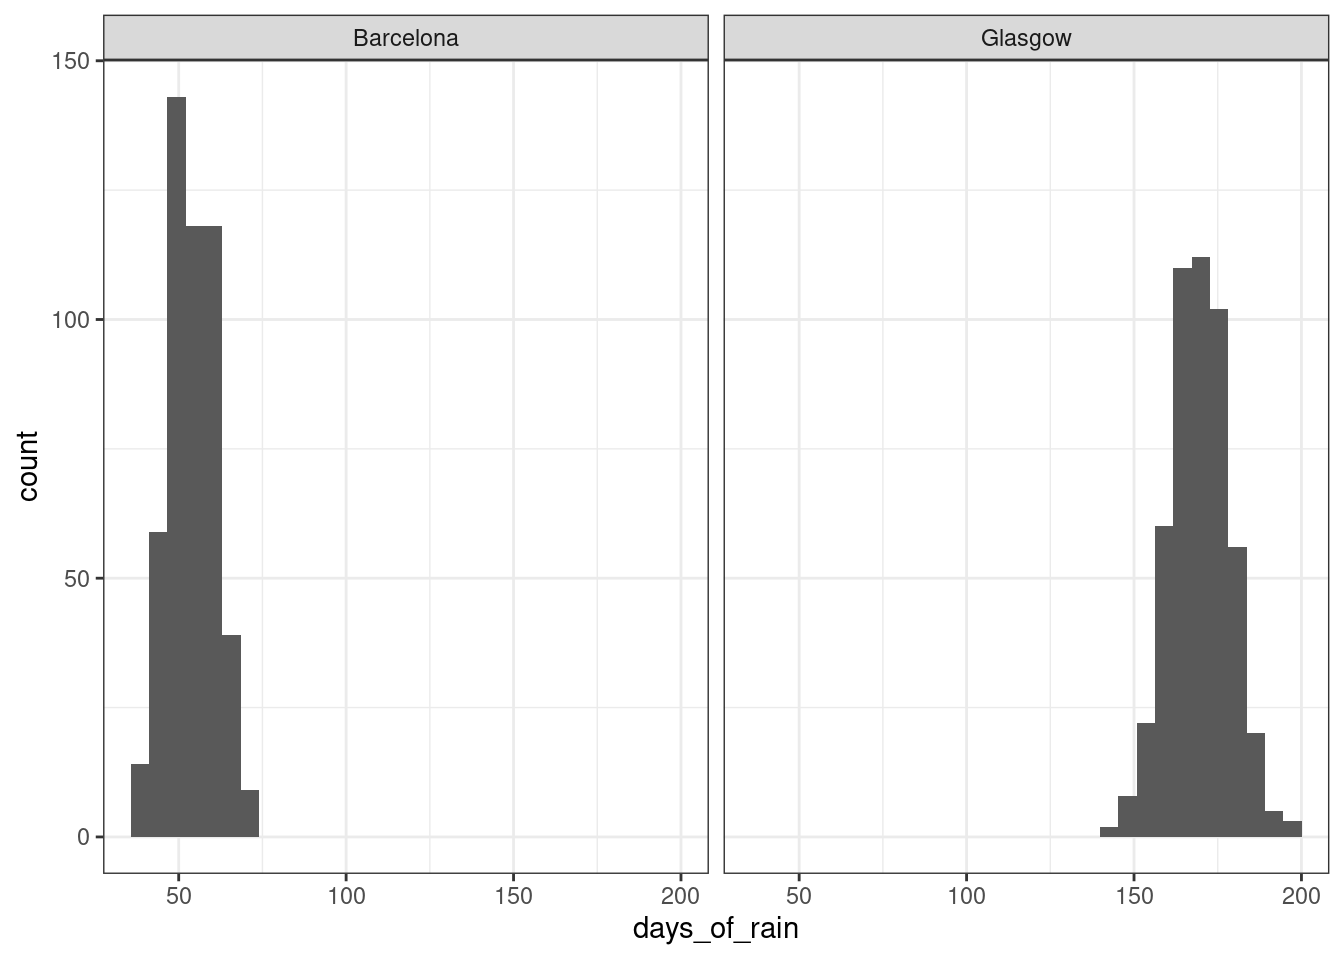
\includegraphics[width=1\linewidth]{08-generalized-linear-models_files/figure-latex/rbinom-1} 

}

\caption{**Distribution of number of rainy days for 500 years of simulated rainfall in Barcelona and Glasgow**}\label{fig:rbinom}
\end{figure}

The distribution for Glasgow is slightly fatter than the distribution for Barcelona. We can also see the greater variability in Glasgow if we look at the standard deviations of these variables.

\begin{Shaded}
\begin{Highlighting}[]
\NormalTok{rainy_days }\OperatorTok
\StringTok{  }\KeywordTok{group_by}\NormalTok{(city) }\OperatorTok
\StringTok{  }\KeywordTok{summarise}\NormalTok{(}\DataTypeTok{sd =} \KeywordTok{sd}\NormalTok{(days_of_rain))}
\end{Highlighting}
\end{Shaded}

\begin{verbatim}
## `summarise()` ungrouping output (override with `.groups` argument)
\end{verbatim}

\begin{verbatim}
## # A tibble: 2 x 2
##   city         sd
##   <chr>     <dbl>
## 1 Barcelona  6.68
## 2 Glasgow    9.19
\end{verbatim}

\hypertarget{spurious-interactions-due-to-scaling-effects}{%
\subsubsection{Spurious interactions due to scaling effects}\label{spurious-interactions-due-to-scaling-effects}}

Another reason why treating discrete data as continuous can be problematic is the bounded nature of many discrete scales, which can lead to the detection of spurious interaction effects. For instance, consider the effect of some experimental intervention that increases accuracy. If participants are already highly accurate (e.g., more than 90\%) in condition A than in condition B (say, 50\%) then the size of the possible effect in A is smaller than the size of the possible effect in B, since accuracy cannot exceed 100\%. Thus, it is difficult to know whether any interaction effect reflects something theoretically meaningful, or just an artifact of the bounded nature of the scale.

\hypertarget{generalized-linear-models}{%
\section{Generalized Linear Models}\label{generalized-linear-models}}

The basic idea behind Generalized Linear Models (not to be confused with General Linear Models) is to specify a \textbf{link function} that transforms the response space into a modeling space where we can perform our usual linear regression, and to capture the dependence of the variance on the mean through a \textbf{variance function}. The parameters of the model will be expressed on the scale of the modeling space, but we can always transform it back into our original response space using the \textbf{inverse link function}.

There are a large variety of different kinds of generalized linear models you can fit to different types of data. The ones most commonly used in psychology are \textbf{logistic regression} and \textbf{Poisson regression}, the former being used for binary data (Bernoulli trials) and the latter being used for count data, where the number of trials is not well-defined. We will be focusing on logistic regression.

\hypertarget{logistic-regression}{%
\section{Logistic regression}\label{logistic-regression}}

\hypertarget{terminology}{%
\subsection{Terminology}\label{terminology}}

\begin{tabular}{l|l}
\hline
Term & Definition\\
\hline
**Bernoulli trial** & An event with a binary outcome, with one outcome considered 'success'\\
\hline
**proportion** & The ratio of successes to the total number of Bernoulli trials\\
\hline
**odds** & The ratio of successes to failures\\
\hline
**log odds** & The (natural) log of the odds\\
\hline
\end{tabular}

In logistic regression, we are modeling the relationship between the response and a set of predictors in log odds space.

Logistic regression is used when the individual outcomes are Bernoulli trials---events with binary outcomes. Typically one of the two outcomes is referred to as `success' and is coded as a 1; the other is referred to as `failure' and is coded as 0. Note that the terms `success' and `failure' are completely arbitrary, and should not be taken to imply that the more desireable category should always be coded as 1. For instance, when flipping a coin we could equivalently choose `heads' as success and `tails' as failure or vice-versa.

Often the outcome of a sequence of Bernoulli trials is communicated as a \textbf{proportion}---the ratio of successes to the total number of trials. For instance, if we flip a coin 100 times and get 47 heads, we would have a proportion of 47/100 or .47, which would also be our estimate of the probability of the event. For events coded as 1s and 0s, a shortcut way of getting the proportion is to use the \texttt{mean()} function.

We can also talk about the odds of success, i.e., that the odds of heads versus tails are one to one, or 1:1. The odds of it raining on a given day in Glasgow would be 170:195; the denominator is the number of days it did not rain (365 - 170 = 195). Expressed as a decimal number, the ratio 170/195 is about 0.87, and is known as the \textbf{natural odds}. Natural odds ranges from 0 to \(+\inf\). Given \(Y\) successes on \(N\) trials, we can represent the natural odds as \(\frac{Y}{N - Y}\). Or, given a probability \(p\), we can represent the odds as \(\frac{p}{1-p}\).

The natural log of the odds, or \textbf{logit} is scale on which logistic regression is performed. Recall that the logarithm of some value \(Y\) gives the exponent that would yield \(Y\) for a given base. For instance, the \(log_2\) (log to the base 2) of 16 is 4, because \(2^4 = 16\). In logistic regression, the base that is typically used is \(e\) (also known as Euler's number). To get the log odds from odds of, say, Glasgow rainfall, we would use \texttt{log(170/195)}, which yields -0.1372011; to get natural odds back from log odds, we would use the inverse, \texttt{exp(-.137)}, which returns about 0.872.

\hypertarget{properties-of-log-odds}{%
\subsection{Properties of log odds}\label{properties-of-log-odds}}

log odds = \(\log \left(\frac{p}{1-p}\right)\)

Log odds has some nice properties for linear modeling.

First, it is symmetric around zero, and zero log odds corresponds to maximum uncertainty, i.e., a probability of .5. Positive log odds means that success is more likely than failure (Pr(success) \textgreater{} .5), and negative log odds means that failure is more likely than success (Pr(success) \textless{} .5). A log odds of 2 means that success is more likely than failure by the same amount that -2 means that failure is more likely than success. The scale is unbounded; it goes from \(-\infty\) to \(+\infty\).

\hypertarget{link-and-variance-functions}{%
\subsection{Link and variance functions}\label{link-and-variance-functions}}

The link function for logistic regression is:

\[\eta = \log \left(\frac{p}{1-p}\right)\]

while the inverse link function is:

\[p = \frac{1}{1 + e^{-\eta}}\]

where \(e\) is Euler's number. In R, you could type this latter function as \texttt{1/(1\ +\ exp(-eta))}.

The variance function is the variance for the binomial distribution, namely:

\[np(1 - p)\].

The app below allows you to manipulate the intercept and slope of a line in log odds space and to see the projection of the line back into response space. Note the S-shaped (``sigmoidal'') shape of the function in the response shape.

\begin{verbatim}
## PhantomJS not found. You can install it with webshot::install_phantomjs(). If it is installed, please make sure the phantomjs executable can be found via the PATH variable.
\end{verbatim}

\label{fig:logit-app}\textbf{Logistic regression web app} \url{https://shiny.psy.gla.ac.uk/Dale/logit}

\hypertarget{estimating-logistic-regression-models-in-r}{%
\subsection{Estimating logistic regression models in R}\label{estimating-logistic-regression-models-in-r}}

For single-level data, you use the \texttt{glm()} function. Note that it is much like the \texttt{lm()} function you are already familiar with. The main difference is that you specify a \texttt{family} argument for the link/variance functions. For logistic regression, you use \texttt{family\ =\ binomial(link\ =\ "logit")}. The logit link is default for the binomial family with a logit link, so typing \texttt{family\ =\ binomial} is sufficient.

\texttt{glm(DV\ \textasciitilde{}\ IV1\ +\ IV2\ +\ ...,\ data,\ family\ =\ binomial)}

For multi-level data where there are random effects to be modeled, you use the \texttt{glmer} function from \texttt{lme4}:

\texttt{glmer(DV\ \textasciitilde{}\ IV1\ +\ IV2\ +\ ...\ (1\ \textbar{}\ subject),\ data,\ family\ =\ binomial)}

\hypertarget{modeling-ordinal-data}{%
\chapter{Modeling Ordinal Data}\label{modeling-ordinal-data}}

It is perhaps easiest to think about ordinal data by viewing it as a more general case of logistic regression. In logistic regression, the response variable \(Y\) has two categories (e.g., 0, 1), with the model intercept representing the point in log odds space where 0 and 1 are equiprobable.

\[\eta = \beta_0 + \beta_1 X_i\]

\begin{Shaded}
\begin{Highlighting}[]
\NormalTok{xx <-}\StringTok{ }\KeywordTok{rep}\NormalTok{(}\KeywordTok{seq}\NormalTok{(}\DecValTok{1}\NormalTok{, }\DecValTok{3}\NormalTok{, }\DataTypeTok{by =} \FloatTok{.1}\NormalTok{))}
\NormalTok{x2 <-}\StringTok{ }\NormalTok{xx }\OperatorTok{+}\StringTok{ }\DecValTok{3}
\NormalTok{yy <-}\StringTok{ }\KeywordTok{rep}\NormalTok{(}\KeywordTok{seq}\NormalTok{(}\OperatorTok{-}\DecValTok{3}\NormalTok{, }\DecValTok{3}\NormalTok{, }\DataTypeTok{by =} \FloatTok{.1}\NormalTok{))}

\NormalTok{ras <-}\StringTok{ }\KeywordTok{bind_rows}\NormalTok{(}\KeywordTok{crossing}\NormalTok{(xx, yy) }\OperatorTok
\StringTok{                 }\KeywordTok{mutate}\NormalTok{(}\DataTypeTok{zz =}\NormalTok{ yy, }\DataTypeTok{cat =}\NormalTok{ 1L),}
                 \KeywordTok{crossing}\NormalTok{(xx, yy) }\OperatorTok
\StringTok{                 }\KeywordTok{mutate}\NormalTok{(}\DataTypeTok{zz =}\NormalTok{ yy }\OperatorTok{+}\StringTok{ }\FloatTok{1.5}\NormalTok{, }\DataTypeTok{cat =}\NormalTok{ 2L))}
          
\KeywordTok{ggplot}\NormalTok{(ras, }\KeywordTok{aes}\NormalTok{(xx, yy)) }\OperatorTok{+}
\StringTok{  }\KeywordTok{geom_raster}\NormalTok{(}\KeywordTok{aes}\NormalTok{(}\DataTypeTok{fill =}\NormalTok{ zz), }\DataTypeTok{interpolate =} \OtherTok{TRUE}\NormalTok{) }\OperatorTok{+}
\StringTok{  }\KeywordTok{scale_fill_gradient2}\NormalTok{(}\DataTypeTok{high =} \StringTok{"green"}\NormalTok{, }\DataTypeTok{low =} \StringTok{"red"}\NormalTok{) }\OperatorTok{+}
\StringTok{  }\KeywordTok{facet_wrap}\NormalTok{(}\OperatorTok{~}\NormalTok{cat)}
\end{Highlighting}
\end{Shaded}

\begin{figure}

{\centering 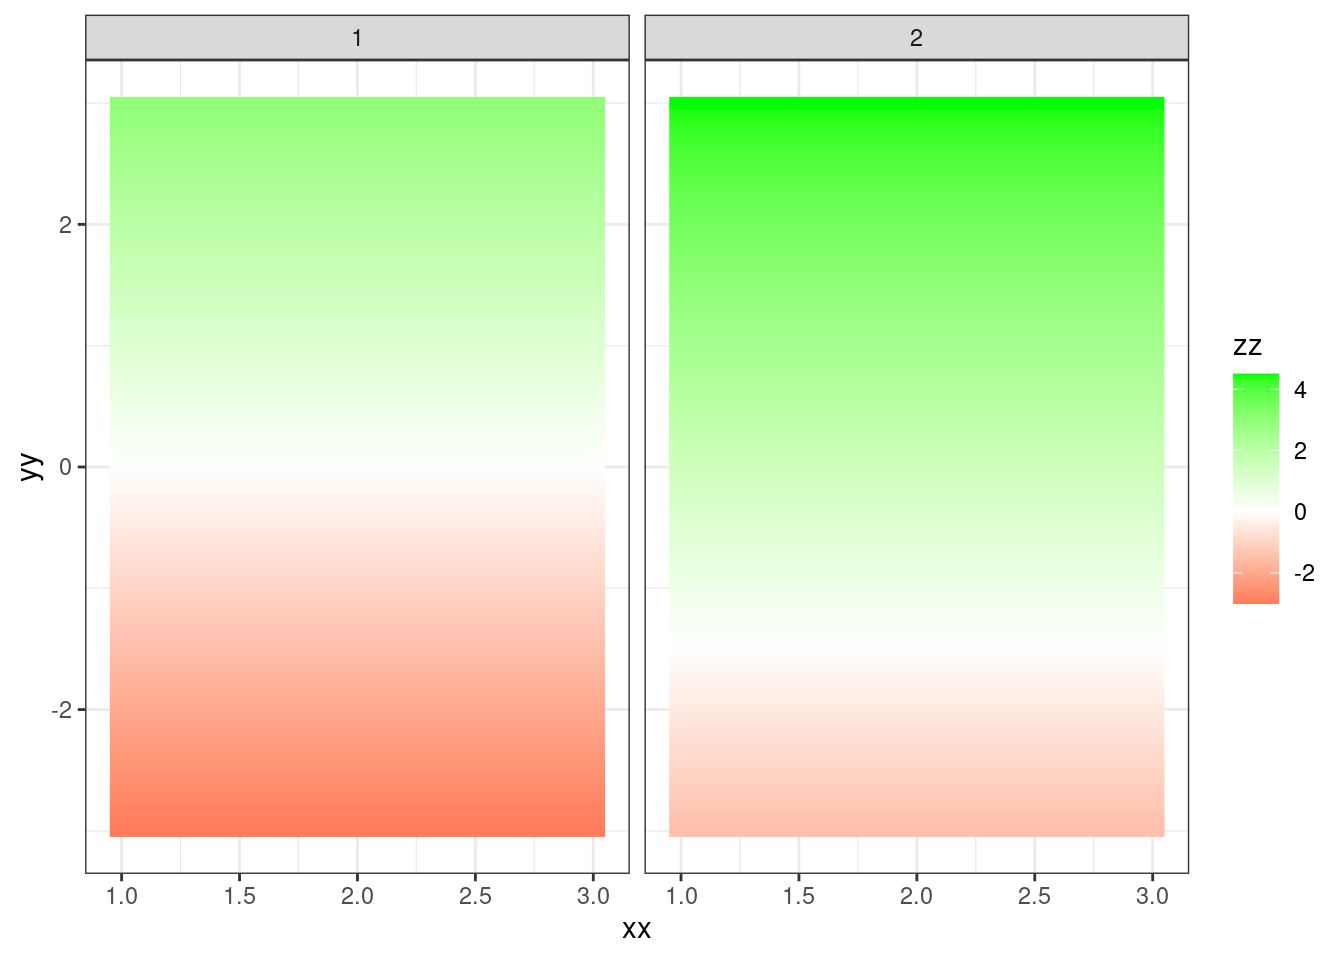
\includegraphics[width=1\linewidth]{09-ordinal_files/figure-latex/start-1} 

}

\caption{TODO}\label{fig:start}
\end{figure}

\hypertarget{appendix-appendix}{%
\appendix}


\hypertarget{symbols}{%
\chapter{Symbols}\label{symbols}}

\hypertarget{general-notes}{%
\section{General notes}\label{general-notes}}

\begin{itemize}
\item
  Greek letters represent population parameter values; roman letters represent sample values.
\item
  A Greek letter with a ``hat'' represents and \emph{estimate} of the population value from the sample; i.e., \(\mu_x\) represents the true population mean of \(X\), while \(\hat{\mu}_x\) represents its estimate from the sample.
\end{itemize}

\hypertarget{table-of-symbols}{%
\section{Table of symbols}\label{table-of-symbols}}

\begin{tabular}{l|l|l}
\hline
symbol & pronunciation & definition\\
\hline
\$\textbackslash{}mu\$ & meeYU & generally, a population mean; sometimes, a model intercept. \$\textbackslash{}mu\_x\$ represents the mean of x\\
\hline
\$\textbackslash{}sigma\$ & sigma & lower case sigma is the standard deviation; \$\textbackslash{}sigma\_x\$ is the standard deviation of \$X\$\\
\hline
\$\textbackslash{}sigma\textasciicircum{}2\$ & sigma squared & variance\\
\hline
\$\textbackslash{}rho\$ & row & population correlation; \$\textbackslash{}rho\_\{xy\}\$ is the correlation in the population between \$X\$ and \$Y\$\\
\hline
\$r\$ & row & sample correlation; r\_\{xy\} is the correlation in the sample between \$X\$ and \$Y\$\\
\hline
\$\textbackslash{}mathbf\{\textbackslash{}Sigma\}\$ & sigma & the capital letter sigma in boldface represents a variance-covariance matrix\\
\hline
\$\textbackslash{}sum\$ & sigma & upper case sigma is an instruction to add; e.g., \$\textbackslash{}sum X\_i\$ is the instruction to sum together all values of X.\\
\hline
\$\textbackslash{}beta\$ & beta & regression coefficient\\
\hline
\$\textbackslash{}sim\$ & is distributed as & e.g., \$e \textbackslash{}sim N\textbackslash{}left(\textbackslash{}mu, \textbackslash{}sigma\textasciicircum{}2\textbackslash{}right)\$ means that \$e\$ is distributed as a Normal distribution with mean \$\textbackslash{}mu\$ and variance \$\$\textbackslash{}sigma\textasciicircum{}2\$\$\\
\hline
\$\textbackslash{}gamma\$ & gamma & fixed effects, correlation coefficients in a mixed-effects regression\\
\hline
\$\textbackslash{}tau\$ & tau & by-subject variance component (random effects parameter) in a mixed-effects regression\\
\hline
\$\textbackslash{}omega\$ & omega & by-stimulus variance component (random effects parameter) in a mixed-effects regression\\
\hline
\$S\_\{0s\}\$ & S sub zero S & by-subject random intercept effect for subject \$s\$\\
\hline
\$S\_\{1s\}\$ & S sub one S & by-subject random slope effect for subject \$s\$\\
\hline
\end{tabular}

\hypertarget{bibliography}{%
\chapter{Bibliography}\label{bibliography}}

\bibliography{book.bib,packages.bib}

\end{document}
